\documentclass[11pt,oneside]{book}
\usepackage{fontspec}
\usepackage[CJKspace]{xeCJK}
\setmainfont{Latin Modern Roman}
\setCJKmainfont[ItalicFont={Noto Serif CJK KR},BoldItalicFont={Noto Serif CJK KR Bold}]{Noto Serif CJK KR}
\setCJKsansfont{Noto Sans CJK KR}
\setCJKmonofont{Noto Sans Mono CJK KR}
\newfontfamily\proseunicodefont{DejaVu Serif}
\usepackage[margin=1in]{geometry}
\usepackage{microtype}
\usepackage{amsmath,amssymb,amsthm,mathtools,bm}
\usepackage{graphicx}
\usepackage{adjustbox}
\usepackage{xcolor}
\usepackage{booktabs}
\usepackage{array}
\usepackage{longtable}
\usepackage{enumitem}
\usepackage{float}
\usepackage{caption}
\usepackage{hyperref}
\usepackage{fancyhdr}
\usepackage{tikz}
\usetikzlibrary{arrows.meta,positioning,calc,decorations.pathmorphing}

\hypersetup{
  colorlinks=true,
  linkcolor=blue!50!black,
  urlcolor=blue!50!black,
  citecolor=blue!50!black
}

\setlength{\parskip}{0.5em}
\setlength{\parindent}{0pt}
\setlist[itemize]{topsep=0.25em,itemsep=0.2em}
\setlist[enumerate]{topsep=0.25em,itemsep=0.2em}
\setlength{\headheight}{40pt}
\numberwithin{equation}{chapter}

\newtheorem{theorem}{정리}[chapter]
\newtheorem{proposition}[theorem]{명제}
\newtheorem{lemma}[theorem]{보조정리}
\newtheorem{corollary}[theorem]{따름정리}
\theoremstyle{definition}
\newtheorem{definition}[theorem]{정의}
\newtheorem{example}[theorem]{예}
\theoremstyle{remark}
\newtheorem{remark}[theorem]{비고}

\providecommand{\ket}[1]{\left\lvert#1\right\rangle}
\providecommand{\bra}[1]{\left\langle#1\right\rvert}
\providecommand{\braket}[2]{\left\langle#1\,\middle|\,#2\right\rangle}
\providecommand{\expect}[1]{\left\langle#1\right\rangle}
\newcommand{\lectureoverview}[1]{\paragraph{개요.} #1}

\makeatletter
\newcommand{\course@headerfont}{\normalfont\small\itshape}
\newcommand{\course@pagefont}{\normalfont\small}
\newcommand{\course@headerraise}{14pt}
\newlength{\course@headerboxheight}
\setlength{\course@headerboxheight}{\dimexpr\headheight-\course@headerraise-9pt\relax}
\newcommand{\course@leftheadbox}[1]{%
  \raisebox{\course@headerraise}{%
    \parbox[t][\course@headerboxheight][t]{0.82\textwidth}{%
      \raggedright\course@headerfont\strut\MakeUppercase{#1}\strut%
    }%
  }%
}
\newcommand{\course@rightheadbox}[1]{%
  \raisebox{\course@headerraise}{%
    \parbox[t][\course@headerboxheight][t]{0.82\textwidth}{%
      \raggedleft\course@headerfont\strut\MakeUppercase{#1}\strut%
    }%
  }%
}
\renewcommand{\chaptermark}[1]{\markboth{\MakeUppercase{\chaptername\ \thechapter.\ #1}}{}}
\renewcommand{\sectionmark}[1]{\markright{\MakeUppercase{\thesection\hspace{0.4em}#1}}}
\fancyhf{}
\fancyhead[L]{\course@leftheadbox{\leftmark}}
\fancyhead[R]{\course@pagefont\thepage}
\renewcommand{\headrulewidth}{0.5pt}
\pagestyle{fancy}
\fancypagestyle{plain}{%
  \fancyhf{}
  \fancyhead[L]{\course@leftheadbox{\leftmark}}
  \fancyhead[R]{\course@pagefont\thepage}
  \renewcommand{\headrulewidth}{0.5pt}
}
\makeatother

% Video2Book editorial provenance macros
\newenvironment{classroomqa}{%
  \par\medskip\noindent\begin{minipage}{\linewidth}\small\hrule\medskip
}{%
  \medskip\hrule\end{minipage}\par\medskip
}
\newcommand{\audiencequestion}[1]{\noindent\textbf{청중 질문.} #1\par\smallskip}
\newcommand{\lecturerresponse}[1]{\noindent\textbf{답변.} #1\par}
\newcommand{\lecturetimestamp}[1]{\footnote{강의 시각: #1.}}
\newcommand{\lectureframe}[1]{\par\smallskip{\centering\footnotesize\itshape 강의 화면: #1.\par}}
\newcommand{\editorialnote}[1]{\footnote{편집자 설명: #1}}

\renewcommand{\contentsname}{목차}
\renewcommand{\chaptername}{장}
\renewcommand{\figurename}{그림}
\renewcommand{\tablename}{표}
\renewcommand{\proofname}{증명}
\renewcommand{\bibname}{참고문헌}
\emergencystretch=2em
\pdfstringdefDisableCommands{\def\proseunicodefont{}}

\geometry{paperwidth=177.6mm,paperheight=252mm,left=16mm,right=16mm,
 top=18mm,bottom=18mm,includeheadfoot,headheight=28pt,headsep=7mm,footskip=9mm}
\usepackage{scrextend}
\changefontsizes[17pt]{12pt}
\raggedbottom
\renewenvironment{classroomqa}{\par\medskip\begingroup}{\par\endgroup\medskip}
\fancyhf{}
\setlength{\headwidth}{\textwidth}
\fancyhead[L]{\parbox{\textwidth}{\raggedright\fontsize{9}{11}\selectfont\nouppercase{\leftmark}}}
\fancyfoot[C]{\small\thepage}
\renewcommand{\headrulewidth}{0.3pt}
\fancypagestyle{plain}{\fancyhf{}\fancyfoot[C]{\small\thepage}\renewcommand{\headrulewidth}{0pt}}

\graphicspath{{../../../generated_course_notes/supplementary/particle_physics_2_standard_model/2010_winter/figures/}{../../../generated_course_notes/supplementary/particle_physics_2_standard_model/2010_winter/assets/}}
\begin{document}
\frontmatter
\hypersetup{pageanchor=false}
\begin{titlepage}
\hyphenpenalty=10000\exhyphenpenalty=10000
\thispagestyle{empty}
\begin{tikzpicture}[remember picture,overlay]
  \node[anchor=center,inner sep=0] at (current page.center) {%
    \includegraphics[height=\paperheight,keepaspectratio]{../../../generated_course_notes/supplementary/particle_physics_2_standard_model/2010_winter/assets/cover-art.png}%
  };
  \node[
    anchor=north west,
    align=left,
    text width=0.78\paperwidth,
    fill=white,
    fill opacity=0.9,
    rounded corners=8pt,
    inner xsep=10pt,
    inner ysep=8pt
  ] at ([xshift=0.08\paperwidth,yshift=-0.06\paperheight]current page.north west) {%
    {\fontsize{30}{33}\selectfont\bfseries\color{black!88} 입자물리학 2: 표준모형\\[0.85em]}
    {\large\color{black!72} 한국어판 / 2010년 겨울}
  };
  \node[
    anchor=south west,
    align=left,
    text width=0.68\paperwidth,
    fill=white,
    fill opacity=0.82,
    text opacity=1,
    rounded corners=6pt,
    inner sep=12pt
  ] at ([xshift=0.08\paperwidth,yshift=0.08\paperheight]current page.south west) {%
    {\normalsize\color{black!78} 원 강의: Leonard Susskind\\[0.35em]}
    {\small\color{black!72} 보조 강의 노트: \href{https://lazying.art}{LazyingArt LLC} / \href{https://github.com/lachlanchen/Video2Book}{Video2Book}}
  };
\end{tikzpicture}
\mbox{}
\end{titlepage}
\hypersetup{pageanchor=true}

\clearpage
\chapter{이 노트에 관하여}
이 보조 강의 노트는 Leonard Susskind의 강의를 바탕으로 독립적으로 편집한 자료입니다. 기계가 생성한 녹취록과 자막, 일부 칠판 화면을 토대로 내용을 재구성한 뒤, 이용 가능한 원자료와 대조해 확인했습니다. 이 자료는 Susskind 교수의 원고가 아니며, 교수의 검토나 승인을 받지 않았습니다.

이 판본은 \href{https://lazying.art}{LazyingArt LLC}에서 오픈 소스 \href{https://github.com/lachlanchen/Video2Book}{Video2Book} 워크플로를 사용해 제작했습니다. 기계가 생성한 녹취록은 별도로 제공되며, 인식 오류가 있을 수 있습니다. 편집상 명확히 한 부분과 상당한 재구성이 이루어진 부분은 각주에 표시했습니다.
\clearpage
\tableofcontents
\mainmatter
\chapter{힘, 쿼크, 그리고 최초의 강입자 다중항}

\section{입자, 장, 그리고 빠진 세 번째 요소}

파동은 장의 배열이므로, 이 논의에서는 두 설명이 밀접하게 관련되어 있다. 양자역학에 따르면 그런 파동의 에너지는 불연속적인 불가분 단위로 주어진다. 이 단위가 양자이며, 장의 양자가 바로 입자라고 부르는 것이다. 이 관계를 바탕으로 우리는 이미 파동방정식, 작용 원리, 그리고 입자가 지니는 에너지, 운동량, 스핀, 보손--페르미온 구분 같은 전반적인 성질을 논의했다. 페르미온은 같은 상태를 점유하는 것을 꺼리는 반면, 보손은 한 상태에 모여 응축할 수 있다.

양자 라그랑지안에는 상호작용도 기록된다. 장의 곱은 입자가 들어오고 나가는 꼭짓점을 나타낸다. 예를 들어 장의 네 제곱을 포함하는 항은 네 다리 상호작용 꼭짓점을 나타낸다. 이처럼 작용 원리는 가능한 입자 과정의 목록을 간결하게 정리한다.

다음 과제는 입자들의 이름을 붙이고------각 입자에 고유한 성격, 즉 성질과 상호작용, 일상적인 물리에서의 역할을 부여하는 것이다. 하지만 그 목록을 만들기 전에 개념적 삼각형의 한 변이 아직 빠져 있다.
\begin{itemize}
\item 입자,
\item 그 입자들이 양자인 장,
\item 바로 그 양자들이 관여하는 교환 과정과 관련된 힘.
\end{itemize}

\emph{기본}이라는 말은 잠정적으로만 써야 한다. 복합 입자와 구별되는 기본 입자를 정의하려 하면, 그럴듯한 정의는 결국 모호한 사례와 마주치게 된다. 이 문제는 뒤에서 다시 다루겠다. 지금은 기본 장이 존재한다고 가정하고, 그 양자를 기본 입자라고 부르자. 전기장이 전기력을 일으키고 중력장이 중력을 일으킨다면, 전자장도 힘에 관여해야 한다. 힘을 장으로 설명하는 동시에 입자로도 설명할 수 있어야 이 삼각형이 닫힌다.

그러므로 힘의 논리를 두 번 유도하겠다. 먼저 고전 장 에너지를 이용한 다음, 장을 양자로 분해했을 때 같은 상호작용이 어떻게 나타나는지 살펴본다. 이 두 설명을 잇는 가교가 확실해진 뒤에야 입자 목록을 시작하겠다.

\section{고전 전기역학에서 장 에너지로부터 힘을 구하기}

공간에 두 전하를 놓아 보자. 두 전하 사이의 힘을 구하는 한 방법은 역제곱 법칙을 인용하는 것이다. 더 많은 것을 보여 주는 방법은 전하가 공간에 어떤 영향을 주는지 묻는 것이다. 전하는 전기장을 만들고, 그 장은 에너지를 저장한다.

각 전하와 그 전하가 만드는 장의 공간적 형태를 분리해 두는 것이 편리하다.
\begin{equation}
\mathbf E_i=q_i\widehat{\mathbf E}_i,
\end{equation}
모자 표기를 유지하는지는 결과에 영향을 주지 않는다. 두 전하가 모두 있을 때 선형성에 따라
\begin{equation}
\mathbf{E}=\mathbf{E}_1+\mathbf{E}_2.
\end{equation}
단위계 선택에 따른 차이를 제외하면 정전기장의 에너지는 다음 형태를 갖는다.
\begin{equation}
U_{\text{field}}\propto\int d^3x\,\mathbf{E}^2.
\end{equation}
두 장의 합을 대입하면
\begin{align}
U_{\text{field}}
&\propto\int d^3x\,(\mathbf{E}_1+\mathbf{E}_2)^2 \\
&\propto\int d^3x\,\bigl(\mathbf{E}_1^2+\mathbf{E}_2^2
  +2\mathbf{E}_1\!\cdot\!\mathbf{E}_2\bigr).
\end{align}

앞의 두 항은 자기 에너지다. 어느 한 전하를 옮기면 그 전하의 장도 함께 이동하므로, 해당 적분값은 변하지 않는다. 이 에너지는 \(E=mc^2\)를 통해 고립된 대전 입자의 측정 질량에 기여한다. 이 자기 에너지가 측정 질량에 어떻게 반영되는지는 나중에 다룰 재규격화의 주제다. 위치에 무관한 이 에너지는 어느 것도 두 입자 사이의 힘에 기여하지 않는다.

교차항은 다르다. 이 항은 어느 한 입자에만 속하지 않으며 두 장이 모두 있을 때에만 존재한다. 두 전하를 아주 멀리 떨어뜨리면 유의미한 장 영역은 거의 겹치지 않는다. 전하가 가까워지면 겹치는 정도가 달라진다. 따라서 배열에 따라 달라지는 상호작용 에너지는 다음에 비례한다.
\begin{equation}
U_{\text{int}}(r)\propto q_1q_2\int d^3x\,
\widehat{\mathbf E}_1\!\cdot\!\widehat{\mathbf E}_2.
\end{equation}
두 점전하 사이의 거리가 \(r\)일 때 적분을 계산하면 익숙한 의존성이 나온다.
\begin{equation}
U_{\text{int}}(r)\propto\frac{q_1q_2}{r}.
\end{equation}
방사 방향 힘은 이 에너지의 음의 기울기다.
\begin{equation}
\mathbf F_{12}=-\boldsymbol\nabla_{\mathbf r}U_{\text{int}},
\qquad
|\mathbf F_{12}|\propto\frac{|q_1q_2|}{r^2}.
\end{equation}
\editorialnote{강의에서 말로 설명한 논증은 퍼텐셜을 따로 거치지 않고 교차항을 역제곱 쿨롱 힘과 연결한다. 여기서는 그 기울기가 명시된 \(1/r^2\) 힘을 주도록 표준적인 중간 단계인 \(U_{\mathrm{int}}\propto1/r\)를 적어 둔다.}

힘의 법칙은 이제 상대적 위치에 따라 달라지는 장 에너지 부분의 미분으로 표현된다. 두 물체가 멀리 떨어져 있으면 사실상 서로 독립적이다. 두 물체를 가까이 가져오면 그 사이의 장이 재배열되고, 그 결과 에너지가 변한다. 이것이 상호작용이다.

하지만 장을 양자로 분해할 수 있다면, 이것으로 이야기가 끝날 수는 없다. 같은 힘을 입자의 언어로도 설명할 수 있어야 한다.

\section{분자 교환: 양성자 두 개와 전자 한 개}

전기역학으로 돌아가기 전에 교환을 더 쉽게 그려 볼 수 있는 계, 즉 양성자 두 개와 전자 한 개로 이루어진 계를 살펴보자. 교환은 분자력의 여러 기원 가운데 하나일 뿐이지만, 이 예에서는 교환과 에너지, 힘의 관계를 분명히 볼 수 있다. 이 예는 양자전기역학을 대신하려는 것이 아니다.

양성자 하나만 있고 다른 양성자가 무한히 멀리 떨어져 있다면, 전자는 첫 번째 양성자에 중심을 둔 수소형 바닥 상태를 차지할 수 있다. 그 파동함수는 해당 힘의 중심 부근에 국소화되어 있다.

\begin{figure}[h]
\centering
\includegraphics[width=0.72\textwidth]{lecture_01_figure_02.png}

\medskip

\begin{tikzpicture}[scale=0.95]
\draw (-0.2,0) -- (6.4,0);
\fill (1.3,0) circle (2pt);
\draw[smooth] plot coordinates {(0.1,0.15) (0.8,1.15) (1.5,1.75) (2.2,1.1) (3.0,0.35) (3.8,0.12)};
\node at (1.3,-0.35) {$p$};
\node at (2.7,1.55) {$\psi_1(x)$};
\end{tikzpicture}
\caption{한 양성자 부근에 국소화된 수소형 바닥 상태 파동함수.}
\lectureframe{00:14:32}
\end{figure}
\editorialnote{다시 그린 그림의 \(\psi_1(x)\) 표기는 00:14:30에서 설명한 국소화된 형태를 가리킨다. 읽을 수 있는 판서의 표기를 옮긴 것은 아니다.--00:14:32}

이제 두 번째 양성자를 유한하지만 큰 거리에 놓자. 대칭성에 따라 같은 한 중심 에너지를 갖는 두 번째 국소화 상태가 생기며, 이번에는 오른쪽 양성자를 중심으로 한다.

\begin{figure}[h]
\centering
\includegraphics[width=0.78\textwidth]{lecture_01_figure_03.png}

\medskip

\begin{tikzpicture}[scale=0.92]
\draw (-0.2,0) -- (9.0,0);
\fill (1.4,0) circle (2pt);
\fill (7.4,0) circle (2pt);
\draw[smooth] plot coordinates {(0.2,0.2) (0.9,1.05) (1.6,1.55) (2.4,1.0) (3.3,0.35) (4.2,0.12)};
\draw[smooth] plot coordinates {(4.8,0.12) (5.7,0.35) (6.6,1.0) (7.3,1.55) (8.1,1.05) (8.8,0.2)};
\node at (1.4,-0.35) {$p$};
\node at (7.4,-0.35) {$p$};
\node at (2.6,1.45) {$\psi_1(x)$};
\node at (6.2,1.45) {$\psi_2(x)$};
\end{tikzpicture}
\caption{터널링을 허용한 뒤 평형 중첩 상태를 만드는 데 사용되는 두 국소화 파동함수.}
\lectureframe{00:17:54}
\end{figure}
\editorialnote{표기 \(\psi_1(x)\)와 \(\psi_2(x)\)는 00:17:41에서 논의한 두 형태를 가리킨다. 기호는 읽기 쉽도록 덧붙인 개략적인 표기다.--00:17:56}

거리가 무한대일 때 두 상태는 축퇴되어 있다. 전자를 왼쪽이나 오른쪽에 국소화해도 에너지는 같다. 거리가 유한하면 새로운 과정이 가능해진다. 전자는 고전적으로 금지된 영역을 지나 한 중심에서 다른 중심으로 터널링할 수 있다. 장벽을 통과하는 궤적을 관찰하려 하면 상태를 교란하게 된다. ``도약''은 고전적 경로를 촬영한 영상이 아니라 양자적 시간 전개의 설명이다.

평형 상태에서 전자는 두 양성자 가운데 어느 쪽 부근에서 발견될 확률도 같다. 따라서 정규화 계수는 \(1/\sqrt2\)이며, 더 낮은 평형 상태는 근사적으로 다음과 같다.
\begin{equation}
\psi_+(x)\approx \frac{\psi_1(x)+\psi_2(x)}{\sqrt2}.
\end{equation}

근사 기호가 중요하다. 실제 두 중심 파동함수는 변형되지 않은 두 수소형 궤도함수의 합과 정확히 같지 않으며, 겹침 영역에서 모양이 조정된다. 여기서 필요한 요점은 대칭 평형 상태의 에너지가 고립된 한 중심의 에너지보다 낮다는 것이다. 해밀토니안으로 표현하면 왼쪽과 오른쪽 배열은 비대각 행렬 원소로 결합되어 있다. 전자가 두 상태의 결맞은 중첩을 차지하도록 허용하면 에너지가 낮아진다.

\section{낮아진 에너지에서 유효 힘으로}

양성자 사이의 거리가 클 때 전자로 인해 생기는 기여분 \(E_e(r)\)는 분리된 원자의 값에 가까워진다. 거리가 줄면 터널링과 중첩으로 이 값이 낮아진다. 두 양성자--와 전자 하나로 이루어진 계의 전체 퍼텐셜에는 양성자 사이의 직접적인 반발도 포함되어야 한다.
\begin{equation}
V_{\mathrm{tot}}(r)=V_{pp}(r)+E_e(r).
\end{equation}

이로써 분자 예시는 장 에너지 논증과 다시 연결된다. 파동함수 그림과 \(E_e(r)\)의 정성적 곡선은 같은 계산을 두 가지 방식으로 보여 준다. 평형은 두 기여분의 합인 \(V_{\mathrm{tot}}(r)\)로 결정된다.

\begin{figure}[h]
\centering
\includegraphics[width=0.78\textwidth]{lecture_01_figure_04.png}

\medskip

\begin{tikzpicture}[scale=0.9]
\draw (-0.2,3.0) -- (9.0,3.0);
\fill (1.3,3.0) circle (2pt);
\fill (7.3,3.0) circle (2pt);
\draw[smooth] plot coordinates {(0.1,3.15) (0.9,4.0) (1.7,4.45) (2.6,3.9) (3.7,3.25) (4.6,3.08)};
\draw[smooth] plot coordinates {(4.8,3.08) (5.9,3.25) (7.0,3.9) (7.8,4.45) (8.6,4.0) (9.0,3.15)};
\node at (1.3,2.65) {$p$};
\node at (7.3,2.65) {$p$};

\draw[->] (0.2,0.1) -- (0.2,2.0);
\draw[->] (0.2,0.1) -- (8.8,0.1);
\draw[dashed] (0.5,1.48) -- (8.5,1.48);
\draw[smooth] plot coordinates {(0.5,0.38) (1.6,0.56) (2.8,0.82) (4.1,1.08) (5.5,1.27) (6.9,1.39) (8.4,1.44)};
\node at (5.8,1.02) {$E_e(r)$};
\node at (8.8,-0.18) {$r$};
\end{tikzpicture}
\caption{위쪽은 파동함수의 겹침, 아래쪽은 전자로 인해 생기는 에너지를 나타낸다. \(r\)가 증가하면 분리된 원자의 점근값에 가까워지며, 양성자 전체 퍼텐셜에는 양성자 사이의 쿨롱 반발도 포함해야 한다.}
\lectureframe{00:20:28}
\end{figure}
\editorialnote{표기 \(E_e(r)\)와 \(r\)는 00:19:12에서 논의한 에너지 곡선과 거리를 가리킨다. 남아 있는 판서 화면으로는 축 표기를 읽을 수 없다.--00:20:38}

두 힘은 각각 에너지의 기울기로부터 나온다.
\begin{equation}
F_{e}(r)=-\frac{dE_e}{dr},
\qquad
F_{\mathrm{tot}}(r)=-\frac{dV_{\mathrm{tot}}}{dr}.
\end{equation}
따라서 계는 전체 에너지가 낮아지는 방향으로 힘을 받는다. 양성자들이 가까워질수록 \(E_e(r)\)가 감소하는 범위에서는 교환이 인력 성분을 제공한다. 결합된 거리가 존재하는지는 이 인력 성분과 \(V_{pp}(r)\) 사이의 경쟁에 달려 있다. 이것이 공유 결합의 기본 메커니즘이다. 전자가 공유 상태에 있는 까닭은 그 상태의 에너지가 더 낮기 때문이다.

고전적 계산에서는 전기장이 겹치면서 에너지가 달라진다. 여기서는 두 힘의 중심이 더 낮은 양자 상태를 가능하게 한다. 두 메커니즘 모두 평형 에너지가 배열에 따라 달라지기 때문에 힘을 만들어 낸다.

교환을 나타내는 세계선 그림으로 이 설명을 요약할 수 있다. 이를 관측된 궤적으로 읽어서는 안 된다. 전자가 어느 쪽 양성자와 결부될 수 있는지를 나타내는 진폭을 표현한 그림이다.

\begin{figure}[h]
\centering
\begin{tikzpicture}[scale=1.0]
\draw (0,0) -- (0,4.4);
\draw (4.8,0) -- (4.8,4.4);
\draw (0,0.9) .. controls (1.6,1.7) and (3.2,1.7) .. (4.8,2.5);
\draw (4.8,2.9) .. controls (3.2,2.1) and (1.6,2.1) .. (0,3.9);
\node at (0,-0.35) {$p$};
\node at (4.8,-0.35) {$p$};
\node at (2.35,1.55) {$e^-$};
\node at (2.35,2.55) {$e^-$};
\end{tikzpicture}
\caption{두 양성자 세계선 사이의 전자 교환. 관찰된 경로가 아니라 양자 진폭을 나타내는 개략도다.}
\end{figure}

\begin{classroomqa}
\audiencequestion{전자가 양성자 전하를 가리거나 줄여서 인력을 간단히 설명할 수 있나요?\lecturetimestamp{00:23:26}}
\lecturerresponse{아니요. 이 효과를 전하가 줄어드는 그림으로 설명하는 것은 적절하지 않습니다. 핵심은 두 국소화 파동함수를 더해 얻는 상태의 에너지가 각 국소화 상태의 에너지보다 조금 낮다는 점입니다.}
\end{classroomqa}

\begin{classroomqa}
\audiencequestion{파인먼이 ``빛은 빛을 좋아한다''고 한 말이 이런 뜻인가요?\lecturetimestamp{00:23:51}}
\lecturerresponse{아니요. 그 표현은 보손 통계와 관련이 있을 가능성이 큽니다. 광자는 같은 상태를 선호하는 반면 전자는 배타 원리를 따릅니다. 여기서 다루는 분자 효과는 두 중심 사이의 터널링입니다.}
\end{classroomqa}

두 양성자는 여전히 정전기적으로 서로 밀어낸다. 교환의 작용 범위는 쿨롱 상호작용보다 짧으므로, 어느 한 기여분만이 아니라 전체 퍼텐셜을 고려해야 한다. 적절한 거리에서는 분자 이온 \(\mathrm H_2^+\)이 그래도 결합 상태를 이룬다. 중성인 두 전자 계에서는 장거리 전하 반발이 없으므로 공유 결합이 더 익숙한 현상이다.

\begin{classroomqa}
\audiencequestion{양성자 사이에 전자를 두면 주로 정전기적 반발이 줄어드나요?\lecturetimestamp{00:24:33}}
\lecturerresponse{반발이 조금 줄기는 하지만, 그것이 주된 효과는 아닙니다. 전자 교환은 쿨롱 반발보다 작용 범위가 짧은 힘입니다. 장거리 정전기력이 원자 사이에 작용하지 않으면서도 터널링이 인력을 만드는 중성 두 전자 계에서 그 효과가 가장 뚜렷하게 나타납니다.}
\end{classroomqa}

\begin{classroomqa}
\audiencequestion{전자 하나만 가진 양전하 분자 이온 \(\mathrm H_2^+\)은 실제로 결합 상태인가요?\lecturetimestamp{00:26:06}}
\lecturerresponse{네. 충분히 가까운 거리에서는 교환 인력이 양성자--양성자 사이의 쿨롱 반발을 이길 만큼 강해집니다.}
\end{classroomqa}

\begin{classroomqa}
\audiencequestion{두 중심 배열이 세 번째 힘을 만들어 내나요?\lecturetimestamp{00:26:24}}
\lecturerresponse{새로운 기본 힘이 도입되는 것은 아닙니다. 두 양성자의 결합 퍼텐셜 안에서 Schr\"odinger 방정식을 풀면 한 중심 문제와 다른 평형 에너지가 나온다. 달라진 에너지를 미분한 값이 유효 힘이다.}
\end{classroomqa}

\begin{classroomqa}
\audiencequestion{에너지가 낮아지는 것이 양자 얽힘의 한 예인가요?\lecturetimestamp{00:27:06}}
\lecturerresponse{통상적인 두 입자 의미의 얽힘은 아닙니다. 전자 하나만 있으면 됩니다. 여기서 중요한 수학적 특징은 왼쪽 상태와 오른쪽 상태를 결합하는 비대각 해밀토니안 행렬 원소입니다.}
\end{classroomqa}

\begin{classroomqa}
\audiencequestion{온도가 높아지면 교환은 어떻게 되나요?\lecturetimestamp{00:27:37}}
\lecturerresponse{극한적인 고온에서는 전자가 이온화되어 분자와 더는 결부되지 않습니다. 더 낮은 들뜸 에너지에서는 전자가 더 큰 궤도에 있을 수 있으며, 이로 인해 겹침 정도와 힘이 달라집니다. 이는 상태에 따라 달라지는 보정이지, 새로운 일반적 메커니즘은 아닙니다.}
\end{classroomqa}

\section{광자 교환과 표의 첫 항목들}

쿨롱 힘도 같은 교환의 언어로 설명할 수 있을까? 대전 입자는 전자기장과 상호작용하고, 그 장의 양자는 광자다. 고전적으로는 전하 주변의 전기장을 구한다. 양자장론에서는 그 상호작용을 광자의 방출과 흡수로 분해해 기술한다.

실제 대전 입자는 단순히 맨전하만으로 이루어지지 않는다. 그 상태는 맨전자 성분, 광자 하나를 동반한 전자, 광자 둘을 동반한 전자 등을 포함하는 양자 중첩이다. 의도적으로 개략적인 표기법으로 쓰면 다음과 같다.
\begin{equation}
\begin{aligned}
\ket{e_{\mathrm{phys}}}
={}&a_0\ket e
+a_1\ket{e+\text{one photon}}
\\
&+a_2\ket{e+\text{two photons}}+\cdots .
\end{aligned}
\end{equation}
이 표기는 광자 수 성분의 계층만 나타낼 뿐, 광자 운동량을 지정하거나 상호작용하는 대전 상태를 완전히 구성하려는 것은 아니다.
주변 광자는 자유 복사로 빠져나가는 대신 방출되었다가 다시 흡수된다. 그 효과는 측정할 수 있지만 자유롭게 전파하는 광자와 같은 방식으로 검출되지는 않는다. 가까이에 두 번째 전하를 놓으면 한 전하가 방출한 광자를 다른 전하가 흡수할 수 있다. 그러면 두 드레싱된 상태의 에너지는 두 고립된 상태 에너지를 단순히 더한 값과 달라진다.

강의실에서 든 비유는 각자 공을 다루는 저글링하는 사람 둘이다. 두 사람이 멀리 떨어져 있으면 각자 독립적으로 저글링한다. 서로 가까이 오면 한 사람이 다른 사람이 던진 공을 받을 수 있다. 파인먼 도표 언어로 말하면 그 공통 대상은 교환된 광자다. 이 비유는 미시적인 궤적을 뜻하지 않지만, 가까이 있을 때 새로운 과정이 가능해지는 이유를 잘 보여 준다.

이제 쿨롱 법칙을 외우는 데 그치지 않는 두 가지 설명을 얻었다. 고전 장 이론에서는 장들을 더한 뒤 그 결과를 제곱한다. 양자장론에서는 양자가 교환되는 진폭들을 합산한다. 이런 의미에서 입자, 장, 힘은 일대일대일 대응을 이룬다. 전자는 분자 교환을 매개하고, 광자는 전자기 교환을 매개한다. 적절한 상황에서는 교환될 수 있는 입자라면 어느 것이든 고유한 유효 힘 성분에 기여할 수 있다. 따라서 자연에는 네 가지 기본 상호작용이 있다는 익숙한 진술은 더 큰 수준에서 분류한 것이다. 교환의 언어로 보면 교환 가능한 각 종이 그 자체의 유효 힘 성분을 만들어 낼 수 있다.

이제 입자의 이름을 붙이고, 성질을 나열하며, 어떤 과정에 참여할 수 있는지 설명할 차례다. 표준모형 전체를 한 번에 쓰면 긴 암기 시험이 될 뿐이므로, 서로 단순한 관계를 이루는 작은 입자군으로 나누어 각 군이 어떤 일을 할 수 있는지 알아보겠다.

전체 목록은 다소 복잡하다. 왜 바로 이 입자들이 존재하고 상상할 수 있는 다른 입자들은 존재하지 않는지 우리는 이해하지 못하기 때문이다. 수학적 일관성은 몇 가지 관계를 제약한다. 어떤 패턴의 구성원들이 여럿 존재하면, 그 패턴을 완성하기 위해 다른 구성원이 요구될 수도 있다. 이런 관계 덕분에 독립적으로 알아야 할 사실의 수는 줄지만, 그 감소 폭은 크지 않다. 많은 입자 종류와 많은 매개변수가 여전히 설명되지 않았다. 뒤이은 실험이 무엇을 발견하려 하는지 이해하려면 이 미완의 구조를 파악해야 한다.

\begin{figure}[h]
\centering
\includegraphics[width=0.7\textwidth]{lecture_01_figure_05.png}
\caption{입자 표의 첫 항목은 \(\gamma\)로 광자를, 벡터 퍼텐셜 \(A\)로 그 장을 나타낸다.}
\lectureframe{00:39:11}
\end{figure}

첫 장--양자 대응 관계는 다음과 같다.
\begin{equation}
\gamma \leftrightarrow A.
\end{equation}
여기서 \(A\)는 전자기 벡터 퍼텐셜이다. 광자는 전기전하, 바리온 수, 정지 질량이 모두 0인 스핀 1 보손이다. 전자장은 관례적으로 \(\psi_e\)로 표기한다. 전자장의 생성 부분과 소멸 부분은 전자 및 양전자 상태에 작용한다.

우리 표에는 이름, 입자 기호, 장, 보손 또는 페르미온의 종류, 전기전하 \(Q\), 바리온 수 \(B\), 질량을 기록한다.

\begin{table}[h]
\centering
\resizebox{\linewidth}{!}{%
\begin{tabular}{lllllll}
이름 & 기호 & 장 & 종류 & \(Q\) & \(B\) & 질량\\
광자 & \(\gamma\) & \(A\) &보손 & \(0\) & \(0\) & \(0\) \\
전자 & \(e^-\) & \(\psi_e\) &페르미온 & \(-1\) & \(0\) & \(0.51\,\mathrm{MeV}\) \\
양전자 & \(e^+\) & \(\psi_e\) &페르미온 & \(+1\) & \(0\) & \(0.51\,\mathrm{MeV}\)
\end{tabular}
}%
\caption{입자 목록의 첫머리를 이루는 광자와 전자--양전자 항목.}
\end{table}

전자와 양전자는 서로 대칭적인 관계에 있다. 각각은 다른 쪽의 반입자다. 음전하 상태를 ``입자''라고 부르는 것은 관례다. 전기전하는 전자 전하 크기의 단위로 측정하므로,
\begin{equation}
Q(e^-)=-1,\qquad Q(e^+)=+1.
\end{equation}
질량은 \(E=mc^2\)를 이용해 에너지 단위로 측정한다. 1전자볼트는 전하 \(e\)가 1볼트의 전위차를 지나며 얻는 에너지다.
\begin{equation}
1\,\mathrm{eV}=e\,(1\,\mathrm V).
\end{equation}
이 단위는 원자물리학에서 자연스럽게 나온다. 원자 에너지의 대략적인 척도로, 수소를 이온화하는 데는 약 \(13.5\,\mathrm{eV}\)가 든다. 입자 질량은 수백만 또는 수십억 전자볼트에 이른다. 전자 질량은 다음과 같다.
\begin{equation}
m_e c^2 \approx 0.511\,\mathrm{MeV}.
\end{equation}

\begin{classroomqa}
\audiencequestion{전자 질량은 정확히 0.5 MeV인가요?\lecturetimestamp{00:44:02}}
\lecturerresponse{아니요. 편리하게 반올림한 값 \(0.51\,\mathrm{MeV}\)은 어떤 원리에 따라 정확히 0.5로 정해진 것이 아니라 측정된 매개변수입니다.}
\end{classroomqa}

기본 양자전기역학 과정에는 들어오는 하전 페르미온 선 하나, 나가는 선 하나, 그리고 연결된 광자 선 하나가 있다. 다리의 배열을 바꾸거나 교차시키면 같은 꼭짓점으로 광자 방출, 흡수 또는 양전자 과정을 나타낼 수 있다. 여기서 사용하는 비공변적인 개략 표기에서는 상호작용에 다음 항이 포함된다.
\begin{equation}
\mathcal{L}_{\mathrm{int}}\sim e\,\psi_e^\dagger \psi_e A.
\end{equation}
장을 생성 연산자와 소멸 연산자로 전개하면 들어오는 전자를 없애고 나가는 전자를 만들며 광자를 생성하거나 소멸시키는 항들이 나온다. 결합 상수 \(e\)는 꼭짓점마다 한 번 곱해진다. 따라서 전자가 산란되거나 가속되는 동안 광자를 방출할 확률은 다음과 같다.
\begin{equation}
\mathcal{A}_{\mathrm{vertex}}\propto e,
\qquad
P_{\mathrm{emission}}\propto e^2.
\end{equation}
X선관에서 전자가 표적에 부딪히는 경우는 이 광자 방출 확률이 중요한 실제 상황의 한 예다. 같은 꼭짓점을 거듭 조합하면 양자전기역학의 여러 과정이 만들어지며, 전하 사이의 힘으로 해석되는 에너지 이동도 그에 포함된다.

따라서 개략적인 꼭짓점을 그려 두면 유용하다.

\begin{figure}[h]
\centering
\begin{tikzpicture}[scale=1.0]
\fill (0,0) circle (1.5pt);
\draw (-1.6,-1.2) -- (0,0) -- (1.6,-1.2);
\draw (0,0) -- (0,1.8);
\node at (-1.8,-1.4) {$e^-$};
\node at (1.8,-1.4) {$e^-$};
\node at (0.35,1.95) {$\gamma$};
\end{tikzpicture}
\caption{기본 양자전기역학 꼭짓점의 위상적 개략도. 하전 페르미온 선 하나가 들어오고, 하나가 나가며, 광자 선 하나가 연결된다. 여기서 광자의 직선 다리는 단순화된 그림 표기일 뿐이다.}
\end{figure}

힘에 대한 교환 기여는 이런 꼭짓점 두 개를 연결한다.

\begin{figure}[h]
\centering
\begin{tikzpicture}[scale=1.0]
\draw (0,0) -- (0,4.0);
\draw (4.8,0) -- (4.8,4.0);
\draw (0,2.0) -- (4.8,2.0);
\node at (0,-0.35) {$e^-$};
\node at (4.8,-0.35) {$e^-$};
\node at (2.4,2.3) {$\gamma$};
\end{tikzpicture}
\caption{쿨롱 상호작용을 양자장론으로 설명하는 광자 교환의 위상적 개략도.}
\end{figure}

입자--장--힘의 삼각형이 닫혔으니, 이제 입자 목록을 계속 살펴볼 수 있다.

\section{쿼크, 바리온 수, 그리고 세대의 수수께끼}

이 목록을 1960 무렵에 작성했다면, 전자와 광자 다음에는 아마 양성자와 중성자가 왔을 것이다. 현대 입자물리학에서는 먼저 쿼크를 다룬다. 순진한 구성 입자 그림에서 양성자와 중성자는 더 작은 쿼크 자유도로 이루어진 비교적 큰 복합체다. \emph{복합}의 정확한 의미는 더 살펴봐야 하지만, 구성 입자라는 표현은 이미 매우 유용하다.

모든 쿼크는 페르미온이다. 쿼크는 핵물리학에서 핵자의 수를 세며 도입된 양인 바리온 수를 가진다. \emph{핵자}는 구체적으로 양성자나 중성자를 뜻한다. \emph{바리온}은 핵자와 나중에 다룰 비슷한 중입자를 포함하는 더 넓은 부류다. 양성자와 중성자는 각각 바리온 수 1을 가진다.
\begin{equation}
B(p)=B(n)=1,
\qquad
B(\bar p)=B(\bar n)=-1.
\end{equation}
원자핵의 경우 이 바리온 수는 질량수 \(A=Z+N\)와 정확히 같으며, 이는 양성자 수와 중성자 수를 더한 값이다. 원자질량단위로 측정한 원자 질량은 \(A\)에 근사적으로만 해당한다. 베타 과정에서는 양성자가 중성자로, 중성자가 양성자로 바뀔 수 있지만 핵자의 총수는 변하지 않는다. 예를 들면,
\begin{equation}
n\longrightarrow p+e^-+\bar\nu_e
\end{equation}
이 과정은 양성자 수와 중성자 수를 각각 바꾸지만 그 합은 보존한다.

\begin{classroomqa}
\audiencequestion{동위원소는 양성자 수와 중성자 수의 합이 보존된다는 점과 모순되나요?\lecturetimestamp{00:52:03}}
\lecturerresponse{동위원소마다 중성자 수가 다른 것은 맞고, 베타 붕괴로 중성자와 양성자가 서로 바뀔 수도 있습니다. 일반적인 핵 과정에서 보존되는 것은 어느 한 종류의 수가 아니라 전체 바리온 수입니다.}
\end{classroomqa}

정규화 방식은 관례에 따른다. 모든 복합 입자에 같은 방식으로 적용하기만 하면 양성자의 바리온 수를 \(2\), \(7\) 또는 \(\pi\)로 정할 수도 있었다. 양성자에 \(B=1\)를 부여하고 쿼크 세 개로 이루어졌다고 하면 각 쿼크의 바리온 수는 다음과 같아야 한다.
\begin{equation}
B(q)=\frac13,
\qquad
B(\bar q)=-\frac13.
\end{equation}
따라서 이 분수 값은 복합 핵자의 정규화를 먼저 정한 데서 비롯된 역사적 결과다.

\begin{classroomqa}
\audiencequestion{쿼크 수는 보존되나요?\lecturetimestamp{00:54:23}}
\lecturerresponse{쿼크--반쿼크 쌍은 생성되거나 소멸할 수 있으므로, 쿼크의 단순한 개수는 보존되지 않는다. 바리온 수에 해당하는 양은 쿼크 수에서 반쿼크 수를 뺀 뒤 3으로 나눈 값이다. 실험적으로는 매우 높은 정확도로 보존되지만, 여기서는 이를 절대적인 법칙으로 가정하지 않는다.}
\end{classroomqa}

전하를 보존하는 가상의 붕괴 과정으로 다음을 생각해 보자.
\begin{equation}
p\longrightarrow e^++\gamma
\end{equation}
이 과정에서는 바리온 수 1인 초기 상태가 바리온 수 0인 최종 상태로 바뀐다. 이는 장부상 바리온 수를 설명하기 위한 예시일 뿐, 제안된 붕괴 모형은 아니다. 바리온 수 위반 과정은 관측된 적이 없다. 여기서 인용하는 대략적인 한계에 따르면 양성자의 수명은 최소 \(10^{33}\)--\(10^{34}\)년 규모다. 양성자 하나를 그만큼 오래 지켜보는 것은 아니다. 관리할 수 있는 시간 동안 엄청나게 많은 양성자를 관찰하여 표본 크기와 수명 사이의 절충을 활용한다. 그래도 양성자 붕괴는 널리 예상되었고, 여기서 논의하는 수학에는 이를 절대적으로 금지하는 내용이 없었다. 따라서 바리온 수가 정확히 보존되는지는 실험적으로 열린 문제로 남아 있었다. 관측되지는 않았고 강하게 제약되지만, 가능성 자체가 배제되지는 않은 문제였다.

\begin{classroomqa}
\audiencequestion{양성자--반양성자 소멸은 바리온 수 보존을 위반하나요?\lecturetimestamp{00:56:17}}
\lecturerresponse{아니요. 초기 바리온 수는 \(1+(-1)=0\)이므로, 바리온 수가 0인 최종 상태로의 소멸은 이를 보존합니다. 바리온 수 위반은 고립된 양성자가 비바리온 생성물로 붕괴하는 경우입니다.}
\end{classroomqa}

쿼크 맛은 여섯 가지다.
\begin{equation}
u,\ d,\ s,\ c,\ b,\ t,
\end{equation}
업, 다운, 스트레인지, 참, 바텀, 톱이라고 부른다. 업 쿼크가 위를 향하는 것은 아니며, 스트레인지 쿼크도 이웃한 쿼크보다 더 낯선 것이 아니다. 이 이름은 논리보다 역사를 반영한다. 장의 표기는 완전히 통일되어 있지 않다. \(q\), \(Q\), \(\psi_q\) 또는 간단히 맛을 나타내는 문자 \(u,d,s,c,b,t\)를 장과 그 양자 모두에 사용하는 경우가 있다.

\begin{classroomqa}
\audiencequestion{바텀과 톱은 한때 뷰티와 트루스라고 불리던 입자와 같은 입자인가요?\lecturetimestamp{00:58:35}}
\lecturerresponse{네. 덜 화려한 이름인 바텀과 톱이 표준이 되었습니다. 이런 이름의 역사는 동역학적 내용을 담고 있지 않습니다.}
\end{classroomqa}

쿼크의 전기전하는 세 쌍에서 반복된다.
\begin{equation}
\begin{aligned}
Q(u)=Q(c)=Q(t)&=+\frac23,
\\
Q(d)=Q(s)=Q(b)&=-\frac13.
\end{aligned}
\end{equation}
반쿼크는 반대 전하와 반대 바리온 수를 가진다. 쿼크는 자유로운 점근 상태로 존재하지 않기 때문에 고립된 분수 전하는 관측되지 않는다. 관측되는 강입자의 전기전하는 정수다.

쌍 \((d,u)\), \((s,c)\), \((b,t)\)은 같은 전하 패턴이 반복되는 세 세대다. 여섯 쿼크 모두 여전히 \(B=1/3\)을 가진다.

\begin{classroomqa}
\audiencequestion{더 무거운 쿼크들도 바리온 수 \(1/3\)를 가지나요?\lecturetimestamp{01:02:02}}
\lecturerresponse{네. 모든 쿼크는 바리온 수 \(1/3\)를 가집니다.}
\end{classroomqa}

질량에서는 이와 비슷한 반복이 보이지 않는다. 대략적인 크기를 비교하는 데 유용한 값은
\begin{align}
m_u &\sim 5\,\mathrm{MeV},
&
m_d &\sim 10\,\mathrm{MeV},
\\
m_s &\sim 100\,\mathrm{MeV},
&
m_c &\sim 10^3\,\mathrm{MeV},
\\
m_b &\sim 5\,\mathrm{GeV},
&
m_t &\sim 170\,\mathrm{GeV}.
\end{align}
여기서 \(1\,\mathrm{GeV}=10^3\,\mathrm{MeV}\)이다. 단위를 바꾸면 바닥 쿼크와 꼭대기 쿼크의 항목을 읽기 쉬워진다. 아래 쿼크의 추정 질량은 전자의 질량 \(0.511\,\mathrm{MeV}\)보다 훨씬 크지만, 양성자의 대략적인 질량 \(940\,\mathrm{MeV}\), 즉 전자 질량의 약 \(1{,}800\)배보다는 훨씬 작다. 실제로 가벼운 위 쿼크 두 개와 아래 쿼크 한 개의 질량을 더해도 양성자 질량에 한참 못 미친다. 결국 강입자 에너지의 나머지 부분도 설명해야 한다.

\editorialnote{구두 비교에서는 아래 쿼크의 질량을 \(10\,\mathrm{MeV}\), 전자 질량의 약 50배라고 했다. 여기에 적힌 대략적인 값으로 계산하면 \(10/0.511\approx20\)이다. 질량의 대소 관계는 맞지만, 50이라는 배수는 계산 착오다.}

쌍 안에서의 질량 순서조차 반복되지 않는다. 아래 쿼크는 위 쿼크보다 무겁지만, 참 쿼크는 기묘 쿼크보다 훨씬 무겁다. 꼭대기 쿼크는 위 쿼크보다 수만 배 무겁지만, 두 쿼크의 전하와 상호작용 양상은 서로 매우 비슷하다.

여기에는 사실 두 가지 수수께끼가 있다. 첫 번째 쿼크 세대는 양성자, 중성자, 보통 물질에 필요한 위 쿼크와 아래 쿼크를 제공하기는 하지만, 쿼크 세대가 단 하나라도 존재하는 이유조차 우리는 이해하지 못한다. 자연이 그 양상을 두 번째와 세 번째 세대에서 되풀이하는 이유도, 반복되는 입자들의 질량이 그토록 많은 자릿수에 걸쳐 흩어져 있는 이유도 알지 못한다. 여러 생각은 있지만, 이 양상을 계산해 내는 정설로 받아들여진 설명은 없다.

\begin{classroomqa}
\audiencequestion{꼭대기 쿼크 질량에 근본적인 설명이 없다면, 직접 발견되기 전에 그 대략적인 값은 어떻게 예상했나요?\lecturetimestamp{01:05:53}}
\lecturerresponse{그 추정은 더 깊은 원리로부터 질량을 유도한 것이 아니다. 가능한 질량을 하나 가정하고, 가상 꼭대기 쿼크가 잘 측정된 과정에 영향을 주는 파인먼 도표를 계산한 다음, 그 관측 결과와 일치하는 값을 찾는다. 간접적인 민감도를 이용하면 자연이 어떤 값을 택한 이유를 설명하지 않고도 매개변수의 값을 좁힐 수 있다.}
\end{classroomqa}

\begin{classroomqa}
\audiencequestion{자유 쿼크를 분리할 수 없다면, 어떤 의미에서 쿼크를 검출할 수 있나요?\lecturetimestamp{01:08:04}}
\lecturerresponse{쿼크의 존재를 뒷받침하는 증거는 검출할 수 있다. 쿼크가 생성되면 특징적인 에너지와 방향, 입자 제트가 나타나고, 가상 쿼크는 다른 관측량에도 영향을 준다. 준비할 수 없는 것은 모든 강입자 동반자로부터 분리해 고립된 점근 입자로 살펴볼 수 있는 단독 쿼크다.}
\end{classroomqa}

\begin{classroomqa}
\audiencequestion{전하 \(-1/3\)과 \(+2/3\)의 양상은 이론에서 유도되나요, 아니면 단순히 기록해 두는 것인가요?\lecturetimestamp{01:09:02}}
\lecturerresponse{그 양상의 일부는 수학적 일관성을 위해 필요하지만, 전부가 그런 것은 아니다. 이 단계에서는 전하를 사실로 기록하고 있다. 일관성 조건은 표준모형의 나머지 부분을 더 살펴본 뒤에야 논의할 것이다.}
\end{classroomqa}

보통 물질에서 상당한 양으로 존재하는 쿼크는 \(u\)와 \(d\)뿐이다. 더 무거운 맛깔은 더 가벼운 상태로 붕괴한다. 따라서 위 쿼크와 아래 쿼크의 상대적 양은 우주와 원자핵에 존재하는 양성자와 중성자의 양, 그리고 이들을 이루는 쿼크의 구성에 크게 좌우된다.

\begin{classroomqa}
\audiencequestion{우주에서 여섯 가지 쿼크 맛깔의 상대적 양을 결정하는 것은 무엇인가요?\lecturetimestamp{01:09:49}}
\lecturerresponse{안정한 물질에는 사실상 위 쿼크와 아래 쿼크만 있으며, 더 무거운 맛깔은 붕괴한다. 자유 중성자는 붕괴하지만 관측된 시간 척도에서 양성자는 안정하다. 다만 중성자는 원자핵에 결합된 상태로는 여전히 많이 존재한다. 따라서 이 수준에서 위 쿼크와 아래 쿼크의 수를 세는 것은 양성자와 중성자의 수를 세는 일로 귀결된다.}
\end{classroomqa}

\section{쿼크에서 강입자로: 핵자, 기묘 바리온, 중간자}

쿼크의 전하를 알면 익숙한 강입자를 다시 구성할 수 있다. 중성자와 양성자는 각각 원자가 쿼크 세 개로 이루어진다.
\begin{equation}
n=ddu,
\qquad
p=uud.
\end{equation}
전하를 계산하면 바로 확인된다.
\begin{align}
Q(n) &= Q(d)+Q(d)+Q(u)
= -\frac13-\frac13+\frac23
=0,\\
Q(p) &= Q(u)+Q(u)+Q(d)
= \frac23+\frac23-\frac13
=1.
\end{align}

잠시 광자는 생각하지 말자. 전자기력을 꺼 두면, 양성자와 중성자는 \(u\)와 \(d\)를 서로 바꾼 것만큼이나 비슷한 대상으로 보인다. 두 쿼크의 질량이 정확히 같지 않으므로 이 근사적 대칭은 정확한 대칭이 아니다. 이 대칭에 이름을 붙이고 발전시키는 일은 이에 대응하는 가벼운 중간자를 살펴본 뒤에 하겠다.

\(m_d>m_u\)이므로 아래 쿼크 두 개를 포함하는 중성자에는 쿼크 질량의 기여가 더 크게 들어가야 한다. 전자기적 자체 에너지는 반대 방향으로 작용한다. 전하를 띤 양성자에는 전기장 에너지가 저장되지만, 중성자는 순전하가 없다. 자연은 이 경쟁의 결과 중성자가 약간 더 무겁도록 한다. 이 정도로 거칠게 근사하면,
\begin{align}
m_pc^2&\approx940\,\mathrm{MeV},\\
m_nc^2&\approx940\,\mathrm{MeV},\\
(m_n-m_p)c^2&\approx1.4\,\mathrm{MeV}.
\end{align}

\begin{classroomqa}
\audiencequestion{양성자와 중성자의 질량은 얼마인가요?\lecturetimestamp{01:15:35}}
\lecturerresponse{둘 다 약 \(940\,\mathrm{MeV}\)이고, 이 정도로 거칠게 근사하면 그 차이는 약 \(1.4\,\mathrm{MeV}\)이다.}
\end{classroomqa}

이 작은 질량 차이만으로도 자유 중성자는 붕괴할 수 있다. 전자의 정지 에너지를 치르고 나면, 남은 에너지는 \(n\to p+e^-+\bar\nu_e\)에서 운동 에너지로 나타날 수 있다.

같은 구성 논리로 기묘 바리온도 만들어진다. \(s\)와 \(d\)의 전하는 같으므로, 전하의 양상을 바꾸지 않고 아래 쿼크를 기묘 쿼크로 바꿀 수 있다.
\begin{equation}
uds,\qquad uss,\qquad uus.
\end{equation}
따라서 위의 예에서 \(uds\)와 \(uss\)는 중성이고, \(uus\)는 전하 \(+1\)를 띤다. 이러한 상태에는 \(\Lambda\)와 \(\Xi\) 등의 이름이 붙었다. 이 단계에서는 그 이름을 각각 어떤 상태에 붙이는지 자세히 구분할 필요가 없다. \(d\)를 \(s\)로 바꾸는 것은 관련된 원자핵에서 한 종류의 핵자를 다른 종류로 바꾸는 것과 질적으로 비슷하다. 결합 양상의 상당 부분은 그대로지만, 구성 입자가 바뀌면서 질량이 달라진다. 이 상태들은 보통 핵자보다 무거우며, 에너지와 그 밖의 보존되는 양자수를 운반하는 데 필요한 추가 입자들과 함께 더 가벼운 바리온으로 붕괴한다.

\begin{classroomqa}
\audiencequestion{기묘 바리온이 붕괴하면 무엇이 나타나나요?\lecturetimestamp{01:19:02}}
\lecturerresponse{양성자나 중성자 같은 더 가벼운 바리온이 나타나지만, 그것만이 유일한 생성물일 수는 없다. 남는 에너지와 보존되는 양자수를 고려하면 추가 입자가 필요하다. 구체적인 붕괴 규칙은 뒤로 미룬다.}
\end{classroomqa}

구성 입자를 바꾸는 구체적인 규칙은 이 첫 목록보다 복잡하지만, 전하가 같은 다른 맛깔로 바꾸는 것은 안전하게 할 수 있다. 이 구성 입자 수준의 거친 근사에서 아래 쿼크를 기묘 쿼크로 바꾸면 질량이 대략 \(90\,\mathrm{MeV}\) 늘어난다. 따라서 이러한 바리온은 양성자와 중성자보다 다소 무겁다. 더 가벼운 핵자로 붕괴할 수 있으므로, 보통 물질이나 우리 주변의 우주에는 많이 존재하지 않는다.

\begin{classroomqa}
\audiencequestion{모든 바리온에 각 쿼크를 그 반쿼크로 바꾸어 만든 반바리온이 있나요?\lecturetimestamp{01:20:33}}
\lecturerresponse{그렇다. 모든 구성 입자를 반입자로 바꾸면 반양성자, 반중성자 또는 그에 대응하는 반기묘 바리온이 만들어지며, 가산 전하는 모두 반대로 바뀐다.}
\end{classroomqa}

\begin{classroomqa}
\audiencequestion{기묘 쿼크를 아래 쿼크 대신 바닥 쿼크로 바꾸면 어떻게 되나요?\lecturetimestamp{01:21:00}}
\lecturerresponse{그러면 바닥 바리온이 된다. ``기묘 바리온''은 \(s\) 쿼크가 들어 있음을 뜻한다. 이 형용사는 일반적으로 낯설다는 뜻이 아니라 맛깔을 가리킨다.}
\end{classroomqa}

\emph{기묘}라는 형용사는 물리학자들이 양성자와 중성자에 익숙해진 뒤, 새로 발견된 입자들이 이들과 달라 예상 밖으로 보이면서 생겨났다. 맛깔 구조를 알고 나면 이 입자들의 존재는 다른 쿼크 복합체의 존재만큼이나 특별히 낯설지 않다.

구성 입자의 질량을 보면 중요한 주의점이 드러난다. 위 쿼크 두 개와 아래 쿼크 한 개의 질량을 더해도 겨우 수십 MeV에 불과해, 양성자의 대략적인 질량 \(940\,\mathrm{MeV}\)에 한참 못 미친다. 이 순진한 합산에는 중요한 무언가가 빠져 있다. 양성자와 중성자에는 글루온도 들어 있으며, 글루온은 에너지를 가진다. 상대론적 결합계에서 복합 입자의 질량은 구성 입자의 표에 적힌 질량을 단순히 더해서 얻을 수 없다.

\begin{classroomqa}
\audiencequestion{양성자와 중성자에서 겉보기에 빠져 있는 질량은 어디서 오나요? 글루온도 질량을 가지나요?\lecturetimestamp{01:21:26}}
\lecturerresponse{이 셈법에서 글루온은 바리온 수를 가지지 않지만 에너지는 가진다. 글루온의 에너지는 양성자나 중성자의 질량이 가벼운 쿼크 질량 항목의 합과 다른 이유 중 하나다.}
\end{classroomqa}

\begin{classroomqa}
\audiencequestion{이 빠져 있는 기여분은 결합 에너지의 한 형태인가요?\lecturetimestamp{01:22:03}}
\lecturerresponse{그렇다. 결합 에너지의 한 형태라고 할 수 있다. 여기서 주의할 점은 상대론적 복합 입자의 질량이 구성 입자의 질량 매개변수를 더하는 방식처럼 단순히 합산되지 않는다는 것이다.}
\end{classroomqa}

\begin{classroomqa}
\audiencequestion{복합 입자인 양성자를 입자 언어뿐 아니라 장의 언어로도 기술할 수 있나요?\lecturetimestamp{01:22:45}}
\lecturerresponse{그렇다. 다만 훨씬 어렵다. 여기서 다루는 구성 입자 셈법에서는 공간적으로 퍼져 있는 장들을 직접 결합하려 하기보다 입자 언어를 쓰는 편이 훨씬 명료하다.}
\end{classroomqa}

\begin{classroomqa}
\audiencequestion{보통 결합 에너지는 서로 분리된 구성 입자를 기준으로 음수입니다. 그런데 핵자의 동역학적 기여분은 왜 큰 양의 에너지인가요?\lecturetimestamp{01:23:32}}
\lecturerresponse{이 경우에는 보통 생각하는 음의 결합 에너지라는 직관이 맞지 않는다. 그 설명은 나중에 다룰 강한 상호작용에 속하므로, 지금은 이 질문을 뒤로 미룬다.}
\end{classroomqa}

쿼크 세 개는 왜 바리온을 이루지만, 쿼크 두 개는 왜 고립된 두 쿼크 강입자를 이루지 않을까? 쿼크 이론 초창기에는 이것이 실제로 수수께끼였다. 관측되는 결합 상태의 전하가 전자 전하의 정수배여야 한다고 답할 수도 있다. 그 자체로는 양상을 설명할 뿐 이유를 설명하지 않으므로 순환 논리처럼 들린다. 그럼에도 이 규칙은 올바른 방향을 가리키는 것으로 드러났고, 더 깊은 기원은 강한 상호작용을 더 살펴본 뒤에야 이해할 수 있다. 지금은 이를 잠정적인 규칙으로 명시해 둔다. 쿼크 세 개는 바리온을 이룰 수 있고 쿼크와 반쿼크는 중간자를 이룰 수 있으며, 그 결과 관측되는 복합 입자의 전하는 정수다.

세 가지 가벼운 맛깔 가운데 같은 맛깔 세 개로 이루어진 바리온도 있지만, 그 세부 사항은 중간자를 살펴본 뒤에 다루어도 된다.

중간자는 \(q\bar q\) 복합 입자이다. 이들의 중입자수는 상쇄된다.
\begin{equation}
B(q\bar q)=\frac13-\frac13=0.
\end{equation}
가장 가벼운 예에는 \(u\)와 \(d\)가 들어 있다. 이 맛들은 다른 맛들보다 훨씬 가볍고, 보통 물질에서는 안정적이거나 사라지는 속도가 비교적 느리며, 자연계에 풍부하게 존재한다. 생성 문턱도 낮아 충돌에서 무거운 맛보다 더 쉽게 만들어진다. 이런 이유로 가벼운 쿼크 복합 입자는 실험에서 가장 먼저 발견된 중간자였으며, 연구를 시작하기에 자연스러운 대상이다.

자연스러운 맛깔 기저는 다음과 같다.
\begin{equation}
\ket{\bar u d},\qquad \ket{u\bar d},\qquad \ket{\bar u u},\qquad \ket{\bar d d}.
\end{equation}
이 첫 셈에서는 추가 제약을 두지 않는다. 네 가지 가벼운 쿼크--반쿼크 짝을 모두 포함하고, 그 전하를 계산한다.

전하를 띤 상태는 바로 확인할 수 있다. \(Q(\bar u)=-2/3\)이고 \(Q(d)=-1/3\)이므로,
\begin{align}
Q(\bar u d)&=-\frac23-\frac13=-1,
&
\ket{\pi^-}&=\ket{\bar u d}.
\end{align}
모든 구성 입자를 반입자로 바꾸면 \(u\bar d\)가 되므로, 두 번째 상태는 첫 번째 상태의 반입자다.
\begin{align}
Q(u\bar d)&=+\frac23+\frac13=+1,
&
\ket{\pi^+}&=\ket{u\bar d}.
\end{align}

같은 맛깔로 이루어진 상태는 중성이지만, 각각에 따로 입자 이름을 붙이지는 않는다. 양자역학에서는 이들을 중첩할 수 있다. 정규화되어 있고 서로 직교하는 두 조합은 다음과 같다.
\begin{align}
\ket{\pi^0} &\approx \frac{\ket{\bar u u}-\ket{\bar d d}}{\sqrt2},\\
\ket{\eta} &\approx \frac{\ket{\bar u u}+\ket{\bar d d}}{\sqrt2}.
\end{align}

\begin{figure}[h]
\centering
\includegraphics[width=0.82\textwidth]{lecture_01_figure_06.png}
\caption{대칭적인 중성 조합은 \(\eta\)로 식별하고, 반대칭 조합은 파이온 삼중항에 포함한다.}
\lectureframe{01:32:35}
\end{figure}

각 중성 상태는 쿼크--반쿼크 쌍이며, 보통의 스핀이 아니라 \emph{업니스}와 \emph{다운니스}를 통해 얽혀 있다. 업과 다운 맛을 스핀 1/2 변수의 두 방향처럼 수학적으로 다루면, 앞서 나온 합과 차는 익숙한 두 스핀 중첩과 같은 역할을 한다. 스핀의 이런 내부 유사량을 \emph{아이소스핀}이라고 한다. 공간에서 실제로 위나 아래를 가리키는 것은 없으며, 두 방향은 \(u\)와 \(d\) 맛을 나타낸다.

세 파이온 \(\pi^+\), \(\pi^0\), \(\pi^-\)는 아이소스핀 삼중항을 이룬다. 이들의 질량은 거의 같으며, 위 쿼크와 아래 쿼크의 질량이 정확히 같았다면 서로 더 가까워졌을 것이다. 직교하는 중성 상태를 \(\eta\)라 한다.

\(\eta\)는 파이온보다 상당히 무겁다.
\begin{equation}
m_\pi \approx 140\,\mathrm{MeV},
\qquad
m_\eta \approx 500\,\mathrm{MeV}.
\end{equation}
\(\eta\)가 다른 입자와 구별되는 이유는 오랫동안 분명하지 않았다. 이제는 그 설명을 이해했지만, 수학적으로 추상적이어서 여기서는 전개하지 않는다.

\begin{classroomqa}
\audiencequestion{이 중간자들은 비교적 수명이 긴가요?\lecturetimestamp{01:33:59}}
\lecturerresponse{강한 상호작용으로 붕괴하는 많은 입자와 비교하면 그렇다. 여기서 논의하는 붕괴 경로로는 강한 상호작용을 통해 붕괴하지 않으며, 약한 상호작용과 전자기적 붕괴 때문에 수명이 더 길다.}
\end{classroomqa}

\begin{classroomqa}
\audiencequestion{개별 중성 상태 \(\bar u u\)와 \(\bar d d\)에도 각각 고유한 이름이 있나요?\lecturetimestamp{01:34:29}}
\lecturerresponse{없다. 이름이 붙은 입자는 이들을 더한 조합과 뺀 조합이며, 그 조합들은 확정된 값을 가진다.}
\end{classroomqa}

\begin{classroomqa}
\audiencequestion{이 중성 상태의 중첩은 중성미자 진동과 비슷한가요?\lecturetimestamp{01:34:44}}
\lecturerresponse{둘 다 양자 중첩을 포함한다는 제한된 의미에서는 비슷하다. 여기서는 두 스핀 1/2 구성 입자의 스핀 조합, 그리고 그러한 상태가 얽힐 수 있는 두 가지 방식에 더 가까운 문제다. 이 논의는 다음 강의로 미룬다.}
\end{classroomqa}

기묘 쿼크를 포함하면 \(d\) 또는 \(\bar d\)를 \(s\) 또는 \(\bar s\)로 바꾸어 네 가지 기묘 또는 \(K\)-중간자 맛깔 상태를 얻는다.
\begin{equation}
\bar u s,\qquad u\bar s,\qquad \bar d s,\qquad d\bar s.
\end{equation}
전하 배정은 다음과 같다.
\begin{align}
Q(\bar u s) &=-1,
&
Q(u\bar s) &=+1,
\\
Q(\bar d s) &=0,
&
Q(d\bar s) &=0.
\end{align}
따라서 하전 카온은 두 개, 중성 카온도 두 개다.

첫 번째 셈에서는 파이온 세 개, 카온 네 개, \(\eta\) 하나를 얻는다. 모두 여덟 상태다. 그러나 이 목록에서는 아직 \(\ket{s\bar s}\) 짝을 다루지 않았다. 따라서 세 가지 맛깔과 세 가지 반맛깔을 모두 고려한 완전한 기본 셈은 다음과 같다.
\begin{equation}
3\times3=9.
\end{equation}
빠져 있던 \(s\bar s\) 상태가 추가되어 아홉 가지 쿼크--반쿼크 맛깔 조합이 모두 갖추어진다.

\chapter{스핀, 아이소스핀, 색전하와 글루온의 자기 상호작용}

\section{전기역학과의 유추로 이해하는 양자색역학}

양자색역학은 한 강의에서 온전히 전개하기에는 너무 방대한 주제다. 여기서는 더 깊은 수학적 내용보다 기본적인 직관을 얻는 데 초점을 둔다.

양자전기역학은 전자와 광자의 이론이다. 쿨롱 힘의 양자론이기도 하다. 원자핵을 운동이나 내부 구조를 묻지 않는 고정된 전기장 원천으로 취급하면, 양자전기역학은 원자의 이론이 된다.

양자색역학은 쿼크와 글루온에 대해 이와 유사한 역할을 한다. 양자색역학은 입자 자체와 입자 사이의 힘, 그리고 입자들이 이루는 복합체를 기술한다. 이러한 복합체를 \emph{하드론}이라고 한다. 양성자와 중성자는 바리온이다. 이들은 순 쿼크 수, 즉 이와 동등하게 영이 아닌 바리온 수를 가진다. 중간자는 쿼크--반쿼크 조합이다. 바리온과 중간자 모두 글루온도 포함한다.

글루온은 전기적으로 중성이지만 쿼크를 결합하는 장을 제공한다. 이런 점에서 글루온 장은 원자를 결합하는 전자기장과 유사한 역할을 한다.

색전하와 글루온을 도입하기에 앞서 스핀의 수학을 다시 살펴보면 유용하다. 같은 수학이 거의 그대로 \emph{아이소스핀}에서 되풀이되고, 색전하 이론에서도 관련된 구조가 다시 나타난다. 이 구조들의 밑바탕에는 군론이 있지만, 필요한 개념은 각운동량을 통해 설명할 수 있다.

\section{각운동량 다중항}

각운동량 성분은 다음 교환 관계를 만족한다.
\begin{equation}
[L_x,L_y]=i\hbar L_z,
\end{equation}
순환 순서에 따라 다음 관계도 성립한다.
\begin{equation}
[L_y,L_z]=i\hbar L_x,
\qquad
[L_z,L_x]=i\hbar L_y.
\end{equation}
세 성분은 서로 교환하지 않으므로 동시에 모두 측정할 수 없다. 따라서 기술할 때는 한 축을 정해야 한다. 관례적으로 \(z\)축을 택하고, 그 축을 따른 각운동량 성분으로 상태를 표시한다.

이 선택이 자연의 회전 대칭성을 깨뜨리는 것은 아니다. 기록을 위해 한 방향을 정함으로써 기술 방식의 대칭성만 깨진다.

\(z\)성분의 허용값은 양자화되어 있으며 \(\hbar\)만큼씩 차이가 난다. 이 값들을 나열할 때 \(\hbar=1\)로 두면, 스핀 \(\ell\) 다중항은 다음 값을 포함한다.
\begin{equation}
m=\ell,\ell-1,\ldots,-\ell.
\end{equation}
따라서 독립 상태의 수는 다음과 같다.
\begin{equation}
2\ell+1.
\end{equation}

처음 몇 다중항을 직접 적어 보면 다음과 같다.
\begin{align}
\ell=0:&\qquad m=0,\\
\ell=\frac12:&\qquad m=\frac12,-\frac12,\\
\ell=1:&\qquad m=1,0,-1,\\
\ell=\frac32:&\qquad
m=\frac32,\frac12,-\frac12,-\frac32,\\
\ell=2:&\qquad m=2,1,0,-1,-2.
\end{align}

여기서는 반정수 스핀은 페르미온에, 정수 스핀은 보손에 해당한다는 점을 기억하면 된다. 전자는 스핀 \(\tfrac12\) 입자다. 스핀이 0인 입자는 각운동량이 전혀 없다. 광자의 스핀은 1이며, 원자와 원자핵에도 스핀 1인 상태가 있다. 원자와 원자핵은 스핀 \(\tfrac32\)도 가질 수 있으며, 같은 셈법은 더 높은 스핀에도 이어진다.

표기법에서는 전체 스핀과 그 성분을 구별해야 한다. 수 \(\ell\)은 다중항을 나타내며, 가능한 \(z\) 성분의 최댓값이기도 하다. 수 \(m\)는 그 다중항 안의 특정 상태를 나타낸다. 따라서 스핀 1인 대상에는 상태가 세 개 있고, 스핀 \(\tfrac12\)인 대상에는 상태가 두 개 있다.

\section{스핀 1/2 입자 두 개의 결합}

궤도 각운동량은 무시하고 스핀 \(\tfrac12\) 입자 두 개를 생각해 보자. 두 입자의 스핀 곱공간에는 다음 네 기저 상태가 있다.
\begin{equation}
|\uparrow\uparrow\rangle,\qquad
|\uparrow\downarrow\rangle,\qquad
|\downarrow\uparrow\rangle,\qquad
|\downarrow\downarrow\rangle.
\end{equation}
각 상태에 해당하는 \(z\) 성분은 다음과 같다.
\begin{align}
|\uparrow\uparrow\rangle &: m=+1,\\
|\uparrow\downarrow\rangle &: m=0,\\
|\downarrow\uparrow\rangle &: m=0,\\
|\downarrow\downarrow\rangle &: m=-1.
\end{align}

두 스핀이 모두 위를 향하는 상태를 보면 스핀 1 다중항이 반드시 있어야 함을 알 수 있다. \(z\) 성분의 최댓값이 \(+1\)이기 때문이다. 스핀 1 다중항에는 상태가 세 개뿐이다.
\begin{equation}
m=+1,\quad 0,\quad -1.
\end{equation}
하지만 곱공간에는 \(m=0\)인 상태가 서로 독립적으로 두 개 있는 것을 포함해 네 상태가 있다. 이들을 모두 하나의 스핀 1 다중항에 넣을 수는 없다. 남는 상태를 스핀 2로 볼 수도 없다. 스핀 2 다중항에는 상태가 다섯 개 필요하기 때문이다. 따라서 네 곱상태는 스핀 1인 세 상태와 스핀 0인 한 상태로 나뉘어야 한다.

\(m=0\)인 두 기저 상태의 어떤 조합이 스핀 1 다중항에 속할까? 두 입자를 서로 맞바꾸어 보자. 두 스핀이 나란한 상태는 바뀌지 않는다.
\begin{equation}
|\uparrow\uparrow\rangle\longrightarrow|\uparrow\uparrow\rangle,
\qquad
|\downarrow\downarrow\rangle\longrightarrow|\downarrow\downarrow\rangle.
\end{equation}
반면 스핀 곱상태가 서로 바뀐다.
\begin{equation}
|\uparrow\downarrow\rangle
\longleftrightarrow
|\downarrow\uparrow\rangle.
\end{equation}
이 두 상태의 합은 서로 맞바꾸어도 대칭이다.
\begin{equation}
|\uparrow\downarrow\rangle+|\downarrow\uparrow\rangle.
\end{equation}
정규화하려면 \(1/\sqrt2\)를 곱해야 한다.
\begin{equation}
|1,0\rangle
=
\frac{|\uparrow\downarrow\rangle
      +|\downarrow\uparrow\rangle}{\sqrt2}.
\end{equation}

\begin{figure}[h]
\centering
\includegraphics[width=0.78\textwidth]{lecture_02_figure_02.png}
\caption{스핀 1 삼중항의 \(m=0\) 성분을 이루는 대칭 혼합 스핀 조합.}
\lectureframe{00:15:08}
\end{figure}

두 스핀이 나란한 상태와 함께 이 상태는 스핀 1 삼중항을 이룬다.
\begin{align}
|1,+1\rangle &=|\uparrow\uparrow\rangle,\\
|1,0\rangle &=
\frac{|\uparrow\downarrow\rangle
      +|\downarrow\uparrow\rangle}{\sqrt2},\\
|1,-1\rangle &=|\downarrow\downarrow\rangle.
\end{align}
남은 직교 조합에는 마이너스 부호가 붙는다.
\begin{equation}
|0,0\rangle
=
\frac{|\uparrow\downarrow\rangle
      -|\downarrow\uparrow\rangle}{\sqrt2}.
\end{equation}
이 조합은 두 입자를 맞바꾸면 반대칭이 되며, 상태가 하나뿐인 스핀 0 다중항을 이룬다. 따라서
\begin{equation}
\frac12\otimes\frac12=1\oplus0.
\end{equation}

대칭 혼합 스핀 상태는 \(m=0\)이지만, 전체 각운동량이 0인 것은 \emph{아니다}. 이 상태는 스핀 1 삼중항에 속한다. 좌표축을 회전하면 이 상태는 \(m=\pm1\) 상태들과 섞인다. 반대칭 조합만이 \(\ell=0\)을 가진다.

각운동량만 놓고 보면 단일항은 빈 공간과 같다. 에너지나 전하, 다른 양자수는 가질 수 있지만 각운동량은 갖지 않는다.

이 구분은 사고 실험으로 검증할 수 있다. 각운동량 보존을 제외한 모든 보존 법칙을 무시하고, 어떤 두 입자 스핀 상태가 그냥 사라질 수 있는지 물어보자. 두 정렬 상태는 각각 스핀 1 다중항에 속하므로 어느 쪽도 사라질 수 없다. 대칭적인 \(m=0\) 상태도 사라질 수 없다. 그 \(z\)-성분은 사라지지만, 다른 축을 기준으로는 의미 있는 성분을 가지므로 전체 스핀은 여전히 1이다. 각운동량 보존을 위반하지 않고 사라질 수 있는 상태는 반대칭 단일항뿐이다.

\begin{classroomqa}
\audiencequestion{대칭 혼합 스핀 상태를 \(z\)축을 따라 측정하면 \(+1\)이 나올까, 아니면 \(-1\)이 나올까?\lecturetimestamp{00:19:28}}
\lecturerresponse{아니다. \(z\)축을 따라 측정하면 0이 나온다. 그래도 이 상태의 전체 스핀은 1이므로 다른 축을 따라 측정하면 \(+1\) 또는 \(-1\)이 나올 수 있다.}
\end{classroomqa}

\section{스핀 1/2 입자 세 개}

이제 스핀 \(\tfrac12\) 입자 세 개를 결합해 보자. 곱상태의 수는 다음과 같다.
\begin{equation}
2\times2\times2=8
\end{equation}
세 스핀이 모두 위를 향하면 전체 \(z\) 성분은 \(+\tfrac32\)이다. 따라서 스핀 \(\tfrac32\) 다중항이 반드시 있어야 한다. 이 다중항에는 상태가 다음만큼 있다.
\begin{equation}
2\left(\frac32\right)+1=4
\end{equation}

네 상태가 남는다. 이미 \(m=\pm\tfrac32\)인 상태들을 사용했으므로, 이 상태들은 두 번째 스핀 \(\tfrac32\) 다중항을 이룰 수 없다. 남은 상태들의 최대 성분은 \(+\tfrac12\)와 \(-\tfrac12\)뿐이다. 세 개의 반정수 스핀으로 전체 스핀 0을 만들 수도 없다. 그러므로 남은 상태들은 스핀 \(\tfrac12\) 다중항들을 이루어야 한다.

스핀 \(\tfrac12\) 다중항에는 상태가 두 개 있다. 상태 네 개가 남았으므로 서로 다른 스핀 \(\tfrac12\) 다중항이 두 개 있다.
\begin{equation}
\frac12\otimes\frac12\otimes\frac12
=
\frac32\oplus\frac12\oplus\frac12.
\end{equation}
스핀 업과 스핀 다운이라 부르는 두 상태를 업과 다운이라 부르는 두 쿼크 향으로 바꾸면, 이 구조가 다시 나타난다.

\section{내부 스핀으로서의 아이소스핀}

아이소스핀 또는 동위원소 스핀은 보통 스핀에 대응하는 내부 양이다. 보통 스핀은 물리적 공간의 회전과 관련된다. 아이소스핀은 그렇지 않다. 아이소스핀은 내부 수학 공간에서의 변환을 다루며, 그 공간의 기본 상태 두 개를 다음과 같이 정한다.
\begin{equation}
u,\qquad d.
\end{equation}
여기서 \emph{업}과 \emph{다운}은 향을 나타내는 이름일 뿐이다. 보통 공간에서 위나 아래를 가리키는 것은 아니다.

\editorialnote{내부 스핀 공간의 정의에서 이어지는 강입자 질량 규모에 관한 논의로 넘어가는 짧은 전환 부분은 확실하게 복원할 수 없다. 그 부분에서 추가적인 물리적 주장을 추론하지 않는다.}

왜 \(u\)와 \(d\)이 이 유추에 적합할까? 강입자 물리학의 자연스러운 에너지 규모는 수백 MeV 정도다. 전형적인 가벼운 중간자의 질량은 수백 MeV 정도이며, 세 쿼크를 묶어 핵자를 만드는 데 관여하는 에너지도 그 정도 규모다. 이에 비해 보통 원자핵의 결합 에너지는 몇 MeV에 불과하다. 따라서 원자핵 안에서 양성자와 중성자를 묶는 힘은 강입자 내부에서 쿼크를 결합하는 동역학보다 훨씬 작은 에너지 규모에서 다루고 있다.

여섯 쿼크 향 가운데 \(u\)와 \(d\)는 강입자 규모에 비해 가볍다. 무거운 쿼크를 생성하려면 에너지가 더 많이 필요하고, 그런 쿼크를 포함하는 강입자는 더 가벼운 강입자로 붕괴할 수 있다. 따라서 가장 안정한 가벼운 강입자는 업 쿼크와 다운 쿼크로 이루어진다.

다운 쿼크는 업 쿼크보다 무거우며, 여기서 사용하는 추산으로는 질량이 대략 두 배다. 그러나 두 쿼크의 질량은 모두 수백 MeV에 비해 작다. 1차 근사에서는 강입자 규모에서 둘 다 거의 질량이 없는 것으로 취급할 수 있다. 더 중요한 점은 둘의 질량이 거의 같다고 볼 수 있다는 것이다.

이 근사적인 등가성은 대칭성을 낳는다. 업 쿼크와 다운 쿼크를 서로 바꾸어도 강한 상호작용 물리는 거의 변하지 않는다. 양성자,
\begin{equation}
p\sim uud,
\end{equation}
와 중성자,
\begin{equation}
n\sim udd,
\end{equation}
가 가장 간단한 예다. 두 입자는 \(u\)와 \(d\)를 서로 바꾼 차이만 있고, 질량은 매우 비슷하다.

따라서 다음 교환은
\begin{equation}
u\longleftrightarrow d
\end{equation}
수학적으로 다음과 같은 변환으로 취급된다.
\begin{equation}
|\uparrow\rangle\longleftrightarrow|\downarrow\rangle.
\end{equation}
보통 스핀에서는 이 변환이 공간에서 축을 회전하는 것에 해당한다. 아이소스핀에서는 내부 공간에서의 회전이다. 물리적 의미는 다르지만 수학적 구조는 유사하다.

\begin{figure}[h]
\centering
\includegraphics[width=0.80\textwidth]{lecture_02_figure_03.png}
\caption{스핀 \(\tfrac12\) 상태 두 개의 삼중항 및 단일항 분해. 이에 대응하는 아이소스핀 구성을 설명하는 모형이다.}
\lectureframe{00:27:42}
\end{figure}

\emph{아이소}라는 접두사는 \emph{동위원소}에서 유래했다. 예전 핵물리학적 설명에서는 양성자와 중성자를 하나의 내부 이중항을 이루는 두 구성원으로 보았다. 원자핵에서 양성자와 중성자를 맞바꾸면 다른 동위원소가 된다. 이후 쿼크 모형은 이 양성자와 중성자의 교환이 근본적으로 \(u\)와 \(d\)의 교환에서 비롯된다는 점을 설명했다.

\begin{classroomqa}
\audiencequestion{아이소스핀은 쿼크 모형보다 먼저 도입되었나요?\lecturetimestamp{00:30:19}}
\lecturerresponse{그렇다. 아이소스핀은 쿼크가 등장하기 전에 도입되었으며, 역사적으로 하이젠베르크와 관련이 있다. 이후 쿼크 모형은 이를 \(u\) 및 \(d\) 향으로 해석할 근거를 제공했다.}
\end{classroomqa}

아이소스핀은 자연의 정확한 대칭성이 아니다. 업 쿼크와 다운 쿼크의 질량은 정확히 같지 않고, 전하도 서로 다르다.
\begin{equation}
Q(u)=+\frac23,
\qquad
Q(d)=-\frac13.
\end{equation}
질량이 같더라도 전자기력은 여전히 두 쿼크를 구별한다.

작은 강입자계와 원자핵계에서는 강한 상호작용에 비해 전자기 효과가 약하다. 큰 원자핵에서는 전기적 반발이 중요해질 수 있다. 양성자나 중성자, 또는 헬륨과 같은 작은 원자핵에서는 강한 상호작용의 에너지 규모에 비해 전자기 효과가 비교적 작은 보정이다. 따라서 아이소스핀 근사는 다음 두 단계로 이루어진다.

\begin{enumerate}
\item \(u\)--\(d\) 질량 차이를 무시한다.
\item 전자기적으로 서로 구별되는 효과를 끄고 강한 상호작용만 고려한다.
\end{enumerate}

이 근사 안에서는 \(u\)와 \(d\) 사이의 변환이 보통 스핀 대칭성과 수학적으로 유사한 대칭성이 된다.

\section{핵자의 아이소스핀 이중항}

단일 쿼크를 분리해 실험실에서 자유 입자로 조사할 수는 없다. 관측되는 가장 단순한 바리온은 쿼크 세 개로 이루어진다. 따라서 세 스핀의 셈법에 직접 대응하는 아이소스핀의 경우에도 아이소스핀 \(\tfrac12\) 쿼크 세 개가 전체 아이소스핀 \(\tfrac32\) 또는 \(\tfrac12\)를 이룰 수 있다.

전체 아이소스핀이 \(\tfrac12\)인 경우부터 살펴보자. 이러한 다중항에는 상태가 다음만큼 있다.
\begin{equation}
2\left(\frac12\right)+1=2
\end{equation}
이 상태들은 양성자와 중성자다.
\begin{equation}
p\sim uud,
\qquad
n\sim udd.
\end{equation}
두 입자의 전하는 다음과 같다.
\begin{align}
Q(p)
&=\frac23+\frac23-\frac13
=+1,\\
Q(n)
&=\frac23-\frac13-\frac13
=0.
\end{align}
\(u\)와 \(d\)를 맞바꾸면 양성자와 중성자도 서로 바뀐다. 이들은 아이소스핀 \(\tfrac12\) 이중항을 이룬다.

교환 대칭성을 논의할 때는 잠시 쿼크 자리 세 개에 \(1,2,3\)이라는 표지를 붙이자. 이 표지를 고정된 쿼크 위치로 오해해서는 안 된다. 쿼크는 움직인다. 양성자 상태에서 성분을 나타내는 한 가지 도식은 다음과 같다.
\begin{equation}
d_1\bigl(u_2u_3-u_3u_2\bigr).
\end{equation}

\begin{figure}[h]
\centering
\includegraphics[width=0.58\textwidth]{lecture_02_figure_04.png}
\caption{도식적인 양성자 상태에서 반대칭화한 두 \(u\) 쿼크 성분.}
\lectureframe{00:35:43}
\end{figure}

이 식의 목적은 페르미온의 교환 반대칭성을 강조하는 데 있다. 양성자의 완전한 파동함수를 나타내는 식은 아니다. 완전한 상태에는 향, 보통 스핀, 공간 의존성, 그리고------색전하가 함께 들어가야 한다.

\editorialnote{아래첨자는 임시로 붙인 자리 또는 단입자 표지다. 같은 \(u\) 향 상태 두 개가 통상적인 반대칭 아이소스핀 단일항을 이루지는 않는다. 따라서 표시된 성분만으로 아이소스핀이 0이라고 결론 내릴 수 없다. 이 성분은 자리 교환에 대한 반대칭화 단계만 따로 보여 주기 위해 남겨 두었다. 양성자의 전체 아이소스핀은 완전한 세 쿼크 상태에서 결정된다.}

앞서 살펴본 스핀 구성과 제한적으로 비교할 수 있는 점은 양자 상태가 표지의 교환에 대해 대칭 또는 반대칭으로 결합될 수 있다는 것이다. 이 비교만으로는 표시된 \(uu\) 성분이 갖는 아이소스핀을 정할 수 없다.

양성자는 보통 스핀 \(\tfrac12\)과 아이소스핀 \(\tfrac12\)을 모두 가진다. 중성자도 마찬가지다. 이들은 서로 다른 양자수다. 보통 스핀은 물리적 회전과 관련되고, 아이소스핀은 \(u\)--\(d\) 내부 대칭성과 관련된다.

\section{델타 사중항}

가벼운 쿼크 세 개는 전체 아이소스핀 \(\tfrac32\)도 이룰 수 있다. 이렇게 만들어지는 네 상태 다중항은 델타 사중항이다.
\begin{equation}
\begin{aligned}
\Delta^{++}&\sim uuu,
&
\Delta^{+}&\sim uud,
\\
\Delta^{0}&\sim udd,
&
\Delta^{-}&\sim ddd.
\end{aligned}
\end{equation}
델타 상태는 아이소스핀 \(\tfrac32\)뿐 아니라 보통 스핀 \(\tfrac32\)도 가진다. 성분이 최댓값인 상태에서는 보통 스핀 세 개가 모두 같은 방향이고, 아이소스핀 세 개도 모두 같은 방향이다.

\(uud\)와 같은 조성만으로 그 상태가 양성자인지 \(\Delta^+\)인지 알 수는 없다. 같은 향 조성도 전체 스핀과 전체 아이소스핀이 서로 다른 상태로 결합될 수 있다.

\begin{classroomqa}
\audiencequestion{델타 사중항의 \(uud\) 상태와 양성자는 무엇이 다른가요?\lecturetimestamp{00:41:08}}
\lecturerresponse{두 상태는 보통 스핀이 다르다. 양성자의 스핀은 \(\tfrac12\)인 반면 델타 상태의 스핀은 \(\tfrac32\)이다. 쿼크들은 전체 아이소스핀 상태도 서로 다르게 결합되어 있다.}
\end{classroomqa}

\begin{classroomqa}
\audiencequestion{델타 사중항의 가운데 두 상태는 아이소스핀 \(\tfrac12\) 상태인가요?\lecturetimestamp{00:41:52}}
\lecturerresponse{아니다. 이들의 아이소스핀 성분은 \(+\tfrac12\)와 \(-\tfrac12\)이지만, 전체 아이소스핀은 \(\tfrac32\)이다. 전체 아이소스핀이 \(\tfrac32\)인 다중항에는 반드시 성분 상태가 네 개 있다.}
\end{classroomqa}

네 아이소스핀 성분은 다음에 해당한다.
\begin{equation}
I_3=\frac32,\frac12,-\frac12,-\frac32.
\end{equation}
이들의 전하는 다음과 같다.
\begin{align}
Q(\Delta^{++})&=+2,\\
Q(\Delta^{+})&=+1,\\
Q(\Delta^{0})&=0,\\
Q(\Delta^{-})&=-1.
\end{align}
가운데 두 상태의 전하는 양성자와 중성자의 전하와 우연히 같지만, 스핀과 아이소스핀의 결합 방식이 다르므로 서로 다른 상태다.

아이소스핀 대칭성이 근사적으로 성립하므로 네 델타의 질량은 거의 같다. \(u\)--\(d\) 질량 차이는 사중항 안에서 작은 질량 분리만 일으킨다. 델타의 공통 질량 규모는 대략 다음과 같다.
\begin{equation}
m_\Delta\sim1200\,\mathrm{MeV},
\end{equation}
반면 양성자와 중성자의 질량은 다음 값에 가깝다.
\begin{equation}
m_N\sim940\,\mathrm{MeV}.
\end{equation}

\subsection{\texorpdfstring{\(\Delta^{++}\)}{의 붕괴}}

델타 상태의 질량은 핵자와 파이온으로 붕괴하기에 충분히 크다. 다음 붕괴를 생각해 보자.
\begin{equation}
\Delta^{++}\sim uuu.
\end{equation}
구성 입자들이 서로 멀어지는 동안 쿼크--반쿼크 쌍이 생성될 수 있다. \(u\bar u\)를 넣으려 하면 최종 상태에 세 개의 \(u\) 바리온이 남게 되어, 주어진 에너지로 가능한 더 가벼운 붕괴 경로가 되지 못한다. 대신 \(d\bar d\) 쌍을 생성하면 구성 입자들이 다음과 같이 다시 모일 수 있다.
\begin{equation}
uuu+d\bar d
\longrightarrow
uud+u\bar d.
\end{equation}
최종 복합체 두 개는 다음과 같다.
\begin{equation}
uud=p,
\qquad
u\bar d=\pi^+,
\end{equation}
따라서
\begin{equation}
\Delta^{++}\longrightarrow p+\pi^+.
\end{equation}

\begin{figure}[h]
\centering
\begin{tikzpicture}[scale=0.95]
\draw[->] (-3,0) -- (-0.5,0) node[midway,above] {$uuu$};
\fill (-0.2,0) circle (1.5pt);
\draw[->] (0,0.1) -- (3,1.0) node[midway,above] {$uud=p$};
\draw[->] (0,-0.1) -- (3,-1.0) node[midway,below] {$u\bar d=\pi^+$};
\node at (0.7,0.45) {$d\bar d\ \text{created}$};
\end{tikzpicture}
\caption{붕괴 \(\Delta^{++}\rightarrow p+\pi^+\)에서 구성 입자들이 다시 모이는 모습.}
\end{figure}

전하 보존은 바로 확인할 수 있다.
\begin{equation}
Q(p)+Q(\pi^+)=1+1=2=Q(\Delta^{++}).
\end{equation}
대략적인 질량 비교로도 이 붕괴가 가능하다.
\begin{equation}
1200\,\mathrm{MeV}
>
940\,\mathrm{MeV}+140\,\mathrm{MeV}.
\end{equation}
최종 상태의 운동에너지로 쓸 에너지도 남는다.

네 델타 상태 모두 양성자 또는 중성자와 파이온으로 붕괴할 수 있다. 이들의 수명은 극히 짧다. 대략적인 크기는 빛이 양성자를 가로지르는 데 걸리는 시간으로 추산할 수 있다.
\begin{equation}
\tau_\Delta
\sim
\frac{10^{-13}\,\mathrm{cm}}
     {10^{10}\,\mathrm{cm/s}}
\sim10^{-23}\,\mathrm{s}.
\end{equation}
그렇지만 입자 충돌에서 생성된 서로 다른 입자로 식별될 만큼은 오래 산다.

\begin{classroomqa}
\audiencequestion{이 구성 성분을 셈할 때 \(u\)와 \(d\) 기호를 적는 순서가 중요한가요?\lecturetimestamp{00:48:49}}
\lecturerresponse{여기서 다루는 목적에는 중요하지 않다. 중요한 것은 향의 조성과 완전한 양자 상태가 결합되는 방식이다.}
\end{classroomqa}

\section{파울리 역설과 색전하의 필요성}

\(\Delta^{++}\)는 모순을 드러낸다. 이 입자는 업 쿼크 세 개로 이루어져 있다. 스핀 \(\tfrac32\) 상태에서는 보통 스핀 세 개가 모두 같은 방향을 향할 수 있다. 세 쿼크가 모두 \(u\)이므로 아이소스핀도 같다. 스핀, 향, 그리고 최저 에너지 공간 상태만으로 전체 상태를 기술한다면, 쿼크 세 개는 같은 상태를 차지하는 동일한 페르미온이 된다. 파울리 배타 원리는 이를 금지한다.

\begin{classroomqa}
\audiencequestion{업 쿼크가 같은 상태를 차지하는 것처럼 보이는데 어떻게 페르미온일 수 있나요?\lecturetimestamp{00:48:58}}
\lecturerresponse{모든 양자수가 똑같을 수는 없다. \(\Delta^{++}\)를 보면 쿼크에는 보통 스핀, 향, 공간 상태 외에 추가 표지가 필요하다. 그 추가 표지가 색전하다.}
\end{classroomqa}

새 표지에는 가능한 값이 세 개 있다.
\begin{equation}
r,\qquad g,\qquad b,
\end{equation}
이를 각각 빨강, 초록, 파랑이라고 부른다. 이 이름들은 눈에 보이는 색과 아무 관련이 없다. 세 가지 내부 상태를 가리키는 임의의 이름이다. 다른 이름을 써도 되며, 중요한 것은 서로 다른 가능성이 세 개라는 점이다.

같은 쿼크 향의 빨강, 초록, 파랑 상태는 질량과 일반적인 관측 성질이 같다. 그래도 이들은 서로 다른 양자 상태다. 따라서 \(\Delta^{++}\)에는 빨강 \(u\) 하나, 초록 \(u\) 하나, 파랑 \(u\) 하나가 들어갈 수 있어 페르미온 세 개가 완전하게 같은 상태를 차지하지 않는다.

여섯 가지 향은 다음과 같다.
\begin{equation}
u,\ d,\ c,\ s,\ t,\ b.
\end{equation}
이 순서는 질량순이 아니다. 업 쿼크가 가장 가볍고 다음은 다운 쿼크다. 참 쿼크는 기묘 쿼크보다 훨씬 무겁고, 톱 쿼크는 바닥 쿼크보다 훨씬 더 무겁다. 각 향은 세 가지 색전하 상태로 존재한다. 따라서 쿼크에는 적어도 다음 두 가지 서로 다른 내부 표지가 있다.
\begin{equation}
\text{flavor}\quad\text{and}\quad\text{color}.
\end{equation}

쿼크들을 위치나 운동량으로 구별할 수는 없었을까? 델타 역설은 최저 에너지 상태에 관한 것이다. 이 상태에서는 에너지와 대칭 성질을 바꾸지 않고 공간 및 운동량 구조만으로 서로 다른 표지를 세 개 만들 수 없다. 빠진 구별은 새로운 내부 자유도여야 한다.

원자물리학에서 스핀이 하는 역할과 유사한 점이 있다. 같은 궤도 상태를 차지하는 것처럼 보이는 전자 두 개도 스핀 상태가 서로 다를 수 있다. 같은 구조로, 향과 보통 스핀, 공간 상태가 같은 쿼크들도 색전하가 다를 수 있다.

\editorialnote{헬륨 분광학, 파울리 원리, 울렌베크와 호우트스미트에 관한 정확한 역사적 경로는 명시적으로 불확실한 것으로 다루었다. 스핀이 정확히 어떤 연대기를 거쳐 발견되었는지 단정하지 않고 유추만 유지한다.}

난부 요이치로는 쿼크에 이 추가 자유도가 필요하다는 점을 알아낸 인물로 알려져 있다. 그 이름과 관계없이 물리적 요점은 같다. 쿼크의 색전하 세 가지가 파울리 모순을 해소한다. 여기서 관련된 배타 원리는 하이젠베르크 불확정성 원리가 아니라 파울리 원리다.

\editorialnote{\emph{색}이라는 이름의 정확한 유래와 이후 역사는 불확실한 것으로 남겨 두었으므로, 여기서는 더 구체적인 연대를 단정하지 않는다. 강의에서 언급된 하이젠베르크 불확정성 원리는 주변의 페르미온 통계 논의에 맞게 파울리 배타 원리로 바로잡았다.}

같은 색전하 개념은 양성자와 중성자에도 적용된다. 이들의 상태는 적힌 향 기호마다 영구히 식별 가능한 색을 하나씩 배정해 구성하는 것이 아니다. 물리적 바리온은 가능한 빨강, 초록, 파랑 배정들의 양자 중첩이며, 적절한 교환 대칭성을 갖도록 결합되어 있다.

\begin{classroomqa}
\audiencequestion{색전하는 직접 측정할 수 있는 보통의 물리적 성질인가요?\lecturetimestamp{00:56:55}}
\lecturerresponse{세 색전하 상태는 질량과 보통의 성질이 같다. 이들의 차이는 허용되는 조합과 충돌 과정에서 관계적으로 드러난다. 색전하를 띤 쿼크를 고립시켜 직접 관찰할 수는 없지만, 실험을 통해 서로 다른 색전하 상태가 세 가지 존재한다는 사실이 확인된다.}
\end{classroomqa}

\begin{classroomqa}
\audiencequestion{색전하는 보존되나요?\lecturetimestamp{00:57:38}}
\lecturerresponse{그렇다. 색전하는 보존된다. 다만 여기서 다루는 관측 가능한 입자는 언제나 색전하 단일항이므로, 조금 낯설게 보이는 보존 법칙이다.}
\end{classroomqa}

\editorialnote{더 정확히 말하면, 점근적 강입자는 색전하 단일항이다. ``색전하가 0''이라는 표현은 빨강, 초록, 파랑을 수치로 더해 얻는 아벨 순전하를 뜻하지 않는다.}

\begin{classroomqa}
\audiencequestion{\(uud\) 양성자에 색전하 세 가지가 정말 모두 필요한가요? \(u\) 쿼크 두 개만 구별하면 충분해 보입니다.\lecturetimestamp{00:57:58}}
\lecturerresponse{그 예에서도 추가적인 구별이 필요하다는 점은 분명하지만, 필요한 표지가 세 가지라는 결론까지 강제하지는 않는다. 보통 스핀과 아이소스핀이 나란한 업 쿼크 세 개로 이루어진 \(\Delta^{++}\)는 서로 다른 표지가 세 개 필요하다는 점을 명확히 보여 준다.}
\end{classroomqa}

이 때문에 델타 입자가 중요한 역할을 했다. 양성자와 중성자는 스핀과 향 대칭성이 더 복잡해 파동함수의 세부 사항에 따라 모순이 가려질 수 있다. \(\Delta^{++}\)에서는 모순이 즉시 드러난다.
\begin{equation}
uuu,\qquad
\uparrow\uparrow\uparrow,
\qquad
\text{one lowest spatial state}.
\end{equation}
세 가지 값을 갖는 새로운 표지가 필요하다. 강입자 충돌 자료도 색전하 상태가 세 가지라는 사실을 독립적으로 확인해 준다.

대칭성 표지는 각 선택지가 단독으로 보았을 때 서로 동등하더라도 의미를 가질 수 있다. 공간에서 정해진 축이 없으면 두 스핀 방향은 물리적으로 동등하다. 다른 물체가 기준축을 제공하면 두 방향의 관계를 알아낼 수 있다. 이와 비슷하게 양성자나 중성자는 아이소스핀 공간에서 방향을 정하며, 다른 상태와 비교하면 내부 방향이 평행한지 반평행한지 알 수 있다. 색전하는 더 미묘하지만, 물리적 의미는 눈에 보이는 색이 아니라 관계와 상관관계, 상호작용 규칙을 통해 드러난다.

파울리 원리를 포기한다고 상상할 수도 있다. 하지만 그러려면 새로운 수학적 틀이 필요하다. 보통의 양자장론은 입자를 페르미온 또는 보손으로 분류하며, 이 문제를 해결하는 것으로 확립된 제3의 선택지는 없다. 양자색역학은 쿼크의 페르미온 성질을 유지하면서 색전하를 도입한다.

\begin{classroomqa}
\audiencequestion{파울리 원리가 요구하는 숨은 구별에 대응하는 관측량은 무엇인가요?\lecturetimestamp{01:01:08}}
\lecturerresponse{이 질문은 익숙한 위치, 운동량, 아이소스핀 관측량보다 훨씬 미묘하다. 완전한 답을 얻으려면 색전하 동역학을 더 살펴봐야 하므로 여기서는 뒤로 미룬다.}
\end{classroomqa}

\begin{classroomqa}
\audiencequestion{강입자의 스핀 배정을 통해 쿼크가 페르미온이라는 사실을 추론했나요?\lecturetimestamp{01:01:43}}
\lecturerresponse{그렇다.}
\end{classroomqa}

\editorialnote{앞의 청중 질문 두 개는 표현의 일부가 명확하지 않다. 질문의 주제와 짧은 답변은 분명하지만, 더 상세한 문구를 추론하지는 않는다.}

\begin{classroomqa}
\audiencequestion{양성자 안의 특정 쿼크에 특정 색전하를 어떻게 배정하나요?\lecturetimestamp{01:01:55}}
\lecturerresponse{영구히 식별 가능한 구성 입자에 고정된 색전하를 배정하지는 않는다. 양성자는 가능한 모든 빨강, 초록, 파랑 배정의 양자 중첩이며, 스핀, 향, 공간, 색전하 성분이 적절하게 대칭화되거나 반대칭화되어 있다. \(\Delta^{++}\)는 스핀과 향이 나란한 구조를 통해 완전한 양성자 파동함수 없이도 색전하가 필요함을 드러내므로 유용하다.}
\end{classroomqa}

양자색역학에서 색전하가 하는 역할은 전기역학에서 전하가 하는 역할과 같다. 상호작용을 좌우하는 양자수다. 양자색역학은 강입자 충돌의 실험 자료를 매우 정확하게 설명한다. 이 틀의 궁극적인 정당성은 그 예측이 실험과 일치한다는 데 있다.

\section{광자와 글루온}

쿼크는 QCD의 페르미온 물질 입자로, 이런 제한된 측면에서는 QED의 전자와 유사하다. 쿼크를 묶어 두는 것은 무엇일까?

전기역학에서 전자는 전자기장의 원천이다. 입자 관점에서 보면 전자는 광자를 방출하고 흡수하며, 광자 교환으로 전하를 띤 입자 사이에 힘이 생긴다. 이와 마찬가지로 쿼크는 글루온장의 원천이며 글루온을 방출하고 흡수할 수 있다.

글루온은 몇 가지 중요한 측면에서 광자와 비슷하다. 글루온은 질량이 없는 스핀 1 입자이며, 광자와 비슷한 편광 상태를 가진다. 운동량과 편광은 일반적인 동역학적 성질이다. 결정적인 차이는 글루온이 색 정보를 지니므로 서로 상호작용한다는 점이다.

광자는 전하를 띠지 않는다. QED의 기본 수준에서는 광자 하나가 다른 광자를 방출하지 않으며, 두 빛줄기는 서로 상호작용하지 않고 지나간다. 전자 고리가 관여하는 더 높은 차수의 광자-광자 상호작용도 있지만, 이는 직접적인 광자 자기결합이 아니라 부차적인 효과다. 진공에서 기본 QED 꼭짓점은 전자가 광자를 방출하거나 흡수하는 과정뿐이다.

\begin{figure}[h]
\centering
\begin{tikzpicture}[scale=1.0]
\draw[->] (-2,-1) -- (0,0);
\draw[->] (0,0) -- (2,-1);
\draw[smooth] plot coordinates {
(0,0) (0.16,0.27) (0.32,0.23) (0.48,0.52)
(0.64,0.48) (0.80,0.77) (0.96,0.73)
(1.12,1.02) (1.28,0.98) (1.44,1.27)
(1.60,1.23) (1.76,1.52)
};
\node at (-1.25,-0.75) {$e^-$};
\node at (1.25,-0.75) {$e^-$};
\node at (1.95,1.62) {$\gamma$};
\fill (0,0) circle (1.5pt);
\end{tikzpicture}
\caption{기본 QED 꼭짓점: 전자가 광자를 방출하거나 흡수한다.}
\end{figure}

페르미온 선의 방향을 뒤집으면 전자에 대한 해석이 양전자에 대한 해석으로 바뀐다. 방출, 흡수, 그리고 교차된 양전자 과정은 모두 이 하나의 꼭짓점을 재배열한 것이다.

계산을 간편하게 하려고 광자가 전자--양전자 쌍의 성질 일부를 가진다고 가정해 볼 수 있다. 이 쌍은 전기적으로 중성이며, 전자와 양전자의 스핀이 나란히 정렬되면 총스핀 1을 이룰 수 있다. 필요한 에너지와 운동량을 외부 상호작용이 공급하면 광자는 전자--양전자 쌍을 만들 수 있다. 그렇다고 광자가 문자 그대로 전자와 양전자로 이루어졌다는 뜻은 아니다. 이 가상 쌍 그림은 QED 자체에는 별 도움이 되지 않지만, 색에 대응하는 그림은 QCD에서 유용하다.

\section{글루온의 색--반색 표기}

쿼크의 세 가지 색 상태를 열벡터로 나타내자:
\begin{equation}
q=
\begin{pmatrix}
r\\
g\\
b
\end{pmatrix}.
\end{equation}
이에 대응하는 반쿼크 표기는 행벡터로 나타내자:
\begin{equation}
\bar q=
\begin{pmatrix}
\bar r&\bar g&\bar b
\end{pmatrix}.
\end{equation}

글루온은 쿼크--반쿼크 결합 상태가 아니다. 그래도 색을 계산할 때는 색 하나와 반색 하나를 지닌 것처럼 다룰 수 있다. 따라서 가능한 표기를 다음과 같이 배열할 수 있다.
\begin{equation}
\begin{pmatrix}
r\bar r&r\bar g&r\bar b\\
g\bar r&g\bar g&g\bar b\\
b\bar r&b\bar g&b\bar b
\end{pmatrix}.
\end{equation}
처음 보면 조합이 아홉 개로 보인다.

\begin{classroomqa}
\audiencequestion{대각선의 색--반색 항목은 서로 구별되지 않나요?\lecturetimestamp{01:13:37}}
\lecturerresponse{그렇지는 않습니다. 대각선 항목은 서로 다릅니다. 다만 그 항목들의 합은 독립적인 양자 상태가 아닙니다.}
\end{classroomqa}

실제로 독립적인 글루온 상태는 여덟 개뿐이다. 세 대각선 표기가 서로 구별되지 않는 것은 아니지만, 다음과 같은 특정 대각선 합은
\begin{equation}
r\bar r+g\bar g+b\bar b
\end{equation}
QCD의 독립적인 글루온을 하나 더 이루지 않는다. 이처럼 상태 수가 줄어드는 자세한 설명은 뒤로 미루자. 지금 다룰 색 흐름 논의에서는 겉보기에 아홉 개인 표기를 사용하되, 대각선 조합 하나가 빠진다는 점을 기억하면 편리하다.

\section{쿼크--글루온 꼭짓점}

쿼크는 글루온을 방출한 뒤 같은 색으로 남을 수도, 다른 색으로 바뀔 수도 있다. 색 \(a\)인 쿼크가 들어와 색 \(b\)인 쿼크가 나가면, 방출된 글루온의 계산용 표기는 \(a\bar b\)이다:
\begin{equation}
a\longrightarrow b+(a\bar b).
\end{equation}
예를 들면,
\begin{equation}
r\longrightarrow g+(r\bar g).
\end{equation}
빨간색 선은 글루온 안으로 이어지고, 초록색 선은 나가는 쿼크를 따라 이어진 뒤 글루온 안에서 반초록색 선으로 방향이 뒤집힌다.

쿼크의 색이 바뀌지 않아도 된다. 같은 규칙에 따라 다음 과정도 가능하다.
\begin{equation}
r\longrightarrow r+(r\bar r),
\end{equation}
또는
\begin{equation}
r\longrightarrow b+(r\bar b).
\end{equation}

\begin{figure}[h]
\centering
\begin{tikzpicture}[scale=1.0]
\draw[->] (-2,-0.8) -- (0,0) node[midway,above] {$r$};
\draw[->] (0,0) -- (2,0.9) node[midway,above] {$g$};
\draw[smooth] plot coordinates {
(0,0) (0.20,-0.23) (0.40,-0.17) (0.60,-0.46)
(0.80,-0.40) (1.00,-0.69) (1.20,-0.63)
(1.40,-0.92) (1.60,-0.86) (1.80,-1.15)
(2.00,-1.09)
};
\node at (2.35,-1.12) {$r\bar g$};
\fill (0,0) circle (1.5pt);
\end{tikzpicture}
\caption{빨간 쿼크가 글루온 \(r\bar g\)을 방출하면서 초록 쿼크로 바뀐다.}
\end{figure}

이것은 QCD를 이루는 기본 구성 요소 하나다.

\begin{classroomqa}
\audiencequestion{쿼크의 색이 바뀔 때만 글루온이 방출될 수 있나요?\lecturetimestamp{01:17:15}}
\lecturerresponse{아닙니다. 나가는 쿼크는 들어온 쿼크와 같은 색일 수도, 다른 색일 수도 있습니다. 어느 경우든 방출된 글루온의 색--반색 표기가 색 선을 끊김 없이 이어 준다.}
\end{classroomqa}

\section{세 글루온 꼭짓점}

QCD에는 QED에 기본적인 대응물이 없는 또 다른 기본 상호작용이 있다. 글루온은 다른 글루온과 직접 상호작용할 수 있다.

\(r\bar b\) 글루온에서 시작하자. 색 흐름으로 보면 이 글루온은 다음과 같이 분리될 수 있다.
\begin{equation}
r\bar b
\longrightarrow
r\bar g+g\bar b.
\end{equation}
빨간색 선은 \(r\bar g\)으로 이어지고, 반파란색 선은 \(g\bar b\)로 이어지며, 초록색-반초록색 쌍은 나가는 두 글루온을 연결한다. 이렇게 세 글루온 꼭짓점이 만들어진다.

\begin{figure}[h]
\centering
\begin{tikzpicture}[scale=1.0]
\draw[smooth] plot coordinates {
(-2,0) (-1.80,0.12) (-1.60,-0.02) (-1.40,0.12)
(-1.20,-0.02) (-1.00,0.12) (-0.80,-0.02)
(-0.60,0.12) (-0.40,-0.02) (-0.20,0.12) (0,0)
};
\draw[smooth] plot coordinates {
(0,0) (0.20,0.27) (0.40,0.21) (0.60,0.50)
(0.80,0.44) (1.00,0.73) (1.20,0.67)
(1.40,0.96) (1.60,0.90) (1.80,1.19) (2.00,1.13)
};
\draw[smooth] plot coordinates {
(0,0) (0.20,-0.27) (0.40,-0.21) (0.60,-0.50)
(0.80,-0.44) (1.00,-0.73) (1.20,-0.67)
(1.40,-0.96) (1.60,-0.90) (1.80,-1.19) (2.00,-1.13)
};
\node at (-2.45,0) {$r\bar b$};
\node at (2.45,1.18) {$r\bar g$};
\node at (2.45,-1.18) {$g\bar b$};
\fill (0,0) circle (1.5pt);
\end{tikzpicture}
\caption{세 글루온의 색 흐름: \(r\bar b\rightarrow r\bar g+g\bar b\).}
\end{figure}

가능한 조합을 하나하나 외울 필요는 없다. 도표에서 각 색 선을 따라가면 된다. 페르미온 선의 시간 방향이 뒤집히면 이에 해당하는 반입자 선이나 반색 선으로 해석하면 된다.

\section{글루온 교환과 힘}

광자가 전하를 띤 입자 사이에서 교환되어 전자기력을 일으키듯, 글루온도 교환을 통해 힘을 일으킨다.

예를 들어, 파란 쿼크와 반파란 반쿼크가 \(g\bar b\) 글루온을 교환하면 초록 쿼크와 반초록 반쿼크로 바뀔 수 있다. 두 꼭짓점을 모두 만족하는 색 흐름 표기는 다음과 같다.\footnote{순 색 변화 \(b+\bar b\longrightarrow g+\bar g\)는 명확하지만, 국소적인 색 표기는 여러 차례 수정된다. 교환되는 표기 \(g\bar b\)는 두 꼭짓점 모두에서 색 흐름이 이어지도록 요구해 재구성한다.}
\begin{equation}
b+\bar b
\longrightarrow
g+\bar g.
\end{equation}
반쿼크 꼭짓점에서는
\begin{equation}
\bar b\longrightarrow\bar g+(g\bar b),
\end{equation}
쿼크 꼭짓점에서는
\begin{equation}
b+(g\bar b)\longrightarrow g.
\end{equation}
교환된 글루온은 한 페르미온 선에서 다른 선으로 색 변화를 전달한다.

\begin{figure}[h]
\centering
\begin{tikzpicture}[scale=1.0]
\draw[->] (-1.8,0) -- (-1.8,-1.8) node[midway,left] {$\bar b$};
\draw[->] (-1.8,1.8) -- (-1.8,0) node[midway,left] {$\bar g$};
\draw[->] (1.8,-1.8) -- (1.8,0) node[midway,right] {$b$};
\draw[->] (1.8,0) -- (1.8,1.8) node[midway,right] {$g$};
\draw[smooth] plot coordinates {
(-1.8,0) (-1.50,0.13) (-1.20,-0.03) (-0.90,0.13)
(-0.60,-0.03) (-0.30,0.13) (0,-0.03)
(0.30,0.13) (0.60,-0.03) (0.90,0.13)
(1.20,-0.03) (1.50,0.13) (1.8,0)
};
\node at (0,0.42) {$g\bar b$};
\fill (-1.8,0) circle (1.5pt);
\fill (1.8,0) circle (1.5pt);
\end{tikzpicture}
\caption{\(g\bar b\) 글루온의 교환으로 파란색--반파란색 쌍이 초록색--반초록색 쌍으로 바뀐다. 반쿼크 화살표는 시간 증가 방향의 반대를 가리킨다.}
\end{figure}

같은 상호작용으로 글루온 사이에도 힘이 작용할 수 있다. 일관된 한 가지 구현은 다음과 같다.\footnote{강의에서는 글루온 사이의 글루온 교환과 선을 따라가는 규칙을 설명하지만, 도표의 국소 표기는 여러 번 수정된다. 제시된 표기는 최종 규칙에 부합하는 한 가지 일관된 구현이며, 중간에 나온 모든 표기를 확실하게 옮긴 것은 아니다.}
\begin{equation}
(r\bar b)+(b\bar r)
\longrightarrow
(r\bar g)+(g\bar r),
\end{equation}
외부의 두 글루온 사이에서 \(g\bar b\) 글루온이 교환된다:
\begin{align}
r\bar b&\longrightarrow r\bar g+g\bar b,\\
b\bar r+g\bar b&\longrightarrow g\bar r.
\end{align}

\begin{figure}[h]
\centering
\begin{tikzpicture}[scale=0.95]
\draw[smooth] plot coordinates {
(-1.8,-1.8) (-1.68,-1.50) (-1.80,-1.20) (-1.68,-0.90)
(-1.80,-0.60) (-1.68,-0.30) (-1.8,0)
};
\draw[smooth] plot coordinates {
(-1.8,0) (-1.68,0.30) (-1.80,0.60) (-1.68,0.90)
(-1.80,1.20) (-1.68,1.50) (-1.8,1.8)
};
\draw[smooth] plot coordinates {
(1.8,-1.8) (1.68,-1.50) (1.80,-1.20) (1.68,-0.90)
(1.80,-0.60) (1.68,-0.30) (1.8,0)
};
\draw[smooth] plot coordinates {
(1.8,0) (1.68,0.30) (1.80,0.60) (1.68,0.90)
(1.80,1.20) (1.68,1.50) (1.8,1.8)
};
\draw[smooth] plot coordinates {
(-1.8,0) (-1.50,0.13) (-1.20,-0.03) (-0.90,0.13)
(-0.60,-0.03) (-0.30,0.13) (0,-0.03)
(0.30,0.13) (0.60,-0.03) (0.90,0.13)
(1.20,-0.03) (1.50,0.13) (1.8,0)
};
\node at (-2.65,-1.45) {$r\bar b$};
\node at (-2.65,1.45) {$r\bar g$};
\node at (2.65,-1.45) {$b\bar r$};
\node at (2.65,1.45) {$g\bar r$};
\node at (0,0.42) {$g\bar b$};
\fill (-1.8,0) circle (1.5pt);
\fill (1.8,0) circle (1.5pt);
\end{tikzpicture}
\caption{두 글루온 사이에서 \(g\bar b\) 글루온이 교환되며, 각 색 선과 반색 선은 꼭짓점을 지나며 끊김 없이 이어진다.}
\end{figure}

\section{글루온 자기상호작용과 비선형 장}

글루온 자기상호작용은 QCD의 성격을 바꾼다. 쿼크는 글루온을 교환해 결합하고 강입자를 형성할 수 있으며, 글루온도 글루온을 교환해 결합할 수 있다. 따라서 QCD에는 쿼크 없이 글루온 자유도만으로 이루어진 복합 입자가 존재할 수 있다. QED에는 광자만으로 이루어진 이에 대응하는 기본 결합 상태가 없다.

장으로 표현해도 같은 결론에 이른다. 진공에서는 기본 수준에서 두 전자기파가 서로 지나간다. 두 글루온파는 서로 상호작용하며 변형시킨다. 글루온장 하나의 배치에서도 서로 다른 부분들이 서로 힘을 가할 수 있다. 따라서 글루온장은 비선형이다.

\begin{classroomqa}
\audiencequestion{도표 양쪽에 빨강, 초록, 파랑 표기가 같은 개수로 나타나야 하나요?\lecturetimestamp{01:24:59}}
\lecturerresponse{실용적인 규칙은 도표에서 모든 색 선을 따라가는 것이다. 그렇게 이어지는 것이 색 보존이다. 페르미온 선이 시간상 되돌아가면 표기는 이에 해당하는 반입자 또는 반색 표기로 바뀐다.}
\end{classroomqa}

\begin{classroomqa}
\audiencequestion{도표의 첫 번째 버전에 있는 색과 반색 표기는 모두 일관성이 있나요?\lecturetimestamp{01:26:00}}
\lecturerresponse{아닙니다. 여러 표기를 고쳐야 합니다. 일관된 표기에서는 빨간색, 반파란색, 초록색 선이 각각 꼭짓점을 지나 이어지며, 뒤집힌 페르미온 화살표는 반입자로 해석합니다.}
\end{classroomqa}

\begin{classroomqa}
\audiencequestion{중간 글루온 선을 쿼크--반쿼크 쌍으로 취급하나요?\lecturetimestamp{01:27:58}}
\lecturerresponse{색을 계산할 때만 그렇게 취급합니다. 글루온은 문자 그대로 쿼크--반쿼크 복합체가 아니지만, 이에 해당하는 색과 반색 성질을 지닙니다.}
\end{classroomqa}

이 단계에서 기본 규칙은 간단히 정리할 수 있다:

\begin{itemize}
\item 쿼크는 글루온을 방출하고 흡수한다;
\item 글루온은 다른 글루온과 직접 상호작용한다;
\item 모든 색 선과 반색 선은 꼭짓점을 지나 이어져야 한다;
\item 페르미온 선의 시간 방향을 뒤집으면 이에 해당하는 반입자 선으로 바뀐다.
\end{itemize}

\begin{classroomqa}
\audiencequestion{이렇게 색--반색 선으로 나타내도 글루온은 여전히 질량이 없나요?\lecturetimestamp{01:28:13}}
\lecturerresponse{그렇습니다. 글루온은 질량이 없습니다. 이어지는 설명은 강입자 안의 쿼크에 부여하는 질량이 무엇을 뜻하는지에 관한 단서다.}
\end{classroomqa}

이어서 가둠과 강입자의 구조를 살펴본다. 왜 고립된 색은 관측되지 않으며, 쿼크와 글루온은 복합 입자 안에서 어떻게 조직되는가? 먼저 구성 쿼크의 질량이 무엇을 뜻하는지 분명히 해 두는 것이 유용하다.

\section{쿼크 질량의 탐사 척도와 의미}

질량이 \(m\)인 작은 물체를 부드럽게 변형되는 재료에 붙여 놓았다고 생각해 보자---늘어뜨린 껌 조각이면 된다. 아주 약한 힘을 매우 천천히 가해 부드러운 재료가 반응할 시간을 주고 전체 계가 함께 움직이도록 한다. 그러면 측정되는 관성은 작은 물체와 거기에 붙은 재료의 관성의 합이다.

이제 작은 물체를 매우 높은 주파수로 흔들어 보자. 부드러운 재료는 빠른 움직임을 따라갈 시간이 없다. 작은 중심부가 반응하는 동안 재료는 거의 정지해 있다. 따라서 측정되는 고주파 관성은 오히려 \(m\) 자체의 관성에 더 가깝다.

\begin{figure}[h]
\centering
\begin{tikzpicture}[scale=0.9]
\fill (-3,0) circle (4pt);
\node at (-3,-0.45) {$m$};
\draw[smooth] plot coordinates {
(-2.9,0) (-2.5,0.22) (-2.1,-0.15) (-1.7,0.28)
(-1.3,-0.20) (-0.9,0.16) (-0.5,-0.08)
};
\draw[->] (-3.8,0) -- (-3.2,0);
\node at (-2.0,0.65) {slow probe};

\fill (1.0,0) circle (4pt);
\node at (1.0,-0.45) {$m$};
\draw[smooth] plot coordinates {
(1.1,0) (1.5,0.22) (1.9,-0.15) (2.3,0.28)
(2.7,-0.20) (3.1,0.16) (3.5,-0.08)
};
\draw[<->] (0.65,0.55) -- (1.35,0.55);
\node at (2.3,0.65) {rapid probe};
\end{tikzpicture}
\caption{느린 탐사에서는 중심부와 부드러운 부착물이 함께 움직이는 반면, 빠른 탐사에서는 처음에 주로 중심부의 반응을 측정한다.}
\end{figure}

이것은 고전적인 비유다. 주파수에 따라 계의 서로 다른 부분이 참여할 시간이 달라지므로, 가해진 힘의 주파수에 따라 추론되는 질량이 달라진다.

강입자 안의 쿼크는 강하게 상호작용하는 글루온 물질과 다른 구성 입자들로 둘러싸여 있다. 쿼크를 아주 천천히 당길 수 있다면 강입자 전체가 반응할 것이다. 그때 마주치는 관성은 핵자 질량 정도가 된다.
\begin{equation}
m_N\sim930\text{--}940\,\mathrm{MeV}.
\end{equation}
쿼크를 세게 때려 매우 짧은 시간 동안 탐사하면, 처음 나타나는 반응은 가벼운 쿼크에 관례적으로 부여하는 훨씬 작은 질량 매개변수와 관련된다. 대략
\begin{equation}
m_{u,d}\sim5\text{--}10\,\mathrm{MeV}
\end{equation}
여기서 사용하는 추정값은 이렇다.

따라서 ``쿼크의 질량''이라는 말에는 탐사의 척도를 명시해야 한다. 약하고 저주파인 교란은 크기가 큰 복합 입자를 움직이고, 강하고 고주파인 교란은 처음에 훨씬 작은 부분을 분해해 측정한다. 이 비유가 재규격화를 유도하는 것은 아니지만, 입자를 기술하는 데 쓰이는 매개변수가 측정에 사용되는 상호작용의 주파수와 파장에 따라 달라지는 이유를 이해하는 데 도움이 된다. 이렇게 척도에 따라 달라지는 매개변수를 달리는 매개변수 또는 달리는 상수라고 부른다.

\begin{classroomqa}
\audiencequestion{주파수에 따라 달라지는 이 질량은 \(\Delta x\,\Delta t\) 같은 불확정성 관계를 다시 말한 것뿐인가요?\lecturetimestamp{01:33:32}}
\lecturerresponse{아닙니다. 이 예는 고전적 현상만으로도 성립한다. 부드러운 물체에 붙은 작은 질량은 빠른 힘과 느린 힘에 서로 다르게 가속된다. 힘이 빠를 때와 느릴 때 반응할 시간이 있는 부착물의 양이 다르기 때문이다.}
\end{classroomqa}

\begin{classroomqa}
\audiencequestion{전자 전하를 앞서 논의할 때도 이런 종류의 척도 의존성이 있었나요?\lecturetimestamp{01:34:04}}
\lecturerresponse{그렇습니다. 입자를 기술하는 데 쓰이는 매개변수는 탐사에 사용하는 상호작용의 주파수와 파장에 따라 달라진다는 것이 일반적인 교훈이다. 이런 매개변수를 달리는 상수라고 부른다.}
\end{classroomqa}

\begin{classroomqa}
\audiencequestion{쿼크에 부여하는 분수 전하에도 같은 단서가 적용되나요?\lecturetimestamp{01:34:36}}
\lecturerresponse{그렇습니다. 쿼크의 전하가 무엇을 뜻하는지 주의해서 정의해야 한다. 이 단계에서는 양성자 전하를 기준으로 값을 나타내며, 더 완전한 정의는 별도로 논의해야 한다.}
\end{classroomqa}

\editorialnote{고정된 분수 전기 전하 양자수와 척도에 따라 달라지는 상호작용 결합상수는 서로 다르다. 결합상수가 달린다고 해서 \(+\tfrac23\) 또는 \(-\tfrac13\) 플레이버 표지 자체가 바뀌지는 않는다.}

\begin{classroomqa}
\audiencequestion{색을 계산할 때는 왜 항상 쿼크와 반쿼크를 사용하나요? 두 쿼크가 그에 해당하는 물체를 이루면 안 되나요?\lecturetimestamp{01:34:55}}
\lecturerresponse{중요한 질문이지만, 답은 허용되는 색 조합과 가둠을 이어서 논의할 때 다룬다.}
\end{classroomqa}

\begin{classroomqa}
\audiencequestion{개별 쿼크를 분리할 수 없다면 분수 전하와 색, 쿼크 모형은 어떻게 추론했을까요?\lecturetimestamp{01:35:17}}
\lecturerresponse{이 그림은 여러 단서와 겉보기의 모순이 함께 쌓이면서 점차 드러났습니다. 강입자의 패턴은 쿼크가 구성 성분임을 시사했고, 델타 상태에서는 페르미 통계와의 충돌이 드러났으며, 쿼크가 영구적으로 구속된다는 점도 특이한 사실이었습니다. 쿼크 가설은 1960년대 초에 등장했습니다. 난부는 색 개념의 초기 형태를 제시하는 데 중요한 역할을 했고, 그 뒤 대략 10년에 걸쳐 많은 물리학자가 전체 구조를 세우고 검증했습니다. 이는 단 한 번의 관측이나 한 사람의 성과로 나온 결과가 아니었습니다.}
\end{classroomqa}

\begin{classroomqa}
\audiencequestion{겉보기에 가능한 색--반색 조합은 아홉 개인데 글루온은 왜 여덟 개뿐인가요?\lecturetimestamp{01:37:24}}
\lecturerresponse{대각선 합이 추가적인 글루온이 아닌 이유에 대한 자세한 설명은 뒤로 미룬다.}
\end{classroomqa}

\begin{classroomqa}
\audiencequestion{이 논의에서 전자는 무시하고 있나요?\lecturetimestamp{01:37:33}}
\lecturerresponse{그렇다. QCD를 따로 떼어 다루는 것은 QED를 논의할 때 쿼크를 잠시 무시할 수 있는 것과 같은 방식이다. 결국에는 쿼크, 전자, 광자 및 다른 입자를 포함하는 더 큰 구조 안에서 서로 다른 부문을 결합해야 한다. 그 종합 과정의 일부는 이루어졌지만, 아직 완성되지 않은 부분도 있다. 물리학에서는 흔히 부분계를 분리해 이해한 다음, 다시 조합한다.}
\end{classroomqa}
\chapter{회전, 스피너, 그리고 색 대칭}

\section{군으로서의 회전}

공간의 회전은 대칭이며, 여러 종류의 대상에 작용한다. 회전은 강체, 속도 벡터, 벡터장, 양자 상태에 작용한다. 보통의 벡터는 변환을 직접 그림으로 나타낼 수 있으므로 가장 간단한 출발점이다.

회전은 합성할 수도 있다. 물체를 한 축을 중심으로 한 각도만큼 회전시킨 다음, 두 번째 축을 중심으로 다른 각도만큼 회전시킨다고 하자. 최종 방향은 어떤 세 번째 축을 중심으로 어떤 세 번째 각도만큼 회전한 결과와 같다. 따라서 두 회전의 곱도 하나의 회전이다.

이 곱은 두 축 벡터를 더하는 것이 아니라 변환에 대한 연산이다. 첫 번째 회전은 두 번째 회전이 작용하는 대상을 바꾼다. \(R_1\)를 먼저 하고 \(R_2\)를 다음에 하면, 합성 연산은 \(R_2R_1\)로 쓴다. 축과 각도를 구하기가 불편할 수는 있지만, 이 합성 연산 자체는 어떤 \(R_3\)이다. 합성에 대해 닫혀 있다는 점은 회전을 단순한 기하학적 운동의 목록이 아니라 군으로 보아야 하는 첫 번째 이유다. 다만 \(R_3\)의 축과 각도를 구하기는 불편할 수 있다.

먼저 회전 하나를 기하학적으로 기술해 보자. 회전축을 따라가는 단위 벡터 \(\hat{\boldsymbol n}\)와 각도 \(\theta\)을 정한다. 오른손 규약을 채택하자. 왼손 방향으로 \(\theta\)만큼 회전하는 것은 오른손 방향으로 \(-\theta\)만큼 회전하거나 \(-\hat{\boldsymbol n}\)을 축으로 오른손 방향으로 회전하는 것으로 똑같이 나타낼 수 있다.

\begin{figure}[htbp]
\centering
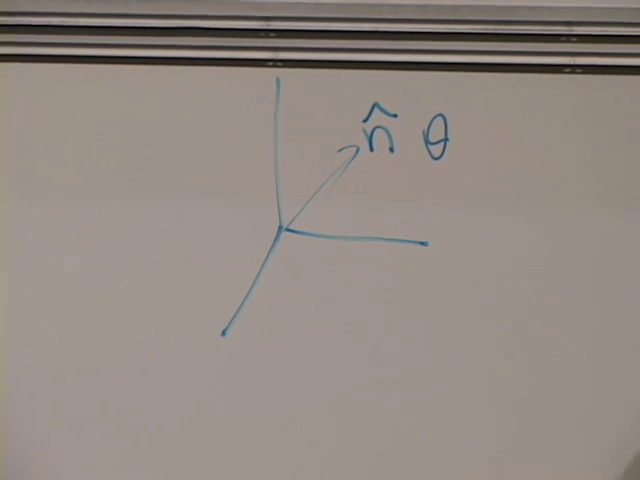
\includegraphics[width=0.58\textwidth]{lecture_03_figure_02.png}
\caption{회전축 \(\hat{\boldsymbol n}\)과 각도 \(\theta\)이 공간 회전을 정한다.}
\lectureframe{00:02:34}
\end{figure}

단위 구면 위의 방향은 경도와 위도처럼 두 매개변수로 정할 수 있다. 그 방향을 축으로 하는 회전각이 세 번째 매개변수다. 따라서 회전은 세 매개변수로 이루어진 족을 이룬다. 각도가 \(2\pi\)만큼 차이 날 때 생기는 전역적 동일시 문제는 아직 고려하지 않겠다. 여기서는 국소적인 매개변수의 개수가 중요하다.

축-각도 표현에는 중복이 있다. 축의 방향과 각도의 부호를 함께 뒤집어도 같은 연산이고, 충분히 큰 각도는 한 바퀴를 기준으로 줄일 수 있다. 그래도 항등원 근처에서 회전이 연속적으로 변하는 매개변수 세 개를 가진다는 사실은 달라지지 않는다. 이 국소적인 개수는 나중에 행렬 표현의 독립 매개변수 개수와 대응시킬 것이다.

이제 군의 성질을 차례로 확인할 수 있다:
\begin{enumerate}
\item \emph{닫힘.} 회전을 연이어 두 번 하면 또 다른 회전이 된다.
\item \emph{항등원.} 아무것도 하지 않는 것이 항등 회전이다.
\item \emph{역원.} \(\hat{\boldsymbol n}\)을 축으로 \(\theta\)만큼 회전한 것은 같은 축을 중심으로 \(-\theta\)만큼 회전하면 되돌릴 수 있다.
\item \emph{결합법칙.} 회전 세 번을 연이어 하면 다음이 성립한다.
\[
(R_1R_2)R_3=R_1(R_2R_3).
\]
\end{enumerate}

회전은 교환법칙을 따르지 않는다. \(x\)축을 중심으로 회전한 다음 \(y\)축을 중심으로 회전하면, 일반적으로 같은 두 연산을 역순으로 했을 때와 방향이 달라진다:
\begin{equation}
R_x(\alpha)R_y(\beta)\ne R_y(\beta)R_x(\alpha).
\end{equation}
두 각도가 모두 매우 작으면 차이는 2차항부터 나타나므로 무한소 회전은 거의 교환하는 것처럼 보일 수 있다. 그렇지만 전체 군은 비가환군이다.

어떤 방정식도 쓰지 않고 비가환성을 확인할 수 있다. 책이나 상자를 가져와 한 면을 앞면으로 표시한 뒤, \(x\)축을 중심으로 90도 회전하고 이어서 \(y\)축을 중심으로 90도 회전해 보자. 처음 방향으로 되돌아가 회전 순서를 바꾸어도 같은 동작을 해 보자. 표시한 면은 서로 다른 방향을 향하게 된다. 각도가 작으면 차이를 알아보기 어렵지만, 차이가 사라진 것은 아니다. 두 작은 각도의 곱에서 시작한다.

\begin{classroomqa}
\audiencequestion{이 회전들은 동시에가 아니라 차례로 하는 건가요?\lecturetimestamp{00:04:45}}
\lecturerresponse{그렇습니다. 군의 곱셈은 한 연산을 한 다음 다른 연산을 하는 것을 뜻합니다. 바로 이 연속된 회전들의 순서 때문에 교환법칙이 성립하지 않을 수 있습니다.}
\end{classroomqa}

이것이 우리가 처음 만나는 비가환군이다. 여기서 궁극적으로 다룰 대상은 보통 물체의 색이 아니라 쿼크의 빨강, 초록, 파랑 색 상태다. 이는 세 상태를 가진 내부 계이며, 흥미로운 변환은 세 색을 서로 섞는다. 보통의 회전은 연속군이 행렬을 통해 작용하는 방식을 보여 주는 친숙한 본보기다.

군 자체는 추상적이다. 물리학에서 군을 쓰려면 어떤 대상에 작용하는지 말해야 한다. {표현}은 각 군 원소에 연산자나 행렬을 대응시켜 군 원소의 곱셈이 대응하는 행렬들의 곱셈으로 재현되도록 한다. 서로 다른 물리적 대상은 같은 군의 서로 다른 표현을 가질 수 있다. 벡터, 스핀 1 상태, 스핀 1/2 상태가 세 가지 예가 될 것이다.

\section{3차원 벡터 표현}

보통의 벡터 성분을 다음과 같이 쓰자.
\begin{equation}
\boldsymbol V=(V_x,V_y,V_z),\qquad V_i,\quad i=1,2,3.
\end{equation}
좌표축을 고정한 채 물리적 벡터를 회전시킬 수도 있고, 벡터를 고정한 채 좌표축을 회전시킬 수도 있다. 두 방식의 규약은 다르지만 어느 쪽이든 성분은 \(3\times3\) 행렬에 의해 서로 섞인다. 축-각도 쌍 \((\hat{\boldsymbol n},\theta)\)마다 다음과 같이 쓰자.
\begin{equation}
V_i'=R_{ij}(\hat{\boldsymbol n},\theta)V_j,
\label{eq:l3-vector-rotation}
\end{equation}
여기서 반복된 첨자는 합산한다.

반복된 첨자 \(j\)는 더미 첨자다. 식~\eqref{eq:l3-vector-rotation}은 각 출력 성분 \(i\)에 대해 다음을 뜻한다.
\begin{equation}
V_i'=R_{i1}V_1+R_{i2}V_2+R_{i3}V_3
\end{equation}
자유 첨자 \(i\)는 계산할 성분을 표시하고, 반복된 첨자 \(j\)는 합산하며 식을 바꾸지 않고 이름을 바꿀 수 있다. 이 두 역할을 구분하면 길이 보존 논증에서 발생하는 대부분의 첨자 오류를 막을 수 있다.

\begin{figure}[htbp]
\centering
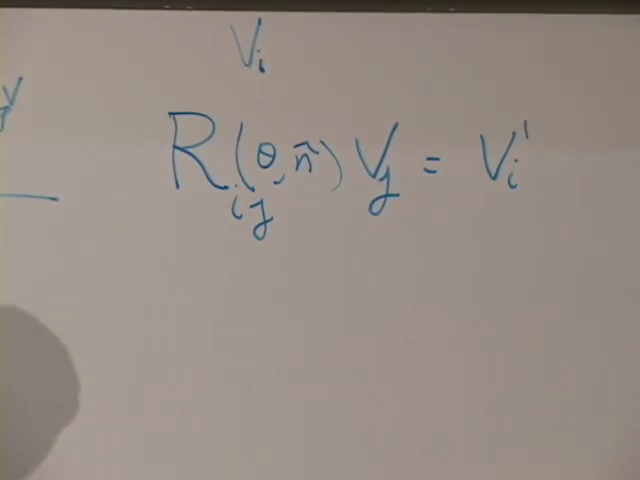
\includegraphics[width=0.68\textwidth]{lecture_03_figure_03.png}
\caption{회전 행렬은 원래 벡터 성분을 회전된 벡터 성분으로 사상한다.}
\lectureframe{00:07:41}
\end{figure}

참된 회전은 길이를 보존한다. 우선 \(V_i\)와 \(R_{ij}\)가 모두 실수이므로 다음이 성립한다.
\begin{equation}
V_i'V_i'=V_iV_i
\end{equation}
이는 모든 벡터에 대해 성립한다. 행렬 조건을 드러내기 위해 같은 변환을 더미 첨자를 달리해 쓰면 다음과 같다.
\begin{equation}
V_i'=R_{ij}V_j,\qquad V_i'=R_{ik}V_k.
\end{equation}
\(i\)에 대해 곱한 뒤 합하면 다음을 얻는다.
\begin{align}
V_i'V_i'
 &=R_{ij}V_jR_{ik}V_k\\
 &=R_{ij}R_{ik}V_jV_k.
\end{align}
이는 \(V_jV_j\)와 같아야 한다. 이 등식이 \(V\)의 모든 값에 대해 성립하려면 다음 조건이 필요하다.
\begin{equation}
R_{ij}R_{ik}=\delta_{jk}.
\label{eq:l3-orthogonality-index}
\end{equation}
행렬 표기법으로는
\begin{equation}
R^TR=\boldsymbol 1,
\label{eq:l3-orthogonal}
\end{equation}
따라서
\begin{equation}
R^{-1}=R^T.
\end{equation}
전치하면 행과 열이 서로 바뀐다.

계수가 왜 \(\delta_{jk}\)여야 할까? 크로네커 델타는 합산에서 \(j=k\)을 지정한다.
\begin{equation}
\delta_{jk}V_jV_k=V_1^2+V_2^2+V_3^2.
\end{equation}
\(R_{ij}R_{ik}\)가 \(\delta_{jk}\)와 다르면 어떤 방향이나 교차항 \(V_jV_k\)가 길이를 바꾸게 된다. 등식은 임의로 택한 한 벡터만이 아니라 가능한 모든 벡터에 대해 성립해야 하므로 행렬의 계수 자체가 항등행렬이어야 한다.

식~\eqref{eq:l3-orthogonal}은 이 실수 행렬 표현을 정의하는 직교 조건이다. 행렬을 곱하면 공간 회전의 곱셈표가 재현된다. 회전군의 표현이 이것뿐인 것은 아니다. 단지 가장 쉽게 시각화할 수 있는 표현이다.

역원 관계는 즉각적인 기하학적 의미를 갖는다. 새로운 행렬 방정식을 풀지 않고도 행과 열을 맞바꾸면 회전을 되돌릴 수 있다. \(R_1\)와 \(R_2\)가 두 회전을 나타낸다면, \(R_2R_1\)는 두 회전이 차례로 작용한 결과를 나타내며 역시 직교 행렬이다. 따라서 행렬 연산은 기하학적으로 확립한 닫힘, 항등원, 역원, 결합법칙의 구조를 그대로 보존한다.

\section{스핀 1과 벡터 표현}

이 3차원 표현은 양자 상태에도 작용한다. 스핀 1 입자는 다음과 같이 세 가지 스핀 투영값을 갖는다.
\begin{equation}
m=+1,\quad 0,\quad -1.
\end{equation}
따라서 스핀 상태는 확률진폭 세 개로 이루어진 열벡터다. 입자를 회전시키거나 스핀 축을 정의하는 데 쓰는 자기장의 방향을 바꾸면, 회전군의 3차원 표현에 의해 세 진폭이 서로 섞인다.

스핀 상태의 개수는 익숙한 규칙 \(2s+1\)을 따른다. 스핀 0에는 상태가 하나, 스핀 1/2에는 둘, 스핀 1에는 셋, 스핀 3/2에는 넷이 있다. 따라서 상태 벡터의 차원은 스핀에 따라 달라진다. 같은 물리적 회전도 서로 다른 상태 공간에 작용할 때는 크기가 다른 행렬로 표현되어야 한다.

스핀 1 입자에 대해 다음 기저를 택하자.
\begin{equation}
\lvert 1,+1\rangle,qquad
\lvert 1,0\rangle,qquad
\lvert 1,-1\rangle.
\end{equation}
상태는 다음과 같다.
\begin{equation}
\lvert\psi\rangle
=c_{+}\lvert1,+1\rangle+c_0\lvert1,0\rangle+c_{-}\lvert1,-1\rangle.
\end{equation}
장치를 회전시켜도 네 번째 스핀 상태가 생기지는 않는다. 계수 \(c_+,c_0,c_-\)가 서로 섞일 뿐이다. 따라서 이에 대응하는 회전 연산자는 \(3\times3\) 행렬이어야 한다.

스핀 1에서 이 표현은 보통의 공간 벡터와 같은 방식으로 변환된다. 스핀 1 입자를 \emph{벡터 입자}라고 부르는 정확한 의미는 이것이다. 스핀 진폭 세 개와 벡터 성분 세 개가 같은 회전 법칙을 따른다. 양자 상태를 실제 화살표라고 상상할 필요는 없다. 이는 성분들이 서로 섞이는 방식에 관한 설명이다.

이 대응은 우연이 아니다. 3차원 벡터와 스핀 1 상태는 회전군의 동등한 3차원 표현을 따른다. {벡터 입자}라는 말은 그러한 변환 성질을 요약한다. 양자 편광 상태가 입자 안에 숨은 작은 강체 화살표라고 주장하는 것은 아니다.

\section{이산 대칭과 연속 대칭}

스핀 1/2로 넘어가기 전에 두 가지 넓은 종류의 군을 구분하면 도움이 된다. 반사는 간단한 이산적 예다. 항등원이 있고 반사 \(P\)가 있다. 뒤집거나 뒤집지 않거나 둘 중 하나다. 반면 위상 \begin{equation}
e^{i\phi}
\end{equation}는 \(\phi\)에 따라 연속적으로 달라지고, 공간 회전은 축과 각도에 따라 연속적으로 달라진다. 이런 연속군을 Sophus Lie의 이름을 따서 \emph{리 군}이라 부르며, 이름은 \emph{리}라고 발음한다. 여기서는 연속 대칭을 주로 다루겠지만, 이산 대칭도 여전히 중요하다.

두 원소로 이루어진 반사군에서는
\begin{equation}
P^2=1.
\end{equation}
\(1\)와 \(P\) 사이에 연속적으로 조절할 수 있는 반사 정도는 없다. 위상군은 다르다. \(e^{i\phi_1}\)와 \(e^{i\phi_2}\) 사이에는 연속적으로 무한히 많은 다른 위상이 있다. 공간 회전도 같은 연속적 성질을 가지지만, \(U(1)\)와 달리 비가환군이다.

스핀 0은 회전군의 가장 간단한 표현을 제공한다. 스핀 0 상태는 모든 회전에 변하지 않으므로 각 군 원소는 1차원 항등원으로 표현된다.
\begin{equation}
D^{(0)}(R)=1.
\end{equation}
군 자체에는 여전히 회전이 무한히 많다. 자명한 것은 스핀 0 상태에 대한 표현이다.

군과 그 군의 표현 중 하나를 구분하는 것이 핵심이다. 회전군이 스칼라에 작용한다고 해서 군 자체가 원소 하나짜리 군으로 줄어드는 것은 아니다. 그저 특정 스칼라 상태에서는 모든 회전군 원소가 같은 수 \(1\)로 표현될 뿐이다.

\section{일반적인 스핀 1/2 상태}

스핀 1/2 계에는 기저 상태가 두 개 있다. 선택한 \(z\)축을 기준으로 하면
\begin{equation}
\lvert\uparrow\rangle=
\begin{pmatrix}1\\0\end{pmatrix},
\qquad
\lvert\downarrow\rangle=
\begin{pmatrix}0\\1\end{pmatrix}.
\end{equation}
일반적인 상태는 2성분 스피너다.
\begin{equation}
\lvert\psi\rangle=
\begin{pmatrix}\alpha_1\\\alpha_2\end{pmatrix},
\qquad
|\alpha_1|^2+|\alpha_2|^2=1.
\label{eq:l3-spinor}
\end{equation}
성분은 복소수다. \((\alpha_1,\alpha_2)=(1,0)\)은 스핀 업이고, \((0,1)\)는 스핀 다운이다. 정규화된 일반적인 선형결합은 다른 방향으로 편극된 스핀을 나타낸다.

{위}와 {아래}라는 말은 축을 정한 뒤에야 의미가 있다. 여기서 그 축은 \(z\)다. 측정축을 달리하면 기저 상태 쌍도 달라지며, 한 축을 따라 업 상태가 확정된 상태도 일반적으로 다른 기저에서는 중첩으로 나타난다. 물리적 스핀을 회전시키거나 기준 좌표축을 회전시키면 이에 따라 계수도 달라진다.

복소 진폭 두 개에는 실수 매개변수가 네 개 들어 있다. 정규화 조건으로 하나가 정해지고, 물리적으로 무관한 전체 위상으로 또 하나가 정해지므로 실수 매개변수 두 개가 남는다. 이는 구면 위의 방향을 정하는 데 필요한 개수와 정확히 같다. 회전을 연구하기 위해 \((\alpha_1,\alpha_2)\)와 그 방향 사이의 명시적인 대응 관계까지 유도할 필요는 없다.

전체 위상을 제거하는 이유는
\begin{equation}
\begin{pmatrix}\alpha_1\\\alpha_2\end{pmatrix}
\quad\hbox{and}\quad
e^{i\chi}
\begin{pmatrix}\alpha_1\\\alpha_2\end{pmatrix}
\end{equation}
가 같은 물리적 광선을 나타내기 때문이다. 정규화는 전체 확률을 정할 뿐, 보통의 유클리드 공간에서 방향을 정하는 것은 아니다. 이 두 가지 동일시를 적용하고 나면 남은 두 매개변수는 스핀 편극 방향의 극각과 방위각으로 볼 수 있다.

스핀을 회전시키면 상태는 다음과 같이 변한다.
\begin{equation}
\alpha_i'=U_{ij}\alpha_j,
\qquad
\begin{pmatrix}\alpha_1'\\\alpha_2'\end{pmatrix}
=
\begin{pmatrix}
U_{11}&U_{12}\\
U_{21}&U_{22}
\end{pmatrix}
\begin{pmatrix}\alpha_1\\\alpha_2\end{pmatrix}.
\label{eq:l3-spinor-transform}
\end{equation}
따라서 공간 회전은 스피너에 작용하는 2차원 행렬 표현을 갖는다. 이 표현에는 전역적으로 두 겹으로 대응하는 성질이 있지만, 이에 대한 논의는 뒤로 미루겠다. 국소적으로 이 행렬들은 아래에서 필요한 변환 성질을 갖는다.

변환된 쌍 \((\alpha_1',\alpha_2')\)도 가능한 양자 상태여야 한다. 따라서 \(U\)에 관해 먼저 물을 것은 명시적인 축-각도 공식이 아니라 모든 입력 스피너의 정규화를 보존하는 조건이다.

\section{확률 보존과 유니터리 행렬}

회전은 정규화된 상태를 또 다른 정규화 상태로 보내야 한다.
\begin{equation}
\alpha_i^*\alpha_i=\alpha_i'^*\alpha_i'=1.
\end{equation}
식~\eqref{eq:l3-spinor-transform}을 대입하면
\begin{align}
\alpha_i'^*\alpha_i'
 &=(U_{ij}\alpha_j)^*(U_{ik}\alpha_k)\\
 &=\alpha_j^*U_{ij}^*U_{ik}\alpha_k.
\end{align}
실수 벡터 조건에 대응하는 조건은 다음과 같다.
\begin{equation}
(U^T)^*U=\boldsymbol 1.
\end{equation}
전치한 뒤 복소켤레를 취한 것은 에르미트 켤레이며,
\begin{equation}
U^\dagger=(U^T)^*,
\end{equation}
따라서 정규화를 보존하는 조건은
\begin{equation}
U^\dagger U=\boldsymbol 1.
\label{eq:l3-unitarity}
\end{equation}

실수 벡터 계산과 본질적으로 달라지는 점은 복소켤레를 추가한다는 것뿐이다. 실수 벡터에서는 \(V_iV_i\)가 길이다. 스피너에서는 \(\alpha_i^*\alpha_i\)가 확률이다. 확률을 실수이자 음이 아닌 값으로 만들려면 복소켤레가 필요하므로, 전치 대신 에르미트 켤레를 쓴다.

식~\eqref{eq:l3-unitarity}에서 역원도 바로 얻을 수 있다.
\begin{equation}
U^{-1}=U^\dagger.
\end{equation}
따라서 역회전도 같은 확률 노름을 보존한다. 보통의 회전 행렬과 마찬가지로 유니터리 행렬들의 곱은 여전히 유니터리이므로, 이 표현은 군의 곱셈을 그대로 반영한다.

\begin{figure}[htbp]
\centering
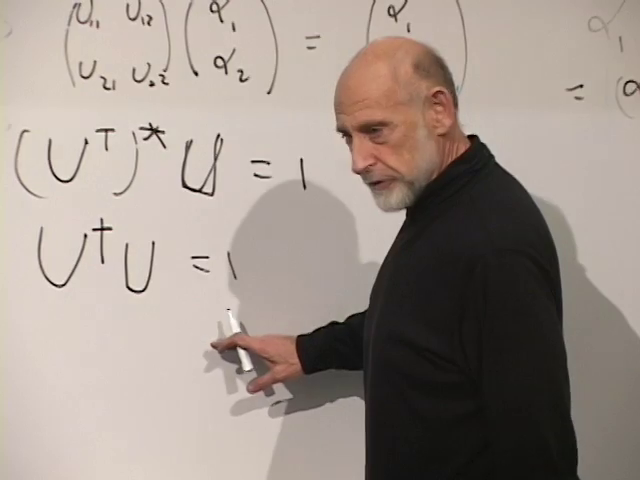
\includegraphics[width=0.62\textwidth]{lecture_03_figure_04.png}
\caption{스피너 회전 행렬은 \(U^\dagger U=\boldsymbol 1\)을 만족한다.}
\lectureframe{00:27:41}
\end{figure}

식~\eqref{eq:l3-unitarity}을 만족하는 행렬은 유니터리 행렬이다. 일반적인 \(2\times2\) 복소 행렬은 실수 매개변수 여덟 개로 시작한다. 유니터리 조건은 \(2\times2\) 행렬 방정식으로, 독립적인 실수 조건 네 개를 제공하므로 매개변수 네 개가 남는다. 공간 회전의 매개변수는 세 개뿐이다. 스피너의 회전 표현을 \(U(2)\) 전체에서 골라내려면 조건이 하나 더 필요하다.

두 열을 복소 벡터 두 개로 보면 조건 네 개를 확인할 수 있다. \(U\)의 각 열은 단위 노름을 가져야 하므로 실수 조건 두 개가 생기고, 두 열은 서로 직교해야 하므로 복소 조건 하나, 즉 실수 조건 두 개가 생긴다. 모두 합해 네 개다. \(U(2)\)에 남은 네 번째 매개변수는 새로운 공간 회전이 아니라 전체 행렬식 위상으로 밝혀질 것이다.

\section{행렬식 1과 \texorpdfstring{\(SU(2)\)}{SU(2)}}

추가 조건은 다음과 같다.
\begin{equation}
\det U=1.
\label{eq:l3-det-one}
\end{equation}
이 조건은 군의 곱셈과 양립한다. 왜냐하면
\begin{equation}
\det(AB)=\det A\,\det B.
\end{equation}
행렬식이 1인 유니터리 행렬 두 개를 곱해도 행렬식은 1이고, 항등행렬의 행렬식도 1이다. 이 행렬들은 닫힌 부분군을 이룬다.

역원도 이 부분군에 속한다. \(\det U=1\)이면 다음과 같다.
\begin{equation}
\det U^{-1}=\frac{1}{\det U}=1.
\end{equation}
따라서 행렬식 1 조건을 부과해도 항등원이 빠지거나 닫힘이 깨지거나 역원이 사라지지 않는다. 이 조건은 연속 매개변수가 하나 적은 군을 일관되게 선택한다.

유니터리 조건만으로도 다음이 성립한다.
\begin{equation}
\det(U^\dagger U)=
(\det U)^*\det U
=|\det U|^2=1.
\end{equation}
하지만 이 조건만으로 \(\det U\)가 \(+1\) 또는 \(-1\)이 되도록 강제되지는 않는다. 일반적인 유니터리 행렬의 행렬식은 임의의 위상일 수 있다.
\begin{equation}
\det U=e^{i\phi},
\qquad
\det U^\dagger=e^{-i\phi}.
\end{equation}
조건~\eqref{eq:l3-det-one}은 이 자유 위상을 고정해 실수 매개변수 하나를 제거한다.

\begin{classroomqa}
\audiencequestion{\(U^\dagger U=\boldsymbol 1\)만으로 \(\det U^\dagger\)가 \(\det U\)와 같거나 오직 \(+1\) 또는 \(-1\)만 되도록 강제되나요?\lecturetimestamp{00:31:21}}
\lecturerresponse{아닙니다. 두 행렬식은 서로 복소켤레입니다. 둘은 \(e^{i\phi}\)와 \(e^{-i\phi}\)일 수 있고, 이들의 곱은 1입니다. 특수 유니터리 조건을 부과하면 두 행렬식 모두 1로 고정됩니다.}
\end{classroomqa}

\(n\times n\) 행렬로 이루어진 유니터리군은 \(U(n)\)이다. \(n=1\)일 때 유니터리 행렬은 위상 \(e^{i\phi}\) 하나이므로 \(U(1)\)이 된다. 행렬식이 1인 부분군은 \emph{특수 유니터리군}이라 하며,
\begin{equation}
SU(n)=\{U\in U(n):\det U=1\}.
\end{equation}
2성분 스피너에는 3매개변수 군인 \(SU(2)\)가 작용한다.

표기법은 두 조건을 모두 나타낸다. \(U\)는 유니터리임을, \(S\)는 특수, 즉 행렬식이 1임을 뜻한다. 특수 유니터리군은 복소 내적을 보존하면서 행렬식에 실리는 독립적인 공통 위상을 배제하므로 여러 곳에서 반복해서 등장한다.

국소적으로 \(SU(2)\)는 스핀 1/2 상태를 회전시키는 데 필요한 회전 대수와 곱셈 구조를 가진다. 전역적으로는 앞서 미룬 세부 사항을 기억해야 한다. \(SU(2)\)는 보통의 회전군 \(SO(3)\)의 이중 덮개이므로, \(SU(2)\)의 원소 두 개가 공간 회전 하나에 대응한다. \editorialnote{이중 덮개라는 정식화는 원문에서 언급만 하고 전개하지 않은 두 겹 대응을 엄밀히 나타낸다.}

\section{무한소 회전과 파울리 행렬}

\begin{classroomqa}
\audiencequestion{스핀 행렬, 즉 파울리 행렬은 이 구성의 어디에서 등장하나요?\lecturetimestamp{00:33:16}}
\lecturerresponse{군 원소를 항등원에 아주 가까이, 즉 회전각이 매우 작은 경우로 두면 등장합니다. 이들은 그런 무한소 회전의 생성자입니다.}
\end{classroomqa}

다음과 같이 두자.
\begin{equation}
U=\boldsymbol 1+\epsilon M+O(\epsilon^2),
\label{eq:l3-small-u-anti}
\end{equation}
여기서 \(\epsilon\)는 실수이며 작다. 그러면
\begin{equation}
U^\dagger=\boldsymbol 1+\epsilon M^\dagger+O(\epsilon^2),
\end{equation}
유니터리 조건으로부터
\begin{align}
U^\dagger U
 &=\boldsymbol 1+\epsilon(M^\dagger+M)+O(\epsilon^2).
\end{align}
1차까지 보면
\begin{equation}
M^\dagger=-M.
\end{equation}
따라서 식~\eqref{eq:l3-small-u-anti}의 행렬 \(M\)은 반에르미트 행렬이다.

여기서는 \(\epsilon\)에 비례하는 항만 남긴다. 곱 \(\epsilon^2M^\dagger M\)은 2차항이므로 버린다. 항등원 가까이에서 다루면 비선형 군 조건이 생성자에 대한 선형 조건으로 바뀐다는 것이 이 방법의 장점이다.

\(i\)를 묶어내는 편이 더 편리하다.
\begin{equation}
U=\boldsymbol 1+i\epsilon H+O(\epsilon^2).
\label{eq:l3-small-u-herm}
\end{equation}
복소켤레를 취하면 \(i\)가 \(-i\)로 바뀌므로
\begin{equation}
U^\dagger=\boldsymbol 1-i\epsilon H^\dagger+O(\epsilon^2).
\end{equation}
이제
\begin{equation}
U^\dagger U
=\boldsymbol 1+i\epsilon(H-H^\dagger)+O(\epsilon^2),
\end{equation}
1차 유니터리 조건은 다음을 요구한다.
\begin{equation}
H^\dagger=H.
\end{equation}
\(i\)를 묶어내면 생성자가 에르미트 행렬이 된다.

\(i\)를 곱해도 허용되는 무한소 행렬은 달라지지 않았다. 생성자에 이름을 붙이는 규약만 달라졌다. 물리학에서는 고유값이 실수이고 각운동량 같은 관측량이 에르미트 연산자이므로 보통 에르미트 생성자를 택한다.

행렬식이 1이라는 조건은 무추적성\editorialnote{말로 행렬식을 전개한 대목에서 첨자가 잠시 잘못 언급되었다. 올바른 선형항은 \(A_{11}+A_{22}=\operatorname{tr}A\)이다. 비대각 원소들의 곱은 2차항부터 나타난다.}을 부과한다. 작은 \(2\times2\) 행렬 \(A\)에 대해
\begin{equation}
\det(\boldsymbol 1+A)
=
\det
\begin{pmatrix}
1+A_{11}&A_{12}\\
A_{21}&1+A_{22}
\end{pmatrix}.
\end{equation}
전개하면
\begin{align}
\det(\boldsymbol 1+A)
 &=(1+A_{11})(1+A_{22})-A_{12}A_{21}\\
 &=1+A_{11}+A_{22}+O(A^2)\\
 &=1+\operatorname{tr}A+O(A^2).
\end{align}
이를 \(A=i\epsilon H\)에 적용하면
\begin{equation}
\det U=1+i\epsilon\,\operatorname{tr}H+O(\epsilon^2).
\end{equation}
따라서 \(\det U=1\)이면 다음을 만족해야 한다.
\begin{equation}
\operatorname{tr}H=0.
\end{equation}
추적 조건은 항등행렬에 비례하는 생성자를 정확히 제거한다. 일반적인 에르미트 \(2\times2\) 행렬에는 실수 대각 성분 두 개와 복소 비대각 성분 하나, 모두 네 개의 실수 매개변수가 있다. 추적 조건은 실수 조합 하나를 고정하므로 세 개가 남는다. 이는 무한소 공간 회전을 할 수 있는 세 축의 개수와 일치한다.

따라서 \(SU(2)\)의 무한소 생성자는 무추적 에르미트 \(2\times2\) 행렬이다. 파울리 행렬 세 개가 기저를 이룬다.
\begin{equation}
\begin{aligned}
\sigma_x&=
\begin{pmatrix}0&1\\1&0\end{pmatrix},
&
\sigma_y&=
\begin{pmatrix}0&-i\\i&0\end{pmatrix},
\\[0.4em]
\sigma_z&=
\begin{pmatrix}1&0\\0&-1\end{pmatrix}.
\end{aligned}
\end{equation}
모든 생성자는 다음과 같이 쓸 수 있다.
\begin{equation}
H=a_x\sigma_x+a_y\sigma_y+a_z\sigma_z.
\end{equation}
\(x\)축을 중심으로 한 작은 회전에는 \(\sigma_x\)가, \(y\)축을 중심으로 한 작은 회전에는 \(\sigma_y\)가 선택된다. 다른 축을 중심으로 회전하면 이에 대응하는 선형결합이 선택된다. \(\hbar=1\)인 단위계에서 스핀 연산자는 다음과 같다.
\begin{equation}
S_i=\frac{\sigma_i}{2}.
\end{equation}

예를 들어 \(x\)축과 \(y\)축의 중간 방향에 해당하는 생성자는 다음에 비례한다.
\begin{equation}
\frac{\sigma_x+\sigma_y}{\sqrt2}.
\end{equation}
계수 벡터의 방향 \((a_x,a_y,a_z)\)가 회전축을 정하고, 그 크기와 \(\epsilon\)가 함께 작은 회전각을 정한다. 이것이 각운동량 교환자에서 등장하는 스핀 행렬과 유한 회전 연산자의 관계다. 특히
\begin{equation}
[S_x,S_y]=iS_z
\end{equation}
그리고 순환적으로 첨자를 바꾼 관계들이 기하학적으로 확인한 비가환성을 나타낸다. 무한소 생성자를 지수화하면 표준적인 유한 회전을 얻는다.\editorialnote{유한 회전의 지수함수 공식은 무한소 구성의 표준적인 완성형이다. 원문에서는 생성자 조건과 파울리 행렬 기저만 유도한다.},
\begin{equation}
U(\hat{\boldsymbol n},\theta)
=\exp\left(-\frac{i\theta}{2}\,
\hat{\boldsymbol n}\cdot\boldsymbol\sigma\right).
\end{equation}
\section{세 상태 색 공간}

표현들을 결합하는 일은 나중에 다루기로 하자. 이제 공간 스핀을 떠나 쿼크의 색으로 돌아간다. 쿼크의 스핀은 여전히 1/2이지만, 색은 그와 독립적인 세 상태 자유도다.
\begin{equation}
\lvert r\rangle,\qquad
\lvert g\rangle,\qquad
\lvert b\rangle.
\end{equation}
일반적인 색 상태는 다음과 같다.
\begin{equation}
\begin{aligned}
\lvert q\rangle_{\mathrm{color}}
={}&
\alpha_r\lvert r\rangle
+\alpha_g\lvert g\rangle
+\alpha_b\lvert b\rangle,
\\
&|\alpha_r|^2+|\alpha_g|^2+|\alpha_b|^2=1.
\end{aligned}
\end{equation}
이를 다음과 같이 쓸 수도 있다.
\begin{equation}
q=
\begin{pmatrix}
\alpha_r\\
\alpha_g\\
\alpha_b
\end{pmatrix}.
\end{equation}
제곱한 절댓값은 선택한 색 기저에서 빨강, 초록, 파랑일 확률이다. 같은 삼중항 표기로 쿼크 장 연산자 세 개를 모아 다음처럼 쓸 수 있다.
\begin{equation}
\psi=
\begin{pmatrix}
\psi_r\\
\psi_g\\
\psi_b
\end{pmatrix}.
\end{equation}

스핀과 색은 개념적으로 구분해야 한다. 스핀 표지는 상태가 물리적 공간의 회전에 어떻게 변환되는지 나타낸다. 색 표지는 실험실을 회전시키지 않는 내부 대칭에 따라 상태가 어떻게 변환되는지 나타낸다. 쿼크 상태는 두 표지를 모두 가지지만, 여기서는 색에 집중하기 위해 스핀은 생략한다.

장 연산자 세 개를 한 열에 쓰는 것은 단순한 정리 방식 이상의 의미가 있다. 이로써 대칭을 하나의 행렬 방정식으로 표현할 수 있다. 공간 회전이 한 벡터 성분을 다른 성분들의 선형결합으로 바꾸듯, 변환에 따라 빨강 장이 빨강, 초록, 파랑 장의 선형결합으로 바뀔 수 있다.

먼저 두 색을 맞바꾸는 이산 변환을 생각해 볼 수 있다. 더 큰 대칭군에는 세 색 모두를 연속적으로 섞는 변환이 포함된다. 단순한 색 교환 행렬은 행렬식이 1이 되도록 위상을 곱해 주어야 할 수 있다. 이렇게 위상을 곱하면 그 교환은 특수 유니터리군 안에 포함된다.

기저 상태 두 개를 그대로 맞바꾸는 변환은 다음 행렬로 나타난다.
\begin{equation}
X=
\begin{pmatrix}0&1\\1&0\end{pmatrix},
\qquad
\det X=-1.
\end{equation}
행렬 전체에 \(i\)를 곱하면 다음을 얻는다.
\begin{equation}
\det(iX)=i^2\det X=1.
\end{equation}
따라서 위상을 일관되게 정하면 이산적인 교환도 더 큰 연속군의 특정 원소로 나타낼 수 있다.

\begin{classroomqa}
\audiencequestion{기저 상태 두 개만 맞바꾸는 행렬은 행렬식이 잘못되어 \(SU(2)\)에 속하지 못하나요?\lecturetimestamp{00:43:46}}
\lecturerresponse{그대로 맞바꾸는 행렬의 행렬식은 \(-1\)입니다. 적절한 \(i\) 인자를 곱하면 행렬식이 1인 대표 원소를 얻을 수 있으므로, 이 교환도 연속적인 특수 유니터리 변환에 포함할 수 있습니다.}
\end{classroomqa}

\section{\texorpdfstring{\(SU(3)\)}{SU(3)}과 여덟 개의 색 생성자}

연속적인 색 변환은 다음과 같다.
\begin{equation}
\begin{aligned}
q'&=Uq,
&
U^\dagger U&=\boldsymbol 1,
\\
\det U&=1,
&
U&\in SU(3).
\end{aligned}
\label{eq:l3-su3-action}
\end{equation}
수학적 구성은 스피너에 사용한 특수 유니터리 구성과 같지만, 이제 \(U\)는 \(3\times3\)이다. 이는 물리적 공간의 회전이 아니다. 내부 색 공간에서의 회전이다.

유니터리 조건은 색 상태의 정규화를 보존한다.
\begin{equation}
q^\dagger q
=|\alpha_r|^2+|\alpha_g|^2+|\alpha_b|^2.
\end{equation}
행렬식 1 조건은 연속적인 혼합에서 공통 \(U(1)\) 위상 방향을 제거한다. 이렇게 얻은 행렬들은 단순한 교환, 상대 위상 변화, 실제로 연속적인 중첩을 만들 수 있으며, 모두 하나의 닫힌 군에 속한다.

매개변수의 개수는 바로 알 수 있다. \(3\times3\) 복소 행렬에는 복소 성분이 아홉 개, 즉 실수 매개변수가 열여덟 개 있다. 행렬 방정식 \(U^\dagger U=\boldsymbol 1\)은 실수 조건 아홉 개를 부과한다. 행렬식 1 조건이 하나를 더 제거한다.
\begin{equation}
\dim SU(3)=18-9-1=8.
\end{equation}
따라서 \(SU(3)\)에는 독립적인 무한소 생성자가 여덟 개 있다.

유니터리 조건의 실수식 아홉 개는 \(U\)의 열을 보면 다시 이해할 수 있다. 복소 열 세 개는 각각 단위 노름을 가져야 하며, 모든 열 쌍은 서로 직교해야 한다. 이 조건들은 처음의 실수 매개변수 열여덟 개 중 아홉 개를 제거한다. 행렬식 위상이 하나를 더 제거해 여덟 개가 남는다. 이는 \(SU(2)\)의 \(8-4-1=3\)와 같은 방식으로 세 상태에 확장한 결과다.

여덟이라는 수가 나타난다는 사실은 결국 글루온 종이 여덟 개가 되는 것과 같은 사실이다. 행렬식 제한으로 한 방향이 제거되었기 때문에 글루온이 아홉 개가 아니라고 말하는 것은 기억을 돕기 위한 표현일 뿐이다. 더 정확히 말하면 아홉 개의 색-반색 행렬은 단위행렬에 비례하는 하나의 색 단일항 방향과 여덟 개의 무대각합 방향으로 분해된다. 이 여덟 무대각합 생성자가 QCD 글루온이 지니는 수반 색 구조를 이룬다.\editorialnote{단일항과 팔중항으로 구성하는 정식화는 원문에서 의도적으로 직관적으로 제시한 행렬식 관련 설명을 엄밀하게 표현한 표준적인 방식이다. 게이지 장의 구성은 뒤에서 다룬다.}

이 단계에서 글루온 여덟 개와의 관계는 앞으로 다룰 내용을 가리킬 뿐, 아직 완전한 유도는 아니다. 게이지 입자를 얻으려면 색 대칭을 국소 대칭으로 승격하고 이를 보상하는 장을 정해야 한다. 매개변수 개수로 이미 밝혀진 것은 \(SU(3)\) 색 변환이 항등원에서 벗어나기 시작할 수 있는 독립적인 방향이 여덟 개라는 점이다.

\section{색 대칭이 QCD를 제약한다}

기본적인 대칭성 진술은 식~\eqref{eq:l3-su3-action}의 색 변환 아래에서 물리가 불변이라는 것이다. 이는 양자색역학의 핵심적인 내부 대칭이다. 색 성분을 섞는 형식은 스핀 위와 스핀 아래의 진폭을 섞는 것과 유사하고, 이러한 스피너 변환은 다시 공간 방향의 회전과 관련되지만, 이 세 공간을 혼동해서는 안 된다.

색을 대칭이라고 하는 것은 색 기저를 바꾸어도 물리적 예측이 달라지지 않는다는 뜻이다. 빨강, 초록, 파랑은 세 기저 벡터를 편의상 부르는 이름이지, 관측 가능한 세 가지 안료가 아니다. 색 성분을 동시에 \(SU(3)\) 회전해도 법칙의 형태는 변하지 않아야 한다. 이 불변성은 선택적인 미적 요소가 아니라 QCD를 조직하는 원리다.

대칭성은 라그랑지안을 제약한다. 앞서 살펴본 \(U(1)\) 예에서는 공통 위상 변환에 대한 불변성으로 인해 장과 그 켤레의 인자가 균형을 이루는 항만 허용되었다. QCD에서도 모든 항은 \(SU(3)\) 색 변환에 대해 불변이어야 한다. 이 요구는 상호작용과 보존량, 글루온 장의 형태에 영향을 준다.

어떤 항이 드러난 색 지수를 가진다고 하자. 식~\eqref{eq:l3-su3-action}에 따르면 그 지수는 회전하므로, 그 항만으로는 불변일 수 없다. 허용되는 항은 색 지수를 불변 조합으로 수축하거나, 변환으로 인한 변화를 보상하는 게이지 장을 사용해야 한다. 이것이 대칭성 원리가 실제로 작용하는 방식이다. 임의의 결합을 배제하고 남는 상호작용을 체계화한다.

QCD를 완성하려면 한 단계가 더 필요하다. 색 변환이 점마다 달라질 수 있어야 하고, 게이지 장은 그 국소적인 변화를 보상해야 한다.\editorialnote{색 대칭을 국소화하는 것은 전역 \(SU(3)\) 대칭성 논의를 게이지 이론으로 완성하는 표준적인 방식이지만, 이 강의 원문에서는 전개하지 않는다.}그 전개는 다음 단계에서 다룬다. 지금은 핵심 구조가 갖추어졌다. 여덟 생성자를 갖는 특수 유니터리 3상태 대칭이 색 삼중항에 작용한다.

당장은 필요한 만큼 군론을 살펴보았다. 일상적인 공간에서 그릴 수 있는 회전에서 시작해 벡터와 스피너에 작용하는 행렬로 나아갔고, 이어 내부 색 공간에서 같은 논리를 다시 사용했다. 이제 수학적 틀을 갖춘 채 입자물리학으로 돌아갈 수 있다. 형식론에 물리적 설명 전체를 한꺼번에 떠맡길 필요는 없다.
\chapter{색 표현, 강입자, 그리고 가둠}

\paragraph{짧은 도입부.}
군론으로 돌아가기 전에 염치 불고하고 짧게 홍보 하나만 하겠습니다. \emph{블랙홀 전쟁}은 블랙홀이 양자 정보를 파괴하는지를 두고 스티븐 호킹과 오랫동안 논쟁한 이야기를 담고 있습니다. 이 책에는 이론물리학자 특유의 잔인함도 기록되어 있습니다. 슈뢰딩거의 고양이뿐 아니라 서스킨드의 물고기와 그 불운한 변기행까지 말입니다. 이 책무를 마쳤으니 앨리스와 밥으로 돌아갑시다. 밥이 여전히 앨리스에게 군론을 배우게 하고 있으니, 앨리스는 아직도 고생 중입니다.

\lectureoverview{대칭은 상태에 작용할 때 물리적 의미를 갖습니다. 먼저 회전을 이용해 표현과 생성자를 소개한 다음, 색 \(SU(3)\)에 대해서도 같은 구성을 살펴보겠습니다. 색 표현들이 결합해 강입자를 이루며, 그 동역학은 고립된 색이 관측되지 않는 이유를 설명합니다.}

\section{군과 군이 작용하는 대상}

대칭을 논할 때는 두 가지 개념이 있습니다. 첫째는 곱셈 법칙과 항등원, 역원을 갖는 연산들의 모임인 추상군입니다. 둘째는 그 연산들이 작용하는 대상입니다. 두 개념은 구분할 수 있지만, 물리학에서는 서로 떼어 놓을 수 없습니다. 대칭이 중요한 까닭은 물리적 상태, 장, 좌표 또는 관측량을 변환하기 때문입니다.

\begin{classroomqa}
\audiencequestion{군을 추상적인 곱셈표로 설명하기도 하고 물리적 대상에 작용하는 행렬로 설명하기도 했습니다. 이 두 부분을 분리할 수 있습니까?
\lecturetimestamp{00:01:58}}
\lecturerresponse{서로 다른 기술 수준이지만 완전히 연결되어 있습니다. 회전은 무엇을 회전시키는지 정하기 전에도 추상적 연산으로 존재합니다. 그런 다음 물리학에서는 같은 연산이 특정 계와 관련된 상태와 양에 어떻게 작용하는지 묻습니다. 행렬은 추상적인 곱셈 법칙을 보존하면서 그 작용을 구체적으로 나타냅니다.}
\end{classroomqa}

공간 회전이 가장 명료한 예입니다. 고전적으로 같은 회전은 입자의 좌표, 자석의 방향 또는 다른 벡터에 작용할 수 있습니다. 양자역학에서 상태는 선형 벡터 공간에 있으므로, 회전은 그 공간에 작용하는 선형 연산자로 표현됩니다. 추상군 원소를 \(g\), 그 행렬 표현을 \(D(g)\)라 하면, 일관성을 위해 다음이 성립해야 합니다.
\begin{equation}
D(g_1g_2)=D(g_1)D(g_2),
\qquad
D(e)=\boldsymbol 1.
\end{equation}
행렬이 추상적인 연산과 같은 모양일 필요는 없지만, 행렬의 곱셈은 군의 곱셈을 재현해야 합니다.
\editorialnote{준동형 방정식은 원문에서 말로 설명한 군 곱셈과 행렬 곱셈 사이의 대응을 명시적으로 나타냅니다.}

행렬의 차원은 추상군만으로 정해지는 것이 아니라 상태 공간으로 정해집니다. 전자 하나의 스핀만 고려하면 서로 직교하는 두 가지 가능성, 즉 스핀 위와 스핀 아래가 있고, 상태는 두 성분 열벡터입니다. 따라서 회전은 \(2\times2\) 행렬로 작용합니다. 스핀 1/2인 두 대상에는 네 가지 기저 상태가 있습니다.
\begin{equation}
\ket{\uparrow\uparrow},\qquad
\ket{\uparrow\downarrow},\qquad
\ket{\downarrow\uparrow},\qquad
\ket{\downarrow\downarrow},
\end{equation}
결합된 공간에서 유도되는 작용은 4차원입니다.

익숙한 순서는 다음과 같습니다.
\begin{equation}
\begin{array}{c|c|c}
\text{spin} & \text{number of states} & \text{matrix dimension}\\
\hline
0 & 1 & 1\times1\\
\frac12 & 2 & 2\times2\\
1 & 3 & 3\times3\\
\frac32 & 4 & 4\times4
\end{array}
\end{equation}
스핀 0 상태는 자명 표현을 이룹니다. 모든 회전이 이 상태를 그대로 둡니다. 1×1 행렬은 그저 \(1\)입니다. 스핀 1 상태에는 세 성분이 있으며, 그 회전 행렬은 익숙한 3차원 벡터 회전 행렬입니다. 더 일반적으로 스핀 \(j\)에는 \(2j+1\)개의 상태가 있습니다.

표현은 무한 차원일 수도 있습니다. 전자의 스핀만이 아니라 전체 궤도 운동을 기술하면, 상태에는 위치마다, 또는 동등하게 운동량마다 진폭이 있습니다. 그러면 회전 연산자는 무한 차원 파동함수 공간에 작용합니다. 따라서 하나의 추상 회전군이 자명 표현, 2차원 표현, 3차원 표현, 무한 차원 표현을 모두 가질 수 있습니다. 논의가 스핀에서 색으로 옮겨갈 때 이 사실을 다시 활용하겠습니다.

\section{스핀 회전이 특수 유니터리인 이유}

이제 전자 하나의 스핀으로 돌아가 궤도 운동은 제외합시다. 회전은 \(2\times2\) 유니터리 행렬 \(U\)로 표현됩니다.
\begin{equation}
U^\dagger U=\boldsymbol 1,
\qquad
U^{-1}=U^\dagger.
\label{eq:l4-unitarity}
\end{equation}
역변환은 회전을 되돌려야 하며, 유니터리성은 노름과 따라서 모든 확률을 보존합니다.

일반적인 \(2\times2\) 복소 행렬에는 복소 성분이 네 개, 즉 실수 매개변수가 여덟 개 있습니다. 식~\eqref{eq:l4-unitarity}은 서로 독립인 실수 조건 네 개를 부과하므로 매개변수 네 개가 남습니다. 보통의 공간 회전에는 매개변수가 세 개뿐입니다. 두 개는 회전축을 정하고 하나는 각도를 정합니다. 따라서 유니터리 행렬에는 위상이 하나 더 들어 있습니다. 추가 제약은 다음과 같습니다.
\begin{equation}
\det U=1.
\label{eq:l4-det-one}
\end{equation}
그러면 매개변수 개수는 다음과 같습니다.
\begin{equation}
8-4-1=3.
\end{equation}

행렬식이 1이라는 조건은 곱셈에 대해 보존된다.
\begin{equation}
\det(AB)=\det A\,\det B.
\end{equation}
행렬식이 각각 1인 두 행렬의 곱도 같은 조건을 만족하기 때문이다. 이 조건은 유니터리성과도 양립한다. ~\eqref{eq:l4-unitarity}의 양변에 행렬식을 취하면
\begin{equation}
1=\det(U^\dagger U)
=\det(U^\dagger)\det U
=(\det U)^*\det U.
\end{equation}
따라서 유니터리 행렬의 행렬식은 복소평면의 단위원 위에 놓인다.
\begin{equation}
\det U=e^{i\phi}.
\end{equation}

\begin{classroomqa}
\audiencequestion{유니터리성은 행렬식이 실수여야 한다는 뜻인가요?
\lecturetimestamp{00:12:10}}
\lecturerresponse{아닙니다. 유니터리성이 요구하는 것은 절댓값이 1이라는 조건뿐입니다. 행렬식은 임의의 순수 위상 \(e^{i\phi}\)일 수 있습니다. 2차원 행렬에서는 \(U\)에 \(e^{-i\phi/2}\)를 곱해 공통 위상을 없애면 행렬식이 1인 행렬을 얻습니다.}
\end{classroomqa}

실제로,
\begin{equation}
V=e^{-i\phi/2}U,
\end{equation}
이라면 \(V\)는 여전히 유니터리이고,
\begin{equation}
\det V=e^{-i\phi}\det U=1.
\end{equation}
행렬식이 1인 유니터리 행렬들은 \(SU(2)\)을 이룹니다.

여기에는 한 가지 세밀한 점이 있습니다. \(SU(2)\)가 3차원 공간의 회전군이라고만 말하고 싶겠지만, 대응은 두 대 일입니다. 행렬 \(U\)와 \(-U\)는 스피너에 서로 다르게 작용하지만, 보통의 벡터를 같은 회전으로 변환합니다. 따라서
\begin{equation}
SU(2)/\{\boldsymbol 1,-\boldsymbol 1\}\simeq SO(3).
\end{equation}
현재 논의에서는 국소적인 곱셈 구조와 세 생성자가 중요하지만, 이중 덮개 구조는 스핀 1/2 회전이 두 값을 갖는 이유를 설명합니다.

\section{무한소 변환과 그 생성자}

유한 회전은 아주 작은 회전들을 여러 번 적용해 만들 수 있습니다. 항등원에 가까운 군 원소를 무한소 원소라고 하며, 연결군에서는 모든 무한소 방향을 알면 반복적인 곱셈으로 유한 변환을 재구성하기에 충분합니다. 물리학에서 더 중요한 점은 이러한 무한소 변환을 생성하는 연산자가 대칭에 대응하는 보존량이라는 사실입니다.

항등원에 가까운 원소를 다음과 같이 씁니다.
\begin{equation}
U=\boldsymbol 1+i\epsilon T,
\qquad |\epsilon|\ll1.
\label{eq:l4-infinitesimal-u}
\end{equation}
\(i\) 인자는 편리한 약속입니다. 이를 유니터리 조건에 대입하고 \(\epsilon^2\) 차수 항을 버리면
\begin{align}
(\boldsymbol 1+i\epsilon T)
(\boldsymbol 1-i\epsilon T^\dagger)&=\boldsymbol 1,
\\
i\epsilon(T-T^\dagger)&=0,
\\
T&=T^\dagger.
\label{eq:l4-hermitian-generator}
\end{align}
양자역학적 관측량이어야 하는 생성자는 에르미트 연산자입니다.

\begin{figure}[htbp]\centering
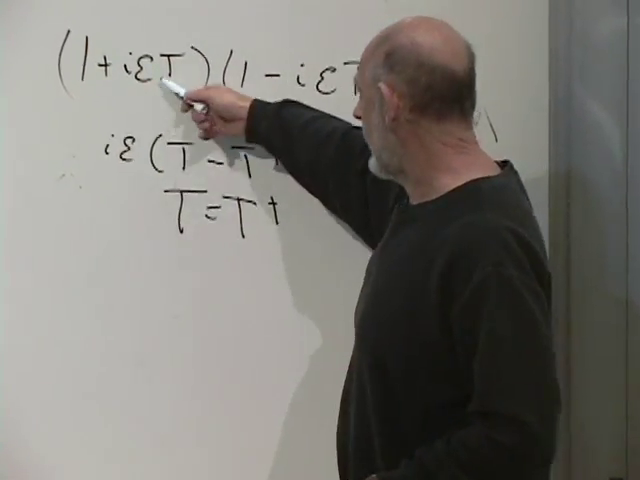
\includegraphics[width=0.62\textwidth]{lecture_04_figure_03.png}\caption{항등원에 가까운 유니터리 조건을 계산하면 \(T=T^\dagger\)이 됩니다.}\lectureframe{00:23:28}\end{figure}

공간 회전에는 독립적인 무한소 회전축이 세 개이므로 선형 독립인 생성자가 세 개 있습니다. 임의의 방향을 축으로 하는 작은 회전은 \(x\), \(y\), \(z\) 축을 중심으로 한 작은 회전들을 조합해 이룹니다. 이에 대응하는 생성자는 각운동량 연산자 \(J_x,J_y,J_z\)입니다. 이들의 교환자는 회전의 비가환성을 나타냅니다.
\begin{equation}
[J_i,J_j]=i\epsilon_{ijk}J_k.
\label{eq:l4-angular-momentum-algebra}
\end{equation}
무한소 회전을 반복하면 유한 회전이 만들어집니다.

유니터리성은 사용했지만 행렬식이 1이라는 조건은 아직 사용하지 않았습니다. 임의의 작은 행렬 \(m\)에 대해
\begin{equation}
\det(\boldsymbol 1+\epsilon m)
=1+\epsilon\,\operatorname{tr}m+O(\epsilon^2).
\label{eq:l4-det-expansion}
\end{equation}

\begin{figure}[htbp]\centering
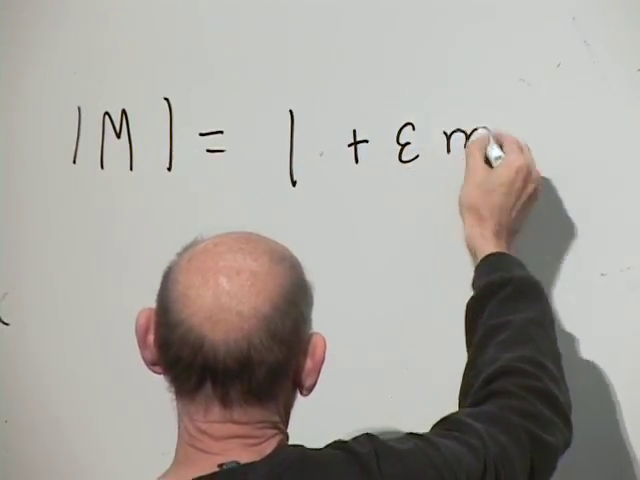
\includegraphics[width=0.62\textwidth]{lecture_04_figure_02.png}\caption{칠판에 적힌 행렬식의 1차 전개.}\lectureframe{00:21:51}\end{figure}

~\eqref{eq:l4-det-expansion}을 ~\eqref{eq:l4-infinitesimal-u}에 적용하면,
\begin{equation}
\det U
=1+i\epsilon\,\operatorname{tr}T+O(\epsilon^2).
\end{equation}
따라서 특수 유니터리 조건은 다음을 요구한다.
\begin{equation}
\operatorname{tr}T=0.
\label{eq:l4-traceless-generator}
\end{equation}
\(SU(2)\)의 생성자는 정확히 자취가 없는 에르미트 \(2\times2\) 행렬이다. 이 벡터 공간은 3차원이다. 파울리 행렬이 표준 기저를 이룬다.
\begin{equation}
\begin{aligned}
\sigma_x&=
\begin{pmatrix}0&1\\1&0\end{pmatrix},
&
\sigma_y&=
\begin{pmatrix}0&-i\\i&0\end{pmatrix},
\\[0.4em]
\sigma_z&=
\begin{pmatrix}1&0\\0&-1\end{pmatrix}.
\end{aligned}
\end{equation}
스핀 1/2 표현에서는 \(J_i=\sigma_i/2\)로 둘 수 있으므로, \(\hat{\boldsymbol n}\)을 축으로 \(\theta\)만큼 회전하는 유한 회전은
\begin{equation}
U(\hat{\boldsymbol n},\theta)
=\exp\!\left(-i\theta\,
\hat{\boldsymbol n}\cdot\boldsymbol\sigma/2\right).
\end{equation}
\editorialnote{유한 지수식은 무한소 생성자에 관한 논의를 표준적으로 마무리한다. 원문은 이 식을 명시적으로 쓰기보다 작은 회전을 반복하는 방식을 강조한다.}

\begin{classroomqa}
\audiencequestion{서로 독립인 자취 없는 에르미트 \(2\times2\) 행렬이 세 개라는 뜻인가요?
\lecturetimestamp{00:24:07}}
\lecturerresponse{그렇습니다. 파울리 행렬 세 개입니다. \(3\times3\) 특수 유니터리 행렬의 경우 이에 대응하는 개수는 여덟이며, 표준 기저는 겔만 행렬 여덟 개로 주어집니다.}
\end{classroomqa}

\begin{classroomqa}
\audiencequestion{그 여덟은 팔중도와 글루온 여덟 개에서 말하는 ``여덟''과 같은 건가요?
\lecturetimestamp{00:24:43}}
\lecturerresponse{수학적으로는 같은 유형의 \(SU(3)\) 표현론이지만, 어떤 \(SU(3)\) 대칭이 작용하는지 분명히 해야 합니다. 역사적인 팔중도 맛깔 대칭은 색 \(SU(3)\)이 아닙니다. 글루온 여덟 개는 색 \(SU(3)\)의 수반 표현에 속합니다.}
\end{classroomqa}

\section{SU(2)에서 색 SU(3)로}

이제 행렬을 \(2\times2\)에서 \(3\times3\)로 키워 봅시다. 일반적인 복소 \(3\times3\) 행렬에는 복소 성분이 아홉 개, 즉 실수 매개변수가 열여덟 개 있습니다. 조건 \(U^\dagger U=\boldsymbol 1\)은 실수 제약 아홉 개를 부과하고, \(\det U=1\)은 하나를 더 줄입니다. 따라서
\begin{equation}
18-9-1=8.
\end{equation}
독립적인 무한소 방향은 여덟 개이고 자취 없는 에르미트 생성자도 여덟 개입니다. \(SU(2)\)와 달리 이 군은 보통의 3차원 공간에서 회전군이 아닙니다. 색에 작용하는 내부 대칭입니다.

이 표현들을 쿼크에 적용하기 전에 합성 표현이 어떻게 생기는지 떠올려 봅시다. 스핀 1/2인 두 계를 포개고 궤도 운동은 무시합시다. 곱 상태는 네 개지만, 회전은 이 네 상태 전체를 기약적으로 섞지는 않습니다. 세 조합은 스핀 1처럼 변환합니다.
\begin{align}
\ket{1,1}&=\ket{\uparrow\uparrow},\\
\ket{1,0}&=\frac{1}{\sqrt2}
(\ket{\uparrow\downarrow}+\ket{\downarrow\uparrow}),\\
\ket{1,-1}&=\ket{\downarrow\downarrow},
\end{align}
네 번째 조합은 스핀 0처럼 변환합니다.
\begin{equation}
\ket{0,0}=\frac{1}{\sqrt2}
(\ket{\uparrow\downarrow}-\ket{\downarrow\uparrow}).
\end{equation}
따라서
\begin{equation}
\boldsymbol 2\otimes\boldsymbol 2
=\boldsymbol 3\oplus\boldsymbol 1.
\label{eq:l4-two-spin-decomposition}
\end{equation}
정렬된 상태가 삼중항의 \(m=\pm1\) 성분을 이루고, 대칭인 영 투영 상태가 삼중항을 완성하며, 반대칭 조합은 단일항입니다. 이것이 각운동량을 더하는 일반적인 원리이자 색 표현을 결합하는 원리입니다.

같은 단일항--삼중항 구분은 스핀 1/2 자유도 두 개를 결합할 때마다 나타납니다. 원자 수소에서는 전자와 양성자의 스핀이 초미세 단일항 및 삼중항 상태를 이룹니다. 오르토 수소와 파라 수소에서도 \(H_2\) 분자 안에 있는 두 양성자의 핵스핀에 같은 표현론이 적용됩니다.
\editorialnote{원문은 원자 수소의 양성자--전자 스핀을 언급하면서 ``오르토 및 파라 수소''라는 표현을 사용합니다. 수학적 분해는 맞습니다. 여기서는 정확성을 위해 분자 상태와 원자 상태의 명칭을 구분했습니다.}

\subsection{삼중항과 반삼중항}

쿼크 하나에는 세 가지 색 진폭이 있습니다. 선택한 기저에서 다음과 같이 씁니다.
\begin{equation}
q=
\begin{pmatrix}
q_r\\q_g\\q_b
\end{pmatrix},
\qquad
q'=Uq,
\qquad U\in SU(3).
\label{eq:l4-quark-triplet}
\end{equation}
세 성분은 쿼크 하나의 상태 진폭일 수도 있고, 빨강·초록·파랑 쿼크를 생성하는 세 장 연산자일 수도 있습니다. 군은 세 성분을 서로 섞습니다. 처음에 빨강인 상태는 일반적으로 색 변환 후 빨강·초록·파랑의 중첩 상태가 됩니다. 이 기본 3차원 표현을 \(\boldsymbol 3\)이라고 합니다.

반쿼크에는 쿼크 표현의 복소켤레를 통해 군이 작용합니다. 식~\eqref{eq:l4-quark-triplet}의 복소켤레를 취하면
\begin{equation}
\bar q'=U^*\bar q.
\end{equation}
이 표현을 \(\bar{\boldsymbol 3}\)라고 표기합니다. \(U(1)\)의 유비는 명확합니다. 전자장이 \(e^{i\theta}\)를 얻으면 양전자장은 \(e^{-i\theta}\)를 얻습니다. 쿼크와 반쿼크의 색 변환은 이 켤레 짝짓기의 비가환 버전입니다.

항등원 가까이에서 다음과 같다면
\begin{equation}
U=\boldsymbol 1+i\epsilon T,
\end{equation}
다음이 성립합니다.
\begin{equation}
U^*=\boldsymbol 1-i\epsilon T^*.
\end{equation}
따라서 반삼중항 생성자는 \(-T^*\), 즉 부호가 반대인 켤레입니다. 이것이 반쿼크가 반대 색전하를 가진다는 말의 정확한 의미입니다.

\begin{classroomqa}
\audiencequestion{\(SU(2)\)의 경우 복소켤레 표현은 어떻게 되나요?
\lecturetimestamp{00:36:19}}
\lecturerresponse{\(SU(2)\)의 이중항은 특별한 경우입니다. 반대칭 엡실론 텐서를 포함하는 고정된 기저 변환을 거치면 복소켤레 표현이 원래의 이중항과 동등합니다. \(SU(3)\)에서는 \(\boldsymbol 3\)와 \(\bar{\boldsymbol 3}\)가 실제로 서로 동등하지 않은 표현입니다.}
\end{classroomqa}
\editorialnote{\(SU(2)\) 기본 표현의 수학적으로 정확한 용어는 실수 표현이 아니라 유사실수 표현입니다. 답변은 원문의 의도된 구분을 유지하면서 용어를 바로잡았습니다.}

\section{색 표현의 결합}

기호 \(\otimes\)는 그 옆에 적힌 수를 보통의 방식으로 곱한다는 뜻이 아닙니다. 두 상태 공간을 결합한다는 뜻입니다. 그렇게 얻은 텐서곱 공간은 군 작용 아래 서로 섞이지 않는 부분들로 다시 분해됩니다.

\subsection{\texorpdfstring{\(\boldsymbol 3\otimes\boldsymbol 3\)}{두 쿼크: 33 x }}

쿼크 두 개에는 아홉 가지 색 기저 상태가 있습니다. 빨강--빨강, 빨강--초록, 빨강--파랑과 나머지 여섯 가지 순서쌍입니다. 두 색 지표를 대칭 부분과 반대칭 부분으로 나눠 봅시다. 대칭 부분에는 독립 성분이 여섯 개, 반대칭 부분에는 세 개 있습니다. \(SU(3)\)에서는
\begin{equation}
\boldsymbol 3\otimes\boldsymbol 3
=\boldsymbol 6\oplus\bar{\boldsymbol 3}.
\label{eq:l4-three-times-three}
\end{equation}

\begin{figure}[htbp]\centering
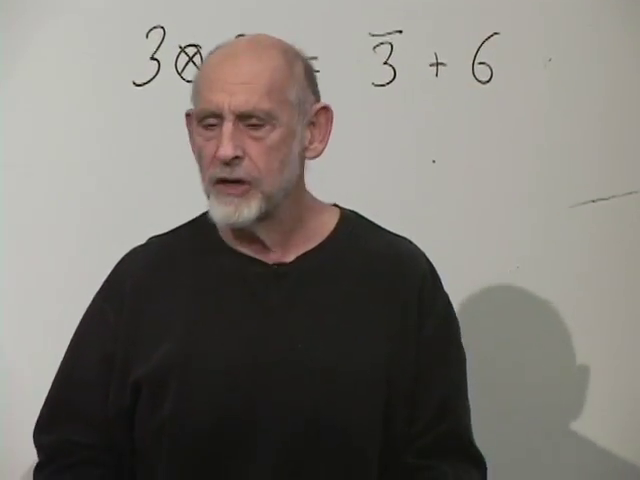
\includegraphics[width=0.68\textwidth]{lecture_04_figure_04.png}\caption{쿼크 두 개의 곱이 반삼중항과 육중항으로 분해됩니다.}\lectureframe{00:39:33}\end{figure}

반삼중항은 두 쿼크 지표를 불변 엡실론 텐서와 수축해 명시적으로 나타낼 수 있습니다.
\begin{equation}
(qq)^k_{\bar 3}
=\frac{1}{\sqrt2}\epsilon^{kij}q_iq_j.
\end{equation}
이 대상은 성분 세 개를 가지며 반쿼크처럼 변환합니다. 대칭 조합 여섯 개는 육중항을 이룹니다. 쿼크 두 개가 동역학적으로 반쿼크가 된다는 뜻이 아닙니다. 색 파동함수의 한 부분이 반쿼크와 같은 변환 법칙을 따른다는 뜻입니다.

\subsection{\texorpdfstring{\(\boldsymbol 3\otimes\bar{\boldsymbol 3}\)}{쿼크와 반쿼크: 3 x 반-3}}

쿼크--반쿼크 색 상태는 \(3\times3\) 행렬 \(M_i{}^j=q_i\bar q^j\)로 볼 수 있습니다. 모든 행렬은 자취 부분과 자취 없는 부분으로 유일하게 분해됩니다.
\begin{equation}
M=\frac{\operatorname{tr}M}{3}\boldsymbol 1
+\left(M-\frac{\operatorname{tr}M}{3}\boldsymbol 1\right).
\end{equation}
자취 부분은 불변 성분 하나이고, 자취 없는 부분에는 성분 여덟 개가 있습니다. 따라서
\begin{equation}
\boldsymbol 3\otimes\bar{\boldsymbol 3}
=\boldsymbol 1\oplus\boldsymbol 8.
\label{eq:l4-three-times-threebar}
\end{equation}
정규화 상수를 제외하면 단일항은 다음과 같습니다.
\begin{equation}
\ket{1}_{q\bar q}
=\frac{1}{\sqrt3}
(\ket{r\bar r}+\ket{g\bar g}+\ket{b\bar b}).
\end{equation}
불변이므로 다른 상태로 회전해 갈 수 없습니다. 나머지 여덟 선형 조합은 서로 섞입니다. 이들은 생성자 여덟 개가 변환하는 것과 같은 표현인 수반 표현을 이룹니다.

\subsection{세 쿼크}

세 번째 쿼크를 ~\eqref{eq:l4-three-times-three}와 결합하면 반삼중항 분기에서 다음을 얻는다.
\begin{equation}
\bar{\boldsymbol 3}\otimes\boldsymbol 3
=\boldsymbol 1\oplus\boldsymbol 8,
\end{equation}
따라서 세 쿼크의 곱에는 단일항이 포함된다. 전체 분해는 다음과 같다.
\begin{equation}
\boldsymbol 3\otimes\boldsymbol 3\otimes\boldsymbol 3
=\boldsymbol 1\oplus\boldsymbol 8\oplus\boldsymbol 8
\oplus\boldsymbol{10}.
\label{eq:l4-three-quark-full}
\end{equation}
색 단일항은 완전히 반대칭인 빨강--초록--파랑 조합이다.
\begin{equation}
\ket{1}_{qqq}
=\frac{1}{\sqrt6}\epsilon^{ijk}\ket{q_iq_jq_k}.
\label{eq:l4-baryon-singlet}
\end{equation}
\(\epsilon^{ijk}\)는 두 지수가 같을 때마다 0이므로, 0이 아닌 모든 항에는 빨강, 초록, 파랑 쿼크가 하나씩 들어가며, 두 지수를 서로 바꾸면 부호가 바뀐다.

\begin{classroomqa}
\audiencequestion{단일항이 아닌 조합은 단지 일어날 확률이 낮아서 확률을 무시해도 되나요?
\lecturetimestamp{00:46:02}}
\lecturerresponse{아닙니다. 문제는 확률이 아니라 에너지입니다. 고립된 비단일항은 색장을 무한히 먼 거리까지 끌고 가며, 가둠 영역에서는 무한한 에너지가 필요합니다. 이 주장의 배경이 되는 동역학은 아래에서 다루겠습니다.}
\end{classroomqa}

\subsection{글루온 팔중항}

글루온 장은 식~\eqref{eq:l4-three-times-threebar}의 팔중항처럼 변환합니다. 색과 관련해서는 삼중항 지표 하나와 반삼중항 지표 하나를 가지며, 단일항 자취 성분은 제거되어 있습니다. 개략적으로 쓰면
\begin{equation}
q\sim\boldsymbol 3,
\qquad
\bar q\sim\bar{\boldsymbol 3},
\qquad
G\sim\boldsymbol 8.
\end{equation}
이 기호들은 변환 법칙을 나타냅니다. 입자가 문자 그대로 정수 3이나 8과 같다는 뜻은 아닙니다.

아홉 번째 쿼크--반쿼크 색 조합은 항등행렬에 비례하며 단일항이므로 팔중항과 섞이지 않습니다. 그러므로 이를 제외해도 수학적으로 모순이 없습니다. \(SU(3)\) 게이지 장은 자취가 없고 성분이 여덟 개이며, \(U(3)\) 게이지 장의 아홉 성분과 다릅니다.

\begin{classroomqa}
\audiencequestion{자연은 왜 추가적인 단일항 글루온을 제외하나요?
\lecturetimestamp{00:49:00}}
\lecturerresponse{군론으로 바로 답하자면 단일항은 별개의 불변 부분 공간이므로 팔중항은 이를 포함하지 않아도 일관되게 닫혀 있습니다. \(SU(3)\)을 \(U(3)\) 대신 선택하는 더 깊은 이유는 여기서 유도하지 않습니다. 이는 양자색역학 현상론으로부터 추론한 게이지 구조의 일부입니다.}
\end{classroomqa}

\section{강입자로서의 색 단일항}

강한 상호작용에서 자유롭게 존재하는 유한 질량 입자는 색 단일항입니다. 그렇다고 쿼크나 글루온이 실재하지 않는다는 뜻은 아닙니다. 이들이 고립된 점근 입자로 나타나지 않는다는 뜻입니다. 단일항을 만드는 기본 형태는 다음과 같습니다.
\begin{equation}
qqq,
\qquad
q\bar q,
\qquad
GG\ \text{and higher gluonic products}.
\end{equation}
각각 중입자, 중간자, 글루볼로 이어집니다. 이미 색을 띠지 않는 대상 여러 개를 곱해도 여전히 색을 띠지 않으므로, 더 복잡한 다중 강입자 상태도 이 구성 요소들로 만들 수 있습니다.

\begin{classroomqa}
\audiencequestion{쿼크 세 개와 쿼크--반쿼크의 단일항은 각각 무엇이라 부르며, 글루온도 단일항을 만들 수 있나요?
\lecturetimestamp{00:51:38}}
\lecturerresponse{쿼크 세 개의 단일항은 중입자이고, 쿼크--반쿼크 단일항은 중간자입니다. 글루온도 결합해 색 단일항을 이룰 수 있습니다. 가장 단순한 강한 상호작용 상태를 글루볼이라 하며, 글루온 두 개보다 많이 참여할 수도 있습니다.}
\end{classroomqa}

스핀 1/2 쿼크 세 개는 항상 전체 스핀이 반정수가 되도록 결합하지만, 궤도 각운동량에 따라 어떤 반정수가 되는지는 달라질 수 있습니다. 쿼크--반쿼크 중간자의 스핀은 정수입니다. 순수하게 글루온으로 이루어진 글루볼도 스핀이 정수입니다.

글루온 두 개에 대한 칠판의 첫 설명은 단지 개수를 셉니다.
\begin{equation}
8\times8=1+63.
\end{equation}
색 상태는 모두 64개입니다. 그중 한 조합은 단일항이고 나머지 63개는 단일항이 아닌 부분 공간에 속합니다.

\begin{figure}[htbp]\centering
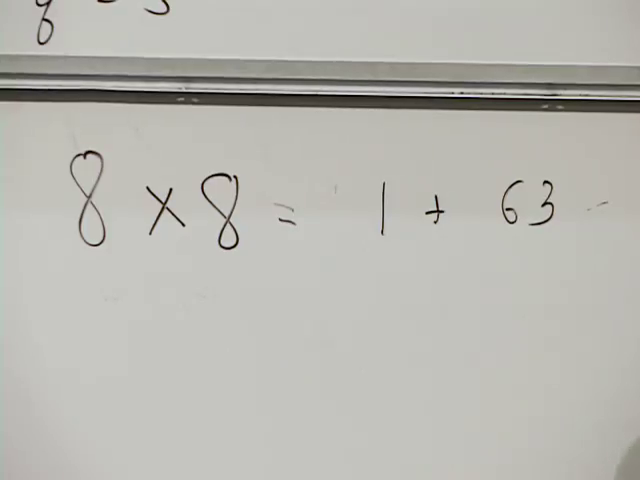
\includegraphics[width=0.68\textwidth]{lecture_04_figure_05.png}\caption{두 글루온 상태의 개수: 64개 상태 가운데 단일항 하나.}\lectureframe{00:53:44}\end{figure}

기약 표현으로 완전히 분해하면 다음과 같습니다.
\begin{equation}
\boldsymbol 8\otimes\boldsymbol 8
=\boldsymbol 1\oplus\boldsymbol 8_S\oplus\boldsymbol 8_A
\oplus\boldsymbol{10}\oplus\overline{\boldsymbol{10}}
\oplus\boldsymbol{27}.
\label{eq:l4-eight-times-eight}
\end{equation}
차원의 합은 다음과 같이 맞습니다.
\begin{equation}
1+8+8+10+10+27=64.
\end{equation}
두 팔중항은 서로 다른 불변 부분 공간입니다. 하나는 수반 표현 인자 두 개의 교환에 대해 대칭이고, 다른 하나는 반대칭입니다. 단일항은 글루볼 상태를 만들 수 있는 두 글루온 색 채널입니다.
\editorialnote{칠판에서는 먼저 \(8\times8=1+63\)만 제시됩니다. 뒤이은 수업 중 문답에서 열거된 기약 차원이 나옵니다. 막대와 대칭성 표기는 표준 \(SU(3)\) 표기법에 맞춰 복원했습니다.}

\subsection{관측되는 전하가 정수인 이유}

쿼크 전하에는 두 종류가 있습니다.
\begin{equation}
Q_{\mathrm{up\text{-}like}}=+\frac23,
\qquad
Q_{\mathrm{down\text{-}like}}=-\frac13.
\end{equation}
따라서 쿼크 세 개의 총전하는 정수입니다. 업형 쿼크가 몇 개인지에 따라 \(-1,0,+1,\text{ or }+2\)가 됩니다. 쿼크와 반쿼크의 전하도 마찬가지로 \(0\) 또는 \(\pm1\)입니다. 글루온은 전기 전하를 띠지 않습니다. 따라서 관측된 쿼크 표현으로 만든 기본 색 단일항은 구성 입자의 전하가 분수여도 전기 전하가 정수입니다.

\begin{classroomqa}
\audiencequestion{기묘 쿼크의 전기 전하는 얼마인가요?
\lecturetimestamp{00:56:08}}
\lecturerresponse{다운형 쿼크이므로 전하는 \(-1/3\)입니다. 세 세대에서도 같은 전하 패턴이 반복됩니다. \((u,d)\), \((c,s)\), \((t,b)\)이며, 각 쌍의 전하는 \(+2/3\)와 \(-1/3\)입니다.}
\end{classroomqa}

이 입자 구성에서는 색 단일항 조건과 전기 전하의 정수성이 밀접하게 연결되어 있지만, 수학적으로 같은 명제는 아닙니다. 전하가 정수라는 결론에는 방금 제시한 특정 표준모형 전하 배정도 필요합니다.

\begin{classroomqa}
\audiencequestion{색 단일항은 얽힌 상태인가요? 그렇다면 벨 실험의 얽힌 쌍과 같은 의미가 있나요?
\lecturetimestamp{00:56:58}}
\lecturerresponse{단일항 색 파동함수는 분명 얽혀 있습니다. 각 색이 따로 확정된 곱상태가 아니라 결맞은 중첩 상태입니다. 원칙적으로 구성 입자들을 서로 떼어 놓을 수는 있지만, 가둠 때문에 분리에 드는 비용은 점점 커지고 결국 새로운 강입자가 만들어집니다. 그러므로 상태는 얽혀 있지만 벨 실험 방식으로 조작하기에는 적합한 계가 아닙니다.}
\end{classroomqa}

\section{텐서곱 방정식의 의미}

이제 곱셈표를 좀 더 구체적으로 설명할 필요가 있습니다. \(\psi_i\)와 \(\phi_j\)를 스핀 1/2인 두 대상을 생성하는 연산자라고 합시다. 전자와 양성자처럼 서로 다른 종을 나타낼 수도 있고, 적절한 통계성을 고려한 같은 종의 두 복사본을 나타낼 수도 있습니다. 각 지표는 두 값을 취합니다. 네 가지 곱
\begin{equation}
\psi_\uparrow\phi_\uparrow,
\quad
\psi_\uparrow\phi_\downarrow,
\quad
\psi_\downarrow\phi_\uparrow,
\quad
\psi_\downarrow\phi_\downarrow
\end{equation}
이 텐서곱 공간을 생성합니다.

군 원소가 각 인자에 \(U\)로 작용한다면, 곱에 대해서는 \(U\otimes U\)로 작용합니다. 성분으로 쓰면
\begin{equation}
\psi_i\phi_j
\longmapsto
U_i{}^kU_j{}^\ell\psi_k\phi_\ell.
\label{eq:l4-product-action}
\end{equation}
이 표현은 4차원이지만 가약 표현입니다. 반대칭 조합
\begin{equation}
\frac{1}{\sqrt2}
(\psi_\uparrow\phi_\downarrow
-\psi_\downarrow\phi_\uparrow)
\end{equation}
은 자기 자신으로 사상되는 반면, 대칭인 세 조합은 서로 사이에서 사상됩니다. 이 조합에 맞는 기저에서는 모든 곱 표현 행렬이 다음과 같은 블록 대각 형태를 띱니다.
\begin{equation}
D_{2\otimes2}(g)
\sim
\begin{pmatrix}
1&0\\
0&D_3(g)
\end{pmatrix}.
\label{eq:l4-spin-block-diagonal}
\end{equation}

\begin{classroomqa}
\audiencequestion{\(\boldsymbol 3\otimes\boldsymbol 3=\bar{\boldsymbol 3}\oplus\boldsymbol 6\)와 같은 방정식은 어떤 연산을 나타내나요?
\lecturetimestamp{00:57:51}}
\lecturerresponse{좌변은 합성 상태 공간을 이룹니다. 군은 두 인자 모두에 작용하므로 곱 기저 상태들을 섞습니다. 우변은 기저를 바꾸면 상태들이 불변 집합으로 나뉜다는 뜻입니다. 세 반대칭 조합은 반삼중항처럼 변환하고, 여섯 대칭 조합은 육중항처럼 변환합니다. 더하기 기호는 보통의 수치 덧셈이 아니라 직합을 뜻합니다.}
\end{classroomqa}

\begin{classroomqa}
\audiencequestion{아홉 상태가 \(3+6\), 또는 \(1+8\)로 분해된다는 것은 어떻게 알 수 있나요? 예를 들어 \(2+7\)일 수도 있지 않나요?
\lecturetimestamp{01:04:39}}
\lecturerresponse{차원만 세어서는 분해를 결정할 수 없습니다. \(SU(3)\)이 어떤 기약 표현을 갖는지 알아야 하고, 지표를 대칭화하거나 반대칭화하거나 자취 부분과 자취 없는 부분을 분리하는 등 불변 부분 공간을 구성해야 합니다. 완전한 분류에는 더 많은 군론이 필요합니다. 여기서는 쿼크와 글루온에 필요한 표현만 사용합니다.}
\end{classroomqa}

불변 엡실론 텐서를 쓰면 단일항 구성이 명확해집니다. \(SU(2)\)에 대해
\begin{equation}
\epsilon_{ij}U^i{}_kU^j{}_\ell
=(\det U)\epsilon_{k\ell}
=\epsilon_{k\ell}.
\end{equation}
따라서 \(\epsilon_{ij}\psi^i\phi^j\)는 불변입니다. \(SU(3)\)에서는 세 지표를 가진 버전으로 다음을 얻습니다.
\begin{equation}
\epsilon_{ijk}U^i{}_aU^j{}_bU^k{}_c
=(\det U)\epsilon_{abc}
=\epsilon_{abc},
\end{equation}
이는 식~\eqref{eq:l4-baryon-singlet}의 쿼크 세 개 상태가 불변임을 증명합니다.

\begin{classroomqa}
\audiencequestion{단일항이 변환되지 않는 이유를 명시적으로 보일 수 있나요?
\lecturetimestamp{01:07:18}}
\lecturerresponse{네. 모든 기본 지표를 완전 반대칭 엡실론 텐서와 수축하면 됩니다. 변환 아래에서는 행렬들의 곱이 엡실론에 \(\det U\)를 곱합니다. 특수 유니터리 행렬의 행렬식은 1이므로 수축한 상태는 변하지 않습니다. \(SU(2)\)에서는 이것이 두 스핀 단일항을 증명하고, \(SU(3)\)에서는 빨강--초록--파랑 쿼크 세 개의 단일항을 증명합니다.}
\end{classroomqa}

\begin{classroomqa}
\audiencequestion{글루온 팔중항 두 개의 완전한 분해는 무엇인가요?
\lecturetimestamp{01:09:24}}
\lecturerresponse{식~\eqref{eq:l4-eight-times-eight}에 나온 분해입니다. 단일항 하나, 팔중항 두 개, 십중항 하나, 반십중항 하나, 그리고 27차원 표현 하나입니다. 팔중항 지표 두 개로 만들 수 있는 색 단일항 조합은 정확히 하나입니다.}
\end{classroomqa}

\begin{classroomqa}
\audiencequestion{쿼크 세 개의 완전한 분해는 이에 대응해 어떻게 되나요?
\lecturetimestamp{01:11:51}}
\lecturerresponse{물리적으로 핵심적인 답은 단일항이 하나 포함된다는 것입니다. 차원 계산까지 완성하면 식~\eqref{eq:l4-three-quark-full}을 얻습니다. 단일항 하나, 팔중항 두 개, 십중항 하나이며 전체 상태 수는 \(1+8+8+10=27\)입니다.\editorialnote{문답 중 강의자는 완전한 \(3\otimes3\otimes3\) 분해를 기억하지 못합니다. 여기에는 표준적인 완성 결과를 명시적으로 보충하고, 이를 구두 답변에 귀속시키지 않았습니다.}}
\end{classroomqa}

같은 생각을 두 글루온 공간으로 확장할 수 있다. 순진한 곱 기저에서는
\(SU(3)\)가 \(64\times64\) 행렬로 작용한다. 기약 성분에 맞춘 기저에서는 이 행렬들이 블록 대각 형태가 된다.
\begin{equation}
\begin{aligned}
D_{8\otimes8}(g)
&\sim
\operatorname{diag}\bigl(
1,D_{8_S}(g),D_{8_A}(g),
\\
&\hspace{4.8em}
D_{10}(g),D_{\overline{10}}(g),D_{27}(g)
\bigr).
\end{aligned}
\end{equation}
어느 블록도 다른 블록과 섞이지 않지만, 각 블록 안의 상태들은 서로 섞인다.

\begin{classroomqa}
\audiencequestion{텐서곱 분해란 큰 표현 행렬이 블록 대각 형태가 되는 기저로 바꾸는 것뿐인가요?
\lecturetimestamp{01:12:02}}
\lecturerresponse{맞습니다. 두 스핀의 경우 4차원 행렬이 1차원 단일항 블록과 3차원 삼중항 블록으로 바뀝니다. 두 글루온의 경우 64차원 행렬이 차원이 \(1,8,8,10,10,\text{ and }27\)인 블록들로 바뀝니다. 각 블록은 모든 군 변환 아래에서 닫혀 있습니다.}
\end{classroomqa}

\begin{classroomqa}
\audiencequestion{전체 텐서곱 공간 안의 그런 닫힌 부분을 부르는 이름이 있나요?
\lecturetimestamp{01:14:55}}
\lecturerresponse{그것은 부분표현을 이루는 불변 부분공간입니다. 더 이상 분해할 수 없으면 기약 표현, 즉 irrep을 이룹니다. 전체 텐서곱은 그런 기약 성분들의 직합입니다.\editorialnote{강의 중에는 질문에서 요청한 용어가 나오지 않는다. 답변에서는 표준 표현론 용어를 제시한다.}}
\end{classroomqa}

\begin{classroomqa}
\audiencequestion{비단일항인 십중항과 다른 표현들을 존재하지 않는다고 부를 때, 완전히 무시해야 한다는 뜻인가요?
\lecturetimestamp{01:15:36}}
\lecturerresponse{그 표현들은 타당한 색 섹터이며 중간 계산에서 중요하지만, 실험실에서 고립된 유한 에너지 입자로 나타나지는 않습니다. 자유 점근 상태가 되지 못하게 하는 것은 표현론의 실패가 아니라 색 가둠입니다.}
\end{classroomqa}

\section{남부의 색 개념에서 색 가둠까지}

색 개념은 QCD의 최종 정식화보다 앞서 나왔다. 요이치로 남부는 이미 1960년대 초에 숨겨진 세 가지 값의 양자수가 눈에 띄는 문제를 해결할 수 있음을 이해했다. 쿼크는 분수 전하를 띠지만, 분수 전하를 가진 자유 입자는 관측되지 않는다는 문제였다. 물리적 상태가 색 단일항으로 제한되면 쿼크는 앞서 설명한 정수 전하 조합으로 나타난다. 남은 문제는 동역학적이다. 유한 에너지 자유 상태가 모두 단일항이 되도록 하는 힘은 무엇인가?

전자기학의 비유부터 살펴보자. 전하와 반대 부호의 전하는 서로 끌어당긴다. 둘을 가까이 가져가면 에너지가 낮아지고, 같은 부호의 전하를 가까이 밀어 붙이려면 일이 필요하다. 장 자체에는 양의 에너지가 저장된다.
\begin{equation}
E_{\mathrm{field}}
=\frac12\int d^3x\,\boldsymbol E^2
\end{equation}
단순한 정전기 단위계에서 성립하는 식이다. 순전하가 있으면 장이 계 바깥 먼 곳까지 뻗어나가지만, 단단히 결합한 중성 쌍에는 근거리 쌍극자 장만 남는다. 따라서 중성화하면 바깥쪽 장 에너지가 사라진다.

전자기 결합을 엄청나게 키운다고 상상해 보자. 순전하에 따른 장 에너지 페널티가 매우 커져 낮은 에너지의 물체는 압도적으로 중성이 되고, 하전된 구성 성분을 떼어내는 비용은 감당하기 어려울 만큼 커질 수 있다. 남부는 이 직관을 색에 적용했다. 여덟 색 전하는 여덟 글루온 장의 원천이므로, 큰 색 장 에너지가 고립된 비단일항 상태를 금지할 수 있다는 생각이었다.

이 직관은 대체로 옳지만, QCD에는 결정적인 새로운 특징이 있다. 광자는 전하를 띠지 않지만 글루온은 색을 띤다. 광자는 고전 전자기장의 원천이 아니며, 맥스웰 방정식은 선형이므로 전자기파 두 개는 중첩되어 서로 통과한다. 글루온은 색 팔중항으로 변환되므로 글루온은 다른 글루온의 원천이 되고 서로 상호작용한다. 하나의 글루온 장 안에서 서로 다른 부분들도 상호작용한다. 따라서 비가환 게이지 장은 비선형이다.

\subsection{플럭스 튜브와 선형 퍼텐셜}

장거리에서 글루온의 자기상호작용은 색 플럭스가 보통의 전기 쌍극자 장처럼 퍼져 나가는 것을 막는다. 플럭스는 쿼크와 반쿼크를 잇는 튜브 안으로 압축된다. 긴 튜브의 장 세기와 단면적은 대략 일정하므로, 튜브에는 길이당 에너지가 대략 일정하게 저장된다. \(\sigma\)를 이 끈 장력이라고 하면,
\begin{equation}
V(R)\simeq\sigma R+\text{constant}
\qquad (R\ \text{large}).
\label{eq:l4-linear-potential}
\end{equation}

\begin{figure}[htbp]
\centering
\includegraphics[width=0.78\textwidth]{lecture_04_figure_06.png}
\caption{쿼크와 반쿼크 사이의 긴 튜브 안에 모인 색 플럭스.}
\lectureframe{01:31:35}
\end{figure}

이는 크기가 \(1/R\)처럼 감소하는 쿨롱 퍼텐셜보다 더 강한 효과다. 색 전하들을 더 멀리 떨어뜨려도 힘이 끝없이 약해지지 않는다. 튜브가 길어지면서 에너지가 계속 더해진다. 무한한 부피 안의 고립된 색 전하에는 끝없이 뻗는 튜브가 필요하므로 에너지가 무한히 커진다. 색 단일항만 유한 에너지 점근 상태를 이룬다는 말의 실제 의미가 바로 이것이다.
\editorialnote{끈 장력 표기와 장거리 퍼텐셜을 명시하여, 균일한 플럭스 튜브가 길이당 균일한 에너지를 가진다는 원문의 설명을 정량적으로 나타낸다.}

\subsection{끈 끊어짐과 제트}

메손 안의 쿼크 하나가 고에너지 충돌을 받는다고 하자. 쿼크가 멀어지기 시작하면 플럭스 튜브가 뒤에서 늘어난다. 쿼크는 운동 에너지를 잃고 다시 끌려올 수 있다. 더 흔하게는 저장된 장 에너지가 충분히 커지면 진공에서 새 쿼크--반쿼크 쌍이 생성된다. 새 반쿼크는 멀어지는 쿼크에 연결된 플럭스를 끝내고, 새 쿼크는 원래 반쿼크에 연결된 플럭스를 끝낸다. 늘어난 단일항 하나가 더 짧은 단일항 둘로 바뀐다.
\begin{equation}
(q\bar q)_{\mathrm{stretched}}
\longrightarrow
(q\bar q)+(q\bar q).
\label{eq:l4-string-breaking}
\end{equation}

\begin{figure}[htbp]
\centering
\includegraphics[width=0.78\textwidth]{lecture_04_figure_07.png}
\caption{쌍 생성은 늘어난 플럭스 튜브 하나를 색 단일항 튜브 두 개로 분리한다.}
\lectureframe{01:34:52}
\end{figure}

\begin{classroomqa}
\audiencequestion{충돌로 튕겨 나온 쿼크가 튜브를 계속 늘릴 만큼 충분한 에너지를 지녔다면, 다시 끌려오는 것 외에 어떤 일이 일어날 수 있나요?
\lecturetimestamp{01:33:50}}
\lecturerresponse{튜브는 쿼크--반쿼크 쌍 생성으로 끊어질 수 있습니다. 튜브의 에너지는 새 쌍의 질량과 운동 에너지가 됩니다. 양 끝이 다시 연결되어 단일항 둘을 이루므로, 이 과정은 고립된 쿼크가 아니라 추가 메손을 생성합니다.}
\end{classroomqa}

그 파톤들 가운데 하나가 여전히 큰 운동량을 지니면 과정이 반복된다. 그 결과 원래 파톤의 진행 방향 주위로 집중된 색 단일항 하드론의 연쇄가 만들어진다. 이를 제트라고 한다. 에너지가 큰 쿼크와 글루온이 하드론으로 바뀌는 과정을 하드론화라고 한다. 제트를 통해 처음 생성된 색 전하 입자를 추론할 수는 있지만, 그 입자 자체가 관측되는 것은 아니다.

\begin{classroomqa}
\audiencequestion{끈 끊어짐으로 메손만 만들어지나요, 아니면 제트에서 다른 하드론도 나올 수 있나요?
\lecturetimestamp{01:35:20}}
\lecturerresponse{물론 다른 하드론도 나올 수 있습니다. 최종적으로 관측되는 물체가 단일항이면 된다는 것이 색에 관한 유일한 조건입니다. 한 번 끊어지는 경우에는 메손이 가장 간단한 그림이지만, 바리온과 반바리온, 더 복잡한 단일항 조합도 생성될 수 있습니다.}
\end{classroomqa}

쿼크 세 개는 색 단일항 접합부에서 플럭스를 끝낼 수 있다. 세 갈래로 뻗는 이 그림은 식~\eqref{eq:l4-baryon-singlet}의 반대칭 엡실론 텐서에 대응하는 동역학적 그림이다. 완전한 바리온에서는 순 색 플럭스가 바깥으로 빠져나오지 않는다.

\begin{figure}[htbp]
\centering
\includegraphics[width=0.72\textwidth]{lecture_04_figure_08.png}
\caption{메손의 끈 끊어짐 그림 아래에 나타낸 바리온의 세 갈래 색 플럭스 접합부.}
\lectureframe{01:36:12}
\end{figure}

\section{게이지 장, 보존 전하와 표준모형}

현재 수준에서 게이지 이론은 보존 전하가 광자와 비슷한 장의 원천이 되는 이론으로 이해할 수 있다. 전하는 전자기장의 원천이고, 여덟 색 전하는 여덟 글루온 장의 원천이다. 더 깊은 정식화에서는 대칭을 국소화하고, 이웃한 시공간 점에서 내부 상태를 비교하는 접속을 도입한다. 그러나 여기서 다루는 색 가둠의 그림에는 그런 구성이 필요하지 않다.
\editorialnote{게이지 이론의 더 깊은 표준적 의미는 국소 대칭을 정식화하는 것으로, 원문에서도 언급만 하고 뒤로 미뤄 둔다.}

대칭, 보존 전하와 플럭스는 긴밀히 연결되어 있다. 장선이 전하에서만 끝날 수 있다면, 원천은 플럭스가 아무것에도 연결되지 않은 채 남도록 그냥 사라질 수 없다. 또한 장의 변화는 인과적으로 전파되므로 그 원천의 먼 곳에 있는 장이 모두 순간적으로 사라질 수도 없다. 국소적인 형태로 같은 물리는 연속 방정식으로 표현된다.
\begin{equation}
\frac{\partial\rho}{\partial t}
+\boldsymbol\nabla\cdot\boldsymbol j=0,
\end{equation}
이 식은 전하가 경계를 통과해 흐를 때만 한 영역 밖으로 나갈 수 있음을 뜻한다. 장선에 관한 논증은 이 국소 보존 법칙을 기하학적으로 그린 것이다.

이제 표준모형 안에서 이 결과가 어디에 놓이는지 살펴볼 수 있다. 색 섹터에는 \(SU(3)\)의 생성원 여덟 개와 이에 대응하는 글루온 장 여덟 개가 있다. 아벨 섹터에는 생성원 하나와 게이지 장 하나가 있다. 생성원 세 개는 보통의 공간 각운동량이 아니라 추가적인 \(SU(2)\)에 속한다. 대칭 깨짐 전 게이지 구조는 다음과 같다.
\begin{equation}
SU(3)_c\times SU(2)_L\times U(1)_Y,
\end{equation}
생성원은 모두 \(8+3+1=12\)개다. 다음으로 전약 \(SU(2)\)을 이해한 뒤, 힉스 장과 관측되는 광자, \(W^\pm\), \(Z\)가 어떻게 나타나는지 살펴보자.
\editorialnote{원문은 광자를 여덟 글루온과 함께 세고, 나머지 인자를 \(SU(2)\times U(1)\)라고 설명한다. 깨지지 않은 표준모형에서 아벨 인자는 초전하 \(U(1)_Y\)이다. 광자는 전약 혼합 뒤에야 나타난다.}

이제 핵심 논리의 연결이 완성되었다. 추상군은 표현을 통해 작용하고, 무한소 생성원은 보존 전하이며, 쿼크와 반쿼크, 글루온은 각각 \(\boldsymbol 3\), \(\bar{\boldsymbol 3}\), \(\boldsymbol 8\) 표현에 속한다. 텐서곱은 단일항 하드론을 식별하고, 비선형 글루온 장은 단일항 선택을 색 가둠이라는 물리적 현상으로 만든다.

\chapter{게이지 장, 상호작용 척도 및 하전 약전류}

양자전기역학과 양자색역학은 실험실에서 보면 매우 달라 보이지만, 둘 다 게이지 이론이다. 사실 표준모형의 거의 모든 상호작용은 이런 방식으로 구성된다. \emph{게이지}라는 말에는 국소 대칭과 관련된 더 깊은 의미가 있지만, 그 수학적 틀은 뒤로 미뤄도 된다. 지금은 최소한의 물리적 설명이면 충분하다. 게이지 이론에는 맥스웰 이론과 비슷한 장, 보존되는 원천, 대칭 변환, 게이지 보손, 그리고 그 보손을 방출하고 흡수하는 규칙이 들어 있다.

\section{원형이 되는 맥스웰 이론}

\subsection{장과 퍼텐셜}

전자기장은 성분이 여섯 개다. 전기장 성분이 셋, 자기장 성분이 셋이다. 이와 같은 정보를 중복성을 허용하는 사차원 벡터 퍼텐셜로 나타낼 수도 있다.
\begin{equation}
A_\mu=(A_0,\boldsymbol A),
\end{equation} 여기서 \(A_0\)는 정전기 퍼텐셜이고 \(\boldsymbol A\)는 공간 벡터 퍼텐셜이다. 정전기적 한계에서는 공간 기울기로부터 전기장을 구한다.
\begin{equation}
\boldsymbol E=-\boldsymbol\nabla A_0,
\qquad
\boldsymbol F=q\boldsymbol E,
\end{equation} 한편 자기장은 다음과 같다.
\begin{equation}
\boldsymbol B=\boldsymbol\nabla\times\boldsymbol A.
\end{equation} 첫 번째 식의 부호는 퍼텐셜의 표준적인 정의에 따라 달라진다. 칠판에서 다룬 핵심은 장이 퍼텐셜의 미분으로 주어진다는 점이다.
\editorialnote{시간에 따라 변하는 장의 완전한 관계식은 다음과 같다.
\(\boldsymbol E=-\boldsymbol\nabla A_0-\partial_t\boldsymbol A\) 여기서는 의도적으로 더 단순한 정전기적 수준에서 설명한다.}

\begin{figure}[htbp]\centering
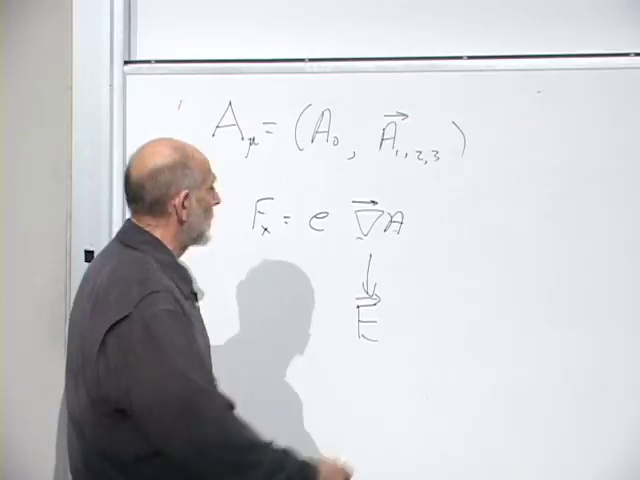
\includegraphics[width=0.62\textwidth]{lecture_05_figure_02.png}\caption{전자기 사차원 퍼텐셜과 장에 대한 미분 관계.}\lectureframe{00:03:33}\end{figure}

따라서 전기역학은 서로 동등한 두 가지 방식으로 기술할 수 있다. 하나는 \(\boldsymbol E\)와 \(\boldsymbol B\)를 사용하는 방식이고, 다른 하나는 \(A_\mu\)를 사용하는 방식이다. 후자에 표시된 성분은 네 개뿐인데, 서로 다른 퍼텐셜이 동일한 물리적 장을 나타낼 수 있기 때문이다. 이 중복성이 게이지라는 말의 배경을 처음으로 보여 주지만, 아직 형식적으로 사용하지는 않겠다.

\subsection{파동과 편광}

맥스웰 방정식은 파동을 허용한다. 단위 벡터 \(\hat{\boldsymbol k}\) 방향으로 진행하는 평면파를 생각해 보자. 모든 지점에서 전기장과 자기장은 횡방향이다.
\begin{equation}
\boldsymbol E\cdot\hat{\boldsymbol k}=0,
\qquad
\boldsymbol B\cdot\hat{\boldsymbol k}=0,
\qquad
\boldsymbol E\cdot\boldsymbol B=0.
\end{equation} \(c=1\)인 단위계에서는 두 장의 크기가 같다.
\begin{equation}
|\boldsymbol E|=|\boldsymbol B|.
\end{equation} 선편광파에서는 \(\boldsymbol E\)의 방향이 편광을 지정한다. 파동의 전체 무늬는 빛의 속도로 전파된다.

양자화는 서술 방식을 바꾸지만 편광 구조는 바꾸지 않는다. 전자기파의 양자는 광자다. 광자를 점으로 그리면 필연적으로 오해를 부르지만, 그 점이 편광을 나타내는 작은 횡방향 화살표를 지닌다고 상상하면 유용하다. 사분파장판이나 다른 광학 소자는 그 편광을 회전시킬 수 있다. 정적인 쿨롱 장도 아주 거칠게나마 광자의 반복적인 방출과 흡수에서 생긴다고 그려 볼 수 있다.

\subsection{원천, 플럭스 및 보존}

전자기파는 빈 공간에서도 전파되지만, 장에는 전하와 전류라는 원천도 있다. 양전하를 띤 점전하는 \(1/r^2\)에 비례하는 바깥쪽 방사형 전기장을 만든다. 전하를 둘러싼 구면을 통과하는 장선의 수는 구면의 반지름과 무관하다. 수식으로 쓰면 다음과 같다.
\begin{equation}
\oint_{S^2}\boldsymbol E\cdot d\boldsymbol S
=\frac{Q_{\mathrm{enc}}}{\epsilon_0},
\label{eq:l5-gauss}
\end{equation} SI 단위계에서의 식이다.

이는 장을 계산하는 편리한 방법에 그치지 않는다. 전기장선은 전하에서만 끝날 수 있다. 고립된 전하 하나가 그저 사라진다면, 인과율을 위반하면서 그 장이 모든 곳에서 동시에 사라져야 한다. 그렇지 않으면 장선이 빈 공간에서 끝나는, 장이 사라진 영역의 경계가 바깥으로 전파되어야 한다. 둘 다 허용되지 않는다. 따라서 선속의 기하학적 구조는 전하 보존을 자연스럽게 만든다. 전하는 움직일 수 있고 서로 반대인 전하는 소멸할 수 있지만, 보상하는 전류 없이 순전하가 국소적으로 사라질 수는 없다.

이에 대응하는 국소적 진술은 연속 방정식이다.
\begin{equation}
\partial_t\rho+\boldsymbol\nabla\cdot\boldsymbol J=0.
\label{eq:l5-continuity}
\end{equation}
\editorialnote{~\eqref{eq:l5-continuity} 방정식은 강의에서 말로 전개한 인과적 선속 논증을 표준적인 국소 수학 형식으로 나타낸 것이다.}

\subsection{게이지 이론의 실용적 정의}

이제 작동상의 전형을 서술할 수 있다. 게이지 이론에는 다음이 있다.
\begin{itemize}\item 전기장과 유사한 장 및 자기장과 유사한 장;
\item 상호작용이 충분히 약할 때 빛의 파동과 비슷한 파동;
\item 전하와 유사한 원천;
\item 선속과 그 원천을 연결하는 가우스 법칙;
\item 보존 법칙과 이에 대응하는 대칭;
\item 게이지 보손이라 부르는 장의 양자;
\item 방출과 흡수를 제어하는 결합 상수.
\end{itemize}
원천이 반드시 전하일 필요는 없다. 의도적으로 비현실적인 예로 바리온 수를 게이지 대칭으로 만든다고 상상해 보자. 양성자와 중성자는 모두 바리온 수 \(+1\)를 가지므로 새로운 쿨롱 유사 힘으로 서로 밀어내고, 양성자와 반양성자는 서로 끌어당길 것이다. 이런 이론은 수학적으로 상상할 수 있지만, 자연에는 바리온 수와 결합하는 장거리 게이지 장이 관측되지 않는다. 보존 법칙이 있다고 해서 게이지 힘까지 반드시 존재하는 것은 아니다.

전하에는 실제로 대칭이 따른다. 전하를 띤 물질장에 대해,
\begin{equation}
\psi(x)\longmapsto e^{i\theta}\psi(x).
\label{eq:l5-u1}
\end{equation}
위상 대칭과 전하 보존은 같은 구조의 양면이다. 나중에 \(\theta\)를 시공간에 따라 달라지게 해 보면 퍼텐셜 \(A_\mu\)가 왜 필요한지 알 수 있다. 여기서는 전역 변환만으로도 보존 전하를 확인하기에 충분하다.

\section{비아벨 예로서의 양자색역학}

\subsection{삼중항, 반삼중항 및 글루온 행렬}

양자색역학에서 쿼크장은 색 지표 \(i\in\{r,g,b\}\)를 가지며 \(SU(3)\)의 기본 표현으로 변환한다.
\begin{equation}
q'_i=U_{ij}q_j,
\qquad
U^\dagger U=\boldsymbol 1,
\qquad
\det U=1.
\label{eq:l5-q-transform}
\end{equation} 이는 삼차원 복소 색 공간에서의 회전이지, 통상적인 위치 공간의 회전이 아니다. 삼차원 표현은 정의 표현이라고도 부른다.

반입자 장은 복소켤레 변수로 나타낸다. 식~\eqref{eq:l5-q-transform}의 복소켤레를 취하면 다음과 같다.
\begin{equation}
q_i^{\prime *}=U_{ij}^*q_j^*.
\label{eq:l5-antiquark-transform}
\end{equation} 따라서 쿼크는 \(\boldsymbol 3\)로 변환하고, 반쿼크는 \(\bar{\boldsymbol 3}\)로 변환한다.

\begin{figure}[htbp]\centering
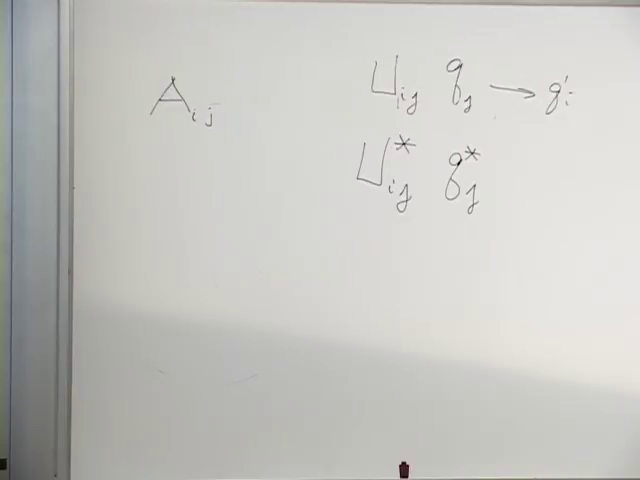
\includegraphics[width=0.62\textwidth]{lecture_05_figure_03.png}\caption{기본 표현의 변환과 그 복소켤레인 반삼중항 표현의 변환.}\lectureframe{00:18:47}\end{figure}

\begin{classroomqa}\audiencequestion{\(U\) 행렬은 몇 개입니까-- 일곱 개, 여덟 개, 아홉 개입니까?
\lecturetimestamp{00:19:37}}\lecturerresponse{군의 원소 \(U\)는 무한히 많습니다. 세는 대상은 독립 생성자의 유한한 개수이며, \(SU(3)\)의 경우 여덟 개입니다. 일반적인 \(3\times3\) 행렬에는 행렬 성분 자리가 아홉 개 있지만, 특수 유니터리 조건 때문에 연속적인 방향은 여덟 개만 남습니다.}\end{classroomqa}

글루온 장은 흔적이 없는 행렬 \(A_{ij}\)로 쓸 수 있다. 한 지표는 쿼크처럼, 다른 지표는 반쿼크처럼 변환하므로 색 구조는 다음과 같다.
\begin{equation}
\boldsymbol 3\otimes\bar{\boldsymbol 3}
=\boldsymbol 1\oplus\boldsymbol 8.
\end{equation} 양자색역학은 흔적이 없는 팔중항을 취하고,
\begin{equation}
A_{ii}=\operatorname{tr}A=0,
\end{equation} 단일항은 제외한다. 그래서 양자색역학에는 아홉 개가 아니라 글루온 여덟 개가 있다. 더 일반적으로 \(SU(N)\)에는
\begin{equation}
N^2-1
\end{equation}개의 생성자와 같은 수의 게이지 보손 장이 있다.

광자는 전기 \(U(1)\)에 대해 중성이다. 전자의 위상을 회전시켜도 광자가 다른 광자로 바뀌지는 않는다. 글루온은 다르다. 글루온은 색과 반색을 띠므로 수반 표현으로 변환한다. 예를 들어 빨강--반파랑 조합은 색 하나와 반색 하나를 포함하지만 색 단일항은 아니다.

\subsection{지표의 흐름과 자기 상호작용}

지표를 따라가면 상호작용 규칙을 읽을 수 있다. 개략적으로 색 \(i\)을 가진 쿼크는 색 \(j\)을 가진 쿼크로 바뀌면서 이에 대응하는 색 흐름을 지닌 글루온을 방출할 수 있다.
\begin{equation}
q_i\longrightarrow q_j+A_{ij}.
\label{eq:l5-quark-gluon-vertex}
\end{equation} \(i\)와 \(j\)의 정확한 위치는 화살표 관례에 따라 달라진다. 불변인 내용은 꼭짓점에 들어오는 모든 지표가 다른 선을 통해 이어져야 한다는 점이다. 색 지표가 사라지는 일은 없다.

이 규칙은 모든 \(SU(N)\) 게이지 이론에 적용된다. 기본 표현의 물질은 지표 하나를, 반기본 표현의 물질은 켤레 지표 하나를 가지며, 게이지 보손은 각각 하나씩 가진다. 물리적 명칭은 달라질 수 있지만 지표 구조는 그대로다.

글루온 자체가 색을 띠기 때문에 다른 글루온을 방출할 수 있다. \(A_{ij}\) 글루온은 중간 지표 \(k\)를 거쳐 개략적으로 다음과 같이 분열할 수 있다.
\begin{equation}
A_{ij}\longrightarrow A_{ik}+A_{kj}.
\label{eq:l5-three-gluon-index}
\end{equation} 이는 완전한 양--밀스 꼭짓점은 아니지만 색 흐름을 보여 준다. 통상적인 전기역학에서 광자에는 이와 비슷한 일이 일어나지 않는다. 따라서 글루온은 글루온에 힘을 가하며, 비아벨 장 동역학은 맥스웰의 선형 이론보다 훨씬 복잡하다.

정성적인 결과 가운데 하나는 가둠이다. 색 선속선은 끝날 수 없으며, 선속선 사이의 자기상호작용은 쿼크와 반쿼크를 잇는 관을 만든다. 이 관은 길이 단위당 거의 일정한 에너지를 지닌다.
\begin{equation}
V(R)\simeq \sigma R.
\end{equation} 따라서 양 끝을 더 멀리 당기면 색을 띤 입자를 자유롭게 풀어 주는 대신 에너지가 더 저장된다. 이것이 끈적한 접착제라는 그림이다. 장 자체가 색을 띤 구성 요소들이 자유 입자로 빠져나오지 못하게 한다.

\section{결합 상수와 강함 또는 약함의 의미}

\subsection{방출 진폭으로서의 전하}

게이지 이론에는 여전히 결합 상수가 필요하다. 양자전기역학에서 전자 전하 \(e\)는 전자--광자 꼭짓점에 해당하는 계수다. 이는 진폭이며, 확률은 진폭의 제곱이다. 작동상의 의미를 보려면 음극선관에서 빠른 전자를 갑자기 멈춘다고 생각해 보자. 광자를 복사할 확률은 \(e^2\)에 비례하며, 관례적인 인자들은 미세구조 상수에 포함된다.
\begin{equation}
\alpha=\frac{e^2}{4\pi\hbar c}
\simeq \frac{1}{137}.
\label{eq:l5-alpha}
\end{equation} 자연 단위계 \(\hbar=c=1\)에서는 결합이 무차원이다. 기본 입자의 방출 척도가 일 퍼센트 정도이므로 섭동론적 의미에서 전자기력은 약하다. 멈춘 전자 대부분이 각각 고에너지 광자를 쏟아내는 것은 아니다.

\subsection{자연 단위계에서 에너지, 시간, 거리의 관계}

다음과 같이 놓자.
\begin{equation}
c=1,
\qquad
\hbar=1.
\end{equation} 그러면 시간과 거리는 같은 단위를 갖고 에너지는 역단위를 갖는다.
\begin{equation}
E=\hbar\omega\longrightarrow E=\omega\sim\frac1t,
\qquad
x\sim t\sim\frac1E.
\end{equation} 큰 에너지는 짧은 거리와 짧은 시간을 탐침한다.

대략적인 감을 잡기 위해,
\begin{equation}
1\ {\rm eV}^{-1}
=\frac{\hbar c}{1\ {\rm eV}}
\simeq 1.97\times10^{-7}\ {\rm m}.
\end{equation} 따라서 원자 길이인 \(10^{-10}\ {\rm m}\)는 대략 역킬로전자볼트에 해당한다. 이는 정밀 분광학에 쓰이는 변환값이 아니라 크기 정도를 나타내는 환산이다.

\subsection{원자 내부의 계층 구조}

전형적인 원자에 대해 다음과 같이 잡자.
\begin{equation}
R_{\rm atom}\sim10^{-10}\ {\rm m}.
\end{equation} 빛이 이 거리를 가로지르는 데 걸리는 시간은
\begin{equation}
t_{\rm transit}^{\rm atom}\sim10^{-18}\ {\rm s}.
\end{equation}이다. 하지만 가벼운 원자에서 전자는 빛의 속도보다 훨씬 느린 속도로 움직인다. 보어 그림에서는 \(v/c\sim\alpha\)이므로 전형적인 궤도 주기는 더 길다.
\begin{equation}
t_{\rm orbit}^{\rm atom}\sim10^{-16}\ {\rm s}.
\end{equation}

들뜬 원자가 복사하는 데는 그보다 더 오래 걸린다.
\begin{equation}
t_{\rm decay}^{\rm atom}\sim10^{-9}\ {\rm s}
\end{equation} 이는 강의에서 크기를 가늠하기 위해 제시한 대략적인 추정값이다. 물리적 그림에는 두 가지 억제가 있다. 전자기력은 크지 않은 가속만 일으키며, 가속하는 전자에는 \(\alpha\)로 정해지는 또 다른 작은 방출 확률이 있다. 따라서 작은 미세구조 상수는 통과 시간, 궤도 시간과 복사 붕괴 시간 사이에 계층 구조를 만든다.

\subsection{하드론에는 계층 구조가 없다}

하드론은 쿼크와 글루온으로 이루어진 원자와 비슷한 결합계지만, 그 크기는 훨씬 작다.
\begin{equation}
R_{\rm hadron}\sim10^{-15}\ {\rm m},
\qquad
t_{\rm transit}^{\rm hadron}\sim10^{-23}\ {\rm s}.
\end{equation} 쿼크는 하드론을 가로지르는 데 거의 같은 시간 규모가 걸리며, 강하게 붕괴하는 들뜬 하드론의 수명도 대략 다음과 같다.
\begin{equation}
t_{\rm orbit}^{\rm hadron}
\sim t_{\rm decay}^{\rm hadron}
\sim10^{-23}\ {\rm s}.
\end{equation} 충격을 받은 하드론은 인과율이 허용하는 거의 가장 빠른 속도로 진동하고 파이온을 방출할 수 있다. 원자 내부에서처럼 일곱 자릿수 또는 아홉 자릿수의 차이는 없다.

\begin{classroomqa}\audiencequestion{특수상대성이론에 따르면 하드론은 빛이 가로지르는 시간보다 훨씬 빠르게 붕괴할 수 없다고 봐도 됩니까?
\lecturetimestamp{00:47:15}}\lecturerresponse{크기 정도의 한계를 표현하는 타당한 방식입니다. 강한 붕괴는 계의 크기가 허용하는 만큼 빠르게 일어납니다. 이를 늦추는 작은 결합이나 그 밖의 큰 억제 요인이 없습니다.}\end{classroomqa}

따라서 이에 대응하는 강한 결합은 \(\alpha\)보다 훨씬 크다. 강의에서는 하드론 척도의 예시로
\begin{equation}
\alpha_{\rm QCD}\sim0.2,
\end{equation}를 제시하는데, 이는 \(1/137\)보다 일에 훨씬 가깝다. 이것이 \emph{강한 상호작용}이라는 옛 명칭의 동역학적 기원이다.
\editorialnote{양자색역학의 결합은 에너지에 따라 달라지므로 \(\alpha_s\)는 하나의 고정된 값이 아니다. 제시된 값은 강의의 의도에 맞춘 척도 의존적인 예시값이다.}

\begin{classroomqa}\audiencequestion{강한 상호작용의 유사한 양을 그냥 강한 힘의 상수라고 부릅니까?
\lecturetimestamp{00:48:17}}\lecturerresponse{관례적으로 \(\alpha_{\rm QCD}\)라고 부르며, 더 흔히는 \(\alpha_s\)라고 합니다. 전자기 쪽은 보통 그냥 \(\alpha\)라고 부르지만, 같은 논의에서 둘 다 나타날 때는 \(\alpha_{\rm QED}\)를 쓸 수도 있습니다.}\end{classroomqa}

\begin{classroomqa}\audiencequestion{논문에서는 전자기 결합의 맨값과 측정된 차폐값을 구별합니까?
\lecturetimestamp{00:48:38}}\lecturerresponse{그렇습니다. 맨결합과 재규격화된 결합이라는 표현을 씁니다. 진공 편극 때문에 유효 결합은 측정하는 척도에 따라 달라집니다.}\end{classroomqa}

\section{약붕괴의 수수께끼}

약한 상호작용은 붕괴 시간이 매우 길다는 점에서 이름이 붙었다. 대체로 강한 붕괴보다 느리고 원자 복사보다 느릴 수도 있다. 가장 오래된 사례는 핵 베타 붕괴다.

\subsection{중성자의 베타 붕괴}

자유 중성자는 다음 과정을 통해 붕괴한다.
\begin{equation}
n\longrightarrow p+e^-+\bar\nu_e.
\label{eq:l5-neutron-decay-intro}
\end{equation} 강의에서는 수명을 대략 십이 분으로 잡는데, 이는 \(10^{-23}\ {\rm s}\)와 비교하면 터무니없이 길다. 이 논증에서는 현대의 정밀한 측정값이 중요하지 않다.

느린 이유 중 일부는 운동학에 있다. 대략,
\begin{equation}
\begin{aligned}
m_n&\simeq940\ {\rm MeV},
&
m_p&\simeq939\ {\rm MeV},
\\
m_e&\simeq0.5\ {\rm MeV}.
\end{aligned}
\end{equation} 중성자 정지 에너지 가운데 운동 에너지로 쓸 수 있는 부분은 아주 작다. 중성자 질량이 최종 입자들의 정지 질량 합보다 작다면 붕괴는 불가능했을 것이다. 문턱값을 무한소만큼 넘는 정도라면 이용 가능한 위상 공간이 아주 작아 붕괴가 느릴 것이다. 하지만 위상 공간만으로는 수명이 분 단위인 이유를 설명할 수 없다.

\subsection{하전 파이온은 문턱에너지라는 변명을 무력화한다}

다음 과정도 생각해 보자.
\begin{equation}
\pi^-\longrightarrow e^-+\bar\nu_e
\end{equation} 그리고 그 전하켤레 과정도 있다. 파이온은 전자 채널의 문턱값보다 훨씬 높은 에너지를 지니지만, 약한 붕괴 수명은 여전히 나노초 정도로, 하드론의 \(10^{-23}\)초 정도와는 다르다. 뮤온을 포함하는 비슷한 채널도 곧 중요해진다. 따라서 이 수수께끼는 중성자의 질량이 거의 축퇴해 있다는 우연 때문이 아니라 약한 상호작용 자체에 내재한다.

\editorialnote{하전 파이온의 수명은 약 \(26\ {\rm ns}\)이며, 지배적인 채널은 \(\pi^-\to\mu^-\bar\nu_\mu\)이다. 전자 채널은 헬리시티 억제를 받는다. 강의에서는 입자 수지가 가장 간단한 전자 채널을 먼저 사용한 뒤, 지배적인 뮤온 채널을 다시 다룬다.}

베타 붕괴라는 용어는 방출된 전자를 베타선이라 부르던 역사에서 유래했다. 파이온과 중성자 사례는 운동학이 크게 다르지만 같은 하전 전류 상호작용을 포함한다.

\section{쿼크와 렙톤 표}

\subsection{색은 세로 방향으로 작용한다}

여섯 쿼크 맛을 짝지은 세 열에 배열하고,
\begin{equation}
(u,d),\qquad(c,s),\qquad(t,b),
\end{equation} 각 쿼크를 빨강, 초록, 파랑으로 복제해 별도의 행에 놓자. 색 \(SU(3)\)은 세로 방향으로 작용한다. 업 쿼크의 빨강, 초록, 파랑 상태를 서로 변환하며 다운, 참, 기묘, 톱, 바닥 쿼크에도 같은 색 회전을 동시에 적용한다. 업 쿼크를 다운 쿼크로 바꾸지는 않는다.

\subsection{약한 아이소스핀은 가로 방향으로 작용한다}

약한 대칭은 다른 방향으로 작용한다. 이웃한 각 쌍을 서로 섞는다.
\begin{equation}
Q_1=\begin{pmatrix}u\\d\end{pmatrix},
\qquad
Q_2=\begin{pmatrix}c\\s\end{pmatrix},
\qquad
Q_3=\begin{pmatrix}t\\b\end{pmatrix}.
\label{eq:l5-quark-doublets}
\end{equation} 업형 쿼크의 전하는 \(+2/3\)이고 다운형 쿼크의 전하는 \(-1/3\)이므로 각 쌍을 가로질러 전하가 한 단위만큼 바뀐다.
\editorialnote{원문에서는 잠시 다운 쿼크의 전하가 \(-2/3\)라고 말한다. 앞뒤의 뺄셈과 이후의 모든 과정에는 여기서 사용한 표준값 \(-1/3\)이 필요하다.}

대칭이 이중항에 작용하므로 자연스러운 군은 \(SU(2)\)이다. 각 쿼크 이중항의 모든 색 상태에 작용하면서 색은 바꾸지 않는다.

색을 띠지 않아 글루온과 상호작용하지 않는 네 번째 입자 행도 있는데, 렙톤이다. 렙톤은 세 개의 이중항을 이룬다.
\begin{equation}
L_e=\begin{pmatrix}\nu_e\\e^-\end{pmatrix},
\qquad
L_\mu=\begin{pmatrix}\nu_\mu\\\mu^-\end{pmatrix},
\qquad
L_\tau=\begin{pmatrix}\nu_\tau\\\tau^-\end{pmatrix}.
\label{eq:l5-lepton-doublets}
\end{equation} 중성미자는 전기적으로 중성이고 전자, 뮤온, 타우의 전하는 \(-1\)이다. 여기서도 두 구성원은 전하가 한 단위 차이 난다. 세대가 다른 업형 또는 다운형 쿼크가 같은 전하 배열을 되풀이하듯, 전자, 뮤온, 타우도 같은 게이지 양자수를 가지지만 질량은 서로 다르다.

\begin{figure}[htbp]\centering
\includegraphics[width=0.82\textwidth]{lecture_05_figure_05.png}\caption{칠판 표: 색은 빨강, 파랑, 초록 행 사이에서 작용하고, 약한 \(SU(2)\)은 짝지어진 맛 열과 렙톤 행을 연결한다.}\lectureframe{01:03:35}\end{figure}

렙톤을 네 번째 색이라고 부르는 것은 이 단계에서는 비유일 뿐이다. 렙톤은 약한 이중항 표에서 네 번째 행을 차지하지만, 통상적인 양자색역학 \(SU(3)\)은 쿼크를 렙톤으로 변환하지 않는다.

\section{하전 약 보손의 구성}

\subsection{하전 보손의 양자수}

게이지 보손은 이중항의 한 구성원에서 다른 구성원으로 옮기는 데 필요한 변환 성질을 지닌다. 렙톤 쌍 \(e^-\bar\nu_e\)부터 보자. 이 쌍은 전하 \(-1\)를 가지므로, 이에 대응하는 하전 게이지 보손을 \(W^-\)라고 부른다.
\begin{equation}
W^-\sim e^-\bar\nu_e.
\end{equation} 다운 쿼크와 반업 쿼크에서도 같은 양자수가 나온다.
\begin{equation}
W^-\sim d\bar u.
\end{equation} 기호 \(\sim\)는 관련된 게이지 양자수가 같다는 뜻이다. \(W\)가 문자 그대로 이 입자들의 결합 상태라는 뜻은 아니다. 반입자에는 켤레 조합이 대응한다.
\begin{equation}
W^+\sim e^+\nu_e\sim\bar d u.
\end{equation}

하전 약한 꼭짓점에는 다음 과정이 포함된다.
\begin{align}
e^-&\longrightarrow\nu_e+W^-,
&
\mu^-&\longrightarrow\nu_\mu+W^-,
\label{eq:l5-lepton-w}\\
d&\longrightarrow u+W^-,
&
s&\longrightarrow c+W^-,
\label{eq:l5-quark-w}
\end{align} 운동학적으로 허용되는 경우에는 삼세대의 유사한 전이도 포함된다. 게이지 보손은 이중항에 대한 대칭의 수평 혼합과 같은 혼합을 동역학적으로 일으킨다.

\begin{classroomqa}\audiencequestion{전하 보존으로 방출되는 보손의 전하는 \(-1\)로 정해집니다. 그런데 전자, 다운 쿼크, 기묘 쿼크의 전이가 모두 같은 입자를 포함해야 하는 이유는 무엇입니까?
\lecturetimestamp{01:12:56}}\lecturerresponse{이는 공통 약한 대칭에 담긴 실험적 사실입니다. 자연이 각 계열마다, 또는 쿼크와 렙톤에 서로 다른 \(W\)형 보손을 일관되게 배정하는 것도 가능했습니다. 하지만 실제로는 하나의 \(SU(2)\)이 모든 이중항에 동시에 작용하며, 같은 하전 게이지 보손이 이 모든 전이를 매개합니다.}\end{classroomqa}

\subsection{정점을 읽고 역방향으로 읽기}

하나의 꼭짓점은 일련의 과정을 나타낸다. 들어오는 선을 나가는 선으로 바꾸면 입자가 반입자로 바뀌며, \(W^-\) 선의 방향을 뒤집으면 \(W^+\)가 된다. 따라서 전하, 운동량과 관련된 모든 양자수를 일관되게 추적하는 한, 꼭짓점을 방출, 흡수, 붕괴, 소멸 또는 역반응으로 읽을 수 있다.

\begin{classroomqa}\audiencequestion{이 약한 꼭짓점에서 화살표와 선의 방향을 뒤집어도 됩니까?
\lecturetimestamp{01:14:51}}\lecturerresponse{그렇습니다. 선을 최종 상태에서 초기 상태로 또는 그 반대로 교차해 옮길 수 있지만, 이때 입자는 반입자로 바뀝니다. 따라서 같은 국소 꼭짓점이 방향이 서로 다른 여러 반응을 나타냅니다.}\end{classroomqa}

\begin{classroomqa}\audiencequestion{\(W^-\)에 기묘 쿼크와 참 쿼크 선을 그리면 보손이 문자 그대로 기묘 쿼크와 반참 쿼크의 결합 상태라는 뜻입니까?
\lecturetimestamp{01:15:43}}\lecturerresponse{아닙니다. 선으로 표시한 것은 \(W^-\)가 그 두 열 사이의 양자수 변화를 운반한다는 뜻일 뿐입니다. 다이어그램을 붕괴 과정으로 읽을 경우 충분한 에너지를 가진 \(W^-\)가 기묘 쿼크와 반참 쿼크를 만들 수는 있지만, 그 보손이 이들로 이루어진 것은 아닙니다.}\end{classroomqa}

\begin{classroomqa}\audiencequestion{전자와 반중성미자가 \(W\)를 만들고, 이것이 쿼크 쌍을 생성할 수 있습니까?
\lecturetimestamp{01:17:22}}\lecturerresponse{그렇습니다. 질량중심 에너지가 충분하면 초기 렙톤들이 하전 전류 중간 상태를 만들고, 그 상태가 허용된 쿼크 채널을 통해 나타날 수 있습니다. 두 꼭짓점은 붕괴 과정에서 사용한 것과 같으며, 방향만 다르게 읽은 것입니다.}\end{classroomqa}

\subsection{빠진 세 번째 보손}

\(SU(2)\)군에는 생성자가 셋이므로 게이지 장도 셋이다. 지금까지는 \(W^+\)와 \(W^-\)만 나타냈다. 전기적으로 중성인 세 번째 장은 전자--양전자 및 중성미자--반중성미자 양자수와 같은 대각 조합에 대응해야 한다. 이 장은 의도적으로 배경에 남겨 둔다. 이 장과 물리적인 \(Z\) 보손 및 광자의 관계를 알려면 뒤에서 다룰 약전자기 혼합이 필요하다.

\begin{classroomqa}\audiencequestion{약한 힘과 강한 힘은 역사적으로 서로 다른 시기에 의심받았습니까?
\lecturetimestamp{01:24:11}}\lecturerresponse{두 힘의 실험적 기원은 초기 방사능 연구에서 함께 나타났습니다. 알파 붕괴는 핵물리와 강한 상호작용 물리의 단서를 드러냈고, 베타 붕괴는 약한 상호작용을 드러냈으며, 감마 붕괴에서는 전자기 광자가 방출되었습니다. 현대적 장 이론이 나오기 훨씬 전인 베크렐 시대에 이미 세 가지 단서가 모두 나타났습니다.}\end{classroomqa}

\section{하전 전류 붕괴의 풀이 예}

\subsection{파이온 붕괴}

음전하 파이온의 원자가 쿼크 구성은 다음과 같다.
\begin{equation}
\pi^-=d\bar u.
\end{equation} 이 양자수는 \(W^-\)로 소멸할 수 있고, 이어서 하전 렙톤과 그에 대응하는 반중성미자를 만들 수 있다.
\begin{align}
\pi^-&\longrightarrow W^{-*}
\longrightarrow e^-+\bar\nu_e,
\label{eq:l5-pion-electron}\\
\pi^-&\longrightarrow W^{-*}
\longrightarrow \mu^-+\bar\nu_\mu.
\label{eq:l5-pion-muon}
\end{align} 별표는 중간 \(W\)가 가상 입자임을 나타낸다. 두 번째 채널이 지배적이다.

\begin{figure}[htbp]\centering
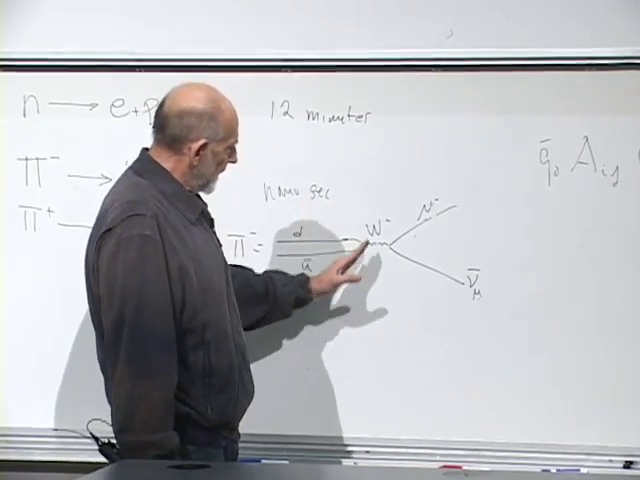
\includegraphics[width=0.72\textwidth]{lecture_05_figure_04.png}\caption{\(d\bar u\) 파이온이 가상 \(W^-\)로 소멸한 뒤 하전 렙톤과 이에 대응하는 반중성미자가 생성된다.}\lectureframe{01:19:38}\end{figure}

\begin{classroomqa}\audiencequestion{시간 방향을 세로가 아니라 가로로 그렸는데도 정말 파인만 다이어그램입니까?
\lecturetimestamp{01:20:21}}\lecturerresponse{그렇습니다. 페이지에서 시간을 어느 방향으로 나타낼지는 관례입니다. 한 방향을 시간으로 정하고 모든 화살표를 일관되게 해석하면, 그림은 동일한 상호작용 정보를 담습니다.}\end{classroomqa}

\begin{classroomqa}\audiencequestion{이 다이어그램을 비가역적인 일방향 붕괴라기보다 가역적인 화학 반응처럼 볼 수 있을까요?
\lecturetimestamp{01:21:35}}\lecturerresponse{역과정도 허용됩니다. 진공에서 생성된 파이온은 붕괴 생성물들이 서로 멀어져 보통은 다시 결합하지 않기 때문에 붕괴합니다. 하지만 뮤온과 반중성미자를 적절한 에너지와 운동량으로 함께 충돌시키면, 역상호작용을 통해 파이온을 형성할 진폭은 영이 아닙니다.}\end{classroomqa}

\subsection{에너지와 가상 중간 상태}

정지한 파이온에 대해,
\begin{equation}
m_\pi\simeq140\ {\rm MeV},
\qquad
m_\mu\simeq106\ {\rm MeV},
\qquad
m_\nu\approx0
\end{equation} 여기서 중요한 정밀도 수준에서는 이 정도다. 남은 에너지는 나가는 입자들의 운동 에너지가 된다. 운동량 보존에 따르면
\begin{equation}
\boldsymbol p_\mu+\boldsymbol p_{\bar\nu}=0,
\end{equation} 따라서 파이온 정지 좌표계에서 두 입자는 서로 반대 방향으로 날아간다.

\begin{classroomqa}\audiencequestion{\(W\)가 파이온보다 훨씬 무거운데 에너지가 어떻게 보존될 수 있습니까?
\lecturetimestamp{01:25:08}}\lecturerresponse{질량 껍질 위에 있어야 하는 것은 초기 입자와 최종 입자뿐입니다. 각 꼭짓점에서 사차원 운동량은 보존되지만 내부의 가상 선은 \(E^2=\boldsymbol p^2+m_W^2\)을 만족할 필요가 없습니다. 질량 껍질에서 벗어난 정도가 클수록 전파자가 과정을 더 강하게 억제합니다.\editorialnote{강의에서는 전통적인 에너지--시간 불확정성 표현을 사용하며 중간 상태가 짧은 시간 동안 에너지를 위반할 수 있다고 말한다. 더 정확한 현대적 설명은 답변에 제시된 것이다. 에너지와 운동량은 보존되지만 내부의 가상 선은 실제 입자의 질량 껍질 조건을 만족할 필요가 없다.}}\end{classroomqa}

\subsection{뮤온 붕괴}

뮤온은 먼저 가상 \(W^-\)를 방출하여 뮤온 중성미자로 바뀔 수 있다.
\begin{equation}
\mu^-\longrightarrow\nu_\mu+W^{-*}.
\end{equation} 이어서 가상 보손은 전자와 전자 반중성미자를 만든다.
\begin{equation}
\mu^-\longrightarrow
\nu_\mu+e^-+\bar\nu_e.
\label{eq:l5-muon-decay}
\end{equation} 이는 순수한 렙톤 과정이다. 뮤온은 전자보다 질량이 약 이백 배 크므로 최종 입자들의 정지 질량을 제하고도 운동 에너지로 쓸 에너지가 충분히 남는다.

\begin{figure}[htbp]\centering
\includegraphics[width=0.72\textwidth]{lecture_05_figure_06.png}\caption{가상 하전 약한 보손을 통한 뮤온 붕괴.}\lectureframe{01:29:24}\end{figure}

\begin{classroomqa}
\audiencequestion{전자와 함께 방출되는 중성 입자는 반중성미자인가요?
\lecturetimestamp{01:29:06}}
\lecturerresponse{그렇습니다. 완전한 최종 상태에는 뮤온 중성미자 하나, 전자 반중성미자 하나, 전자가 들어 있습니다. 맛을 나타내는 표지를 붙이면 두 중성 입자를 혼동하지 않을 수 있습니다.}
\end{classroomqa}

전자는 뮤온보다 가볍기 때문에 진공에서는 이 붕괴를 역으로 일으킬 수 없습니다. 타우는 더 무거워서 유사한 약한 상호작용 채널을 통해 붕괴할 수 있습니다. 여기서 안정성은 기초가 되는 꼭짓점의 차이 때문이 아니라, 부분적으로는 질량의 순서가 우연히 그렇게 정해져 있기 때문입니다.

\begin{classroomqa}
\audiencequestion{선형 가속기는 사실상 전자의 질량을 증가시켜, 그렇지 않으면 금지되는 반응을 반대 방향으로 일으키는 건가요?
\lecturetimestamp{01:30:23}}
\lecturerresponse{전자 고유 정지 질량을 바꾸지는 않지만 운동 에너지를 공급합니다. 충분한 질량중심 에너지가 있으면 더 무거운 최종 입자를 생성할 수 있으므로, 질량을 충돌에 이용 가능한 에너지로 바꾸어 말하면 제안하신 물리적 발상은 맞습니다.}
\end{classroomqa}

\subsection{쿼크 수준에서 본 중성자 베타 붕괴}

중성자와 양성자의 원자가 쿼크 조성은 다음과 같습니다.
\begin{equation}
n=udd,
\qquad
p=uud.
\end{equation}
중성자의 다운 쿼크 하나는 하전 전류 전이를 일으켜
\begin{equation}
d\longrightarrow u+W^{-*},
\end{equation}
\(udd\)에서 \(uud\)으로 바뀝니다. 이어서 가상 보손이 붕괴합니다.
\begin{equation}
W^{-*}\longrightarrow e^-+\bar\nu_e.
\end{equation}
두 꼭짓점을 결합하면 다음 과정이 재현됩니다.
\begin{equation}
n\longrightarrow p+e^-+\bar\nu_e.
\end{equation}

반대 방향의 쿼크 전이 \(u\to d+W^+\)가 일어나면 다운 쿼크 세 개로 이루어진 바리온이 생성되지만, 자유 중성자가 생성하기에는 그 상태의 질량이 너무 큽니다. 실제로 일어나는 다운에서 업으로의 전이는 에너지상 허용되는 경로입니다.

\begin{classroomqa}
\audiencequestion{중성자가 대신 양성자, 뮤온, 그리고 이에 대응하는 반중성미자로 붕괴할 수 있나요?
\lecturetimestamp{01:32:38}}
\lecturerresponse{정지해 있는 자유 중성자에서는 불가능합니다. 중성자--양성자 질량 차이는 뮤온 질량보다 훨씬 작습니다. 충돌이나 여기로 충분한 에너지를 더 공급하면, 같은 약한 상호작용 꼭짓점이 뮤온을 생성하는 채널에 관여할 수 있습니다. 금지되는 이유는 운동학적 제약이지, 상호작용이 없어서가 아닙니다.}
\end{classroomqa}

\section{아직 설명되지 않은 억제}

하전 약한 상호작용 꼭짓점으로 어떤 과정이 일어날 수 있는지는 설명되지만, 그 과정이 왜 그렇게 느린지는 아직 설명되지 않습니다. 약한 상호작용 결합이 유난히 작기 때문이라고 답하고 싶을 수도 있습니다. 그러나 그 답은 틀렸습니다. 무차원 약한 게이지 결합은 대략 전자기 결합과 비슷한 크기입니다. 억제의 원인은 다른 데서 찾아야 합니다.

빠진 요소는 가상 입자 전파자에서 이미 드러납니다. \(W\)은 매우 무겁습니다. \(m_W\)보다 훨씬 낮은 에너지에서는 하전 전류 진폭이 대략 \(1/m_W^2\)의 거듭제곱에 따라 억제됩니다. 힉스 메커니즘과 전약 대칭 깨짐을 통해 게이지 보손이 질량을 얻는 방식을 설명한 뒤 이 연결을 전개하겠습니다.
\editorialnote{이 강의에서는 이 문제를 다음 강의에서 다룰 수수께끼로 남겨 둡니다. 무거운 \(W\)에 대한 설명은 앞으로 이어질 내용을 미리 연결하기 위해 여기에 포함했으며, 이 강의에서 그 유도가 이루어졌다는 뜻은 아닙니다.}

\begin{classroomqa}
\audiencequestion{이 이론이 이러한 대칭성을 가진다고 할 때, 해당 변환에 대해 라그랑지안이 불변이라는 뜻인가요?
\lecturetimestamp{01:34:14}}
\lecturerresponse{맞습니다. 이론이 그 대칭성을 가진다는 말은 해당 변환에 대해 라그랑지안, 또는 동등하게 작용이 불변이라는 뜻을 줄여 표현한 것입니다. 라그랑지안 전체를 쓰는 일은 뒤로 미룬 것이지, 대칭성의 정의를 다른 것으로 바꾼 것이 아닙니다.}
\end{classroomqa}

이제 논의의 흐름이 완성되었습니다. 맥스웰 이론은 원형을 제시하고, 양자색역학은 비아벨 게이지 보손이 전하를 지니고 교환하는 방식을 보여 줍니다. 결합 상수는 원자 규모와 강입자 규모의 시간 척도 차이를 설명합니다. 그리고 약한 \(SU(2)\)은 쿼크와 렙톤을 \(W^\pm\)으로 묶어 줍니다. 이제 남은 과제는 기초 결합이 특별히 작지 않은데도 게이지 매개 과정이 실제로는 왜 약한지 이해하는 것입니다.
\chapter{질량을 가진 약한 상호작용의 교환, 가상 입자, 대칭 깨짐}

표준모형의 군은 페르미온 표에서 허용되는 변환들의 집합으로 보면 훨씬 덜 신비롭게 다가온다. 색 변환은 빨강, 초록, 파랑 사이에서 세로 방향으로 움직인다. 전하를 띤 약한 변환은 쿼크와 렙톤 이중항 안에서 가로 방향으로 움직인다. 전자기 위상 변환은 세 번째 연산을 제공한다. 이에 대응하는 게이지 보손은 대칭을 찾은 뒤에 덧붙인 장식이 아니다. 게이지 보손을 방출하면 대칭의 생성자가 기술하는 것과 같은 상태 변화가 물리적으로 일어난다.

이 관찰을 바탕으로 이번 강의의 핵심 질문을 제기할 수 있다. 약한 상호작용의 꼭짓점 결합은 전자기 상호작용의 꼭짓점 결합과 비슷한 크기인데도, 베타 붕괴는 전형적인 강한 상호작용 과정이나 전자기 과정에 비해 엄청나게 느리다. 여기에 빠진 요소는 전파다. 운동량이 낮을 때 질량이 있는 \(W\)를 교환하면 진폭에 대략 \(1/m_W^2\)의 인자가 곱해진다. 먼저 거리 공간에서, 다음으로 운동량 공간에서 이 설명을 전개하고, 실재 입자와 가상 입자에 관한 긴 논의를 거쳐 마지막으로 자발적 대칭 깨짐의 첫 정성적 모형을 살펴보겠다.

\section{페르미온 표에서 게이지 대칭 읽기}

\subsection{색은 세로 방향으로 작용한다}

여섯 가지 쿼크 맛을 세 약한 상으로 배열하고,
\begin{equation}
  (u,d),\qquad(c,s),\qquad(t,b),
\end{equation}
각 쿼크에 빨강, 초록 또는 파랑의 색 표지를 붙이자. 이렇게 얻은 쿼크 표에는 색 행이 세 개, 맛 열이 여섯 개 있다. 색 \(SU(3)\)은 어느 한 맛 열 안의 세 항목을 서로 섞는다. 예를 들어 한 생성자는 빨간 업 쿼크를 초록 업 쿼크로 바꿀 수 있다. 입자 언어로 같은 작용을 말하면, 보상하는 색과 반색을 지닌 글루온의 방출이 동반된다.

같은 색 변환은 모든 맛에 작용해야 한다. 빨간 업 쿼크를 초록 업 쿼크로 바꾸는 글루온은 빨간 톱 쿼크를 초록 톱 쿼크로 바꾸는 글루온과 같은 종이다. 진정한 대칭 작용은 1세대에만 적용되고 나머지 세대는 무시하지 않는다. 따라서 색 변환은 세로 방향으로 일어나며 보편적으로 작용한다.
\begin{equation}
  q_r\longleftrightarrow q_g\longleftrightarrow q_b,
  \qquad q\in\{u,d,c,s,t,b\}.
\end{equation}
색은 바꾸지만 맛은 바꾸지 않는다.

이것은 게이지 군과 그 게이지 보손 사이의 전형적인 관계다. 무한소 생성자는 상태들 사이의 변환을 기술하며, 이에 대응하는 보손을 방출하거나 흡수하면 그 변환이 물리적 과정으로 구현된다.

\subsection{약한 변환은 가로 방향으로 작용한다}

전하를 띤 약한 상호작용은 다른 방향으로 작용한다. 업형 쿼크는 색을 바꾸지 않은 채 전하를 띤 약한 보손을 방출하고 다운형 짝으로 바뀔 수 있다.
\begin{equation}
  u_b\longrightarrow d_b+W^+.
\end{equation}
정확히 같은 \(W^+\)가
\begin{equation}
  c_g\longrightarrow s_g+W^+,
  \qquad
  t_r\longrightarrow b_r+W^+.
\end{equation}
에서도 일어난다. \(r,g,b\) 표지는 이 과정에서 바뀌지 않는다. 글루온은 표를 가로질러 움직이지 않으며, 전하를 띤 \(W\) 보손은 색 표에서 세로 방향으로 움직이지 않는다.

전자기 위상 대칭 \(U(1)\)을 더하면 모든 전하를 띤 장에 위상이 붙는다. 우선 생각해 볼 군 구조는 다음과 같다.
\begin{equation}
  SU(3)\times SU(2)\times U(1).
\end{equation}
곱셈 기호는 서로 독립적인 인자임을 뜻한다. 하나는 색에, 하나는 약한 이중항에, 나머지 하나는 위상에 작용한다. 이것은 유용한 대략적 그림이지만, 전약 이론 전체를 나타내지는 않는다.\editorialnote{표준모형의 정확한 게이지 군은 관례적으로 \(SU(3)_c\times SU(2)_L\times U(1)_Y\)라고 쓴다. 약한 \(SU(2)_L\)는 왼손잡이 이중항에만 작용하며, 최종적인 전자기 \(U(1)_{\rm em}\)는 대칭 깨짐 뒤 \(SU(2)_L\times U(1)_Y\)에서 나타난다. 강의에서는 처음에 제시한 마지막 두 인자의 동일시가 아직 완전히 일관되지 않는다고 명시한다. 빠져 있는 카이랄 구조와 전약 구조는 뒤 강의들에서 다룬다.}

\subsection{같은 패턴은 렙톤에도 적용된다}

세 색 행 아래에 색이 없는 렙톤 행을 놓자.
\begin{equation}
\begin{array}{c|cc|cc|cc}
 &u&d&c&s&t&b\\ \hline
Q&+\frac23&-\frac13&+\frac23&-\frac13&+\frac23&-\frac13\\
\text{lepton partner}
 &\nu_e&e^-&\nu_\mu&\mu^-&\nu_\tau&\tau^-\\
Q&0&-1&0&-1&0&-1
\end{array}
\end{equation}
서로 이웃한 각 쌍에서는 전하가 한 단위만큼 다르다. 그래서 같은 전하를 띤 약한 보손이 \(u\)와 \(d\), \(c\)와 \(s\), \(t\)와 \(b\), 그리고 전하를 띤 렙톤과 그 중성미자를 연결할 수 있다. \(W\) 꼭짓점은 해당 양자수와 전하 차이에 따라 작용하며, 페르미온이 쿼크인지 렙톤인지는 따지지 않는다.

\begin{figure}[htbp]\centering
\includegraphics[width=0.88\textwidth]{lecture_06_figure_07.png}\caption{완성된 페르미온 표. 위쪽에는 세 색의 쿼크 행, 아래쪽에는 색이 없는 렙톤 행이 있으며 쿼크의 전하와 세 렙톤 이중항이 보인다.}\lectureframe{00:18:55}\end{figure}

뮤온은 전하와 알려진 내재 양자수가 전자와 같지만, 질량은 약 200배 더 크다. 타우는 그보다도 더 무겁다. 중성미자 질량은 매우 작으며, 이 강의에서 논의할 당시에는 자세히 알려져 있지 않았다. 여기까지는 관측된 세대별 질량 패턴을 설명하는 원리가 아직 나오지 않았다.

\begin{classroomqa}\audiencequestion{렙톤, 바리온, 중간자는 왜 그런 이름으로 불리나요?
\lecturetimestamp{00:19:02}}\lecturerresponse{그리스어 어원은 대략 가벼움, 무거움, 중간을 뜻했다. 질량에 근거한 이 명명법은 오해를 낳게 되었다. 뮤온은 질량이 전자와 양성자의 질량 사이에 있어서 한때 뮤 중간자라고 불렸지만, 상호작용을 보면 파이온보다 전자에 훨씬 가까운 렙톤이다. 오늘날 중간자는 쿼크--반쿼크 하드론을 뜻하며 보손이다. 뮤온은 중간자가 아니다.}\end{classroomqa}

\section{약한 상호작용의 수수께끼}

\subsection{구체적인 하전 전류 과정}

중성자 베타 붕괴를 예시 도식으로 살펴보자. 원자가 쿼크의 구성은 다음과 같다.
\begin{equation}
  n=udd,\qquad p=uud.
\end{equation}
다운 쿼크 하나가 다음 전이를 한다.
\begin{equation}
  d\longrightarrow u+W^-,
\end{equation}
그리고 전하를 띤 보손은 다음 입자들을 만든다.
\begin{equation}
  W^-\longrightarrow e^-+\bar\nu_e.
\end{equation}
두 과정을 합치면,
\begin{equation}
  n\longrightarrow p+e^-+\bar\nu_e.
\end{equation}
나머지 원자가 쿼크 두 개는 구경꾼으로서 그대로 이어진다. 첫 번째 꼭짓점에서 중성자는 양성자로 바뀐다. 두 번째 꼭짓점에서는 렙톤 이중항을 연결하는 것과 같은 약한 상호작용으로 \(W^-\)가 관측되는 전자와 전자 반중성미자로 바뀐다.

\subsection{세 결합, 크게 다른 세 가지 인상}

양자전기역학에서 전자 전하 \(e\)는 꼭짓점 진폭이다. 이를 제곱하면 특징적인 방출 확률을 얻으며, 자연 단위계에서는 통상적인 인자들을 모아 다음과 같이 쓴다.
\begin{equation}
  \alpha=\frac{e^2}{4\pi}\simeq\frac1{137}
\end{equation}
강한 상호작용의 결합은 \(g_s\)이며, 전형적인 하드론 에너지 척도에서 이에 대응하는 \(\alpha_s\)는 대략 \(0.2\)일 수 있다. 이는 \(1/137\)보다 훨씬 크므로 쿼크가 충돌할 때 글루온이 흔히 방출된다.

전하를 띤 약한 결합을 \(g_w\)이라 하자. 그 제곱은 터무니없이 작지 않으며, 여기서 사용하는 크기 정도의 추정으로는 전자기 결합과 비슷하다. 그런데도 자유 중성자는 붕괴하기까지 대략 15분을 기다리는 반면, 강한 붕괴는 하드론이 가로지르는 시간 척도에서 일어날 수 있다. 강의의 역사적 추정에는 더 오래된 대략값인 12분이 쓰였지만, 어느 수치를 택해도 같은 수수께끼가 분명히 드러난다.\editorialnote{현재 측정된 자유 중성자의 평균 수명은 약 \(8.8\times10^2\,{\rm s}\)이며, 주요 측정 방법들 사이에는 여전히 실험적 불일치가 있다. 강의에서 제시한 대략적인 수명은 정밀한 값이 아니라 설명에 쓰이는 시간 척도로 유지한다.}\begin{quote}\(g_w\)이 특별히 작지 않다면 약한 과정은 무엇 때문에 약한가?
\end{quote}

답은 꼭짓점에만 있지 않다. 모든 파인만 도표에는 한 꼭짓점에서 다른 꼭짓점까지 중간 전파를 기술하는 인자인 전파인자도 들어 있다.

\section{거리 공간에서 질량을 가진 전파인자}

\subsection{꼭짓점만으로 도표가 완성되지는 않는다}

베타 붕괴 도표에는 약한 꼭짓점 두 개가 있어 \(g_w\)가 두 번 곱해지고, 그 사이를 잇는 \(W\) 선이 있다. 위치 공간 전파인자를 \(\Delta(x-y)\)라 하자. 여기서 \(x\)는 방출 사건의 위치이고 \(y\)는 흡수 또는 변환 사건의 위치다. 이는 두 사건 사이에서 장의 교란이 전달되는 것과 연관된 진폭 커널이다.

정확한 상대론적 전파인자에는 여기서 필요한 것보다 더 많은 구조가 들어 있다. 정성적으로 중요한 특징은 질량에 대한 의존성이다. 짧은 공간꼴 거리에선 거듭제곱형 특이성을 가지며, 개략적으로 다음과 같다.
\begin{equation}
  \Delta(d)\sim\frac1{d^2}.
\end{equation}
질량이 없는 장에는 거듭제곱 꼬리가 남는다. 반면 질량을 가진 장은 분리가 콤프턴 척도보다 커지면 지수적으로 억제된다. 따라서 그래프는 급격히 아래로 꺾인다.

\subsection{자연 단위계로 꺾이는 지점 찾기}

다음과 같이 놓자.
\begin{equation}
  c=\hbar=1.
\end{equation}
그러면
\begin{equation}
  [m]=[E]=[p]=L^{-1}.
\end{equation}
익숙한 관계를 이용하면 각 등식의 의미를 알 수 있다. \(E=mc^2\)는 질량과 에너지를 연결하고, \(p\,x\)의 차원은 \(\hbar\)의 차원이므로 운동량과 거리는 서로 역수의 단위를 갖는다. 따라서 질량 \(m\)으로 만들 수 있는 유일한 길이 척도는 다음과 같다.
\begin{equation}
  d_m\sim\frac1m.
\end{equation}
상수를 복원하면 콤프턴 파장은
\begin{equation}
  d_m\sim\frac{\hbar}{mc},
\end{equation}
가 된다. 교환 입자가 무거울수록 유효 범위는 짧아진다.

\begin{figure}[htbp]\centering
\includegraphics[width=0.78\textwidth]{lecture_06_figure_02.png}\caption{자연 단위계의 차원과 전파인자의 정성적 감소. 검은 곡선은 거듭제곱 꼬리로 이어지고, 빨간 질량 있는 곡선은 역질량 척도 부근에서 아래로 꺾인다.}\lectureframe{00:27:19}\end{figure}

\begin{figure}[htbp]\centering
\begin{tikzpicture}[x=1.0cm,y=0.9cm]
  \draw[->] (0,0) -- (7,0) node[right] {$d$};
  \draw[->] (0,0) -- (0,5) node[above] {$|\Delta(d)|$};
  \draw[thick]
    plot[smooth] coordinates {(0.45,4.5) (0.9,3.3) (1.6,2.5)
      (2.5,1.9) (3.7,1.45) (5.1,1.12) (6.4,0.9)};
  \draw[thick,red]
    plot[smooth] coordinates {(0.45,4.5) (0.9,3.3) (1.6,2.5)
      (2.5,1.9) (3.2,1.55) (3.7,0.95) (4.2,0.36) (4.8,0.1)};
  \draw[dashed] (3.4,0) -- (3.4,1.4);
  \node at (5.7,1.4) {$m=0$};
  \node[red] at (4.75,0.72) {$m>0$};
  \node[below] at (3.4,0) {$d\sim m^{-1}$};
\end{tikzpicture}\caption{칠판의 논증을 보기 쉽게 정리한 도식이다. 4차원 전파인자의 정확한 공식이 아니라 질량이 정하는 범위를 따로 보여준다.}\end{figure}

\begin{classroomqa}\audiencequestion{세로축에는 무엇을 나타냈나요?
\lecturetimestamp{00:28:30}}\lecturerresponse{전파인자의 크기, 즉 \(\Delta\)를 나타낸다. 완전한 진폭, 외부 상태, 위상 공간 인자까지 포함한 뒤 그 제곱이 확률에 기여한다. 이 그래프는 질량 있는 입자를 장거리 교환할 때 진폭이 급격히 사라지는 모습을 보여주려는 것이다.\editorialnote{전파인자만으로는 입자가 고전적 경로를 따라가는 과정에 대해 직접 측정할 수 있는 확률 진폭이 되지 않는다. 강의에서 쓰는 표현은 유용한 범위 추정이다. 전파인자는 전체 산란 또는 붕괴 진폭을 이루는 한 인자다.}}\end{classroomqa}

\section{푸리에 변환과 페르미 한계}

\subsection{실험은 운동량을 측정한다}

실험에서는 내부 선이 시작하고 끝나는 두 시공간점보다 외부 운동량을 측정하는 경우가 보통이다. 베타 붕괴에서 \(W\)가 운반하는 운동량은 중성자 운동량과 양성자 운동량의 차이로 추론하며, 전자와 반중성미자의 전체 운동량과 같다. 위치 공간 전파인자와 운동량 공간 전파인자는 푸리에 변환으로 연결된다.
\begin{equation}
  k=p_n-p_p=p_e+p_{\bar\nu_e}.
\end{equation}

칠판에서 사용한 양의 분모 관례로 쓰면,
\begin{equation}
  \widetilde{\Delta}_W(k)=\frac1{k^2+m_W^2},
  \qquad
  \widetilde{\Delta}_\gamma(k)=\frac1{k^2}.
\end{equation}
질량이 없는 광자 전파인자는 운동량 전달이 작을 때 커진다. 질량이 있는 \(W\) 전파인자는 \(1/m_W^2\) 정도의 척도를 넘지 않는다. 베타 붕괴에서는
\begin{equation}
  |k^2|\ll m_W^2,
\end{equation}
이므로 \(k^2\)의 세부 사항은 무시할 수 있고,
\begin{equation}
  \widetilde{\Delta}_W(k)\simeq\frac1{m_W^2}.
\end{equation}

\begin{classroomqa}\audiencequestion{상대론적 \(k^2\)에는 에너지 항과 공간 운동량 항 사이에 마이너스 부호가 있어야 하나요?
\lecturetimestamp{00:35:11}}\lecturerresponse{그렇다. 공간 성분에 마이너스 부호를 쓰는 민코프스키 계량에서는
\(k^2=(k^0)^2-\boldsymbol{k}^2\)이며, 스칼라 분모는 관례적으로 \(k^2-m_W^2+i\epsilon\)이다. 칠판에서는 이와 동등한 양의 공간꼴 또는 유클리드 크기를 사용한다. 저에너지 베타 붕괴에서는 전달되는 사차원 운동량이 \(m_W\)보다 훨씬 작으므로 어느 표기법을 써도 진폭의 무관한 부호를 제외하면 같은 \(1/m_W^2\) 억제를 준다.}\end{classroomqa}

\subsection{저에너지 진폭}

약한 꼭짓점 두 개와 전파인자 하나를 곱하면
\begin{align}
  \mathcal A_{\rm weak}
  &\sim g_w\,\widetilde{\Delta}_W(k)\,g_w\\
  &\sim\frac{g_w^2}{k^2+m_W^2}
  \simeq\frac{g_w^2}{m_W^2}.
\end{align}
진폭을 제곱하면 특정 붕괴에 맞는 운동학 및 위상 공간 인자를 포함하기 전부터 특징적인 억제가 생긴다.
\begin{equation}
  |\mathcal A_{\rm weak}|^2
  \sim\frac{g_w^4}{m_W^4},
\end{equation}
핵 에너지에서 약한 상호작용이 약한 까닭은 기본 게이지 결합이 터무니없이 작아서가 아니라 매개 입자가 무겁기 때문이다.

\begin{figure}[htbp]\centering
\includegraphics[width=0.86\textwidth]{lecture_06_figure_03.png}\caption{중성자--양성자 약한 상호작용 과정과 내부 선이 운반하는 운동량 전달. 전파인자의 부호를 바로잡는 논의에서 다뤘다.}\lectureframe{00:35:40}\end{figure}

\begin{figure}[htbp]\centering
\includegraphics[width=0.84\textwidth]{lecture_06_figure_04.png}\caption{상자 안의 저에너지 추정식 \(g_w^2/m_W^2\) 옆에 나타낸 베타 붕괴 도식.}\lectureframe{00:37:25}\end{figure}

수치로 보면 이 강의의 정확도에서 \(m_W\)는 대략 양성자 질량의 100배다. 진폭에서 \(m_W^{-2}\)의 인자는 붕괴율에서 \(m_W^{-4}\)의 인자가 된다. 따라서 보통의 게이지 이론에서 볼 수 있는 크기의 결합이라도 수명이 매우 길어질 수 있다.

\begin{classroomqa}\audiencequestion{백만 분의 일 정도로 억제된다는 뜻인가요, 아니면 십억 분의 일 정도인가요? 그리고 \(W\)의 질량은 처음에 어떻게 알려졌나요?
\lecturetimestamp{00:38:11}}\lecturerresponse{강의의 대략적인 계산은 억제되지 않은 강입자 과정에 비해 저에너지 약한 상호작용 확률이 십억 분의 일 규모로 작다는 것을 시사한다. 역사적으로 저에너지 실험에서는 \(g_w\)과 \(m_W\)를 각각 측정하지 않았다. 대신 페르미 상수라고 불리는 작은 조합 \(g_w^2/m_W^2\)을 측정했다. 게이지 결합상수를 전약 이론과 연결하자, 이 조합으로부터 매개자가 매우 무거울 것이라는 예측이 나왔다. 이후 가속기에서 \(W\)를 직접 생성해 질량을 측정했다.}\end{classroomqa}

운동량이 \(m_W\)보다 훨씬 작을 때는 모든 실험에서 거의 같은 상수가 관측된다:
\begin{equation}
  G_F\sim\frac{g_w^2}{m_W^2}.
\end{equation}
이 때문에 페르미는 매개자가 관측되기 훨씬 전인 1930년대에 베타 붕괴를 점입자적인 네 페르미온 상호작용으로 기술할 수 있었다. 충돌 에너지가 높아지면서 실험은 전파자에 감춰진 운동량 의존성에 민감해졌고, 유효 상수가 질량이 큰 매개자 교환의 저에너지 그림자임을 확인했다.\editorialnote{표준 전약 정규화를 적용하면, 트리 수준에서
\[
  \frac{G_F}{\sqrt2}=\frac{g^2}{8m_W^2}.
\]
강의에서는 수치 인자와 스피너 인자를 의도적으로 생략하고 비례 관계 \(G_F\sim g_w^2/m_W^2\)만 남긴다. \(W\)와 \(Z\)는 CERN에서 1983년에 직접 발견되었다. 강의에서 지나가듯 언급한 1970년대 중후반이라는 시기는 직접 관측 시점으로는 너무 이르다.}

약한 상호작용이 무거운 입자에 의해 매개될 수 있다는 생각은 20세기 중반에 나왔다. 강의에서는 이 가능성을 탐구한 이론가 중 줄리언 슈윙거를 언급하고, \(W\)라는 글자가 아마도 weak를 뜻했을 것이라고 덧붙인다. 저에너지 자료만으로도 그런 매개 입자가 핵의 에너지 척도에서 극도로 무거워야 함을 알 수 있었다. 이는 가속기가 입자를 실재 입자로 만들어 낼 만큼 충분한 에너지를 내기 한참 전의 일이었다.

\subsection{붕괴율을 좌우하는 서로 독립적인 세 요소}

핵 결합에 관한 질문을 통해 전이를 좌우하는 논리적으로 구별되는 세 요소를 나눠 볼 수 있다.
\begin{enumerate}
  \item 꼭짓점 결합 상수;
  \item 질량과 운동량 의존성을 포함한 전파인자;
  \item 초기 상태에서 최종 상태로 갈 때 이용할 수 있는 에너지와 위상 공간.
\end{enumerate}
결합 때문에 최종 상태의 에너지가 초기 상태보다 더 커지면 붕괴 채널이 닫힐 수 있다. 이는 운동학적 금지이지, \(g_w\)가 추가로 감소하거나 \(m_W\)가 바뀌는 것이 아니다. 채널이 열려 있어도 이용 가능한 에너지가 적으면 위상 공간에 의해 붕괴가 여전히 크게 억제될 수 있다.

\begin{classroomqa}\audiencequestion{가까이에 있는 양성자의 장이나 결합이 같은 전파인자 메커니즘으로 베타 붕괴를 억제하나요?
\lecturetimestamp{00:41:13}}\lecturerresponse{여기서 논의하는 예에서는 그렇지 않다. 결합이 중요한 이유는 초기와 최종 핵 상태의 에너지를 바꾸기 때문이다. 최종 상태에 도달하는 데 필요한 에너지를 사용할 수 없다면 그 과정은 일어나지 않는다. 결합, 전파인자, 이용 가능한 에너지는 서로 구별되는 세 요소다.}\end{classroomqa}

\begin{classroomqa}\audiencequestion{결합 상수는 정말 상수인가요?
\lecturetimestamp{00:42:55}}\lecturerresponse{고정된 척도에서만 그렇다. 양자 보정에 따라 유효 결합은 운동량이나 거리에 따라 변한다. 여기서는 과정에 관련된 척도에서 각 결합을 다루며, 척도 의존성은 뒤에서 자세히 살펴본다.}\end{classroomqa}

\section{보존 법칙을 버리지 않고 가상 교환 이해하기}

\subsection{무거운 내부 선이 나타날 수 있는 이유}

보통의 중성자 붕괴에는 자유로운 껍질 위 \(W\)를 생성할 만큼 에너지가 없다. 도표에 그려진 \(W\)는 내부 선이며 껍질에서 벗어나 있다. 강의에서는 이를 전통적인 에너지--시간 관계로 소개한다.
\begin{equation}
  \Delta E\,\Delta t\lesssim\hbar:
\end{equation}
고전적으로 에너지가 맞지 않는 중간 상태는 \(\Delta E\)만큼의 차이가 있을 때 대략 \(\hbar/\Delta E\) 정도의 시간 동안만 기여할 수 있다.

터널링 비유를 들면 의도한 그림을 쉽게 떠올릴 수 있다. 원자핵의 퍼텐셜 우물에 알파 입자가 있다고 하자. 그 에너지는 장벽 꼭대기보다 낮아서 고전적으로는 빠져나올 수 없다. 양자역학적으로 파동함수는 장벽 너머까지 뻗으며 입자는 처음과 같은 전체 에너지로 반대편의 한 지점에 나타날 수 있다. 장벽 내부를 보통의 고전적 궤적으로 설명하려 하면 퍼텐셜 에너지가 너무 큰 것처럼 보이고 운동 에너지는 음수여야 한다. 이렇게 실패하는 고전적 그림은 내부 \(W\)를 실재 입자로 보려는 것과 비슷하다.

\begin{figure}[htbp]\centering
\includegraphics[width=0.78\textwidth]{lecture_06_figure_06.png}\caption{터널링 비유. 시작점과 반대쪽 경사면에 표시된 점의 전체 에너지는 같으며, 그사이 장벽은 고전적으로 접근할 수 없다.}\lectureframe{00:46:00}\end{figure}

\begin{figure}[htbp]\centering
\begin{tikzpicture}[x=1.0cm,y=0.9cm]
  \draw[->] (0,0) -- (7,0) node[right] {$x$};
  \draw[->] (0,0) -- (0,4.8) node[above] {$V(x)$};
  \draw[thick]
    plot[smooth] coordinates {(0.3,1.4) (1.0,0.7) (1.7,0.55)
      (2.1,0.9) (3.2,3.9) (4.2,2.1) (5.0,0.75) (6.6,0.18)};
  \draw[dashed] (1.7,0.75) -- (5.0,0.75);
  \fill (1.7,0.75) circle (0.06);
  \fill (5.0,0.75) circle (0.06);
  \node at (3.35,0.35) {$\Delta E\,\Delta t\lesssim\hbar$};
\end{tikzpicture}\caption{장벽과 같은 에너지의 두 지점을 알아보기 쉽게 재구성했다.}\end{figure}

베타 붕괴 그림에서 중성자는 양성자와 내부 \(W^-\)로 요동할 수 있지만, 무거운 선은 곧 사라져야 한다. 보손은 다시 흡수되어 중성자가 되돌아올 수도 있고, 두 번째 꼭짓점에서 끝나면서 훨씬 가벼운 전자와 반중성미자를 만들 수도 있다. 초기와 최종 상태의 에너지는 같다.\editorialnote{파인만 꼭짓점마다 에너지와 운동량은 보존된다. 가상 입자가 에너지를 문자 그대로 빌렸다가 나중에 갚는 것은 아니다. 정확히는 내부 선의 사차원 운동량에 대해 적분하는데, 그 값은 실재 입자의 질량 껍질 관계 \(k^2=m_W^2\)를 만족하지 않아도 된다. 불확정성 원리와 터널링이라는 표현은 강의의 설명 방식을 그대로 살리기 위해 유지했지만, 현대 양자장론에서는 껍질에서 벗어난다는 것이 정확한 정식화다.}

\subsection{실재 W 보손}

충분히 에너지가 높은 가속기에서는 실재 \(W\)를 만들 수 있다. 이 입자는 가상 내부 선의 가정된 불확정성 시간과는 무관한 고유 수명을 갖는다. 부스트된 실재 \(W\)는 보통의 상대론적 시간 지연에 따라 실험실계에서 더 오래 산다. 정지한 \(W\)가 렙톤 두 개로 붕괴하는 2체 과정에서는
\begin{equation}
  W^-\longrightarrow e^-+\bar\nu_e,
\end{equation}
전자와 반중성미자가 큰 운동 에너지를 가지며 거의 서로 반대 방향으로 나아간다. 각각의 에너지는 대략 \(m_W/2\)이다. 정지 에너지가 사라진 것이 아니라 최종 상태의 에너지로 바뀐 것이다. 뮤온과 타우 채널뿐 아니라 쿼크 채널도 가능하다.

\begin{classroomqa}\audiencequestion{실재 \(W\)는 얼마나 오래 사나요? 그 수명을 같은 결합으로 계산할 수 있나요?
\lecturetimestamp{00:49:49}}\lecturerresponse{그렇다. 허용된 각 붕괴의 진폭을 계산하고, 이를 제곱한 뒤 최종 상태 위상 공간에 대해 적분하고 부분 붕괴폭을 합한다. 전체 붕괴폭의 역수가 수명이다. 녹취에서 말한 수치 추정은 알아듣기 어렵지만, 고유 수명이 극도로 짧고 움직이는 \(W\)에는 통상적인 시간 지연이 적용된다는 정성적 요점은 분명하다.\editorialnote{측정된 붕괴폭 \(\Gamma_W\simeq2.1\,{\rm GeV}\)를 사용하면 수명은 \(\tau_W=\hbar/\Gamma_W\simeq3.2\times10^{-25}\,{\rm s}\)이다. 이 현대적 수치는 강의 내용으로 돌리지 않으면서 손상된 수치 대화를 바로잡아 준다.}}\end{classroomqa}

\begin{classroomqa}\audiencequestion{진폭을 제곱하면 어떻게 붕괴율이 되고, 이어서 수명을 구하나요?
\lecturetimestamp{00:50:52}}\lecturerresponse{행렬 원소의 제곱에 이용 가능한 최종 상태의 밀도, 보존 델타 함수, 정규화 인자를 결합하면 단위 시간당 확률인 붕괴폭 \(\Gamma\)을 얻는다. 생존 확률은 \(e^{-\Gamma t}\)이다. \(\hbar=1\)인 단위계에서는 \(\tau=1/\Gamma\)이고, 단위를 복원하면 \(\tau=\hbar/\Gamma\)이다. 따라서 약한 붕괴폭이 작다는 것은 약한 상호작용의 수명이 길다는 뜻이다.}\end{classroomqa}

\begin{classroomqa}\audiencequestion{장벽을 터널링하는 입자에 속도를 부여할 수 있나요?
\lecturetimestamp{00:52:42}}\lecturerresponse{추론된 거리를 추론된 이동 시간으로 나눌 수는 있지만, 그렇게 얻은 양을 고전적 입자나 신호의 속도로 해석해서는 안 된다. 장벽 내부 궤적을 측정하려 하면 상태가 바뀌고 원래의 터널링 실험은 파괴된다.}\end{classroomqa}

\section{가상 입자를 관측한다는 것은 무슨 뜻인가?}

\subsection{외부 입자와 내부 선}

실재 입자는 상호작용 영역에서 멀리 떨어진 곳에서 준비하거나 검출할 수 있는 입사 및 출사 점근 상태다. 가상 입자는 진폭의 섭동론적 표현에 나타나는 내부 선이다. 검출기에 추가로 숨겨진 흔적이 생기는 것은 아니다.

\begin{classroomqa}\audiencequestion{실재 입자와 가상 입자의 차이를 명확하게 정의할 수 있나요?
\lecturetimestamp{00:55:05}}\lecturerresponse{실재 입자는 상호작용 영역으로 들어오거나 그 영역을 빠져나가는 외부 껍질 위 상태다. 가상 입자는 파인만 도표의 내부 껍질 밖 선이다. 후자는 수학적 전개의 일부이지, 독립적으로 관측되는 대상이 아니다.}\end{classroomqa}

\(\Delta t\)만큼만 지속되는 과정을 분해해서 보려면 탐침에 \(1/\Delta t\) 정도의 주파수가 필요하며, 따라서 에너지는 \(\hbar/\Delta t\) 정도여야 한다. 높은 장벽 아래에 있는 알파 입자를 분해할 만큼 예리한 광자는 입자를 장벽 영역까지 끌어올릴 에너지를 공급할 수 있다. 마찬가지로 수명이 짧은 내부 \(W\)를 분해할 만큼 에너지가 큰 탐침은 실재 \(W\)를 만들 수 있다. 관측을 시도하면 원래 과정은 다른 실험으로 바뀐다.

강의에서는 이것을 양자역학에서 되풀이되는 난처한 상황으로 표현한다. 금지된 중간 상태 그림이 맞는지 확인하는 데 필요한 개입이, 겉보기에 금지된 그 상태를 실재하게 만드는 바로 그 에너지를 공급한다.

\subsection{양성자의 요동}

섭동론에서 양성자 상태에는 다음과 같은 구성의 진폭이 포함된다.
\begin{equation}
  p\longleftrightarrow n+W^+,
\end{equation}
중성자에도 마찬가지로 다음이 있다.
\begin{equation}
  n\longleftrightarrow p+W^-.
\end{equation}
다른 상호작용이 개입하지 않으면 내부 보손은 다시 흡수된다. 강한 탐침은 대신 \(W\)를 산란 후 입자들 가운데 남길 수 있다. 이를 요동을 걷어내거나 \(W\)를 만드는 행위라고 부를 수 있다. 표현은 달라도 측정 가능한 진술, 즉 같은 최종 상태의 진폭을 말한다.

\begin{classroomqa}\audiencequestion{강한 탐침이 산란 후 \(W\)를 만들면, 이미 있던 입자를 걷어낸 건가요, 아니면 새 입자를 만든 건가요?
\lecturetimestamp{01:01:20}}\lecturerresponse{두 그림 모두 수학을 정리하는 데 쓸 수 있다. 한 시간 순서 기술에서는 양성자가 \(n+W^+\)로 요동하고 보손이 다시 흡수되기 전에 탐침이 중성자를 떼어낸다. 다른 기술에서는 충돌이 최종 \(W\)를 만든다. 불변인 것은 관측된 최종 상태의 계산된 확률이지, 측정 전에 무엇이 존재했는지에 대한 유일한 고전적 이야기 방식이 아니다.}\end{classroomqa}

충돌 에너지를 높여도 표적 내부에 숨겨져 있던 물체의 고정된 목록이 드러나는 것은 아니다. 대신 보존 양자수가 허용하는 가능한 최종 상태가 많이 열린다. \(W\) 하나, 여러 보손, 쿼크 제트, 하드론, 그 밖의 입자들이 여기에 포함된다. 기본 장이라도 충분히 세게 충돌시키면 양성자와 다른 복합 물체를 만들어낼 수 있다. 산란 후 나오는 입자가 충돌 전에 구성 성분으로 존재했을 필요는 없다. 강의에서는 이 점을 우스꽝스러울 정도로 극단적인 예까지 밀고 나간다. 에너지와 양자수가 허용한다면 확률이 엄청나게 낮더라도 탁자나 의자, 수소 원자조차 논리적으로 배제되지 않는다. 이 농담에는 충돌 잔해를 단순히 세어 기본성을 정의하지 말라는 진지한 경고가 담겨 있다.

\subsection{진공 요동과 온도}

양성자에 붙어 있는 요동은 진공 도표와 같지 않다. 전자는 상호작용하는 양성자 상태의 성분이고, 진공 요동에는 외부 양성자 선이 없다. 어느 경우든 충분히 에너지가 높은 탐침은 허용된 최종 상태에 해당하는 실재 입자를 만들 수 있다. 예를 들어 질량 중심 에너지가 문턱값을 넘으면 에너지가 높은 광자 두 개가 충돌해 전자--양전자 쌍을 만들 수 있다.

\begin{classroomqa}
\audiencequestion{이 반응들은 온도에 의존하나요?
\lecturetimestamp{01:05:17}}
\lecturerresponse{기본 진폭을 만드는 데 열적 열원이 필요한 것은 아닙니다.
온도는 통계적으로 중요합니다. 온도가 높은 계에는 운동 에너지가 큰 입자가 많으므로, 문턱을 넘는 충돌이 흔해집니다. 결합된 알파 입자가 있는 계를 가열하면 양자 터널링에 더해 장벽을 넘어 탈출하기에 충분한 에너지가 공급될 수도 있습니다. 고립된 고에너지 입자 몇 개가 이루는 것은 빔이고, 열적으로 분포한 다수의 고에너지 입자가 이루는 것은 뜨거운 열원입니다.}
\end{classroomqa}

\begin{classroomqa}
\audiencequestion{양성자 요동에서 방출되는 \(W\)는 진공의 요동인가요?
\lecturetimestamp{01:06:56}}
\lecturerresponse{아닙니다. \(p\leftrightarrow n+W^+\)에서 내부 \(W\)는 상호작용하는 양성자 상태의 요동입니다.
외부 양성자 없이 닫힌 가상 과정이 일어나면 그것은 진공 요동입니다. 두 경우 모두 같은 장론 규칙을 따르지만 서로 다른 진폭에 해당합니다.}
\end{classroomqa}

\begin{classroomqa}
\audiencequestion{렙톤 \(W\) 꼭짓점에 반중성미자가 필요한 이유는 무엇인가요?
\lecturetimestamp{01:08:51}}
\lecturerresponse{반중성미자는 보존되는 렙톤 양자수를 제공하며, \(e\), \(\nu_e\), \(W\)를 연결하는 기본 하전 전류 꼭짓점의 일부입니다.
위에 막대가 붙은 표기는 방출된 전자 반중성미자와 중성미자를 구별합니다.}
\end{classroomqa}

\section{에너지 변환은 어디까지 가능할까?}

다음으로 강의에서는 에너지가 입자를 만들 수 있다는 규칙을 의도적으로 터무니없는 한계까지 밀어붙인다. 커피콩 하나가 초콜릿 케이크가 될 수 있을까? 그런 현실적인 과정은 없지만, 상대론적 양자 이론은 최종 물질이 처음 물체와 닮아야 한다는 규칙을 두지 않는다. 충분한 에너지와 올바른 보존 전하, 그리고 영이 아닌 진폭이 필요하다. 질량이 킬로그램 정도인 물체의 에너지는 대략 \begin{equation}
  Mc^2\sim9\times10^{16}\ {\rm J},
\end{equation}이므로, 특정한 킬로그램 규모의 물체를 만들어 내는 미시적 충돌은 상상하기 어려울 만큼 일어날 가능성이 낮다.

플랑크 질량,
\begin{equation}
  m_{\rm P}=\sqrt{\frac{\hbar c}{G}}
  \simeq2.2\times10^{-5}\ {\rm g},
\end{equation}
은 가능한 질량의 최댓값이 아닙니다. 양자 입자가 콤프턴 파장으로 국소화될 때 중력이 강해지는 규모입니다. 킬로그램 하나에는 플랑크 질량이 대략 \(5\times10^7\)개 들어 있습니다.

\begin{classroomqa}
\audiencequestion{충돌 에너지가 플랑크 규모를 넘으면 의자나 행성처럼 질량이 임의로 큰 물체가 생길 수 있나요?
\lecturetimestamp{01:10:37}}
\lecturerresponse{작은 영역에 집중된 질량 중심 에너지가 플랑크 규모를 넘으면, 압도적으로 자연스러운 결과는 중력 붕괴, 즉 블랙홀입니다. 고도로 조직된 거시적 물체가 생기는 것은 극히 드문 요동일 것입니다. 강의에서는 시간 반전을 떠올립니다. 의자가 블랙홀에 빠질 수 있으므로 그 역방향 진폭은 정확히 0은 아닙니다. 그 확률은 엄청난 엔트로피 인자만큼 억제되므로, 가능성과 실제로 일어날 법한 정도를 혼동해서는 안 됩니다.}
\end{classroomqa}

이 이야기는 앞서 한 경고를 다시 강조합니다. 양자장론은 지정된 초기 상태와 최종 상태 사이의 진폭을 예측합니다. 충돌 전부터 모든 생성물이 표적 안에 문자 그대로 들어 있었다는 식의 그림 같은 주장은 이 예측에 포함되지 않습니다.

\section{보손과 그 상호작용 및 통계}

\subsection{광자는 산란할 수 있다}

보손이라고 해서 상호작용하지 않는 것은 아니다. 보손인지 페르미온인지는 교환 통계를 규정하며, 상호작용 꼭짓점은 별개의 동역학적 사실이다. 양자전기역학에는 나무 수준의 네 광자 꼭짓점이 없고 저에너지 광자--광자 산란도 극히 작기 때문에, 고전적인 빛살은 보통 서로를 통과한다. 그럼에도 두 광자는 가상 전자--양전자 고리를 통해 상호작용할 수 있다:
\begin{equation}
  \gamma+\gamma
  \longrightarrow(e^-e^+)_{\rm virtual}
  \longrightarrow\gamma+\gamma.
\end{equation}
질량중심 에너지가 충분히 높으면, 대신 실제 입자 쌍을 만들 수도 있다.
\begin{equation}
  \gamma+\gamma\longrightarrow e^-+e^+.
\end{equation}
광학 광자의 에너지는 수 전자볼트인 반면, 쌍 생성 문턱 에너지는 대략 \(2m_e c^2\approx1.02\,{\rm MeV}\)이다. 따라서 보통의 광학 에너지에서는 가상 과정을 통한 상호작용이 크게 억제되며, 이 때문에 교차하는 빛살은 서로를 알아차리지 못하는 것처럼 보인다.

\begin{classroomqa}
\audiencequestion{가상 \(W\) 보손은 보손이라는 이유만으로 다른 보손과 상호작용하나요?
\lecturetimestamp{01:12:47}}
\lecturerresponse{상호작용할 수는 있지만, 보스 통계를 따른다는 이유만으로 그러는 것은 아닙니다. 동역학적 상호작용은 게이지 꼭짓점으로 정해집니다. 통계는 동일한 입자들을 교환할 때 다입자 진폭이 어떻게 변하는지를 정합니다. 광자는 전하를 띤 가상 입자를 통해 약하게 상호작용하며, 전약 이론에는 비아벨 \(W\) 보손의 직접적인 자기상호작용도 있습니다.}
\end{classroomqa}

\subsection{보스 증강은 힘이 아니다}

여러 개의 동일한 입자가 서로 가까운 양자 상태에 있을 때 페르미온과 보손의 통계 차이가 두드러집니다. 보손은 한 상태에 여러 입자가 함께 점유하는 경향이 있고, 페르미온은 동일한 입자들이 같은 상태를 점유하지 못하게 합니다. 전형적인 고에너지 충돌에서는 입자들이 서로 충분히 떨어진 운동량 상태로 날아가므로, 레이저나 응축체에서만큼 이 통계적 효과가 뚜렷하지 않을 수 있습니다.

원칙적으로 \(W\) 보손에도 같은 보스 증강이 있습니다. 강의에서는 \(W\) 보손으로 레이저를 만드는 계를 상상해 볼 수 있다고 농담합니다. 보손의 엄청난 질량과 극도로 짧은 수명 때문에 그런 장치는 상상할 수 없을 만큼 비현실적이지만, 보손의 통계가 보스 통계인 것은 맞습니다.

\begin{classroomqa}
\audiencequestion{양성자나 중성자는 무슨 색인가요?
\lecturetimestamp{01:18:41}}
\lecturerresponse{물리적 강입자는 색 단일항이며, 흔히 무색 또는 흰색이라고 부릅니다. 간단히 말하면 중입자는 빨강, 초록, 파랑 쿼크를 하나씩 포함합니다. 더 정확히 말해 색 파동함수는 다음과 같은 반대칭 중첩입니다.
\[
  |{\rm singlet}\rangle
  =\frac1{\sqrt6}\epsilon_{abc}|q^a q^b q^c\rangle,
\]
이는 이름을 붙인 각 쿼크에 고정된 색을 고전적으로 지정하는 것이 아닙니다.}
\end{classroomqa}

\begin{classroomqa}\audiencequestion{이 강의에서 보스 응축을 다루나요?\lecturetimestamp{01:19:25}}\lecturerresponse{네, 힉스 현상을 통해 다룹니다. 진공 전체에 걸쳐 영이 아닌 힉스장이 존재한다는 점은 중요한 측면에서 보손 응축과 유사합니다. 자발적 대칭 깨짐을 소개한 뒤에 이 비유를 살펴보겠습니다.\editorialnote{힉스 진공 기대값은 한 상태를 점유하는 질량껍질 위 힉스 입자들로 이루어진 보통의 기체를 문자 그대로 뜻하지는 않습니다. 응축은 결맞은 보손장과 선택된 진공을 이해하는 데 유용한 비유이지, 미시적 실체를 완전히 동일시하는 설명은 아닙니다.}}\end{classroomqa}

\section{빠져 있는 중성 약력 보손}

이제 군 표로 돌아가 봅시다. 수평 방향의 약한 대칭이 \(SU(2)\)라면,
\begin{equation}
  \dim SU(2)=3
\end{equation}
개의 생성원이 있으므로 게이지장이 세 개 있습니다. 하전 조합인 \(W^+\)와 \(W^-\)는 이 가운데 두 개만 설명합니다. 그러므로 세 번째 중성장이 필요합니다.
이 장은 관측된 \(Z\) 보손과 밀접한 관련이 있지만, 단순히 광자인 것은 아닙니다. 중성 조합을 정확히 표현하려면 세 번째 \(SU(2)_L\) 장과 \(U(1)_Y\) 장을 함께 고려해야 합니다. 이들 사이의 혼합과 전하의 올바른 정의는 일부러 다음 강의로 미뤄 둡니다.

\section{자발적 대칭 깨짐}

\subsection{대칭적인 선택에도 불안정한 망설임이 있을 수 있다}

원형 저녁 식탁을 떠올려 봅시다. 각 자리에는 왼쪽과 오른쪽에 식기가 하나씩 놓여 있습니다. 아무도 움직이기 전에는 왼쪽과 오른쪽이 동등합니다. 한 손님이 오른쪽으로 손을 뻗으면, 이웃 사람들의 선택도 모두 정해져 식탁 전체가 오른손잡이 배치로 자리 잡습니다. 규칙은 대칭이었지만, 실제로 구현된 배열은 두 가능성 중 하나를 골랐습니다. 이 이야기는 그저 비유일 뿐이지만, 우리가 필요한 요소들을 잘 드러냅니다. 대칭성, 서로 동등한 여러 결과, 그리고 아주 작은 교란이 전체적으로 한 결과를 선택하게 하는 불안정성입니다.

\subsection{앞면--뒷면 격자}

더 단순한 모형을 위해 격자의 각 자리에 두 상태 변수 \(s_i=\pm1\)를 둡시다. \(+1\)은 앞면, \(-1\)는 뒷면이라고 합시다. 이웃한 자리들이 같은 방향으로 정렬되기를 선호한다고 합시다.
\begin{equation}
  H=-J\sum_{\langle ij\rangle}s_i s_j,
  \qquad J>0.
\end{equation}
평행한 이웃은 반평행한 이웃보다 에너지가 낮습니다. 따라서 바닥 상태가 두 개 퇴 degeneracy를 이룹니다.
\begin{equation}
\begin{aligned}
  s_i&=+1\quad\text{for every }i,
  \\
  s_i&=-1\quad\text{for every }i.
\end{aligned}
\end{equation}
해밀토니안은 전체 반전 \(s_i\to-s_i\)에 대해 불변이지만, 둘 중 어느 한 바닥 상태를 선택하면 그 상태는 불변이 아닙니다.

이제 아주 멀리 떨어진 경계의 스핀 하나를 앞면으로 고정합시다. 보통 단거리 상호작용 계에서는 멀리 떨어진 자유도 하나가 이곳에 영향을 주지 않으리라 예상할 수 있습니다. 하지만 질서화된 상에서는 그 경계 조건이 앞면만 있는 진공을 선택합니다. 일단 그 진공이 선택되면, 앞면이 가득한 영역에 뒷면 하나가 생길 때 이웃과 방향이 달라 에너지가 듭니다. 국소 들뜸은 바탕 방정식에 앞면--뒷면 대칭이 남아 있더라도 선택된 바닥 상태를 기준으로 정의됩니다.

\subsection{명시적 대칭 깨짐과 영역벽}

명시적으로 대칭을 깨려면 국소적인 편향 항을 더하면 됩니다.
\begin{equation}
  H_{\rm explicit}
  =-J\sum_{\langle ij\rangle}s_i s_j-h\sum_i s_i,
  \qquad h\ne0.
\end{equation}
그러면 한 자리만 놓고 보아도 앞면과 뒷면의 에너지가 같지 않아, 선호되는 진공은 하나뿐입니다. 자발적 대칭 깨짐에서는 \(h=0\)입니다. 국소 규칙은 대칭을 유지하고 두 진공은 여전히 축퇴되어 있지만, 계는 둘 중 하나에 자리 잡습니다.

대신 가장 왼쪽 경계는 모두 앞면, 가장 오른쪽 경계는 모두 뒷면이라고 합시다. 최저 에너지 배치는 두 진공 사이를 이어야 합니다. 이 경계면이 영역벽입니다.

\begin{figure}[htbp]\centering
\includegraphics[width=0.9\textwidth]{lecture_06_figure_08.png}\caption{앞면--뒷면 격자를 점선 영역벽이 가로지른다. 서로 반대인 경계 조건 때문에 계에는 두 축퇴된 질서 상태 사이의 경계면이 생긴다.}
\lectureframe{01:30:35}
\end{figure}

\begin{classroomqa}
\audiencequestion{자발적 대칭 깨짐과 보통의 명시적 대칭 깨짐은 어떻게 다른가요?
\lecturetimestamp{01:28:36}}
\lecturerresponse{명시적 대칭 깨짐에서는 국소 해밀토니안이 이미 앞면과 뒷면에 서로 다른 에너지를 부여하므로, 대칭으로 연결된 바닥 상태 두 개가 없습니다. 자발적 대칭 깨짐에서는 방정식이 대칭을 유지하고 진공들은 축퇴되어 있으며, 경계 조건이나 임의로 작은 교란이 그중 하나를 선택합니다. 서로 다른 진공 사이를 잇는 영역벽이 가능하다는 점은 후자의 상황을 판별하는 기준입니다.}
\end{classroomqa}

이 모형은 의도적으로 매우 단순하지만, 힉스장에 적용할 핵심 논리를 담고 있습니다. 대칭적인 이론, 불안정하거나 축퇴된 진공 구조, 선택된 바닥 상태, 그리고 그 선택에 따라 정해지는 물리적 결과입니다.

\section{이 강의에서 배운 내용}

페르미온 표는 표준모형의 군을 물리적 방향들의 집합으로 바꾸어 보여 줍니다. 색 \(SU(3)\)은 빨강, 초록, 파랑 사이를 수직으로 이동시키고, 하전 약력 변환은 쿼크와 렙톤 이중항 사이를 수평으로 이동시킵니다. 위상 대칭은 예비적인 \(U(1)\) 인자를 제공합니다. 게이지 보손 방출은 이러한 군 변환을 상호작용으로 구현합니다.

따라서 베타 붕괴의 약함은 특별히 작은 \(g_w\) 때문이 아니라 무거운 매개자 때문이라고 설명할 수 있습니다. 거리 공간에서 질량은 콤프턴 척도 \(\hbar/(m_Wc)\) 너머로 전파자를 차단합니다. 운동량 공간에서는 핵자 운동량에서
\begin{equation}
  \mathcal A_{\rm weak}
  \sim\frac{g_w^2}{k^2+m_W^2}
  \simeq\frac{g_w^2}{m_W^2}
\end{equation}
이 됩니다. 과거의 저에너지 실험은 이 조합을 페르미 상수로 측정했습니다.

수업 중 이어진 논의는 이 공식이 뜻하는 것과 뜻하지 않는 것을 분명히 합니다. 내부 \(W\) 선은 가상이며 질량껍질에서 벗어나 있지만, 에너지--운동량은 여전히 보존됩니다. 충분히 강한 탐침은 실재 \(W\)를 만들 수 있지만, 그렇게 되면 다른 최종 상태 과정이 생깁니다. 충돌 생성물은 미리 존재하던 구성 성분의 목록이 아닙니다. 온도는 고에너지 입사 입자의 수를 바꾸며, 광자는 전하를 띤 가상 입자를 통해 상호작용할 수 있고, 보스 통계는 동역학적 힘과 구별됩니다.

마지막으로 \(SU(2)\)에는 빠져 있는 중성 게이지장이 필요한데, 이 장은 \(Z\)와 관련이 있습니다. 앞면--뒷면 격자는 자발적 대칭 깨짐을 보여 주는 첫 모형입니다. 다음 단계에서는 아직 마무리되지 않은 이 두 주제, 즉 전약 혼합과 힉스 메커니즘을 결합합니다.

\chapter{대칭성 깨짐, 골드스톤 보손, 게이지 불변성}

광자와 비슷한 입자가 어떻게 질량을 얻을 수 있는지 이해하고자 한다. 그것이 우리가 도달하려는 지점이지만, 합리적인 출발점은 아니다. 게이지 장에 질량항을 직접 넣으면 이론을 일관되게 만드는 바로 그 게이지 불변성이 깨지는 것처럼 보인다. 이 문제를 피할 길을 찾으려면 먼저 다음 두 가지 개념을 제대로 이해해야 한다.
\begin{enumerate}
  \item 자발적 대칭성 깨짐, 특히 연속 대칭의 자발적 깨짐;
  \item 대칭 연산이 시공간의 점마다 달라질 수 있는 게이지 불변성.
\end{enumerate}
어느 개념도 구호만으로 대신할 수는 없다. 먼저 자석을 통해 첫 번째 개념을 세우고, 이를 스칼라 장 이론으로 옮겨 질량이 없는 골드스톤 모드를 살펴보겠다. 그런 다음 같은 \(U(1)\) 대칭성을 국소적으로 만들고, 그 결과 벡터 퍼텐셜과 공변 미분을 도입해야 한다는 점을 알아보겠다. 두 흐름은 마지막에야 나란히 놓을 것이다. 두 흐름이 실제로 결합하는 현상, 곧---힉스 현상---을 다음 강의에서 다룬다.

\section{대칭적인 법칙과 비대칭적인 바닥 상태}

\subsection{두 상태를 갖는 자석}

작은 자석들이 놓인 격자에서 시작하자. 각 스핀은 위나 아래를 향할 수 있고, 이웃한 스핀들은 같은 방향을 향할 때 에너지가 낮아진다. 3차원 정육면체 격자에서는 스핀마다 최근접 이웃이 여섯 개지만, 정확한 배위수는 중요하지 않다. 중요한 것은 다음 규칙이다.
\begin{equation}
  E_{\parallel}<E_{\rm antiparallel}.
\end{equation}
모든 스핀의 방향을 뒤집어도 미시적 규칙은 변하지 않는다.
\begin{equation}
  \uparrow\longleftrightarrow\downarrow.
\end{equation}
그런데도 최저 에너지 배치 각각은 대칭적이지 않다. 가능한 배치는 다음과 같다.
\begin{equation}
  \{\uparrow\uparrow\uparrow\cdots\},
  \qquad
  \{\downarrow\downarrow\downarrow\cdots\}.
\end{equation}
방정식은 두 배치를 모두 허용하지만, 온도가 낮은 거시적 시료는 둘 중 하나를 선택해야 한다.

이 선택은 놀라울 만큼 민감하다. 아주 멀리 떨어진 곳의 스핀 하나를 위쪽으로 고정하자. 그 이웃들은 그 스핀을 따라 정렬하려 하고, 다시 그 이웃들의 이웃들도 같은 방향을 선호하면서 정보가 시료 전체로 퍼져 나간다. 전체 계의 크기에 비하면 임의로 작을 수 있는 섭동이 바닥 상태 전체의 방향을 결정할 수 있다. 이것이 \emph{자발적} 대칭성 깨짐에서 말하는 불안정성이다.

\begin{classroomqa}
\audiencequestion{중성 입자도 자기장에서 방향이 정렬될 수 있나요?
\lecturetimestamp{00:05:14}}
\lecturerresponse{그렇습니다. 전기적으로 중성이라고 해서 자기 모멘트가 없는 것은 아닙니다. 중성자인 중성자는 내부의 하전 구성 요소 때문에 자기 모멘트를 갖습니다. 따라서 자기장은 중성자의 스핀 방향에 따라 차이를 만들 수 있습니다.}
\end{classroomqa}

\begin{classroomqa}
\audiencequestion{계의 방향 변화는 모든 곳에서 동시에 일어나나요? 방향을 바꾸는 파동이 여러 개 함께 존재할 수 있나요?
\lecturetimestamp{00:05:41--00:06:38}}
\lecturerresponse{변화는 전파됩니다. 한 영역이 이웃한 영역을 기울게 하며, 마치 3차원 도미노 배열처럼 교란이 파동으로 퍼져 나갑니다. 서로 다른 영역들이 독립적으로 방향을 선택하기 시작할 수 있으므로, 하나의 방향이 우세해지기 전까지 여러 전선과 여러 영역이 함께 존재할 수 있습니다. 대칭성이 연속 대칭이 되었을 때 바로 이런 파동을 다시 살펴보겠다.}
\end{classroomqa}

\subsection{명시적 대칭성 깨짐은 다른 이론이다}

이제 위쪽을 향하는 외부 자기장 속에 시료를 놓자. 고립된 스핀은 이미 위쪽을 향할 때 에너지가 더 낮다. 변환 \(\uparrow\leftrightarrow\downarrow\)을 해도 에너지가 더는 변하지 않는 것이 아니다. 선호하는 방향이 법칙 자체에 들어간 것이다. 이것이 \emph{명시적} 대칭성 깨짐이다.

시료가 어떻게 준비되었는지 몰라도 두 경우를 구별할 수 있다. 매우 큰 시료를 택해 왼쪽 경계는 위쪽으로, 오른쪽 경계는 아래쪽으로 고정하자. 벌크 자기장이 위쪽 방향을 명시적으로 선호한다면, 오른쪽 경계 조건의 영향은 짧은 거리까지만 미친다. 거시적인 아래쪽 영역을 유지하려면 부피에 비례하는 에너지를 치러야 하므로, 벌크가 에너지가 똑같이 낮은 두 상으로 나뉜 채 남아 있을 수 없다.

외부의 편향이 없으면 위쪽과 아래쪽 방향의 벌크 에너지는 같다. 이때 구속 조건 아래의 최저 에너지 상태는 위쪽 영역, 아래쪽 영역, 그리고 그 사이의 유한한 전이층으로 이루어진다. 경계면이 기하학적 중심에 놓일 필요는 없지만, 한 상이 다른 상을 지워 버리도록 만드는 부피 압력은 없다. 이 경계면은 \emph{영역 벽}이며, 이산 대칭성 깨짐에서 나타나는 대표적인 결함이다.

\begin{figure}[htbp]
\centering
\begin{adjustbox}{max width=\linewidth}
\begin{tikzpicture}[x=0.86cm,y=0.78cm]
  \draw[thick] (0,0) rectangle (11,4);
  \fill[blue!8] (0,0) rectangle (5.15,4);
  \fill[orange!10] (5.85,0) rectangle (11,4);
  \fill[gray!18] (5.15,0) rectangle (5.85,4);
  \foreach \x in {0.7,1.7,2.7,3.7,4.7}
    \foreach \y in {0.65,1.65,2.65,3.65}
      \node[blue!65!black] at (\x,\y) {$\uparrow$};
  \foreach \x in {6.3,7.3,8.3,9.3,10.3}
    \foreach \y in {0.65,1.65,2.65,3.65}
      \node[orange!65!black] at (\x,\y) {$\downarrow$};
  \draw[dashed,thick] (5.5,0) -- (5.5,4);
  \node[above] at (2.6,4) {up vacuum};
  \node[above] at (8.45,4) {down vacuum};
  \node[rotate=90,fill=white,inner sep=2pt] at (5.5,2) {domain wall};
  \node[left,align=right] at (0,2) {boundary\\fixed up};
  \node[right,align=left] at (11,2) {boundary\\fixed down};
\end{tikzpicture}
\end{adjustbox}
\caption{이산 대칭성의 자발적 깨짐을 확인하는 경계 조건 실험. 두 벌크 방향의 에너지가 같으므로 영역 벽이 거시적인 영역들을 가를 수 있다.}
\end{figure}

\begin{classroomqa}
\audiencequestion{최근접 이웃 사이의 상호작용만 있어야 이 논증이 성립하나요?
\lecturetimestamp{00:18:18}}
\lecturerresponse{아닙니다. 정렬을 선호하는 두 번째 이웃 상호작용이 있어도 세부 사항만 달라질 뿐 결론은 바뀌지 않습니다. 더 흥미로운 거동은 서로 다른 범위의 상호작용이 경쟁할 때 나타납니다--- 예컨대 최근접 이웃은 정렬을 선호하지만 차최근접 이웃은 반정렬을 선호하는 경우입니다. 그러면 좌절과 더 복잡한 질서상이 생기지만, 여기서 다루는 기본적인 구분은 달라지지 않습니다.}\end{classroomqa}

\begin{classroomqa}
\audiencequestion{\emph{자발적}이라는 말은 벽 내부의 큰 미분값을 가리키나요?
\lecturetimestamp{00:19:05}}
\lecturerresponse{아닙니다. 바탕이 되는 에너지에는 위쪽--아래쪽 선호가 없는데, 선택된 바닥 상태에는 그런 선호가 있다는 사실을 가리킵니다. 임의로 작은 섭동에도 극적으로 반응하는 것은 불안정성을 드러냅니다. 기울기는 경계면을 만드는 데 드는 비용만 알려 줍니다.}
\end{classroomqa}

\begin{classroomqa}
\audiencequestion{물질은 이미 두 상태 중 하나에 있었나요, 아니면 처음에는 어느 상태인지 알 수 없었나요?
\lecturetimestamp{00:19:40}}
\lecturerresponse{물질의 이력에 따라 다릅니다. 고온에서는 열운동 때문에 위쪽과 아래쪽 스핀이 섞여 자화의 평균값이 거의 0일 수 있습니다. 물질이 식으면서 여러 영역이 서로 다른 방향을 선택하고, 영역 벽이 생긴 뒤 영역들이 점차 커집니다. 어느 진공이 시료 대부분을 차지하게 될지는 우연과 미세한 환경 섭동에 달려 있습니다.}
\end{classroomqa}

\section{스칼라 장 이론으로 보는 같은 논증}

스핀을 실수 스칼라 장 \(\phi(\bm{x},t)\)으로 바꾸자. 계량과 정규화 관례를 하나로 정해 두고 다음과 같이 쓰자.
\begin{equation}
\begin{aligned}
  \mathcal L
  &=\frac12\,\partial_\mu\phi\,\partial^\mu\phi-V(\phi),
  \\
  \mathcal E
  &=\frac12\dot\phi^{\,2}+\frac12(\nabla\phi)^2+V(\phi).
\end{aligned}
  \label{eq:l07-real-scalar}
\end{equation}
\(\mathcal L\)의 상대론적 약기에는 양의 시간 미분 항과 음의 공간 기울기 항이 들어 있다. 해밀토니안 에너지 밀도에서는 두 항 모두 양의 기여를 한다.

서로 같은 두 최소점을 갖는 짝수 퍼텐셜을 택하자.
\begin{equation}
  V(\phi)=\frac{\lambda}{4}\left(\phi^2-f^2\right)^2,
  \qquad \lambda>0.
  \label{eq:l07-double-well}
\end{equation}
라그랑지안은 \(\phi\mapsto-\phi\)에 대해 불변이지만, 두 균일 진공 중 어느 하나가
\begin{equation}
  \phi(\bm{x})=+f,
  \qquad\hbox{or}\qquad
  \phi(\bm{x})=-f
\end{equation}
한쪽을 선택한다. 반면 \(\phi=0\)에 유일한 최소점을 갖는 퍼텐셜은 대칭적인 진공을 가지며 자발적으로 대칭성이 깨지지 않는다.

시료 한쪽에서는 \(\phi=+f\)을 고정하고 다른 쪽에서는 \(\phi=-f\)을 고정하자. 장은 비용 없이 갑자기 뛰어 바뀔 수 없다. 왜냐하면
\begin{equation}
  E_{\rm wall}
  =\int dx\left[
      \frac12\left(\frac{d\phi}{dx}\right)^2+V(\phi)-V(f)
    \right].
  \label{eq:l07-wall-energy}
\end{equation}
갑작스러운 변화는 \(d\phi/dx\)을 매우 크게 만든다. 따라서 에너지가 가장 낮은 영역 벽은 유한한 폭에 걸쳐 변화를 퍼뜨려, 기울기 에너지와 두 최소점 사이를 지날 때의 퍼텐셜 비용 사이에서 균형을 이룬다. 식~\eqref{eq:l07-double-well}의 퍼텐셜에 대한 익숙한 킨크 해는 다음과 같다.
\begin{equation}
  \phi_{\rm wall}(x)
  =f\tanh\!\left[f\sqrt{\frac{\lambda}{2}}\,(x-x_0)\right],
  \label{eq:l07-kink}
\end{equation}
이는 칠판에서 설명한 매끄러운 전이를 구체적으로 보여 준다.
\editorialnote{강의에서는 퍼텐셜의 형태와 기울기 항을 근거로 논증하지만 장 방정식 자체를 풀지는 않는다. 식 \eqref{eq:l07-kink}은 명시된 모형의 표준 해를 제시하여, 논증을 바꾸지 않으면서 정성적으로 논의한 영역 벽을 구체화한다.}

이중 우물을 조금 기울여 한 최소점이 더 낮아지게 하자. 그러면 라그랑지안 자체가 비대칭이 된다. 영역 벽이 일시적으로 나타날 수는 있지만, 에너지가 더 높은 거짓 진공이 벽에 압력을 가한다. 벽은 움직이고 에너지가 더 낮은 상이 커진다. 이는 외부 자기장에 의한 명시적 대칭성 깨짐에 해당하는 장 이론의 현상이다.

지금까지 다룬 대칭성은 이산적이었다. 입자물리학에서는 \(U(1)\), \(SU(2)\), \(SU(3)\) 같은 연속군이 중요하다. 연속 대칭에서는 결함의 양상이 달라지고 새로운 종류의 입자가 등장한다.

\section{복소장과 전역 \texorpdfstring{\(U(1)\)}{U(1)}}

\subsection{내부 평면에서의 회전}

다음과 같이 두자.
\begin{equation}
  \phi=\phi_R+i\phi_I,
  \qquad
  \phi^*=\phi_R-i\phi_I,
  \qquad
  \phi^*\phi=\phi_R^2+\phi_I^2.
  \label{eq:l07-components}
\end{equation}
\(\phi_R\)축과 \(\phi_I\)축은 내부 장 공간을 이루며, 보통 공간의 두 방향을 뜻하지 않는다. 복소 스칼라는 두 실수 스칼라 장을 묶어 내부 평면에서의 회전이 드러나게 한 것일 뿐이다.

\begin{figure}[htbp]
\centering
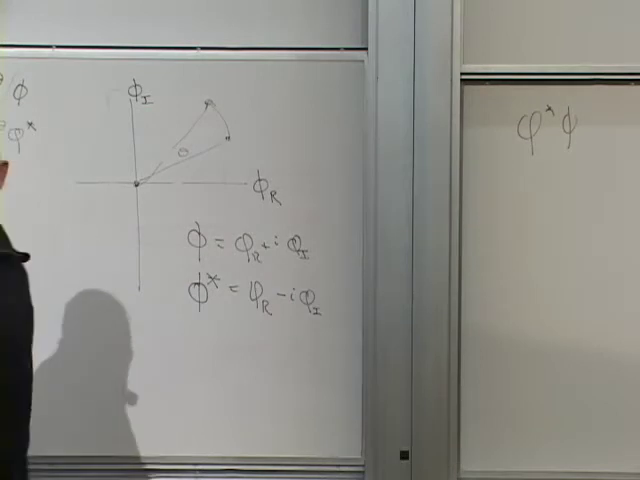
\includegraphics[width=0.80\textwidth]{lecture_07_figure_02.png}
\caption{\((\phi_R,\phi_I)\) 내부 평면 위의 복소장. 칠판에는 \(\phi\)과 \(\phi^*\)의 분해, 그리고 불변 반지름 \(\phi^*\phi\)이 기록되어 있다.}
\lectureframe{00:33:33}
\end{figure}

라그랑지안을 다음과 같이 두자.
\begin{equation}
  \mathcal L
  =\partial_\mu\phi^*\,\partial^\mu\phi
   -V(\phi^*\phi).
  \label{eq:l07-complex-lagrangian}
\end{equation}
복소장에는 관례적인 계수 \(1/2\)가 없다. 이 하나의 곱에 두 실수 성분의 운동항이 이미 모두 들어 있기 때문이다. 변환
\begin{equation}
  \phi'(x)=e^{i\theta}\phi(x),
  \qquad
  \phi^{*\prime}(x)=e^{-i\theta}\phi^*(x)
  \label{eq:l07-global-u1}
\end{equation}
은 모든 장의 값을 같은 각도만큼 회전시킨다. 여기서 \(\theta\)은 공간과 시간에 따라 변하지 않는 상수다. 프라임은 변환된 장을 나타내며, 미분을 뜻하지 않는다.

\(\theta\)이 상수이므로
\begin{equation}
  \partial_\mu\phi'=e^{i\theta}\partial_\mu\phi,
  \qquad
  \partial_\mu\phi^{*\prime}
  =e^{-i\theta}\partial_\mu\phi^*.
\end{equation}
위상 인자들이 운동항에서 서로 상쇄되고,
\(\phi^{*\prime}\phi'=\phi^*\phi\)도 성립한다. 따라서 \(\phi^*\phi\)에만 의존하는 퍼텐셜은 모두 같은 대칭성을 갖는다. \(\phi_R\)에만 의존하는 항은 내부 평면에서 한 방향을 택하게 하여 대칭성을 명시적으로 깨뜨린다.

\subsection{점 하나인 최소점과 원형 최소점}

대칭적인 퍼텐셜에는 정성적으로 다른 두 종류가 있다. 첫 번째는 원점에 유일한 최소점을 가지며, 예를 들면 다음과 같다.
\begin{equation}
  V_{\rm unbroken}=m^2\phi^*\phi,
  \qquad m^2>0.
\end{equation}
그래프는 회전 대칭인 포물면이다. 진공 \(\phi=0\)은 모든 회전에 대해 그대로이므로 대칭성이 깨지지 않는다.

이제 다음과 같이 택하자.
\begin{equation}
  V_{\rm broken}
  =-a\,\phi^*\phi+b(\phi^*\phi)^2,
  \qquad a,b>0.
  \label{eq:l07-mexican-hat}
\end{equation}
음의 이차항은 장을 원점에서 밀어내고, 양의 사차항은 장이 무한대로 발산하지 않게 한다. \(r^2=\phi^*\phi\)이라고 두고 최소화하면 다음을 얻는다.
\begin{equation}
  \frac{dV}{d(r^2)}=-a+2br^2=0,
  \qquad
  r^2=f^2=\frac{a}{2b}.
  \label{eq:l07-vacuum-radius}
\end{equation}
따라서 최소점들은 원을 이룬다. 퍼텐셜은 완벽한 회전 대칭을 유지하지만, 균일한 바닥 상태는 그 원 위의 한 점을 선택해야 한다.

\begin{figure}[htbp]
\centering
\includegraphics[width=0.72\textwidth]{lecture_07_figure_06.png}
\caption{회전면으로 그린 대칭성 깨짐 퍼텐셜. 원점은 불안정하고, 서로 축퇴된 최소점들은 원형 골짜기를 이룬다.}
\lectureframe{00:37:25}
\end{figure}

보통 공간의 각 점에 이 내부 평면의 작은 화살표 하나가 있다고 생각하자. 퍼텐셜은 화살표의 길이가 \(f\)이 되기를 요구한다. 기울기 에너지는 이웃한 화살표들이 거의 같은 방향을 향하도록 한다. 따라서 바닥 상태에서는 모든 곳의 각도가 같지만, 법칙은 어떤 각도도 선호하지 않는다. 이것이 연속 대칭성의 자발적 깨짐이다.

\section{영역 벽에서 매끄러운 비틀림으로}

경계 조건 실험을 다시 하자. 왼쪽 경계에서는 장을 진공점 \(A\)에 고정하고, 오른쪽 경계에서는 다른 진공점 \(B\)에 고정한다. 국소적으로 갑자기 뛰어 바뀌면 기울기가 커진다. 하지만 이산 대칭성의 경우와 달리, 장은 퍼텐셜의 최저점에 머문 채 원을 따라 연속적으로 변할 수 있다.

저에너지에서는 장을 \(\phi=f e^{i\alpha(x)}\)로 쓰자. 한 공간 차원에서 관련된 에너지는 다음과 같다.
\begin{equation}
  E[\alpha]
  =f^2\int_0^L dx\,\left(\frac{d\alpha}{dx}\right)^2.
  \label{eq:l07-angle-functional}
\end{equation}
양 끝의 각도를 고정하고 변분하면 다음을 얻는다.
\begin{equation}
  \frac{d^2\alpha}{dx^2}=0,
  \qquad
  \alpha(x)=\alpha_A+
    \frac{\alpha_B-\alpha_A}{L}\,x.
  \label{eq:l07-linear-twist}
\end{equation}
선호되는 배치는 시료 전체에 걸쳐 비틀림을 균일하게 퍼뜨린다. 그 에너지는 다음과 같이 스케일한다.
\begin{equation}
  E_{\rm twist}
  =f^2\frac{(\alpha_B-\alpha_A)^2}{L},
  \label{eq:l07-twist-energy}
\end{equation}
따라서 \(L\)을 늘리면 에너지를 임의로 작게 만들 수 있다.

\begin{figure}[htbp]
\centering
\begin{adjustbox}{max width=\linewidth}
\begin{tikzpicture}[x=0.95cm,y=0.95cm]
  \begin{scope}
    \draw[->] (0,0) -- (6.2,0) node[right] {$x$};
    \draw[->] (0,0) -- (0,3.5) node[above] {$\alpha(x)$};
    \draw[very thick,blue!70!black] (0.45,0.65) -- (5.7,2.85);
    \fill (0.45,0.65) circle (1.8pt) node[left] {$\alpha_A$};
    \fill (5.7,2.85) circle (1.8pt) node[right] {$\alpha_B$};
    \node at (3.1,-0.65) {physical space};
  \end{scope}
  \begin{scope}[xshift=9.2cm,yshift=1.65cm]
    \draw[thick] (0,0) circle (1.8);
    \fill (1.55,-0.92) circle (1.8pt) node[below right] {$A$};
    \fill (-0.45,1.74) circle (1.8pt) node[above] {$B$};
    \draw[very thick,blue!70!black,-{Latex[length=2.5mm]}]
      (1.55,-0.92) arc[start angle=-31,end angle=104,radius=1.8];
    \node at (0,-2.35) {vacuum circle};
  \end{scope}
\end{tikzpicture}
\end{adjustbox}
\caption{같은 저에너지 배치를 두 방식으로 나타냈다. 각도는 물리적 공간을 따라 선형적으로 변하고, 장은 내부 공간의 진공 원을 따라 짧은 호를 따른다.}
\end{figure}

\begin{classroomqa}
\audiencequestion{원을 따라가는 길이 두 가지일 수 있습니다. 장은 어느 길을 따르며, 더 긴 길에 갇힐 수도 있나요?
\lecturetimestamp{00:41:54}}
\lecturerresponse{일반적인 양 끝점에 대해서는 각도 변화가 더 짧은 경로가 기울기가 작으므로 에너지도 더 낮습니다. 서로 정반대인 양 끝점에서는 가장 간단한 두 경로의 에너지가 같습니다. 끝점 하나를 천천히 움직여 준비한 배치는 추가 감김수를 유지한 채 에너지 장벽 뒤에 갇힐 수 있습니다. 그러나 주어진 일반적인 양 끝점 쌍에 대해서는 비틀림이 없는 최단 경로가 바닥 상태입니다.}
\end{classroomqa}

\begin{classroomqa}
\audiencequestion{경로가 골짜기 바닥을 벗어나 내부를 가로질러 전체적으로 더 짧아질 수도 있나요?
\lecturetimestamp{00:43:32}}
\lecturerresponse{저에너지의 긴 시료에서는 반지름 방향 퍼텐셜을 올라가는 것이 유리하지 않다. 위의 변분법 계산에서 보았듯, 반지름을 진공값에 고정하고 각도를 선형적으로 변화시키는 것이 유효 에너지를 최소화한다. 특정 퍼텐셜을 가진 유한한 계에서는 반지름 방향 운동과 각도 운동을 함께 최소화할 수 있지만, 골드스톤 결론은 골짜기를 따라 부드럽게 움직이는 배치가 우세해지는 임의로 긴 파장의 극한에 관한 것이다.}
\end{classroomqa}

\begin{classroomqa}
\audiencequestion{원형 골짜기를 기울여 특정 각도를 더 낮게 만들면 무엇이 달라지나요?
\lecturetimestamp{00:44:33}}
\lecturerresponse{그러면 대칭성이 명시적으로 깨진다. 한 점이 참된 바닥 상태가 되고, 원을 따라 움직일 때 복원력이 생겨 각도 들뜸은 더 이상 정확히 질량이 없다.}
\end{classroomqa}

\section{영운동량 진동의 비용으로서의 질량}

매끄러운 비틀림은 에너지가 기울기에서만 비롯되는 장을 보여 준다. 이것이 왜 질량이 없는 입자를 뜻하는지 이해하려면 상대론적 분산 관계를 비교하자.
\begin{equation}
  \omega^2=\bm{k}^2+m^2.
  \label{eq:l07-dispersion}
\end{equation}
파동 \(e^{i(\bm{k}\cdot\bm{x}-\omega t)}\)은 운동량 \(\bm{k}\)을 갖는다. \(m=0\)이면 파장이 무한히 길어질수록 에너지는 0으로 다가간다.
\(\omega=|\bm{k}|\to0\). \(m\ne0\)이면 공간적으로 균일한 모드 \(\bm{k}=0\)도 각진동수 \(\omega=m\)로 계속 진동한다. 질량은 영운동량에서 남는 최소 에너지다.

이 구분은 라그랑지안에서도 드러난다. 항
\begin{equation}
  -\frac12m^2\varphi^2
\end{equation}
은 균일한 변위에도 복원력을 준다. 미분항만 있는 장에는 그런 복원력이 없다. 파장을 길게 만들수록 기울기 에너지는 0에 가까워진다.

\subsection{두 모드를 분리하는 극좌표}

대칭성이 깨진 복소장을 다음과 같이 쓰자.
\begin{equation}
  \phi(x)=\rho(x)e^{i\alpha(x)}.
  \label{eq:l07-polar}
\end{equation}
\(\rho\)와 \(\alpha\)은 모두 장이다. 미분하면 다음을 얻는다.
\begin{align}
  \partial_\mu\phi
  &=e^{i\alpha}
    \left(\partial_\mu\rho+i\rho\,\partial_\mu\alpha\right),\\
  \partial_\mu\phi^*
  &=e^{-i\alpha}
    \left(\partial_\mu\rho-i\rho\,\partial_\mu\alpha\right).
\end{align}
교차항이 상쇄되어 다음과 같이 남는다.
\begin{equation}
  \partial_\mu\phi^*\,\partial^\mu\phi
  =(\partial_\mu\rho)(\partial^\mu\rho)
   +\rho^2(\partial_\mu\alpha)(\partial^\mu\alpha).
  \label{eq:l07-polar-kinetic}
\end{equation}
\(\phi^*\phi=\rho^2\)이므로
\begin{equation}
  \mathcal L
  =(\partial\rho)^2+\rho^2(\partial\alpha)^2-V(\rho^2).
  \label{eq:l07-polar-lagrangian}
\end{equation}
퍼텐셜에는 \(\rho\)가 들어가지만 \(\alpha\)는 들어가지 않는다. 이 부재가 대칭성을 가장 유용한 형태로 보여 준다.

\begin{figure}[htbp]
\centering
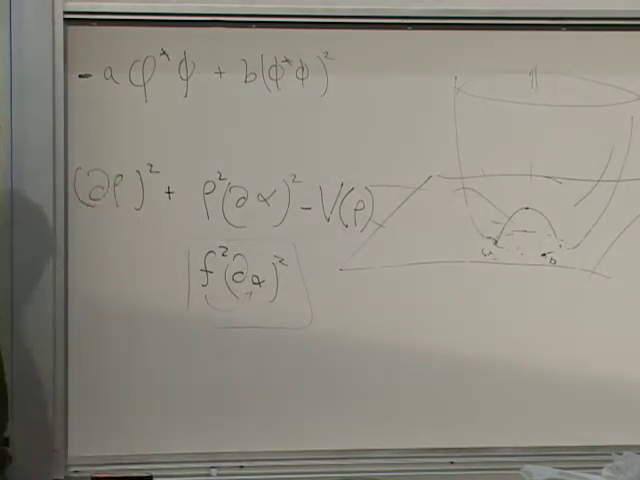
\includegraphics[width=0.88\textwidth]{lecture_07_figure_03.png}
\caption{극좌표 장의 라그랑지안, 상자로 표시한 저에너지 각도 항, 그리고 대칭성 깨짐 퍼텐셜. 반지름 방향 운동은 퍼텐셜을 거슬러 올라가고, 각도 방향 운동은 골짜기를 따른다.}
\lectureframe{00:56:40}
\end{figure}

매우 저에너지인 들뜸에서는 장이 \(\rho=f\)에 가깝게 유지된다. 그러면
\begin{equation}
  \mathcal L_{\rm angular}
  \simeq f^2(\partial_\mu\alpha)(\partial^\mu\alpha).
\end{equation}
계수 \(1/2\)에 관한 관례에 따라 정준 정규화된 각도 장을 다음과 같이 정의하자.
\begin{equation}
  \beta=\sqrt{2}\,f\alpha,
  \qquad
  \mathcal L_{\rm angular}
  =\frac12(\partial_\mu\beta)(\partial^\mu\beta).
  \label{eq:l07-goldstone-field}
\end{equation}
\(\beta^2\) 항은 없다. 이 각도 장의 양자는 질량이 없다. 이들이 골드스톤 보손이다.

반지름 방향 장의 거동은 다르다. \(\rho\)을 \(f\)에서 한꺼번에 변위시키면 골짜기로 되돌아가다가 지나쳐 진동한다. \(\rho=f+h\)이면 식~\eqref{eq:l07-mexican-hat}을 전개하여 다음을 얻는다.
\begin{equation}
  V(f+h)=V(f)+\frac12m_h^2h^2+\cdots,
\end{equation}
따라서 \(h\)에는 질량이 있다. 기하학적으로 각도 방향은 평평하고 반지름 방향은 굽어 있다.

\begin{classroomqa}
\audiencequestion{장이 방사 방향으로 변위되면 단순히 다시 아래로 떨어지는가? 그다음에는 무슨 일이 일어나는가?\lecturetimestamp{00:57:10}}
\lecturerresponse{각운동이 없으면 장은 최소점 쪽으로 떨어졌다가 그 지점을 지나쳐 방사 방향으로 진동한다. 공간적으로 균일한 진동은 공간 운동량이 없지만 주파수는 0이 아니며, 그 주파수가 방사 방향 여기의 질량이다. 이와 달리 공간적으로 균일한 각방향 변위는 다른 진공 상태에 도달하며, 복원력은 없다.}
\end{classroomqa}

이 예에서 골드스톤 원리의 내용은 다음과 같다. 연속 전역 대칭성이 자발적으로 깨지면 진공 다양체의 서로 독립적인 평탄 방향마다 질량이 없는 모드가 하나씩 생긴다.
\editorialnote{이 진술은 상대론적 장 이론의 통상적인 조건을 가정한다. 비상대론적 다체계에서는 난부--골드스톤 모드의 개수와 분산 관계가 더 미묘할 수 있지만, 이 상대론적 \(U(1)\) 모형에서는 강의의 장파장 결론이 여전히 옳다.}

\section{스핀파, 줄, 그리고 소리}

정리는 추상적이지만, 그 작동 원리는 익숙하다. 등방성 강자성체에서는 모든 스핀을 함께 회전시켜도 에너지가 변하지 않는다. 시료 전반에 걸쳐 방향이 아주 천천히 변하도록 하면 스핀파를 얻는다. 그 에너지 비용은 파수가 작아질수록 사라지므로, 이 스핀파는 깨진 스핀 회전 대칭성의 골드스톤 모드다.

긴 탄성 줄도 또 하나의 그림을 제공한다. 중력을 무시하고 줄 전체를 수직으로 옮길 수 있도록 양 끝을 고정하자. 줄 전체의 균일한 수직 이동에는 에너지가 들지 않는다. 줄을 따라 이동량이 천천히 변하게 하면 장파장 횡파가 된다. 균일한 대칭 연산이 부드럽고 위치에 따라 달라지는 변형으로 확장된 것이다.

\begin{figure}[htbp]
\centering
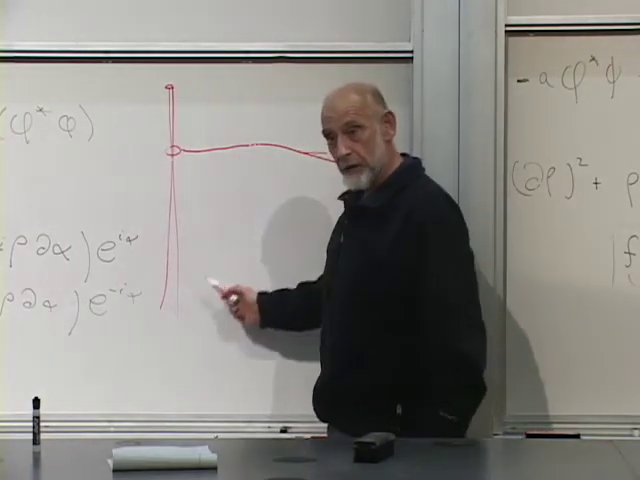
\includegraphics[width=0.68\textwidth]{lecture_07_figure_04.png}
\caption{골드스톤 모드의 비유를 위해 그린, 천천히 변하는 줄의 형상. 물리적으로 중요한 것은 장파장 변형의 작은 기울기이지 곡선의 수직 위치가 아니다.}
\lectureframe{01:04:19}
\end{figure}

\begin{classroomqa}
\audiencequestion{줄이 운동량은 0이면서 진동 에너지를 가질 수 있나요?
\lecturetimestamp{01:04:41}}
\lecturerresponse{수직 방향의 역학적 운동량과 줄을 따라 전달되는 파동의 운동량을 구별해야 한다. 정상파는 \(+k\)과 \(-k\)을 갖는 모드들의 중첩이어서 순운동량이 0일 수 있지만, 그래도 에너지를 전달한다. 장 이론의 비유에서 운동량은 축을 따라가는 파수를 뜻하고, 수직 변위는 내부 장 좌표를 나타낸다.}
\end{classroomqa}

슬링키는 종파의 비유를 제공한다. 이상화한 무한 슬링키를 축을 따라 통째로 옮겨도 아무것도 변하지 않는다. 이웃한 부분들을 조금씩 다른 거리만큼 옮기면 부드러운 압축파가 생긴다. 고체나 유체에서도 장파장 소리는 이와 비슷하게 집단 변위와 밀도 변화에서 비롯된다. 스핀파, 횡방향 줄파, 소리는 미시적으로 같은 들뜸은 아니지만 결정적인 양상은 공유한다. 균일한 연속 연산에는 에너지가 들지 않고, 그것이 천천히 변하는 형태로 나타나면 연성 모드가 된다.
\editorialnote{결정에서는 음향 포논을 자발적으로 깨진 연속 병진 대칭성의 난부--골드스톤 모드로 기술하는 것이 일반적이다. 줄과 슬링키는 같은 미분항만으로 이루어진 에너지 구조를 드러내기 위해 강의에서 사용한 역학적 비유다.}

이 용어는 짧은 강의실 농담을 할 만큼 중요하다. 이들은 제프리 골드스톤의 이름을 딴 \emph{골드스톤} 보손이지, 게이지 보손이 아니다. 강의에서는 골드스톤이 서스킨드의 친구였다고 언급한 뒤, 이와 실제로 다른 주제인 게이지 불변성으로 넘어간다.

\section{전역 위상 대칭성에서 게이지 대칭성으로}

\(U(1)\) 위상 대칭성은 전하 보존과 관련된 대칭성으로 이미 강의에서 다룬 바 있다. 하전 입자 장은 복소수이며, 이런 장에 공통 위상 인자를 곱해도 전역 이론은 변하지 않는다. 직관을 위해 전기적 전하라고 말할 수 있지만, 그 전하는 다른 \(U(1)\) 양자수일 수도 있다. 실제 광자는 질량이 없다. 궁극적으로 살펴볼 대상은 질량이 있는 \(Z\) 같은 광자형 장이다.

새로운 질문은 다음 변환이
\begin{equation}
  \phi'(x)=e^{i\theta(x)}\phi(x)
  \label{eq:l07-local-u1}
\end{equation}
\(\theta\)이 시공간에 걸쳐 임의로 변해도 대칭성이 될 수 있는가이다. 함수 \(\theta(x)\)는 변환 매개변수이지, 추가적인 동역학적 장이 아니다. 이 제안을 미분하여 확인해 보자.
\begin{equation}
  \partial_\mu\phi'
  =e^{i\theta}
   \left[\partial_\mu\phi+i(\partial_\mu\theta)\phi\right].
  \label{eq:l07-local-derivative}
\end{equation}
상수 \(\theta\)일 때는 추가 항이 없었다. 켤레장에 대해서는
\begin{equation}
  \partial_\mu\phi^{*\prime}
  =e^{-i\theta}
   \left[\partial_\mu\phi^*-i(\partial_\mu\theta)\phi^*\right].
\end{equation}
을 얻는다. 두 식의 곱은
\begin{align}
  \partial_\mu\phi^{*\prime}\partial^\mu\phi'
  ={}&
  \partial_\mu\phi^*\partial^\mu\phi
  i\left(
      \phi\,\partial_\mu\phi^*
      -\phi^*\partial_\mu\phi
    \right)\partial^\mu\theta
  \nonumber\\
  &+\phi^*\phi\,
    \partial_\mu\theta\,\partial^\mu\theta.
  \label{eq:l07-local-failure}
\end{align}
이다. \(\phi^*\phi\)는 불변이므로 퍼텐셜은 여전히 불변이지만, 보통의 운동항은 불변이 아니다. 전역 대칭성이 저절로 국소 대칭성이 되는 것은 아니다.

\begin{classroomqa}
\audiencequestion{멕시코 모자 그림에서 이런 실패는 원형 골짜기 주변에 굴곡이 있다는 뜻인가요?
\lecturetimestamp{01:19:37}}
\lecturerresponse{아닙니다. 퍼텐셜은 각도 방향으로 완벽히 평평할 수 있습니다. 위상이 시공간의 점마다 달라질 때 기울기 때문에 비용이 생기는 것입니다. 이는 골짜기가 울퉁불퉁해진다는 뜻이 아니라 보통의 미분항이 공간적 변화를 감지한다는 뜻입니다.}
\end{classroomqa}

\subsection{상쇄 역할을 하는 벡터장}

자연에 존재하는 광자, \(W\), \(Z\) 및 글루온의 상호작용은 강체 변환만이 아니라 국소 게이지 대칭성으로 구성된다. 국소 위상 변환을 대칭성으로 만들려면 사벡터 장 \(A_\mu\)을 이론에 추가해야 한다. 전자기학에서 \(A_0\)은 스칼라 퍼텐셜이며, 세 공간 성분은 벡터 퍼텐셜을 이룬다. 이들의 미분으로 전기장과 자기장을 구성한다.

내부적으로 일관된 다음 관례를 택하자.
\begin{equation}
  \phi'=e^{i\theta}\phi,
  \qquad
  A'_\mu=A_\mu-\partial_\mu\theta,
  \qquad
  D_\mu=\partial_\mu+iA_\mu.
  \label{eq:l07-gauge-convention}
\end{equation}
상쇄를 확인하는 과정에서 칠판의 부호 하나가 바뀌지만, 식 \eqref{eq:l07-gauge-convention}은 세 부호를 함께 정한다. 게이지 결합 상수와 전하는 일단 \(A_\mu\)에 흡수했다.
\editorialnote{\(q\)와 결합 상수 \(g\)를 명시하면 다음과 같이 쓸 수 있다.
\(D_\mu=\partial_\mu+igqA_\mu\) 및
\(A'_\mu=A_\mu-(gq)^{-1}\partial_\mu\theta\). 강의에서는 상쇄가 잘 드러나도록 이 상수들을 생략했다.}

켤레장에 대해서는
\begin{equation}
  D_\mu\phi^*=\partial_\mu\phi^*-iA_\mu\phi^*.
\end{equation}
을 얻는다. 이제
\begin{align}
  D'_\mu\phi'
  &=
  \left(\partial_\mu+iA'_\mu\right)e^{i\theta}\phi
  \nonumber\\
  &=
  e^{i\theta}
  \left[
    \partial_\mu\phi+i(\partial_\mu\theta)\phi
    +i(A_\mu-\partial_\mu\theta)\phi
  \right]
  \nonumber\\
  &=e^{i\theta}D_\mu\phi.
  \label{eq:l07-covariant-transform}
\end{align}
이다. \(\theta\)의 원치 않는 미분항은 \(A_\mu\)의 변환으로 상쇄된다. 마찬가지로
\begin{equation}
  D'_\mu\phi^{*\prime}=e^{-i\theta}D_\mu\phi^*.
\end{equation}
이고, 두 식의 곱은 불변이다. \emph{공변} 미분이라는 말은 미분한 양이 장 자체와 같은 간단한 방식으로 변환한다는 뜻이다.

\section{게이지 장의 동역학}

미분항을 고치기 위해 \(A_\mu\)만 도입하면 그 자체의 동역학이 없게 된다. 게이지 불변인 장세기는 다음과 같다.
\begin{equation}
  F_{\mu\nu}
  =\partial_\mu A_\nu-\partial_\nu A_\mu.
  \label{eq:l07-field-strength}
\end{equation}
장세기는 반대칭이므로 \(F_{\mu\mu}=0\)이다. 시간--공간 성분에는 전기장이 들어 있고, 공간--공간 성분에는 자기장이 들어 있다. 익숙한 3차원 벡터 표현에서 전자기장 에너지 밀도는 \(\bm E^2+\bm B^2\)에 비례하고, 로런츠 라그랑지안은 \(\bm E^2-\bm B^2\)에 비례한다. 부호는 계량 관례에 따라 달라진다.

\begin{classroomqa}
\audiencequestion{전자기장의 에너지와 라그랑지안은 무엇인가요?
\lecturetimestamp{01:33:20}}
\lecturerresponse{에너지는 \(E^2+B^2\)로 이루어지고, 라그랑지안에는 \(E^2-B^2\)이 쓰인다. 공변적으로는 후자를 \(F_{\mu\nu}F^{\mu\nu}\)의 관례적인 상수배로 쓴다. 반대칭 텐서는 벡터 퍼텐셜의 4차원 컬이다.}
\end{classroomqa}

장세기 자체는 게이지 불변이다.
\begin{align}
  F'_{\mu\nu}
  &=
  \partial_\mu(A_\nu-\partial_\nu\theta)
  -\partial_\nu(A_\mu-\partial_\mu\theta)
  \nonumber\\
  &=
  F_{\mu\nu}
  -\partial_\mu\partial_\nu\theta
  +\partial_\nu\partial_\mu\theta
  =F_{\mu\nu}.
  \label{eq:l07-field-strength-invariant}
\end{align}
마지막 등식은 보통의 혼합 편미분이 서로 교환된다는 사실에서 따른다. 따라서 표준적인 게이지 불변 라그랑지안은 다음과 같다.
\begin{equation}
  \boxed{
  \mathcal L
  =(D_\mu\phi)^*D^\mu\phi
  -V(\phi^*\phi)
  -\frac14F_{\mu\nu}F^{\mu\nu}}
  \label{eq:l07-scalar-qed}
\end{equation}
계량에 대해 선택한 부호와 정규화 관례는 별도로 두었다.

\begin{figure}[htbp]
\centering
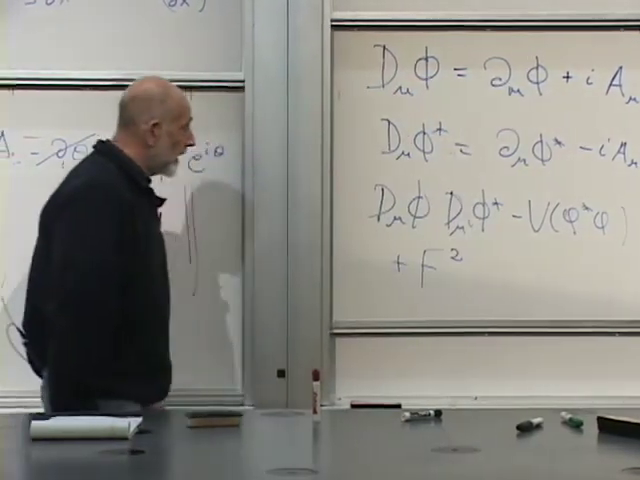
\includegraphics[width=0.84\textwidth]{lecture_07_figure_05.png}
\caption{칠판에 적힌 공변 미분과 조립된 게이지 불변 라그랑지안. 변환 구조가 잘 드러나도록 수치 계수는 생략했다.}
\lectureframe{01:38:45}
\end{figure}

이 구성은 전역 \(U(1)\) 대칭성을 국소 대칭성으로 확장하지만, 그 대가------로 새로운 벡터장을 도입한다. 아벨 예에서 그 장은 전자기 퍼텐셜이다.

\begin{classroomqa}
\audiencequestion{처음의 라그랑지안에는 보통의 미분이 쓰였습니다. 이를 공변 미분으로 바꾸고 그 결과를 실제 이론이라고 불러도 되는 이유가 무엇인가요?
\lecturetimestamp{01:42:55}}
\lecturerresponse{우리는 새로운 확장 이론, 즉 하전 물질과 게이지 장으로 이루어진 이론을 구성하는 중이다. 국소 게이지 불변성이 두 요소의 결합을 결정한다. 그렇게 얻은 양자 이론은 수학적으로 일관된 구조이며, 자연이 광자와 약한 게이지 장을 구성하는 방식과 일치한다. 상대론적 벡터 장을 일관성 없이 결합하면 비물리적 편극이나 확률 보존 위반이 생길 수 있다. 따라서 게이지 원리는 기존 자유 스칼라 이론을 겉으로만 바꿔 쓴 것이 아니다.}
\end{classroomqa}

\begin{classroomqa}
\audiencequestion{새로운 장을 더하는 것이 수정의 핵심적인 정당화 근거인가요?\lecturetimestamp{01:44:57}}
\lecturerresponse{그렇습니다. \(A_\mu\)가 없으면 국소적으로 회전한 장의 미분에 상쇄되지 않은 \(\partial_\mu\theta\)가 남습니다. \(A_\mu\)와 그 변환 법칙을 도입하면 이 항들이 상쇄됩니다. 기하학의 언어로는 \(A_\mu\)가 다발 위의 접속입니다. 이보다 깊은 수학은 실제로 유용하지만, 여기서는 위의 대수적 전개에 필요한 내용이 모두 담겨 있습니다.}
\end{classroomqa}

\section{게이지 보손에 질량항을 직접 넣을 수 없는 이유}

일반적인 보손 장의 질량은 이차항으로 나타냅니다. 다음 항을 더하고 싶을 수 있습니다.
\begin{equation}
  \Delta\mathcal L_{\rm Proca}
  =\frac12m^2A_\mu A^\mu.
  \label{eq:l07-proca}
\end{equation}
\(A_\mu\mapsto A_\mu-\partial_\mu\theta\) 아래에서,
\begin{equation}
  A'_\mu A^{\mu\prime}
  =
  A_\mu A^\mu
  -2A^\mu\partial_\mu\theta
  +\partial_\mu\theta\,\partial^\mu\theta,
\end{equation}
따라서 식~\eqref{eq:l07-proca}은 게이지 불변이 아닙니다. 국소 대칭성을 유지하면서 이 게이지 이론에 질량을 임의로 넣을 수는 없습니다.

\begin{figure}[htbp]
\centering
\includegraphics[width=0.72\textwidth]{lecture_07_figure_07.png}
\caption{제안된 벡터 보손의 질량항
\(\tfrac12m^2A_\mu A^\mu\)은 \(A_\mu\mapsto A_\mu-\partial_\mu\theta\) 아래에서 불변이 아닙니다. 이 실패가 힉스 메커니즘으로 이어지는 장애물입니다.}
\lectureframe{01:39:48}
\end{figure}

이것이 겉보기에 막다른 상황입니다. 게이지 불변성은 광자가 질량이 없는 이유를 설명하고, 비물리적 자유도가 이론에 들어오는 것을 막아 주지만, \(W\)와 \(Z\)는 질량이 있습니다. 이 난관을 벗어나기 위해 벡터 질량을 명시적으로 넣을 수는 없습니다. 게이지 불변 라그랑지안에 이미 들어 있는 장들에서 해법이 나와야 합니다.

\begin{classroomqa}
\audiencequestion{게이지 불변성을 도입하는 것 자체가 골드스톤 보손을 만들어 내나요?\lecturetimestamp{01:45:51}}
\lecturerresponse{아닙니다. 골드스톤 보손은 벡터 퍼텐셜을 도입하기 전에 연속적인 \emph{전역} 대칭성이 자발적으로 깨지면서 생겼습니다. 대칭성이 국소 대칭성이 되면, 위상이 위치에 따라 변하더라도 \(A_\mu\)를 통해 그 변화를 상쇄할 수 있습니다. 대칭성이 깨진 게이지 이론에서는 각도 모드가 더 이상 독립적인 질량 없는 입자가 아닙니다. 그 모드는 이제 질량을 갖게 된 벡터 장의 추가 편극을 제공합니다. 다음 강의에서는 이 내용을 단순히 선언하는 데 그치지 않고 유도하겠습니다.}
\end{classroomqa}

\begin{classroomqa}
\audiencequestion{이 내용은 강이 굽이쳐 흐르는 이유도 설명하나요?\lecturetimestamp{01:47:03}}
\lecturerresponse{여기서는 직접적인 연관성이 알려져 있지 않습니다. 유체의 소용돌이와 생물의 형태도 대칭성 방법으로 기술할 수는 있습니다. 장론의 발상이 뜻밖의 곳에서 발견되더라도 놀랄 일은 아니지만, 이 강의는 강의 굽이침을 설명하는 게이지 이론을 제시하지 않습니다.}
\end{classroomqa}

\section{강의의 마무리}

이제 처음에 약속한 두 가지 요소를 갖추었습니다. 진공 상태들이 원을 이루는 연속적인 전역 대칭성에는 평평한 각도 방향이 있고, 그 방향의 느린 변화는 질량 없는 골드스톤 장이 됩니다. 국소 대칭성에는 게이지 접속과 공변미분이 필요하며, 식~\eqref{eq:l07-proca}에 나타난 직접적인 벡터 질량항은 허용되지 않습니다.

다음 단계에서는 식~\eqref{eq:l07-mexican-hat}의 대칭성이 깨진 퍼텐셜을 식~\eqref{eq:l07-scalar-qed}의 게이지 불변 이론에 넣겠습니다. 그러면 두 가지 일이 함께 일어납니다. 골드스톤 입자는 물리적 스펙트럼에서 사라지고, 벡터 장은 질량을 얻습니다. 통상적인 교육용 표현으로는 게이지 대칭성이 자발적으로 깨진다고 합니다. 더 정확히 말하면 게이지 중복성은 그대로 유지되고, 이론은 질량을 가진 벡터 들뜸이 존재하는 힉스 상에 놓입니다.
\editorialnote{국소 게이지 대칭성은 서로 다른 관측 가능한 상태 사이에서 작용하는 일반적인 물리적 대칭성이 아니라 기술상의 중복성입니다. 이 강의에서는 게이지 대칭성의 자발적 깨짐이라는 표준적인 약칭을 사용합니다. 게이지 불변인 물리적 진술은 힉스 상에서 자유도의 배열이 재편된다는 것입니다.}

이것이 힉스 현상입니다. 아직 이 현상을 직접 살펴보지는 않았습니다. 이번 강의에서는 문제를 충분히 정확하게 정식화하는, 꼭 필요하지만 더 어려운 작업을 했습니다. 그래서 해법이 제시되면 피할 수 없는 결론이 될 것입니다.
\chapter{힉스 메커니즘: 게이지 보손은 어떻게 질량을 얻는가}

이제 앞선 강의에서 다룬 두 가지 생각을 결합해 보자. 전역 \(U(1)\) 대칭성이 깨진 복소 스칼라장에는 질량이 있는 방사 방향 진동과 질량이 없는 각방향 진동이 있다. 국소적으로 불변인 \(U(1)\) 이론에는 질량이 없는 게이지장이 있다. 스칼라장이 전하를 띠고 평형 크기가 영이 아니면, 이 두 진술을 단순히 더할 수는 없다. 각방향 모드와 게이지장이 결합하면 게이지장이 질량을 얻고, 겉보기의 골드스톤 보손은 독립적인 입자가 아니게 되며, 방사 방향 힉스 모드는 남는다.

광자를 모형 게이지 보손으로 삼겠지만, 물리적 결론의 대상으로 삼지는 않는다. 진공에서는 전자기 \(U(1)\)가 깨지지 않으므로 실제 광자는 질량이 없다. 게이지 군과 스칼라 다중항이 더 복잡한 전약 이론에서는 같은 메커니즘이 \(W^\pm\)와 \(Z\)에 작용한다. 아벨 모형은 군론으로 메커니즘을 가리지 않고 드러내 준다.

\begin{classroomqa}\audiencequestion{앞서 한 논의는 힉스 메커니즘이 실제 광자에 질량을 준다는 뜻이었나요?\lecturetimestamp{00:00:23}}\lecturerresponse{아닙니다. 광자와 관련된 \(U(1)\)가 깨진 상에 있다면 \emph{어떻게 될지} 묻는 것입니다. 그런 가상의 광자는 질량을 얻게 됩니다. 실제 전자기 진공은 그런 상에 있지 않습니다. 입자물리학에서 이 메커니즘은 대신 \(W\)와 \(Z\)의 질량을 설명합니다.}\end{classroomqa}

전하 보존과 관련된 대칭은 위상 회전입니다.
\begin{equation}
  \phi(x)\longmapsto e^{i\theta}\phi(x),
\end{equation}
이는 \(U(1)\)라 불리는 내부 회전이다. 초전도체는 깨진 상의 실제 유사 사례다. 초전도체 내부에서는 전자기장이 유한한 침투 깊이를 가지며, 중요한 여러 측면에서 질량이 있는 장처럼 거동한다. 초전도체 바깥에서는 익숙한 질량 없는 광자가 다시 나타난다.

\section{장에 대한 질량의 의미}

\subsection{분산 관계와 영운동량 에너지 간극}

힉스장을 도입하기 전에 질량이 정확히 무엇을 뜻하는지 정해 두는 편이 좋다. 파동에서는
\begin{equation}
  E=\hbar\omega,
  \qquad
  p=\hbar k,
  \label{eq:l08-quantum-wave}
\end{equation}
따라서 \((E,p)\) 그래프와 \((\omega,k)\) 그래프는 \(\hbar\) 계수만큼의 차이를 제외하면 같은 정보를 담는다. 빈 공간에서 질량 없는 상대론적 여기 상태는 다음을 만족한다.
\begin{equation}
  E=c|p|,
  \qquad
  \omega=c|k|.
  \label{eq:l08-massless-dispersion}
\end{equation}
\(k\)의 두 부호는 서로 반대인 전파 방향을 구분한다. 핵심은 \(\omega\)가 \(k\)와 함께 0으로 간다는 점이다.

질량이 있는 상대론적 입자는 다음 관계를 따른다.
\begin{equation}
  E^2=c^2p^2+m^2c^4.
  \label{eq:l08-massive-dispersion}
\end{equation}
단위계 \(c=\hbar=1\)에서는
\begin{equation}
  \omega^2=k^2+m^2.
\end{equation}
\(k=0\)에서 에너지는 \(E=mc^2\)이며, 자연 단위계에서는 간단히 \(m\)이다.
따라서 질량은 운동량이 영인 모드의 영이 아닌 에너지 간극이다.

\begin{figure}[htbp]
\centering
\begin{adjustbox}{max width=\linewidth}
\begin{tikzpicture}[x=1.05cm,y=1.05cm]
  \begin{scope}
    \draw[->] (-0.2,0) -- (4.2,0) node[right] {\(k\)};
    \draw[->] (0,-0.2) -- (0,3.1) node[above] {\(\omega\)};
    \draw[very thick,blue!65!black] (0,0) -- (3.8,2.75);
    \draw[very thick,orange!70!black] (0,0) -- (3.8,1.75);
    \node[blue!65!black,rotate=36] at (2.65,2.15)
      {\(\omega=c_{\rm vac}k\)};
    \node[orange!70!black,rotate=24] at (2.65,1.05)
      {ordinary medium};
    \node[below] at (2,-0.45) {gapless};
  \end{scope}
  \begin{scope}[xshift=6.2cm]
    \draw[->] (-0.2,0) -- (4.2,0) node[right] {\(k\)};
    \draw[->] (0,-0.2) -- (0,3.1) node[above] {\(\omega\)};
    \draw[very thick,domain=0:3.8,samples=120,smooth,teal!70!black]
      plot (\x,{sqrt(0.9+0.45*\x*\x)});
    \draw[dashed] (0,0.95) -- (1.0,0.95);
    \node[left] at (0,0.95) {\(m\)};
    \node[teal!70!black] at (2.55,2.15)
      {\(\omega^2=k^2+m^2\)};
    \node[below] at (2,-0.45) {gapped};
  \end{scope}
\end{tikzpicture}
\end{adjustbox}
\caption{전파 속도가 달라지면 간극이 없는 분산 관계의 기울기가 달라진다. 여기에 질량을 부여하면 \(k=0\)에서 영이 아닌 간극이 생긴다.}
\label{fig:l08-dispersion}
\end{figure}

일반적인 투명 물질은 파동의 위상 속도를 낮출 수 있지만, 이 상대론적 질량 간극을 만들지는 않는다. 경계면에서는 입사파의 진동수가 고정되고 파수는 매질의 분산 관계에 맞춰 조정된다. 기울기를 바꾸는 것은 절편을 올리는 것과 같지 않다.
\editorialnote{물질에는 여러 전자기 분지가 있을 수 있으며, 플라스마나 공명 매질에는 영이 아닌 플라스마 주파수 간극이 있을 수 있다. 강의에서 비교하는 것은 일반적인 굴절 분지와 초전도 응답이다. 더 일반적으로 간극이 없다는 것은 \(\omega(k)\to0\)이며, 이 극한은 \(k\to0\)에서 취한다. 모든 비상대론적 매질에서 분산 관계가 정확히 선형일 필요는 없다.}

\begin{classroomqa}\audiencequestion{프리즘을 통과하는 경우처럼, 광자는 물질 속을 지나갈 때마다 질량을 얻나요?\lecturetimestamp{00:03:02}}\lecturerresponse{아닙니다. 굴절은 진동수와 파수의 관계를 바꾸어 전파 속도를 바꿀 수 있지만, 분산 가지는 여전히 \(k=0\)에서 \(\omega=0\)을 지난다. 반면 초전도상에서는 전자기 응답의 역침투 길이가 유한해지며, 이것이 질량의 유사량에 해당한다.}\end{classroomqa}

\begin{classroomqa}\audiencequestion{일정한 진동수의 빛이 유리에 들어가면 파수가 바뀌나요?\lecturetimestamp{00:09:20}}\lecturerresponse{그렇습니다. 정지한 경계면에서 시간 병진 대칭이 보존되므로 진동수는 고정된다. 유리에서는 분산 곡선의 기울기가 다르므로 같은 \(\omega\)에 대응하는 \(k\)가 달라지고, 따라서 파장도 달라진다.}\end{classroomqa}

기울기
\begin{equation}
  v_g=\frac{d\omega}{dk}
\end{equation}
는 파동 묶음의 군속도다. 이 기울기가 \(k\)에 따라 달라지면 푸리에 성분마다 속도가 달라져 파동 묶음이 분산한다. 그래서 \(\omega(k)\)라는 관계를 \emph{분산 관계}라고 부른다.

\begin{classroomqa}\audiencequestion{이 곡선의 이름은 무엇이며, 기울기는 무엇을 나타내나요?\lecturetimestamp{00:11:02}}\lecturerresponse{이 곡선은 분산 관계다. 곡선의 도함수 \(d\omega/dk\)는 군속도다. 기울기가 일정하면 모든 파장이 같은 속도를 가지지만, 기울기가 변하면 파동 묶음이 퍼진다. 여기서 결정적인 구분은 곡선이 원점을 지나는지, 아니면 간극이 있는지다.}\end{classroomqa}

\subsection{균일한 진동은 정지한 입자다}

모드 \(k=0\)의 파장은 무한대다. 장은 모든 곳에서 같은 크기만큼 변위한다. 균일하게 변위시킨 뒤 놓아 보자. 장이 영이 아닌 진동수로 진동한다면 이에 대응하는 양자는 영이 아닌 정지 에너지를 가지므로 질량이 있다. 그 방향으로 복원력이 없다면 진동수는 영이 되고 모드는 질량이 없다.

이 진술은 고전적인 내용이다. 공간적으로 떨어진 입자들이 양자 중첩 상태에 있어야 하는 것은 아니다. 균일한 고전 장 배치는 단지 공간 전체에 동일한 장의 값이 놓인 상태다.

\begin{classroomqa}\audiencequestion{장 전체를 함께 이동시키는 것이 양자 얽힘과 같은 것인가요?\lecturetimestamp{00:10:04}}\lecturerresponse{아닙니다. 균일한 고전 장은 하나의 고전적 배치다. 얽힘은 위--아래와 아래--위 스핀 배치처럼 서로 다른 양자적 대안들 사이의 상관관계다. 여러 지점에 같은 장의 값을 준비하는 것 자체는 얽힘이 아니며, 순간적인 인과 반응을 뜻하지도 않는다.}\end{classroomqa}

정규화가 표준인 실수장에 대해
\begin{equation}
  \mathcal L
  =\frac12\partial_\mu\varphi\,\partial^\mu\varphi-V(\varphi),
\end{equation}
평형점 \(\varphi_0\)을 중심으로 전개하면
\begin{equation}
  V(\varphi_0+\eta)
  =V(\varphi_0)
   +\frac12V''(\varphi_0)\eta^2+\cdots.
\end{equation}
최솟값에서는 선형항이 사라지고, 장 방정식은 다음을 준다.
\begin{equation}
  \omega^2=\bm{k}^2+m^2,
  \qquad
  m^2=V''(\varphi_0).
  \label{eq:l08-curvature-mass}
\end{equation}
따라서 질량은 운동 방향에서 퍼텐셜의 곡률이다. 평평한 방향의 곡률은 0이므로 질량 없는 모드가 생긴다.

\section{깨진 복소 스칼라}

\subsection{방사 방향 운동과 각방향 운동}

복소 스칼라를 직교 좌표와 극좌표로 쓰면 다음과 같다.
\begin{equation}
  \phi=\phi_R+i\phi_I=\rho e^{i\alpha},
  \qquad
  \phi^*=\phi_R-i\phi_I=\rho e^{-i\alpha}.
  \label{eq:l08-polar-field}
\end{equation}
복소 평면은 \emph{내부} 장 공간이다. 물리적 시공간의 각 점 \(x\)에서 쌍
\((\phi_R(x),\phi_I(x))\)
은 그 내부 평면의 한 점을 지정한다. 내부 좌표축 중 어느 것도 실험실의 방향을 나타내지 않는다.

\begin{figure}[htbp]\centering
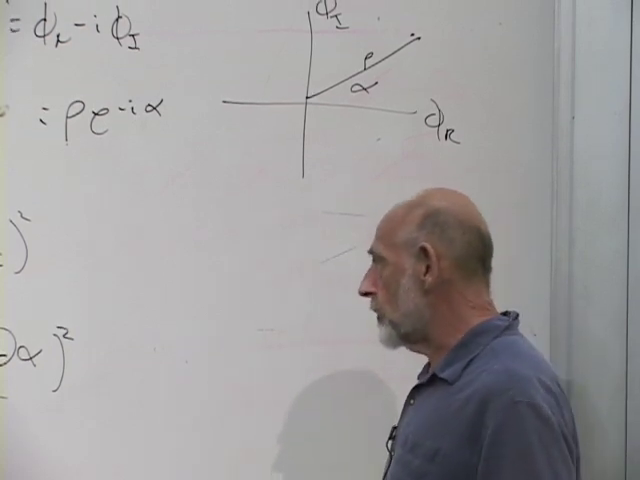
\includegraphics[width=0.72\textwidth]{lecture_08_figure_02.png}\caption{내부 \((\phi_R,\phi_I)\) 평면에 나타낸 복소 스칼라. 반지름은 \(\rho\)이고 \(\alpha\)는 내부 위상이다.}\lectureframe{00:24:41}\label{fig:l08-internal-plane}\end{figure}

스칼라 운동항은 다음과 같이 된다.
\begin{align}
  \partial_\mu\phi^*\,\partial^\mu\phi
  &=
  \partial_\mu\phi_R\,\partial^\mu\phi_R
  +\partial_\mu\phi_I\,\partial^\mu\phi_I
  \notag\\
  &=
  \partial_\mu\rho\,\partial^\mu\rho
  +\rho^2\partial_\mu\alpha\,\partial^\mu\alpha.
  \label{eq:l08-polar-kinetic}
\end{align}
전역적으로 \(U(1)\) 불변인 퍼텐셜은 \(\phi^*\phi=\rho^2\)에 의존하고 \(\alpha\)에는 의존하지 않는다. 예를 들면
\begin{equation}
  V(\phi)
  =\lambda\left(\phi^*\phi-\frac{f^2}{2}\right)^2,
  \qquad \lambda>0.
  \label{eq:l08-mexican-hat}
\end{equation}
최솟값들은 원을 이룬다. 물리 법칙은 공통 위상 회전에 대해 불변이지만, 평형 위상 하나를 택하면 그 원 위의 한 점이 선택된다.

\begin{figure}[htbp]\centering
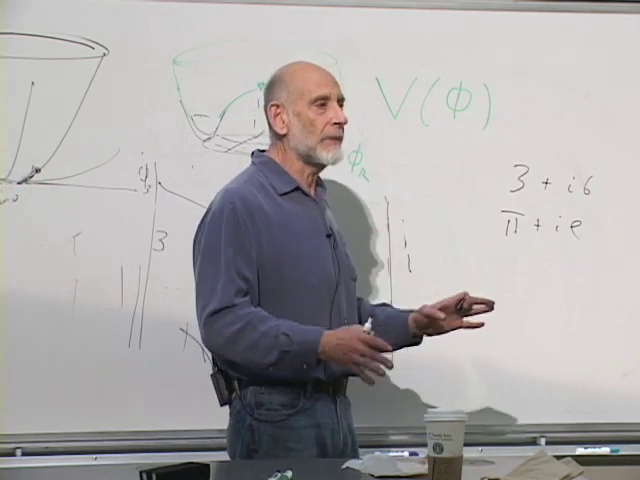
\includegraphics[width=0.78\textwidth]{lecture_08_figure_03.png}\caption{칠판에 그린 방사 방향 퍼텐셜 스케치. 장의 값이 원점에 있지 않더라도 퍼텐셜은 내부 장 값의 회전에 대해 대칭이다.}\lectureframe{00:34:22}\label{fig:l08-radial-potential-board}\end{figure}

\begin{figure}[htbp]\centering
\begin{tikzpicture}[x=0.94cm,y=0.94cm]
  \draw[->] (-4.2,0) -- (4.4,0) node[right] {\(\phi_R\)};
  \draw[->] (0,-3.7) -- (0,3.9) node[above] {\(\phi_I\)};
  \draw[very thick,blue!65!black] (0,0) circle (2.45);
  \draw[->,very thick,orange!75!black] (0,0) -- (2.2,1.08);
  \draw[->,very thick,teal!70!black]
    (2.2,1.08) arc[start angle=26,end angle=67,radius=2.45];
  \node[orange!75!black,below right] at (1.15,0.52)
    {radial \(h\): massive};
  \node[teal!70!black,above right] at (1.78,1.76)
    {angular \(\pi\): massless};
  \fill (2.2,1.08) circle (2pt);
  \node[below] at (0,-2.65) {degenerate vacuum circle};
\end{tikzpicture}\caption{전역 대칭이 깨진 이론에서 진공 원에 수직인 방향으로는 곡률이 있지만, 원을 따라가는 방향으로는 곡률이 없다. 방사 방향 힉스 모드는 질량이 있고, 각방향 골드스톤 모드는 질량이 없다.}\label{fig:l08-radial-angular}\end{figure}

다음과 같이 두자.
\begin{equation}
  \phi(x)=\frac{f+h(x)}{\sqrt2}
           e^{i\pi(x)/f}.
  \label{eq:l08-canonical-polar}
\end{equation}
선택된 진공 근처에서 \(h\)는 방사 방향 변위를 나타내고, \(\pi\)는 정준 차원으로 접선 방향 변위를 나타낸다. 식~\eqref{eq:l08-polar-kinetic}에 대입하면
\begin{equation}
  \partial_\mu\phi^*\,\partial^\mu\phi
  =
  \frac12(\partial_\mu h)^2
  +\frac12\left(1+\frac{h}{f}\right)^2
            (\partial_\mu\pi)^2.
  \label{eq:l08-global-expanded}
\end{equation}
식~\eqref{eq:l08-mexican-hat}의 퍼텐셜은 다음을 준다.
\begin{equation}
  m_h^2=2\lambda f^2,
  \qquad
  m_\pi^2=0.
  \label{eq:l08-global-masses}
\end{equation}
\(m_h\)보다 훨씬 낮은 에너지에서는 방사 방향 운동에 큰 에너지가 들므로, 일시적으로 \(h=0\)으로 고정할 수 있다. 남는 라그랑지언에는 \(\frac12(\partial\pi)^2\)만 있고 \(\pi^2\) 항은 없다. 이것이 골드스톤 보손이다.\editorialnote{구두 설명에서는 두 지점에서 명칭을 뒤바꾸어 골드스톤을 흡수하면서 힉스 보손이 질량을 얻는다고 말한다. 그러나 칠판의 계산과 강의 나머지 내용은 의도된 결과를 보여 준다. 방사 방향 곡률이 이미 힉스 모드에 질량을 주며, 게이지 보손은 골드스톤 모드를 흡수하여 질량을 얻는다.}

\begin{classroomqa}\audiencequestion{표준모형에서 자발 대칭 깨짐은 이것뿐인가요?\lecturetimestamp{00:16:39}}\lecturerresponse{여기서 관련된 확립된 대칭 깨짐 메커니즘은 전약 힉스 상이다. 실제 대칭은 이 단일 \(U(1)\)가 아니라 \(SU(2)_L\times U(1)_Y\)이며, QCD 진공에도 카이랄 대칭 깨짐과 같은 추가 구조가 있다. 아벨 예제는 게이지 보손 메커니즘만을 의도적으로 축소해 보여 주는 모형이다.}\end{classroomqa}

\begin{classroomqa}
\audiencequestion{힉스장은 자기 자신을 포함한 모든 입자에 질량을 부여하는가?\lecturetimestamp{00:17:11}}
\lecturerresponse{그렇기도 하고 아니기도 하다. 전약 대칭성은 \(W\), \(Z\) 및 표준모형 페르미온의 맨질량을 금지한다. 이들의 질량은 힉스장이 영이 아닌 평형 크기를 갖게 된 뒤 생긴다. 방사 방향 힉스 질량은 힉스 퍼텐셜 자체의 곡률에서 비롯된다. 다른 가상 입자들은 이 메커니즘과 무관하게 대칭성이 허용하는 질량을 가질 수도 있다.}
\end{classroomqa}

강의에서는 대칭이 허용하는 이런 질량을 매우 무거워 관측하기 어려울 수 있는 입자와 연결하며, 암흑물질을 가능한 사례로 언급한다. 이는 동기를 제시하는 말이지 질량을 예측하는 말은 아니다.
\editorialnote{암흑물질의 질량 척도는 아직 알려져 있지 않다. 강의에서 양성자 질량의 약 천 배인 입자를 제안한 것은 역사적 추측이지, 실험으로 확립된 암흑물질의 성질이 아니다.}

\begin{classroomqa}\audiencequestion{\(\rho\)는 물리적 반지름인가요, 아니면 장의 값인가요? 무엇이 정확히 방사 대칭인가요?\lecturetimestamp{00:33:08}}\lecturerresponse{각 시공간 점에서 장의 값은 보조 복소 평면의 한 점이고, \(\rho=|\phi|\)는 그 점에서 원점까지의 거리다. \emph{퍼텐셜}은 이 내부 평면에서 방사 대칭이다. 즉 같은 \(\rho\)를 가진 모든 점은 퍼텐셜 에너지가 같다. 이 반지름은 보통 공간에서의 거리가 아니다.}\end{classroomqa}

\begin{classroomqa}\audiencequestion{방사 방향으로 충분히 세게 밀면 장이 중앙의 최대점을 넘어 퍼텐셜의 반대편으로 갈 수 있나요?\lecturetimestamp{00:36:00}}\lecturerresponse{원리상 충분한 에너지가 있는 국소 배치는 장벽을 넘어갈 수 있다. 균일한 거시적 장을 장벽 너머로 옮기려면 막대한 에너지가 필요하며, 일반적인 격렬한 교란은 반대편 점에 결맞게 도달하기보다 여러 장 모드로 에너지를 방출한다. 저에너지 근사에서 \(\rho\)를 고정하는 이유는 바로 그런 방사 방향 이탈이 그 범위에서는 일어나기 어렵기 때문이다.}\end{classroomqa}

\section{복소 평면은 왜 시공간이 아닌가}

물리 좌표와 내부 좌표의 구분은 강의에서 충분히 짚고 넘어갈 만하다. 스칼라장이 스칼라라고 불리는 이유는 물리적 좌표축의 회전 아래 불변이기 때문이다. 두 실수 스칼라장 \(\phi_R(x)\)와 \(\phi_I(x)\)는 그런 회전 아래에서도 각각 스칼라로 남는다. 둘을 하나의 복소수로 묶을 수는 있지만, 이는 표기상의 편의일 뿐 이들을 공간 벡터의 성분으로 바꾸지 않는다.

전역 \(U(1)\) 변환은 장의 \emph{값}을 회전시킨다.
\begin{equation}
\begin{aligned}
  \phi(x)&\longmapsto e^{i\theta}\phi(x),
  \\
  \rho(x)&\longmapsto\rho(x),
  \\
  \alpha(x)&\longmapsto\alpha(x)+\theta.
\end{aligned}
  \label{eq:l08-global-shift}
\end{equation}
모든 시공간 점에서 같은 상수 \(\theta\)를 사용한다. 따라서 \(\partial_\mu\alpha\)는 변하지 않는다. 이는 퍼텐셜과 일반적인 운동항 모두의 대칭이다. \(\theta\)가 \(x\)에 따라 달라지도록 허용하면 미분이 그 변화를 감지하므로 논의가 달라진다.

\section{위상 회전을 국소적으로 만들기}

\subsection{일반 미분의 실패}

다음과 같이 두자.
\begin{equation}
  \phi'(x)=e^{i\theta(x)}\phi(x).
  \label{eq:l08-local-phase}
\end{equation}
그러면
\begin{equation}
  \partial_\mu\phi'
  =e^{i\theta}
    \left(\partial_\mu\phi+i\,\partial_\mu\theta\,\phi\right).
  \label{eq:l08-ordinary-derivative-fails}
\end{equation}
\(\partial_\mu\theta\)에 비례하는 추가 항 때문에 \(\partial_\mu\phi\)는 \(\phi\)처럼 변환하지 않는다. 따라서 임의의 국소 위상 회전 아래에서는 \(\partial_\mu\phi^*\partial^\mu\phi\)가 불변이 아니다.

\begin{figure}[htbp]\centering
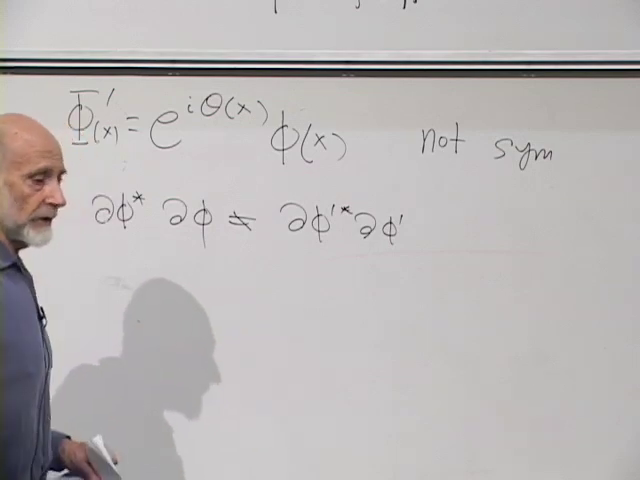
\includegraphics[width=0.78\textwidth]{lecture_08_figure_04.png}\caption{칠판에는 국소 위상 변환과 일반 미분 항이 불변성을 유지하지 못하는 과정이 적혀 있다.}\lectureframe{00:46:49}\label{fig:l08-local-not-symmetry}\end{figure}

벡터 퍼텐셜을 도입하고 하나의 규약을 일관되게 정하자.
\begin{equation}
  D_\mu=\partial_\mu+i g A_\mu,
  \qquad
  A_\mu'=A_\mu-\frac1g\partial_\mu\theta.
  \label{eq:l08-covariant-convention}
\end{equation}
이제
\begin{align}
  D_\mu'\phi'
  &=
  \left(\partial_\mu+i g A_\mu'\right)
  e^{i\theta}\phi
  \notag\\
  &=
  e^{i\theta}
  \left[
    \partial_\mu\phi+i(\partial_\mu\theta)\phi
    +i g A_\mu\phi-i(\partial_\mu\theta)\phi
  \right]
  \notag\\
  &=e^{i\theta}D_\mu\phi.
  \label{eq:l08-covariant-transform}
\end{align}
원치 않는 항들이 상쇄된다. 켤레 미분은
\begin{equation}
  (D_\mu\phi)^*
  =(\partial_\mu-i g A_\mu)\phi^*,
\end{equation}
이며, 그 반대 위상은 곱에서 상쇄된다.
\begin{equation}
  (D_\mu\phi)^*D^\mu\phi.
\end{equation}

\begin{classroomqa}\audiencequestion{지난 강의에서는 게이지장 변환을 반대 부호로 썼나요?\lecturetimestamp{00:48:04}}\lecturerresponse{\(D_\mu\)의 부호와 변환 법칙의 부호를 함께 뒤집는 것은 단지 규약의 차이다. \(D_\mu=\partial_\mu+i gA_\mu\)와 \(\phi'=e^{i\theta}\phi\)를 쓰면 일관성을 위해 \(A_\mu'=A_\mu-g^{-1}\partial_\mu\theta\)이어야 한다. 모든 부호를 함께 바꾸면 다른 규약도 똑같이 잘 작동한다.}\end{classroomqa}

\begin{classroomqa}\audiencequestion{칠판에 \(\phi\)를 대문자 또는 소문자 형태로 쓴 것은 서로 다른 장을 뜻하나요?\lecturetimestamp{00:55:02}}\lecturerresponse{그런 구분은 의도된 것이 아니다. 글자 모양이 바뀐 것은 손글씨 때문이지, 별도의 연산이나 두 번째 스칼라가 있어서가 아니다. 의미 있는 구분은 프라임, 복소켤레 별표, 시공간 지수다.}\end{classroomqa}

\begin{classroomqa}\audiencequestion{운동항에서 복소켤레를 취하는 것은 로런츠 지수를 올리거나 내리는 것과 같은 연산인가요?\lecturetimestamp{00:56:50}}\lecturerresponse{아니다. 별표는 내부 복소장을 켤레화한다. 로런츠 지수는 시공간 계량으로 올린다.
\(D^\mu=g^{\mu\nu}D_\nu\). 로런츠 스칼라를 만들려면 \((D_\mu\phi)^*D^\mu\phi\)와 같이 수축해야 한다. 두 연산은 모두 필요하지만 서로 다른 역할을 한다.}\end{classroomqa}

\subsection{게이지장에는 자체 동역학이 있다}

장세기
\begin{equation}
  F_{\mu\nu}=\partial_\mu A_\nu-\partial_\nu A_\mu
  \label{eq:l08-field-strength}
\end{equation}
는 \(\theta\)의 두 혼합 2계 미분이 서로 상쇄되므로 게이지 불변이다. 시간--공간 성분에는 전기장이, 공간--공간 성분에는 자기장이 들어 있다. 따라서 스칼라 전기역학의 라그랑지언은 다음과 같다.
\begin{equation}
  \mathcal L
  =(D_\mu\phi)^*D^\mu\phi
  -V(\phi^*\phi)
  -\frac14F_{\mu\nu}F^{\mu\nu}.
  \label{eq:l08-abelian-higgs}
\end{equation}
여기서 전하를 띤 장은 보손이다. 페르미온인 전자장은 아니다. 전하를 띤 헬륨 원자핵이나 쿠퍼쌍 응축은 전하를 띤 보손 자유도가 어떻게 생기는지 보여 주는 사례다.

대칭 깨짐 이전에 게이지 항에는 \(A_\mu\)의 미분은 들어 있지만 직접적인 질량 항은 없다. 다음 항을 더하려고 할 수 있다.
\begin{equation}
  \frac12m_A^2A_\mu A^\mu,
\end{equation}
하지만 식~\eqref{eq:l08-covariant-convention} 아래에서
\begin{equation}
  A_\mu A^\mu
  \longmapsto
  \left(A_\mu-\frac1g\partial_\mu\theta\right)
  \left(A^\mu-\frac1g\partial^\mu\theta\right),
  \label{eq:l08-bare-mass-fails}
\end{equation}
가 되어 \(A_\mu A^\mu\)와 같지 않다. 맨 게이지 보손 질량은 국소 대칭에 의해 금지된다.

\begin{figure}[htbp]\centering
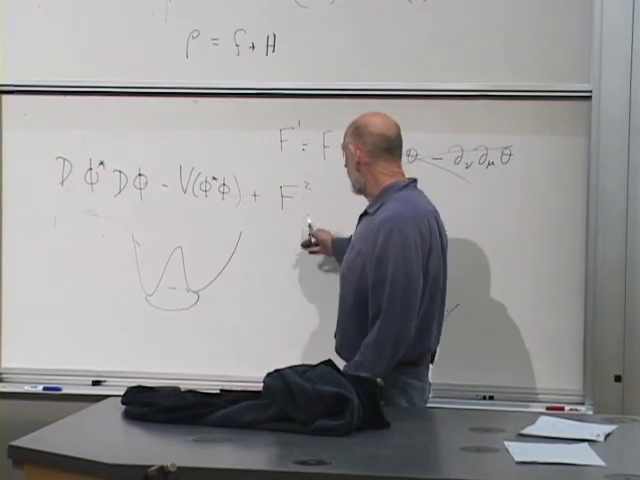
\includegraphics[width=0.76\textwidth]{lecture_08_figure_05.png}\caption{장애를 보여 주는 검증된 칠판 내용: 게이지 변환 아래에서 \(A_\mu A^\mu\)는 \(\partial_\mu\theta\)를 포함하는 제곱식으로 바뀌므로 맨 벡터 질량 항은 불변이 아니다.}\lectureframe{01:07:30}\label{fig:l08-bare-mass-board}\end{figure}

\section{힉스 메커니즘}

\subsection{공변 미분이 질량을 만든다}

깨진 퍼텐셜로 돌아가 정규화가 표준인 매개화를 사용하자.
\begin{equation}
  \phi(x)=\frac{f+h(x)}{\sqrt2}
  e^{i\pi(x)/f}.
\end{equation}
공변 미분은
\begin{equation}
  D_\mu\phi
  =
  \frac{e^{i\pi/f}}{\sqrt2}
  \left[
    \partial_\mu h
    +i(f+h)
      \left(\frac{\partial_\mu\pi}{f}+gA_\mu\right)
  \right].
  \label{eq:l08-covariant-polar}
\end{equation}
이므로
\begin{equation}
\begin{aligned}
  (D_\mu\phi)^*D^\mu\phi
  ={}&
  \frac12(\partial_\mu h)^2
  \\
  &+\frac12(f+h)^2
    \left(\frac{\partial_\mu\pi}{f}+gA_\mu\right)
  \\
  &\hspace{4.2em}\times
    \left(\frac{\partial^\mu\pi}{f}+gA^\mu\right).
\end{aligned}
  \label{eq:l08-higgs-kinetic}
\end{equation}

결정적인 항은 어떤 게이지를 선택하기도 전에 나타난다.
\begin{equation}
  \frac12g^2f^2 A_\mu A^\mu.
  \label{eq:l08-vector-mass-term}
\end{equation}
이를 프로카 형식 \(\frac12m_A^2A_\mu A^\mu\)과 비교하면 다음을 얻는다.
\begin{equation}
  \boxed{m_A=g f}.
  \label{eq:l08-vector-mass}
\end{equation}
같은 전개에서 상호작용 항 \(g^2fh A_\mu A^\mu\)과 \(\frac12g^2h^2A_\mu A^\mu\)도 생긴다. 따라서 벡터 질량은 게이지 대칭성을 임의로 깨뜨려 도입한 것이 아니다. 평형 크기 \(f\)가 영이 아닌 상에서 게이지 불변 스칼라 운동에너지 항을 계산하면 이 질량이 생긴다.

\begin{figure}[htbp]\centering
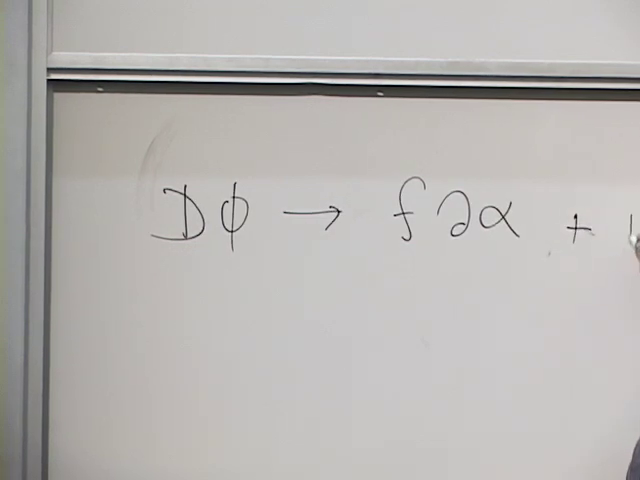
\includegraphics[width=0.78\textwidth]{lecture_08_figure_06.png}\caption{칠판에서 \((D\phi)^*(D\phi)\) 안의 \(f^2A^2\) 기여 항을 따로 뽑아 보인다. 수치 계수는 스칼라장과 게이지 결합을 어떻게 정규화하느냐에 따라 달라진다. 식~\eqref{eq:l08-canonical-polar}와 \eqref{eq:l08-covariant-convention}를 사용하면 결과는 \(m_A=gf\)이다.}\lectureframe{01:10:10}\label{fig:l08-generated-mass-board}\end{figure}

강의에서는 \(g\)와 \(\sqrt2\)의 여러 계수를 칠판 표기 안에 흡수하므로, 질량을 식별하는 대목에서 \(f\), \(2f\), \(\sqrt2f\)를 번갈아 사용한다. 운동항과 퍼텐셜의 정규화를 밝히기 전에는 이 계수들에 불변적인 의미가 없다. 견고한 결과는 \(m_A\propto gf\)이며, 식~\eqref{eq:l08-vector-mass}은 여기서 사용한 규약에 따른 계수를 준다.

\subsection{위상을 흡수하기}

게이지 변환 아래에서 위상 변수는 다음과 같이 변한다.
\begin{equation}
  \pi'(x)=\pi(x)+f\,\theta(x).
\end{equation}
다음과 같이 택하자.
\begin{equation}
  \theta(x)=-\frac{\pi(x)}{f}.
  \label{eq:l08-unitary-gauge-choice}
\end{equation}
그러면 \(\pi'=0\)이다. 이것이 유니터리 게이지이며, 이 게이지에서는 \begin{equation}
  \phi'(x)=\frac{f+h(x)}{\sqrt2}
\end{equation}가 실수다. 식~\eqref{eq:l08-higgs-kinetic}은 다음과 같이 단순해진다.
\begin{equation}
  (D_\mu\phi')^*D^\mu\phi'
  =
  \frac12(\partial_\mu h)^2
  +\frac12g^2(f+h)^2A_\mu'A^{\prime\mu}.
  \label{eq:l08-unitary-gauge-lagrangian}
\end{equation}
각방향 골드스톤 장은 독립 변수 목록에서 사라지지만, 벡터 질량은 남는다.

강의에서는 먼저 저에너지 극한 \(\rho=f\)에서 이를 보인다. 이때
\begin{align}
  \phi&=f e^{i\alpha},
  \notag\\
  D_\mu\phi
  &=if e^{i\alpha}
    \left(\partial_\mu\alpha+gA_\mu\right),
  \notag\\
  (D_\mu\phi)^*
  &=-if e^{-i\alpha}
    \left(\partial_\mu\alpha+gA_\mu\right).
  \label{eq:l08-frozen-radius}
\end{align}
두 식의 곱은
\begin{equation}
  f^2
  \left(\partial_\mu\alpha+gA_\mu\right)
  \left(\partial^\mu\alpha+gA^\mu\right).
\end{equation}
이다. \(\theta=-\alpha\)를 택하면 \(g^2f^2A_\mu'A^{\prime\mu}\)가 남는다.

\begin{figure}[htbp]\centering
\includegraphics[width=0.82\textwidth]{lecture_08_figure_07.png}\caption{반지름을 고정한 완전한 칠판 전개: 공변 미분에는 위상 미분과 벡터 퍼텐셜이 함께 들어 있다. 이어서 강의에서는 \(\theta=-\alpha\)를 택해 위상을 없애고 벡터 질량 항을 남긴다.}\lectureframe{01:16:20}\label{fig:l08-frozen-radius-board}\end{figure}

\begin{classroomqa}\audiencequestion{각방향 모드가 사라지는 것을 명시적으로 보여 주는 변수로 라그랑지언 전체를 다시 쓸 수 있나요?\lecturetimestamp{01:13:49}}\lecturerresponse{그렇다. 극좌표 변수에서는 위상이 게이지 불변 조합 \(\partial_\mu\alpha+gA_\mu\)에만 나타난다. 이 게이지가 잘 정의되는 모든 곳에서 \(\theta=-\alpha\)인 게이지 변환을 택하면 위상을 0으로 만들 수 있다. 그러면 스칼라 운동항은 벡터 질량 항이 되고, 게이지 불변 장세기 항은 변하지 않는다.}\end{classroomqa}

\begin{classroomqa}\audiencequestion{\(\alpha\)의 진동은 게이지장의 진동과 구별할 수 없나요?\lecturetimestamp{01:18:02}}\lecturerresponse{게이지 이론에서 이에 대응하는 \(A_\mu\)의 변화로 상쇄되는 \(\alpha\)의 순수한 변화는 서로 다른 물리적 파동이 아니라 게이지에 따른 재기술이다. 불변량은 \(\partial_\mu\alpha+gA_\mu\)다. 전역 골드스톤 장으로 표현되던 물리적 모드는 질량 있는 벡터의 종방향 편광으로 다시 나타난다.}\end{classroomqa}

국소 게이지 대칭성이 자발적으로 깨진다고 흔히 말한다. 게이지를 선택한 뒤 스칼라장이 영이 아닌 진공값을 갖고 스펙트럼에 질량이 있는 벡터가 포함된다는 점에서 이 표현은 실용적으로 유용하다. 그러나 엄밀히 말해 게이지 변환은 서로 다른 물리적 상태가 아니라 중복된 기술들을 서로 대응시킨다.
\editorialnote{국소 게이지 중복성은 전역 대칭성과 같은 게이지 불변적 의미에서 깨지는 것이 아니다. 정확히 말하면 이론은 힉스 상에 있다. 게이지 고정 섭동 이론에서는 이 상을 영이 아닌 스칼라 기댓값과 그에 따른 질량 있는 벡터 스펙트럼으로 기술한다.}

\section{골드스톤 자유도는 어디로 갔는가}

변수를 바꾸었다고 해서 물리적인 것이 사라질 수는 없다. 힉스 상에 들어가기 전후의 자유도를 세어 보자.

그 전에는
\begin{equation}
  \underbrace{2}_{\text{massless vector}}
  +
  \underbrace{2}_{\text{complex scalar}}
  =4.
\end{equation}
질량 없는 벡터에는 횡편광이 두 개 있다. 복소 스칼라에는 방사 방향과 각방향의 두 실수 성분이 있다.

그 뒤에는
\begin{equation}
  \underbrace{3}_{\text{massive vector}}
  +
  \underbrace{1}_{\text{radial Higgs}}
  =4.
  \label{eq:l08-degree-count}
\end{equation}
질량 있는 벡터는 정지 상태로 만들 수 있다. 정지계에서는 특별히 선택되는 공간 방향이 없으므로 편광 상태가 세 개여야 한다. 벡터가 움직일 때 그중 둘은 횡방향이고 하나는 종방향이다. 골드스톤 모드는 이 종방향 편광이 되었다.

\begin{figure}[htbp]\centering
\begin{adjustbox}{max width=\linewidth}\begin{tikzpicture}[x=1cm,y=1cm]
  \node[draw,rounded corners,fill=blue!7,minimum width=4.3cm,
        minimum height=2.1cm,align=center] (before) at (0,0)
    {massless \(A_\mu\): \(2\) transverse\\
     \(+\)\\
     complex \(\phi\): \(h+\pi\)};
  \node[draw,rounded corners,fill=orange!10,minimum width=4.3cm,
        minimum height=2.1cm,align=center] (after) at (7,0)
    {massive \(A_\mu\): \(2\) transverse\\
     \(+\;1\) longitudinal\\
     \(+\) radial \(h\)};
  \draw[->,very thick] (before) -- node[above]{Higgs phase} (after);
  \draw[->,teal!70!black,thick]
    (-0.15,-0.65) to[bend right=28]
    node[below,align=center]{Goldstone \(\pi\) supplies\\longitudinal mode}
    (6.8,-0.65);
\end{tikzpicture}\end{adjustbox}\caption{힉스 메커니즘은 물리적 자유도를 없애는 것이 아니라 재배열한다.}\label{fig:l08-degree-rearrangement}\end{figure}

\begin{classroomqa}\audiencequestion{자유도 수를 어기지 않으면서 각방향 자유도가 어떻게 사라질 수 있나요?\lecturetimestamp{01:19:13}}\lecturerresponse{물리적으로 사라지는 것은 아니다. 질량 없는 벡터는 정지 상태로 만들 수 없기 때문에 헬리시티가 두 개다. 질량 있는 벡터에는 종방향을 포함해 편광 상태가 세 개 있다. 골드스톤 모드가 세 번째 편광이 되므로 전체 자유도 수는 그대로다.}\end{classroomqa}

강의에서는 유용한 운동학적 검증 방법을 제시한다. 질량이 있는 벡터 입자를 생각해 정지 상태까지 감속한 다음 새로운 방향으로 가속한다고 하자. 원래 운동 방향에 대해 횡방향이던 편광이 새로운 운동 방향에 대해서는 종방향이 될 수 있다. 마찬가지로 원편광된 질량 있는 입자를 정지 상태로 옮겼다가 반대 방향으로 보내면 헬리시티 표지가 뒤집힌다. 엄밀히 질량이 없는 입자는 어떤 관성계에서도 정지 상태가 될 수 없으므로 이 실험을 거칠 수 없다. 따라서 그 두 헬리시티는 일관된 물리적 스펙트럼을 이룬다.

\section{초전도체와의 유사성}

일반적인 초전도체에서는 전자들이 쿠퍼 쌍을 이룬다. 쿠퍼 쌍은 전하 \(2e\)를 띤 보손이며, 응축체는 전하를 띤 복소 질서 매개변수로 기술된다. 그 크기가 영이 아니면 질서 매개변수의 위상과 전자기 벡터 퍼텐셜의 결합으로 앤더슨--힉스 메커니즘이 나타난다. 정적 자기장은 런던 침투 깊이를 따라 감쇠하므로 초전도체 내부로 자유롭게 뻗어 나가지 않는다. 이처럼 특정 매질에 한정된 정확한 의미에서 광자는 질량을 얻은 것처럼 거동한다.

이 사례는 처음에 제시한 구분도 명확히 해 준다. 전자기장이 영구적으로 다른 기본 입자로 바뀌는 것은 아니다. 질량 있는 전파 법칙은 물질 내부의 집단 상태에 해당하며, 바깥의 진공 광자는 여전히 질량이 없다.

\section{확립된 결과}

논리를 유지하면서 이제 논증을 간결하게 정리할 수 있다.
\begin{enumerate}
  \item 깨진 전역 연속 대칭성에는 평평한 각방향이 있으므로 질량이 없는 골드스톤 모드가 존재한다.
  \item 국소 위상 불변성은 게이지 퍼텐셜을 요구하며 \(\partial_\mu\)를 \(D_\mu\)로 대체한다.
  \item 맨 \(A_\mu A^\mu\) 질량은 국소 변환 법칙을 위반한다.
  \item 전하를 띤 스칼라의 평형 크기 \(f\)가 영이 아니면 게이지 불변 항 \(|D_\mu\phi|^2\)에 \(\frac12g^2f^2A_\mu A^\mu\)가 포함된다.
  \item 게이지를 선택하면 위상을 제거할 수 있으며, 그 물리적 자유도는 질량이 있는 벡터의 종방향 편극이 된다.
  \item 방사 방향 힉스 여기자의 질량은 스칼라 퍼텐셜의 곡률로 정해진다.
\end{enumerate}

다음 과제는 페르미온에 질량을 부여하는 것이다. 전자와 쿼크에는 벡터 메커니즘을 직접 적용할 수 없다. 이들의 힉스 결합은 유카와 상호작용이다. 스칼라장이 \(f\)에 자리 잡으면 이 상호작용은 페르미온 질량 항이 된다.

전약 대칭성 깨짐이 없으면 익숙한 입자들이 질량이 없었을 것이라는 폭넓은 진술에는 마지막으로 단서를 붙여야 한다. 기본 입자인 쿼크와 하전 렙톤의 질량, 그리고 \(W\) 및 \(Z\)의 질량은 힉스 기댓값이 영이 되면 사라진다. 그러나 양성자와 중성자 질량의 대부분은 쿼크의 힉스 질량이 아니라 QCD 가둠과 강한 장의 에너지에서 동역학적으로 비롯된다. 이 구분은 여기서 유도한 힉스 메커니즘을 바꾸지 않으며, 그 적용 범위를 정확히 한정해 준다.

\chapter{페르미온 질량: 카이랄성, 유카와 결합, 마요라나 중성미자}

\lectureoverview{먼저 장난감 \(U(1)\) 이론에서 게이지 보손의 힉스 메커니즘을 다시 살펴본 뒤, 페르미온에 대해서도 이에 대응하는 질문을 던진다. 디랙 질량은 왼쪽 카이랄 장과 오른쪽 카이랄 장을 섞지만, 약한 상호작용은 이들에 서로 다른 전하를 부여하므로 맨 질량항을 허용하지 않는다. 힉스 장과의 유카와 결합은 대칭성을 보존한다. 힉스 장이 진공 기댓값을 얻으면 같은 상호작용이 페르미온 질량이 되고, 측정 가능한 힉스--페르미온 결합으로 나타난다. 마지막 부분에서는 이 논리를 따라 중성미자 질량, 보호받지 못하는 무거운 입자의 가능성, 우주선의 운동학, 상대론적 관성, 중력을 살펴본다.}

도입부의 복습은 앞선 강의를 그저 되풀이하기 위한 것이 아니다. 그 내용에서 페르미온에도 적용할 수 있는 개념 하나를 가져와야 한다. 질량은 운동량이 영인 들뜸에 대응하는 영이 아닌 에너지다. 장에서 운동량이 영이라는 것은 파장이 무한대이거나 변위가 모든 곳에서 같다는 뜻이다. 미분항만 있는 이론은 균일한 변위를 감지할 수 없다. 미분항이 없는 항은 감지할 수 있다.

\section{한 번에 살펴보는 게이지 보손 이야기}

\subsection{미분 에너지와 질량 없는 벡터장}

모형 게이지 장은 \(A_\mu\)이고, 장세기는 다음과 같다.
\begin{equation}
  F_{\mu\nu}
  =\partial_\mu A_\nu-\partial_\nu A_\mu .
  \label{eq:l09-field-strength}
\end{equation}
판서에서는 게이지 운동항을 개략적으로 \(F^2\)라고 쓴다. 표준적인 정규화를 적용하면 다음과 같다.
\begin{equation}
  \mathcal L_{\mathrm{gauge}}
  =-\frac14 F_{\mu\nu}F^{\mu\nu}.
  \label{eq:l09-gauge-kinetic}
\end{equation}

\begin{figure}[htbp]
\centering
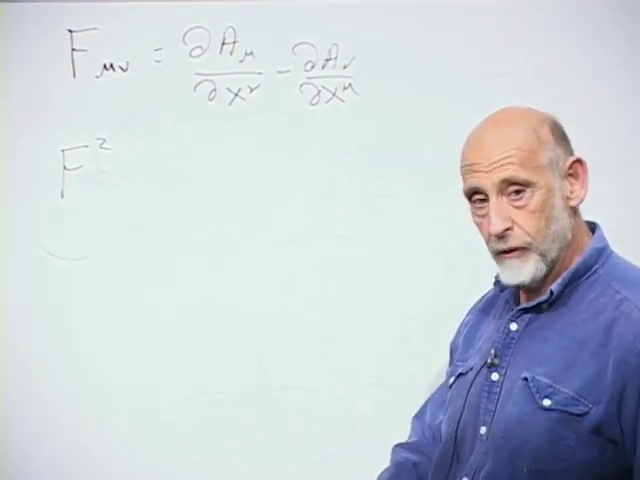
\includegraphics[width=0.72\textwidth]{lecture_09_figure_02.png}
\caption{게이지 장의 장세기 정의와 게이지 장의 미분 에너지를 나타내는 판서의 \(F^2\) 약식 표기.}
\lectureframe{00:02:39}
\label{fig:l09-field-strength-board}
\end{figure}

\(A_\mu\)는 \eqref{eq:l09-gauge-kinetic}에서 나타날 때마다 미분된다. 따라서
\begin{equation}
  A_\mu(x)\longmapsto A_\mu(x)+c_\mu,
  \qquad \partial_\nu c_\mu=0,
\end{equation}
는 \(F_{\mu\nu}\)를 바꾸지 않는다. 그러므로 균일한 벡터 퍼텐셜에는 장세기 에너지가 들지 않는다. 강의의 표현을 빌리면, 운동량이 0인 모드에는 갭이 없고 게이지 보손은 질량이 없다.

이 \(U(1)\) 장은 의도적으로 단순화한 대용물이다. 실제 대상은 전자기 광자가 아니라 \(W^\pm\)와 \(Z\)이다. 깨지지 않은 전자기 대칭성은 광자를 질량 없는 상태로 두지만, 깨진 전약 대칭성은 약한 게이지 보손에 질량을 부여한다.

\subsection{힉스장의 반지름을 고정하기}

전하를 띤 복소 스칼라장을 도입하고 극형식으로 쓰면,
\begin{equation}
  \phi(x)=\rho(x)e^{i\alpha(x)}.
\end{equation}
멕시코 모자형 퍼텐셜은 반지름이 영이 아닌 원 위에서 최소가 된다. 그 반지름을 \(f\)라 하자. 반지름 방향은 비교적 강직하다. 우선 반지름은 고정하고 위상만 남겨 두자.
\begin{equation}
  \phi(x)\simeq f e^{i\alpha(x)}.
  \label{eq:l09-frozen-higgs}
\end{equation}

\begin{figure}[htbp]
\centering
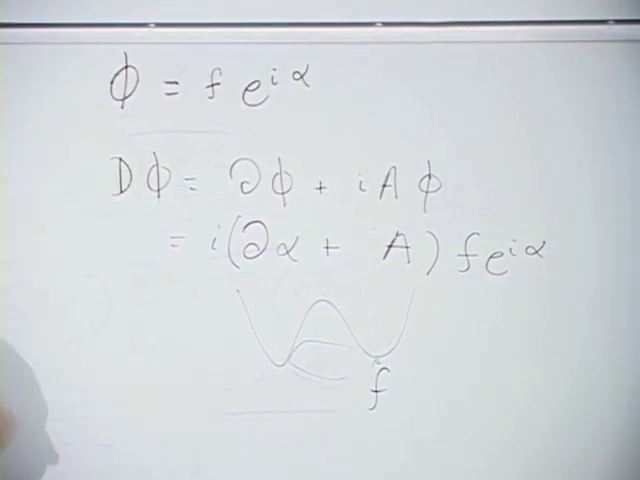
\includegraphics[width=0.72\textwidth]{lecture_09_figure_03.png}
\caption{고정된 힉스 반지름과 그 공변미분, 그리고 복습에서 사용한 깨진 퍼텐셜의 간략한 그림.}
\lectureframe{00:06:42}
\label{fig:l09-frozen-board}
\end{figure}

다음 규약을 택하자.
\begin{equation}
\begin{aligned}
  D_\mu&=\partial_\mu+igA_\mu,
  \\
  \phi&\longmapsto e^{i\theta}\phi,
  \\
  A_\mu&\longmapsto A_\mu-\frac1g\partial_\mu\theta .
\end{aligned}
  \label{eq:l09-gauge-convention}
\end{equation}
강의에서는 \(g\)를 생략하지만, 이를 드러내 두면 차원과 최종 질량을 분명히 알 수 있다. 고정된 장에 작용시키면
\begin{align}
  D_\mu\phi
  &=(\partial_\mu+igA_\mu)f e^{i\alpha}
  \notag\\
  &=i\bigl(\partial_\mu\alpha+gA_\mu\bigr)
    f e^{i\alpha}.
  \label{eq:l09-covariant-frozen}
\end{align}
복소켤레를 곱하면 위상이 사라지고, \(i\)와 \(-i\)의 곱도 \(+1\)이 된다.
\begin{equation}
  |D_\mu\phi|^2
  =f^2
   \bigl(\partial_\mu\alpha+gA_\mu\bigr)
   \bigl(\partial^\mu\alpha+gA^\mu\bigr).
  \label{eq:l09-frozen-square}
\end{equation}

\begin{classroomqa}\audiencequestion{미분에서 \(i\)가 나오므로 공변미분의 제곱에는 음의 부호가 붙어야 하나요?
\lecturetimestamp{00:07:39}}\lecturerresponse{아니다. 운동항은 복소켤레와 곱한 것이다. 한 인자에서는 \(i\)가, 다른 인자에서는 \(-i\)가 나오므로 \(i(-i)=1\)이다. \(D_\mu\)의 부호 규약은 일관되게 뒤집을 수 있지만, 이에 대응하는 에너지 식에서 절댓값의 제곱은 양수다.}\end{classroomqa}

\eqref{eq:l09-frozen-square}의 조합 자체가 이동된 게이지 장이다. \(\theta=-\alpha\)를 택해 스칼라 위상을 없애고, 다음과 같이 정의하자.
\begin{equation}
  A'_\mu=A_\mu+\frac1g\partial_\mu\alpha .
  \label{eq:l09-unitary-gauge-field}
\end{equation}
그러면
\begin{equation}
  |D_\mu\phi|^2=g^2f^2 A'_\mu A'^\mu .
  \label{eq:l09-vector-mass-term}
\end{equation}
새 항에는 \(A'_\mu\)의 미분이 없다. 이제 균일한 장에도 에너지가 저장되므로, 운동량이 0인 벡터 모드에는 갭이 생긴다.

\begin{figure}[htbp]
\centering
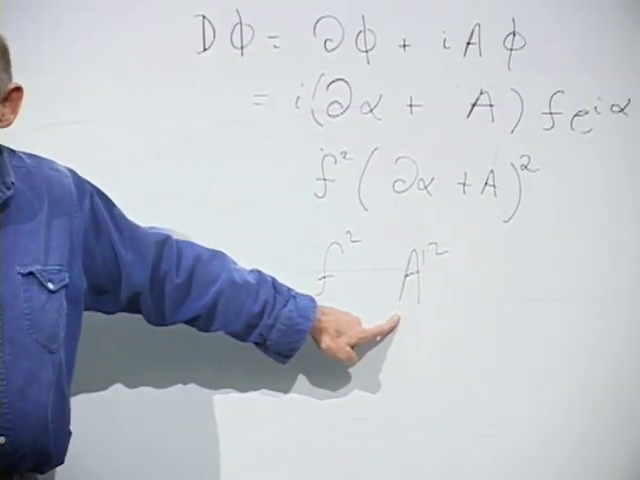
\includegraphics[width=0.72\textwidth]{lecture_09_figure_04.png}
\caption{위상을 흡수한 뒤 게이지 보손 질량이 생겼음을 나타내는 \(f^2A^2\) 항을 판서에서 따로 보여준다.}
\lectureframe{00:10:31}
\label{fig:l09-vector-mass-board}
\end{figure}

스칼라장을 표준적으로 정규화하면
\(\phi=(f+h)e^{i\pi/f}/\sqrt2\)로 쓴다. 이를 벡터 항 \(\tfrac12m_A^2A_\mu A^\mu\)와 비교하면 이 아벨 모형에서
\begin{equation}
  m_A=gf
  \label{eq:l09-abelian-vector-mass}
\end{equation}
을 얻는다. 강의에서는 정규화 인자를 생략하고 벡터 질량이 \(f\)로 정해진다고 요약한다.

위상 모드가 아무런 설명 없이 사라진 것은 아니다. 게이지화하기 전에는 질량 없는 골드스톤 보손이었다. 게이지화한 뒤에는 질량 있는 벡터 입자에 필요한 종방향 편광을 제공한다. 잠시 고정해 두었던 반지름 방향 요동은 물리적인 힉스 들뜸으로 남는다.

\subsection{미분이 없는 항은 왜 질량을 뜻하는가}

\begin{classroomqa}\audiencequestion{\(A'^2\) 항은 왜 단순히 또 다른 상호작용이 아니라 질량으로 간주되나요?
\lecturetimestamp{00:13:10}}\lecturerresponse{질량은 정지 상태의 에너지다. 장에서 정지한 입자는 운동량이 0이고 파장이 무한대인 모드의 양자다. 미분항은 정적으로 균일한 변위에 에너지를 주지 않지만, \(m_A^2A'^2\)는 에너지를 준다. 운동량이 0일 때 생기는 이 비영 에너지가 정지 에너지 갭이다.}\end{classroomqa}

강의에서는 이 내용을 세 가지 역학적 비유로 설명한다.

\begin{itemize}
  \item 결정에서는 이웃한 원자들이 서로 다르게 이동하므로, 변위가 위치에 따라 천천히 변해도 탄성 에너지가 든다. 모든 원자를 함께 옮기는 강체 병진에는 내부 에너지가 들지 않는다. 따라서 음향 포논은 갭이 없다.
  \item 이상적으로 회전 대칭인 자석에서는 스핀 방향이 공간에 따라 변하면 교환 에너지가 들지만, 모든 스핀을 함께 회전시키는 데는 에너지가 들지 않는다. 이에 대응하는 장파장 스핀파는 갭이 없다.
  \item 플라스마에서 전자 유체를 양전하 배경에 대해 이동시키면, 상대 변위가 균일하더라도 전하 분리가 생기고 복원 전기장이 형성된다. 그 결과 플라스몬은 파수가 영일 때도 영이 아닌 진동수를 갖는다.
\end{itemize}

힉스 메커니즘으로 질량을 얻은 게이지 장은 세 번째 사례와 같이 거동한다. 깨진 매질은 그렇지 않았다면 에너지가 들지 않았을 균일한 변위에 저항한다.

\begin{classroomqa}\audiencequestion{게이지 장을 도입하기 전에도 위상 \(\alpha\)는 이미 진동하지 않았나요?
\lecturetimestamp{00:18:24}}\lecturerresponse{진동했다. 그 에너지는 \(f^2(\partial_\mu\alpha)^2\)에 비례했다. 위치마다 달라지는 위상에는 기울기 에너지가 있어 전파될 수 있지만, 균일한 위상 변화에는 에너지가 들지 않는다. 이것이 바로 질량 없는 골드스톤 모드다.}\end{classroomqa}

\begin{classroomqa}
\audiencequestion{미분에는 시간 미분도 포함됩니다. 격자 전체를 실제로 움직이거나 장 전체를 변화시키면 운동 에너지가 생기지 않나요?\lecturetimestamp{00:22:18}}
\lecturerresponse{그렇습니다. 여기서 비교하는 것은 정적인 배치들이거나 원하는 만큼 천천히 준비한 배치들입니다. 격자가 영이 아닌 속도로 병진하면 운동 에너지가 있습니다. 질량을 판별할 때 묻는 것은 배치가 정지해 있고 공간적으로 균일해도 에너지가 남는가 하는 점입니다.}
\end{classroomqa}

\section{실험적 단서: 약한 상호작용은 왼쪽과 오른쪽을 구별한다}

이제 강의는 전자, 뮤온, 쿼크를 살펴본다. 이들의 질량도 힉스 장에서 비롯되지만, 페르미온 질량은 이차 벡터 항이 아니므로 메커니즘의 형태가 다르다. 페르미온 질량은 두 카이랄 장 사이의 결합이다.

\subsection{베타 붕괴에서의 패리티 위반}

먼저 약한 상호작용이 패리티를 위반한다는 실험적 사실에서 출발하자. 양자전기역학과 양자색역학에서는 어떤 과정과 그 거울상이 똑같이 다뤄진다. 약한 상호작용은 그렇지 않다. 중성자 베타 붕괴에서는
\begin{equation}
  n\longrightarrow p+e^-+\bar\nu_e,
  \label{eq:l09-beta-decay}
\end{equation}
전하 전류 상호작용이 선택하는 고에너지 전자의 헬리시티가 왼손잡이다. 즉 스핀은 운동량과 반대 방향을 향한다. 이에 대응하는 반중성미자의 헬리시티는 반대다.

초상대론적 입자의 헬리시티를 다음과 같이 정의하자.
\begin{equation}
  h=\frac{\bm S\cdot\bm p}{|\bm S|\,|\bm p|}.
\end{equation}
스핀과 운동량이 나란하면 \(h=+1\)이고, 서로 반대 방향이면 \(h=-1\)이다. 약한 상호작용은 왼쪽 카이랄 전자 장과 왼쪽 카이랄 중성미자 장에 결합하며, 오른쪽 카이랄 전자 장에는 같은 방식으로 결합하지 않는다.\editorialnote{강의에서는 고에너지에서 시각적으로 직관적이라는 이유로 처음에 헬리시티의 의미로 손잡이성을 사용한다. 그러나 게이지 전하는 카이랄성, 즉 \(P_L=(1-\gamma^5)/2\)와 \(P_R=(1+\gamma^5)/2\)가 선택하는 로런츠 표현의 표지에 작용한다. 질량 없는 입자에서는 입자의 카이랄성과 헬리시티가 일치하지만, 질량 있는 입자에서는 그렇지 않다.}

전체 \(SU(2)_L\times U(1)_Y\) 장부를 다루지 않고도 장애물을 드러내기 위해, 관련 전하를 \(\psi_L\)만 갖는 가상의 \(U(1)\) 세계를 생각해 보자.
\begin{equation}
  \psi_L\longmapsto e^{i\theta}\psi_L,
  \qquad
  \psi_R\longmapsto\psi_R .
  \label{eq:l09-chiral-toy-charge}
\end{equation}
이는 전자기 이론이 아니다. 실제로 왼쪽과 오른쪽 카이랄 전자는 같은 전기 전하를 갖는다. 이는 두 카이랄성이 서로 다른 전약 표현에 속하는 약한 상호작용을 단순화해 그린 것이다.

\begin{classroomqa}\audiencequestion{쿼크에도 같은 왼쪽--오른쪽 비대칭이 적용되나요?
\lecturetimestamp{00:31:50}}\lecturerresponse{그렇다. 단, 알맞은 약한 다중항과 초전하를 고려해야 한다. 왼쪽 카이랄 업형 및 다운형 쿼크는 약한 이중항을 이루지만, 오른쪽 카이랄 장은 약한 단일항이다. 따라서 쿼크의 힉스 결합에도 전자의 경우와 같은 구조적 문제가 생긴다.}\end{classroomqa}

\section{디랙 질량은 왼쪽--오른쪽 혼합이다}

\subsection{4성분 방정식에서 두 바일 방정식으로}

디랙 파동함수는 네 성분을 갖는다. 대략 말해 두 성분은 스핀을 나타내고, 나머지 두 성분은 양에너지 해와 음에너지 해를 구별하며, 음에너지 해는 반입자 자유도로 다시 해석된다. 해밀토니안 형식으로 쓰면
\begin{equation}
  i\frac{\partial\Psi}{\partial t}
  =\left(-i\bm\alpha\cdot\bm\nabla+m\beta\right)\Psi .
  \label{eq:l09-dirac-hamiltonian}
\end{equation}
행렬 \(\alpha_i\)와 \(\beta\)는 에너지, 운동량, 질량 사이의 상대론적 관계를 나타낸다.

\begin{figure}[htbp]
\centering
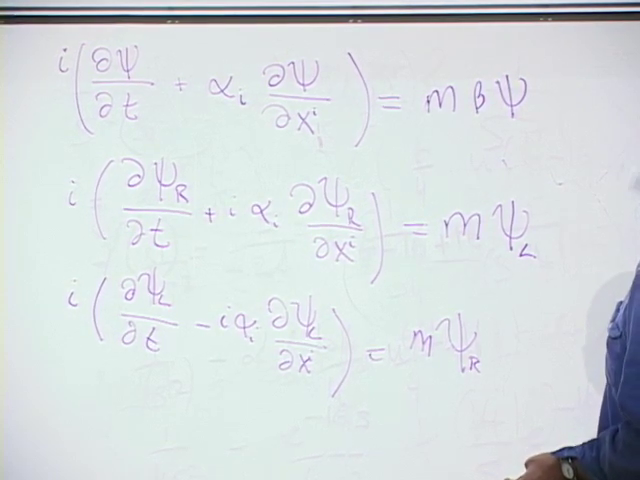
\includegraphics[width=0.74\textwidth]{lecture_09_figure_05.png}
\caption{판서에서는 먼저 디랙 방정식을 쓴 다음, 이를 결합된 왼쪽 및 오른쪽 손잡이 방정식으로 나눈다.}
\lectureframe{00:40:30}
\label{fig:l09-dirac-board}
\end{figure}

카이랄 기저를 쓰면 \(m\)의 역할이 명확해진다. \(\sigma^\mu=(1,\bm\sigma)\)와 \(\bar\sigma^\mu=(1,-\bm\sigma)\)를 두면
\begin{align}
  i\bar\sigma^\mu\partial_\mu\psi_L&=m\psi_R,
  \label{eq:l09-weyl-left}\\
  i\sigma^\mu\partial_\mu\psi_R&=m\psi_L.
  \label{eq:l09-weyl-right}
\end{align}
\(m=0\)일 때 두 방정식은 서로 독립이다. 왼쪽 카이랄 장과 오른쪽 카이랄 장은 서로 영향을 주지 않고 전파될 수 있다. \(m\neq0\)일 때는 각 장이 다른 장의 원천으로 나타난다. 이것이 디랙 질량이 왼쪽과 오른쪽을 섞는다는 말의 정확한 의미다.

Susskind는 이를 페르미온이 왼쪽과 오른쪽 사이에서 진동한다고 설명한다. 이 표현은 결합을 잘 나타내지만, 점입자가 고전적으로 앞뒤로 뒤집힌다는 뜻으로 받아들여서는 안 된다. 정확한 진술은 결합된 장 방정식 \eqref{eq:l09-weyl-left}--\eqref{eq:l09-weyl-right}이다.

\begin{classroomqa}\audiencequestion{판서에 나온 두 방정식의 \(i\) 인자와 부호는 서로 일관되나요?
\lecturetimestamp{00:41:10}}\lecturerresponse{판서의 줄마다 일관되지는 않는다. 빠르게 유도하는 과정에서 \(i\) 하나를 일관성 없이 바깥으로 뺐다. 신뢰할 수 있는 내용은 결합 구조다. 방정식 \eqref{eq:l09-weyl-left}과 \eqref{eq:l09-weyl-right}은 표준적인 일관된 규약 하나를 제시한다.}\end{classroomqa}

\subsection{약한 대칭성은 왜 맨 질량항을 금지하는가}

이에 대응하는 디랙 질량항은 라그랑지안에서
\begin{equation}
  \mathcal L_m
  =-m\bar\psi\psi
  =-m\left(\bar\psi_L\psi_R+\bar\psi_R\psi_L\right).
  \label{eq:l09-bare-dirac-mass}
\end{equation}
이다. 장난감 변환 \eqref{eq:l09-chiral-toy-charge} 아래에서
\begin{equation}
  \bar\psi_L\psi_R\longmapsto
  e^{-i\theta}\bar\psi_L\psi_R,
  \qquad
  \bar\psi_R\psi_L\longmapsto
  e^{i\theta}\bar\psi_R\psi_L.
\end{equation}
두 항 중 어느 것도 불변이 아니다. 따라서 대칭성이 깨지기 전에는 직접적인 왼쪽--오른쪽 혼합 계수 \(m\)가 금지된다.

전자기 상호작용만으로는 이 문제가 생기지 않는다. \(\psi_L\)와 \(\psi_R\)의 전기 전하가 같기 때문이다. 장애물은 이들의 약한 양자수가 서로 다르다는 데서 생긴다.

\subsection{카이랄성의 미묘함을 드러내는 헬리시티 질문}

이제 수업에서는 직관적인 손잡이성 그림을 여러 각도에서 살펴본다. 이 질문들은 부수적인 문제가 아니다. 헬리시티가 유용한 경우와 카이랄성으로 대신해야 하는 경우를 정확히 드러낸다.

\begin{classroomqa}\audiencequestion{약한 상호작용이 두 헬리시티의 전자를 똑같은 비율로 방출한다면 세계는 어떻게 달라질까요?
\lecturetimestamp{00:42:12}}\lecturerresponse{그 과정에서 나타나는 직접적인 패리티 비대칭은 사라질 것이다. 그러나 실제 전약 이론은 카이랄 이론이다. 전하 약한 상호작용을 하는 것은 왼쪽 카이랄 이중항뿐이다. 자연이 왜 이런 구조를 택했는지에 대한 더 자세한 설명은 강의 후반으로 미룬다.}\end{classroomqa}

\begin{classroomqa}\audiencequestion{전자의 스핀을 수직 방향으로 준비한 뒤 전자를 수평 방향으로 가속한다고 합시다. 이 전자는 왼손잡이인가요, 오른손잡이인가요?
\lecturetimestamp{00:42:44}}\lecturerresponse{운동량에 수직인 스핀 상태는 두 헬리시티 상태의 중첩이다. 스핀이 운동량과 나란하거나 반대 방향일 때에만 헬리시티가 정해진다. 그럼에도 카이랄 투영자는 장에 대해 잘 정의되어 있다.}\end{classroomqa}

질량 있는 입자는 정지 상태까지 감속한 뒤, 스핀은 뒤집지 않고 반대 방향으로 가속할 수 있다. 그러면 헬리시티의 부호가 바뀐다. 질량 없는 입자는 로런츠 부스트로 앞질러지거나 정지 상태가 될 수 없으므로, 적절한 부스트 아래에서 헬리시티가 불변이다. 이 점에서 강의는 물리적인 헬리시티가 하나뿐인 종은 질량이 없어야 한다고 말한다. 장 이론의 더 정확한 진술은 로런츠 불변 디랙 질량에 두 카이랄성이 모두 필요하다는 것이다.

\begin{classroomqa}\audiencequestion{원편광된 광자가 거울에 반사되어 방향을 바꾸고도 정지하지 않을 수 있습니다. 이것은 헬리시티 논리와 모순되지 않나요?
\lecturetimestamp{00:45:28}}\lecturerresponse{아니다. 거울은 각운동량을 주고받으며 진행 방향을 바꿀 수 있는 외부 계다. 반사 과정은 광자를 앞지르는 로런츠 부스트가 아니다. 반사 채널의 존재 여부는 허용되는 편광 상태와 물질의 경계 조건에도 달려 있다.}\end{classroomqa}

\begin{classroomqa}\audiencequestion{일반적인 전자 빔에는 한 가지 손잡이성만 있나요, 둘 다 있나요?
\lecturetimestamp{00:46:10}}\lecturerresponse{대체로 둘 다 있다. 질량 있는 전자 상태에는 두 카이랄 성분이 모두 들어 있으며, 비편극 빔에는 두 헬리시티가 모두 포함된다. 특수한 선원으로 헬리시티 비대칭이 큰 편극 빔을 만들 수도 있다.}\end{classroomqa}

\begin{classroomqa}\audiencequestion{스핀과 관계없이 빔의 초점을 맞출 수 있나요, 아니면 자기장이 두 편광을 분리하나요?
\lecturetimestamp{00:46:29}}\lecturerresponse{일반적인 위치 초점 조절은 스핀에 거의 무관할 수 있지만, 자기 모멘트는 자기장 기울기와 결합한다. 따라서 스핀 선택 선원, 슈테른--게를라흐형 기울기, 가속기에서의 스핀 동역학을 이용해 편광을 준비하거나 분리할 수 있다.}\end{classroomqa}

\begin{classroomqa}\audiencequestion{왼쪽과 오른쪽에 대한 약한 상호작용의 차이는 그저 우연인가요?
\lecturetimestamp{00:48:13}}\lecturerresponse{이 강의의 범위에서는 표준모형에 포함된 실험적 사실이다. 아무렇게나 생긴 우연이라고 보기에는 너무 체계적이지만, 표준모형 자체는 카이랄 전하의 전체 패턴을 더 깊은 원리에서 유도하지 않는다.}\end{classroomqa}

\section{유카와 메커니즘}

\subsection{빠진 전하를 힉스가 맡게 하기}

대칭성은 수로 주어지는 질량을 금지하지만, 빠진 변환 위상을 제공하는 장과의 상호작용은 허용한다. 다음 변환을 하는 복소 스칼라를 도입하자.
\begin{equation}
  \phi\longmapsto e^{i\theta}\phi,
  \qquad
  \phi^\dagger\longmapsto e^{-i\theta}\phi^\dagger.
  \label{eq:l09-scalar-charge}
\end{equation}
그러면
\begin{equation}
  \mathcal L_Y
  =-y\,\bar\psi_L\phi\psi_R
   -y^*\,\bar\psi_R\phi^\dagger\psi_L
  \label{eq:l09-yukawa-lagrangian}
\end{equation}
은 게이지 불변이다. 첫 번째 항에서 \(\bar\psi_L\)는 \(e^{-i\theta}\)를, \(\phi\)은 \(e^{i\theta}\)를 제공하므로 위상들이 상쇄된다. 두 번째 항은 그 에르미트 켤레다.

같은 내용을 쓰면 카이랄 방정식에 장에 따라 달라지는 혼합항이 들어간다.
\begin{align}
  i\bar\sigma^\mu D_\mu\psi_L
    &=y\phi\psi_R,
  \label{eq:l09-yukawa-eom-left}\\
  i\sigma^\mu\partial_\mu\psi_R
    &=y^*\phi^\dagger\psi_L.
  \label{eq:l09-yukawa-eom-right}
\end{align}

\begin{figure}[htbp]
\centering
\includegraphics[width=0.76\textwidth]{lecture_09_figure_06.png}
\caption{우변의 맨 질량을 전하를 띤 스칼라 장으로 바꾸었다. 판서의 정확한 부호는 개략적인 표기이며, 불변인 구조는 \eqref{eq:l09-yukawa-lagrangian}에 제시되어 있다.}
\lectureframe{00:51:30}
\label{fig:l09-yukawa-board}
\end{figure}

대칭성이 깨지기 전에는 이것은 질량항이 아니라 상호작용이다. 오른쪽 카이랄 페르미온이 왼쪽 카이랄 페르미온으로 바뀌려면, 전하를 보존하는 데 필요한 스칼라 양자를 방출하거나 흡수해야 한다. 계수 \(y\)은 유카와 결합이지 게이지 전하 \(g\)가 아니다.

\begin{classroomqa}\audiencequestion{두 방정식의 우변에 \(\phi\)와 \(\phi^\dagger\)를 그냥 넣어도 되나요?
\lecturetimestamp{00:51:55}}\lecturerresponse{그 변환 위상들이 불일치를 바로잡기 때문에 정당하다. 판별의 핵심은 방정식의 겉모양이 아니라 상호작용 \(\bar\psi_L\phi\psi_R+\mathrm{h.c.}\)의 게이지 불변성이다.}\end{classroomqa}

\subsection{진공은 상호작용을 질량으로 바꾼다}

이제 \(\phi\)를 힉스장으로 보고, 진공의 크기가 영이 아닌 값으로 정착한다고 하자. 강의에서 사용한 단순화된 정규화에서는,
\begin{equation}
  \phi\simeq f,
\end{equation}
따라서 \eqref{eq:l09-yukawa-lagrangian}에는
\begin{equation}
  \mathcal L_Y
  \supset
  -yf\,\bar\psi_L\psi_R
  -y^*f\,\bar\psi_R\psi_L .
\end{equation}
이 포함된다. 적절한 경우 위상을 무해하게 재정의하면 페르미온 질량은
\begin{equation}
  m_f=yf.
  \label{eq:l09-lecture-fermion-mass}
\end{equation}
이다. 이는 벡터 보손의 결과 \(m_A=gf\)에 대응하는 페르미온의 경우다. 약 게이지 보손에 종편극을 제공하는 것과 같은 힉스 진공이 좌키랄 페르미온과 우키랄 페르미온을 결합하는 데 필요한 약 양자수도 제공한다.

표준모형의 표준 정규화에서는
\begin{equation}
  H(x)=\frac1{\sqrt2}
  \begin{pmatrix}
    0\\ v+h(x)
  \end{pmatrix},
  \qquad v\simeq246\ \mathrm{GeV},
  \label{eq:l09-sm-higgs-vacuum}
\end{equation}
이므로
\begin{equation}
  m_f=\frac{y_fv}{\sqrt2}.
  \label{eq:l09-sm-fermion-mass}
\end{equation}
이다. 강의의 \(f\)와 통상적인 \(v/\sqrt2\)는 정규화 선택만 다르다.

\begin{classroomqa}\audiencequestion{페르미온 질량이 되려면 곱 \(yf\)만 필요하다면, 결합 \(y\)과 진공 스케일 \(f\)은 어떻게 각각 구하나요?
\lecturetimestamp{00:55:36}}\lecturerresponse{게이지 결합을 알면 약한 게이지 보손의 질량으로 진공 스케일을 구할 수 있다. 그런 다음 페르미온의 측정 질량으로 유카와 결합을 구한다. 전체 이론에서는 \(m_W=gv/2\), \(m_Z=v\sqrt{g^2+g'^2}/2\), \(y_f=\sqrt2m_f/v\)이다.}\end{classroomqa}

\begin{classroomqa}\audiencequestion{약한 보손 질량은 \(900\ \mathrm{GeV}\) 정도인가요?
\lecturetimestamp{00:57:43}}\lecturerresponse{아니다. 강의에서는 곧바로 약 \(90\ \mathrm{GeV}\)로 정정한다. 더 정확히는 \(m_W\simeq80\ \mathrm{GeV}\)이고 \(m_Z\simeq91\ \mathrm{GeV}\)이며, 바탕이 되는 진공 스케일은 \(v\simeq246\ \mathrm{GeV}\)이다.}\end{classroomqa}

\subsection{하나의 진공 스케일, 여러 유카와 결합}

전하를 띤 페르미온 종마다 고유한 유카와 결합이 있다.
\begin{equation}
  m_i=y_i f
  \qquad\text{(lecture normalization)}.
  \label{eq:l09-mass-family}
\end{equation}

\begin{figure}[htbp]
\centering
\includegraphics[width=0.76\textwidth]{lecture_09_figure_08.png}
\caption{판서에서는 종에 따른 차이를 \(m_i=g_i f\)로 요약한다. 여기에 적힌 \(g_i\)는 여기서 \(y_i\)라 부르는 유카와 결합이다.}
\lectureframe{01:16:30}
\label{fig:l09-mass-family-board}
\end{figure}

전자의 경우 강의에서는 다음과 같이 어림한다.
\begin{equation}
  y_e\sim\frac{0.5\ \mathrm{MeV}}{10^2\ \mathrm{GeV}}
  \sim10^{-5}.
\end{equation}
표준값 \(v=246\ \mathrm{GeV}\)를 사용하면 더 정확히 \(y_e\simeq2.9\times10^{-6}\)를 얻는다. 반대쪽 끝에는 톱 쿼크가 있다.
\begin{equation}
  y_t=\frac{\sqrt2m_t}{v}\simeq1.
\end{equation}
따라서 힉스 메커니즘은 게이지 불변 질량이 어떻게 존재할 수 있는지는 설명하지만, \(y_i\) 사이의 엄청난 계층 구조는 설명하지 못한다. 관측된 페르미온 질량은 그 계층 구조를 측정값으로 나타낼 뿐이다.

\begin{classroomqa}\audiencequestion{톱 쿼크의 유카와 결합은 정말 1 정도인가요?
\lecturetimestamp{00:59:09}}\lecturerresponse{그렇다. 톱 쿼크의 질량은 전약 스케일과 비슷하므로, 그 결합은 전자의 결합처럼 아주 작은 섭동적 수가 아니다. 현대적인 정규화에서 \(y_t\)는 1에 가깝다.}\end{classroomqa}

\subsection{물리적인 힉스 요동을 다시 포함하기}

스칼라장을 진공값으로 고정하면 반지름 방향 들뜸이 가려진다. 이를 개략적으로 다시 포함하면
\begin{equation}
  \phi(x)\simeq f+h(x).
\end{equation}
유카와 인자는 다음과 같이 된다.
\begin{equation}
  y\phi\simeq yf+yh=m_f+yh.
  \label{eq:l09-mass-plus-higgs}
\end{equation}

\begin{figure}[htbp]
\centering
\includegraphics[width=0.76\textwidth]{lecture_09_figure_07.png}
\caption{판서에서는 유카와 항에 힉스 요동을 다시 포함한다. 상수항은 페르미온 질량을 만들고, 요동항은 힉스 방출이나 흡수를 일으킨다.}
\lectureframe{01:01:15}
\label{fig:l09-higgs-fluctuation-board}
\end{figure}

\eqref{eq:l09-mass-plus-higgs}의 첫 번째 항은 질량이다. 두 번째 항은 힉스 보손이 페르미온과 결합하는 꼭짓점이다. 표준모형의 표준 표기에서는
\begin{equation}
  \mathcal L_Y
  \supset
  -m_f\bar\psi\psi
  -\frac{m_f}{v}h\bar\psi\psi.
  \label{eq:l09-higgs-fermion-vertex}
\end{equation}
결합은 페르미온 질량에 비례한다. 운동학, 색 인자, 위상공간, 경쟁하는 붕괴 채널에 따라 달라지지만, 따라서 힉스는 더 무거운 페르미온과 더 강하게 결합한다.

\begin{classroomqa}\audiencequestion{결합 상수 자체가 확률인가요?
\lecturetimestamp{01:03:35}}\lecturerresponse{결합 상수는 양자 진폭에 들어간다. 간단한 붕괴율은 흔히 진폭의 절댓값 제곱에 비례하므로 결합 상수의 제곱에 비례하지만, 위상공간, 스핀 합, 간섭, 고차 보정, 여러 꼭짓점도 영향을 준다. 결합 상수를 확률과 직접 동일시해서는 안 된다.}\end{classroomqa}

\begin{classroomqa}\audiencequestion{이 논의는 힉스 장이 하나뿐이라고 가정하나요?
\lecturetimestamp{01:03:59}}\lecturerresponse{이 설명은 복소 힉스 이중항 하나를 갖는 최소 표준모형에 해당한다. 실수 성분 네 개 중 세 개는 \(W^\pm\)와 \(Z\)에 흡수되고, 물리적인 중성 스칼라 하나가 남는다. 확장 이론에는 이중항이 더 많거나 다른 스칼라 다중항이 포함될 수 있다. 초대칭 모형은 대개 힉스 이중항 두 개가 필요하므로 물리적인 힉스 상태가 여러 개 있다.}\end{classroomqa}

이제 그 당시의 예상을 실험 결과와 비교할 수 있다.
\editorialnote{이 강의는 힉스 입자가 발견되기 전에 녹화되었다. ATLAS와 CMS는 2012에 힉스 입자와 비슷한 입자를 발표했으며, 그 질량은 현재 \(125\ \mathrm{GeV}\) 부근으로 측정된다. 관측된 결합은 질량에 비례하는 표준모형의 패턴과 대체로 일치한다. 가장 무거운 입자로 우선 붕괴한다는 설명에는 항상 운동학적 단서가 따른다. 질량이 너무 큰 \(t\bar t\) 쌍은 \(125\ \mathrm{GeV}\) 힉스에서 온셸로 생성될 수 없다.}

\section{반입자, 빔, 카이랄성의 의미}

중성미자로 넘어가기 전에, 수업에서는 반입자와 가속기 빔에 관한 몇 가지 실질적인 질문을 다시 살펴본다.

\begin{classroomqa}\audiencequestion{왼손잡이 전자의 반입자는 어떤 손잡이성을 가지나요?
\lecturetimestamp{01:06:05}}\lecturerresponse{초상대론적 극한에서 왼쪽 카이랄 전자 장은 왼쪽 헬리시티 전자를 소멸시키고 오른쪽 헬리시티 양전자를 생성한다. 이 경우에는 입자와 반입자, 카이랄성과 헬리시티를 구별해 주의해서 말해야 한다.}\end{classroomqa}

\begin{classroomqa}\audiencequestion{전자와 양전자가 충돌해 \(Z\) 보손을 만들 수 있나요?
\lecturetimestamp{01:07:13}}\lecturerresponse{허용된 채널의 질량중심 에너지에 맞으면 가능하다. 전자--양전자 충돌기에서는 \(Z\) 공명을 정밀하게 연구했다. 전체 과정에서는 전하와 다른 양자수가 보존된다.}\end{classroomqa}

\begin{classroomqa}\audiencequestion{양전자는 모두 하나의 특별한 약한 상호작용 과정으로 만들어지나요?
\lecturetimestamp{01:07:37}}\lecturerresponse{아니다. 쌍생성은 표준적인 전자기 생성 경로다. 예를 들어 고에너지 전자가 가상 광자를 방출하고, 그 광자가 다른 입자의 장 안에서 \(e^-e^+\) 쌍을 만들 수 있다. 강의에서는 이를 파인만 도표로 간략히 그린다.}\end{classroomqa}

\begin{classroomqa}\audiencequestion{선형 가속기로 전자의 속도나 에너지를 선택할 수 있나요?
\lecturetimestamp{01:09:24}}\lecturerresponse{그렇다. 가속 전기장과 타이밍으로 에너지 범위를 선택한다. 전자가 초상대론적 상태에 이르면 속도는 이미 \(c\)에 극히 가까우므로, 가속기 에너지를 더 높여도 눈에 띄게 증가하는 것은 속도보다 운동량과 총에너지다.}\end{classroomqa}

\begin{classroomqa}\audiencequestion{가속기에서 한 가지 편광을 가진 빔을 만들 수 있나요?
\lecturetimestamp{01:09:47}}\lecturerresponse{가능하지만 기술적으로 까다롭다. 저에너지에서 스핀 의존 선원으로 스핀 편극 전자를 만든 뒤, 스핀 세차를 제어하면서 가속할 수 있다. 현대 충돌기에서는 빔이 완전히 순수하게 편극되었다고 간주하지 않고, 실제 빔 편극도를 정량화한다.}\end{classroomqa}

\section{중성미자 질량과 마요라나 가능성}

\subsection{중성미자 질량은 왜 이론의 확장을 요구했는가}

최소 표준모형에는 좌키랄 중성미자장만 포함되어 있어 중성미자는 질량이 없다고 예측했다. 중성미자 진동은 적어도 두 중성미자 질량 고유값이 서로 다르며 중성미자 질량이 영이 아님을 보여 준다. 다만 그 질량은 하전 페르미온의 질량에 비해 아주 작다.

\begin{classroomqa}\audiencequestion{중성미자 질량은 얼마나 작으며, 오른손 성분은 어디에 있나요?
\lecturetimestamp{01:10:38}}\lecturerresponse{진동으로 정해지는 것은 절대 질량이 아니라 질량 제곱 차이다. 이에 해당하는 분리 규모는 대략 \(0.009\ \mathrm{eV}\)와 \(0.05\ \mathrm{eV}\)이다. 디랙 기술에서는 멸균 오른쪽 카이랄 중성미자를 새로 추가하고, 마요라나 기술에서는 빠진 카이랄성을 전하켤레 중성미자 장과 연결한다.}\end{classroomqa}

디랙 중성미자 기술에서는 새 장 \(\nu_R\)을 추가하고 같은 유카와 구성을 적용한다.
\begin{equation}
  \mathcal L_{\nu,\mathrm{Dirac}}
  =-y_\nu\bar L\,\widetilde H\,\nu_R+\mathrm{h.c.},
  \qquad
  m_\nu=\frac{y_\nu v}{\sqrt2}.
  \label{eq:l09-dirac-neutrino}
\end{equation}
필요한 \(y_\nu\)는 극도로 작다.

중성미자는 전하를 띠지 않으므로 또 다른 논리적 가능성이 있다. 왼손성 중성미자는 자신의 전하켤레와 결합할 수 있으며, 전하켤레는 반대 손지기를 갖는다:
\begin{equation}
  \nu_L\longleftrightarrow(\nu_L)^c_R .
  \label{eq:l09-majorana-mixing}
\end{equation}
이와 같이 구성한 질량 고유상태는 위상 규약을 제외하면 자기 자신의 반입자인 마요라나 페르미온이다. 이와 유사한 전자--양전자 혼합은 정확한 전하 보존을 위반하므로 허용되지 않는다.

\begin{classroomqa}
\audiencequestion{중성미자에서는 입자--반입자 혼합이 허용되지만 전자에서는 허용되지 않는 이유는 무엇인가요?\lecturetimestamp{01:13:43}}
\lecturerresponse{전자와 양전자는 전하가 서로 반대이므로, 두 입자를 동일한 한 입자 상태로 혼합하는 질량항은 깨지지 않은 전자기 대칭을 위반한다. 중성미자는 전기적으로 중성이다. 정확히 보존되는 렙톤수가 중성미자와 그 반입자를 구별하지 않는다면 마요라나 질량이 허용된다.}
\end{classroomqa}

이 이름은 이런 종류의 실수 페르미온 표현을 정식화하고 실종된 젊은 이탈리아 물리학자 에토레 마요라나를 기리는 것이다.1938강의에서는 역사적 수수께끼를 잠시 짚고 넘어간다. 그의 운명은 끝내 밝혀지지 않았다.
\editorialnote{전기약 대칭이 깨지기 전에는 활동성 표준모형 중성미자에 대한 게이지 불변 마요라나 질량을 재규격화 가능한 맨항으로 둘 수 없다. 저에너지에서는 차원 5 바인베르크 연산자 \((LH)(LH)/\Lambda\)를 통해, 또는 무거운 비활성 중성미자를 포함하는 시소 메커니즘을 통해 마요라나 질량이 생길 수 있다. 중성미자가 디랙 입자인지 마요라나 입자인지는 실험적으로 아직 결론 나지 않았다.}

\section{익숙한 입자 스펙트럼이 전기약 에너지 척도 부근에 모이는 이유}

\subsection{공통된 에너지 척도와 중요한 단서}

\begin{classroomqa}
\audiencequestion{힉스 질량이 약한 상호작용의 에너지 척도에서 도달 가능한 값일 것으로 예상된 이유는 무엇인가요?\lecturetimestamp{01:14:48}}
\lecturerresponse{힉스 퍼텐셜의 곡률이 방사 방향 힉스 질량을 결정하고, 같은 진공 에너지 척도 \(f\)가 \(W\) 및 \(Z\) 질량도 결정한다. 따라서 스칼라 자기결합이 극단적으로 크지 않다면 힉스 질량도 약한 상호작용 에너지 척도와 대략 같은 크기일 것으로 예상할 수 있었다. 관측된 \(125\ \mathrm{GeV}\) 값도 실제로 그 범위에 있다.}
\end{classroomqa}

이 강의의 인상적인 요약은 최소 표준모형의 기본 입자 질량이 하나의 깨진 진공에서 비롯된다는 것이다:
\begin{align}
  m_W&=\frac12gv,\\
  m_Z&=\frac12\sqrt{g^2+g'^2}\,v,\\
  m_f&=\frac1{\sqrt2}y_fv.
  \label{eq:l09-electroweak-mass-summary}
\end{align}
무차원 결합상수를 고정한 채 \(v\)가 사라진다면, 약 게이지 보손과 전하를 띤 기본 페르미온은 질량이 없을 것이다.

이 주장을 적용 범위 너머로 확대해서는 안 된다. 깨지지 않은 게이지 대칭이 보호하므로 광자와 글루온은 질량이 없다. 양성자와 중성자 질량의 대부분은 쿼크의 힉스 질량을 더한 값이 아니라 양자색역학의 결합 에너지다. 중성미자 질량에는 최소 모형의 확장이 필요하다. 힉스 질량 자체는 스칼라 퍼텐셜에 달려 있으며, 단순히 또 하나의 유카와 질량인 것은 아니다.

\subsection{대칭 깨짐을 기다리지 않아도 질량을 가질 수 있는 입자}

새로운 페르미온이 왼손성 성분과 오른손성 성분을 가지며 게이지 양자수가 서로 같다고 하자. 그러면
\(\bar\Psi_L\Psi_R+\mathrm{h.c.}\)는 이미 게이지 불변이다. 이런 \emph{벡터형} 페르미온은 \(v\)와 무관한 맨 질량 \(M\)을 가질 수 있다:
\begin{equation}
  \mathcal L_{\mathrm{vectorlike}}
  =-M\bar\Psi\Psi.
  \label{eq:l09-vectorlike-mass}
\end{equation}
\(M\gg v\)을 두는 데 전기약 대칭은 아무런 장애가 되지 않는다.

이 점은 강의의 넓은 자연성 논거로 이어진다. 게이지 대칭이나 카이랄 대칭이 보호하는 입자는 힉스 진공이 그 보호를 깨뜨릴 때까지 질량이 없으므로, 질량은 비교적 작은 에너지 척도 \(v\)와 연결된다. 그런 보호를 받지 않는 입자는 자연스럽게 훨씬 무거울 수 있으며, 따라서 관측된 저에너지 스펙트럼에 나타나지 않을 수도 있다. 우리가 보는 입자들은 선택 효과의 결과일 수 있다. 전기약 대칭이 깨질 때까지 질량을 가질 수 없었던 입자들만 관측 가능한 것이다.

\begin{classroomqa}
\audiencequestion{독립적으로 훨씬 큰 질량을 가진 입자들은 현실에서 아무 역할도 하지 않을까요?\lecturetimestamp{01:19:39}}
\lecturerresponse{그런 입자는 생성하기 어렵기 때문에 보통의 저에너지 실험실 물리에서는 역할이 거의 없겠지만, 고에너지 초기 우주나 우주론에는 여전히 영향을 줄 수 있다. 강의에서는 더 무거운 숨은 입자 스펙트럼이 암흑물질에서 처음 모습을 드러낼 가능성을 제시한다.}
\end{classroomqa}

2010년에 나온 이 논의에는 약한 상호작용 에너지 척도 또는 그보다 조금 높은 질량을 가진 암흑물질이 유력하다는 당시의 기대가 반영되어 있다. 이는 여전히 유용한 모형 부류이지만, 확립된 사실은 아니다. 암흑물질의 존재는 중력 효과를 통해 검출되었지만, 그 입자 정체와 질량의 기원은 아직 밝혀지지 않았다.

\section{마무리 질문: 우주선, 관성, 중력과 손지기}

\subsection{질량은 실험실에서의 높은 에너지가 아니다}

\begin{classroomqa}
\audiencequestion{우주선의 질량은 얼마인가요?
\lecturetimestamp{01:20:57}}
\lecturerresponse{우주선은 양성자, 원자핵, 전자 또는 광자일 수 있다. 우주선의 불변질량은 그 입자나 계의 질량이다. 놀라운 것은 실험실계에서의 에너지로, 가장 높은 사건에서는 대략 \(10^{20}\)에서 \(10^{21}\ \mathrm{eV}\)에 이른다. 높은 에너지는 높은 불변질량과 같은 뜻이 아니다.}
\end{classroomqa}

우주선이 거의 정지해 있는 표적 입자와 충돌한다고 하자. 실험실 에너지가 \(E\gg m_p\)인 입사 양성자에 대해
\begin{equation}
  s=(p_1+p_2)^2
  \simeq2m_pE+2m_p^2,
  \qquad
  \sqrt{s}\simeq\sqrt{2m_pE}.
  \label{eq:l09-fixed-target-s}
\end{equation}
입사 입자 에너지의 제곱근만이 질량중심 에너지가 된다. 에너지가 각각 \(E_{\rm beam}\)인 두 빔이 정면으로 충돌하면
\begin{equation}
  \sqrt{s}\simeq2E_{\rm beam}.
  \label{eq:l09-collider-s}
\end{equation}
이 때문에 가속기는 고정 표적 실험보다 통제된 빔 에너지를 새로운 입자의 질량으로 전환하는 데 훨씬 효율적이다.

\begin{classroomqa}
\audiencequestion{왜 CERN의 충돌기는 훨씬 더 높은 에너지의 입자 하나를 정지한 물질에 충돌시키는 것보다 더 강력한 탐사 수단이 될 수 있을까요?
\lecturetimestamp{01:21:50}}
\lecturerresponse{고정 표적 충돌에서는 운동량 보존 때문에 실험실계 에너지 대부분이 최종 상태의 운동으로 전달됩니다. 대칭적인 충돌기에서는 전체 공간 운동량이 사라질 수 있으므로 빔 에너지를 질량중심 에너지로 이용할 수 있습니다. 가장 높은 에너지의 우주선은 여전히 LHC보다 더 큰 \(\sqrt{s}\)를 가질 수 있지만, 예측할 수 없이 도달하며 충돌기 광도나 통제된 검출기 환경을 제공하지 못합니다.}
\end{classroomqa}

\subsection{정지 질량과 가속에 대한 저항}

\begin{classroomqa}
\audiencequestion{관성과 질량은 사실상 같은 것인가요?
\lecturetimestamp{01:22:41}}
\lecturerresponse{정지 상태에서 불변질량은 \(E_0=mc^2\)를 통한 정지 에너지인 동시에 저속에서 힘에 대한 응답을 결정하는 매개변수다. 특수상대성이론은 이 두 정의가 하나의 물리량에 속하는 이유를 설명한다. 움직이는 물체의 경우 불변질량은 고정된 값으로 두고, 상대론적 에너지와 운동량으로 가속을 기술하는 편이 명확하다.}
\end{classroomqa}

불변 관계식
\begin{equation}
  E^2=p^2c^2+m^2c^4
  \label{eq:l09-energy-momentum}
\end{equation}
에는 두 가지 의미가 모두 담겨 있다. 정지에 가까울 때는
\begin{equation}
  E=mc^2+\frac{p^2}{2m}+\cdots,
\end{equation}
정지 에너지를 주는 동일한 \(m\)가 운동 응답에도 나타난다. 고속에서는 힘과 가속도의 관계가 힘이 속도와 평행인지 수직인지에 따라 달라진다. 이런 방향 의존성 때문에 현대적인 설명에서는 속도에 따라 달라지는 \emph{상대론적 질량}을 사용하지 않고, 로런츠 불변량인 \(m\)에 질량이라는 말을 사용한다.

\subsection{중력이 결합하는 대상}

\begin{classroomqa}
\audiencequestion{힉스가 입자에 질량을 주면 그 입자는 그때부터 중력과 결합하나요?\lecturetimestamp{01:23:58}}
\lecturerresponse{입자의 정지 에너지는 중력에 기여하지만, 질량만이 중력의 원천인 것은 아니다. 광자는 질량이 없지만 중력에 의해 휘어진다. 일반상대성이론에서 중력의 원천은 에너지--운동량 텐서다. 여기에는 에너지 밀도, 운동량 흐름, 압력과 응력이 포함된다. 느리게 움직이는 물질에서는 정지질량 에너지가 주된 기여를 한다.}
\end{classroomqa}

태양 근처에서 빛이 휘는 현상은 이 점을 실제로 보여 준다. 광자는 \(m=0\)이지만 시공간 곡률에 반응하며, 그 에너지와 운동량도 중력장에 기여한다. 거의 정지해 있는 두 무거운 물체에서는 에너지가 주로 \(mc^2\)이므로, 더 일반적인 응력--에너지 설명을 드러내지 않고도 뉴턴 중력을 질량으로 표현할 수 있다.

\begin{classroomqa}
\audiencequestion{고에너지 입자는 모든 방향에서 같은 방식으로 가속하기 더 어려운가요?\lecturetimestamp{01:25:20}}
\lecturerresponse{아니다. 운동 방향과 평행한 힘이 운동량을 바꾸는 방식은 횡방향 힘의 경우와 다르다. 에너지가 큰 입자를 편향시키기 더 어렵다는 말은 맞지만, 그 입자에 하나의 증가한 움직이는 질량을 부여하면 이런 방향 의존성이 가려진다.}
\end{classroomqa}

\subsection{정지한 전자와 유보했던 구별}

\begin{classroomqa}
\audiencequestion{정지한 전자를 어떻게 왼손 또는 오른손이라고 할 수 있나요?\lecturetimestamp{01:26:32}}
\lecturerresponse{헬리시티는 운동량의 방향을 사용하므로 정지 상태에서는 헬리시티를 부여할 수 없다. 그래도 정지 스피너를 왼손성 성분과 오른손성 성분으로 분해할 수 있다. 질량이 있는 전자에는 두 성분이 모두 존재하며, 질량항이 이들을 결합한다.}
\end{classroomqa}

\begin{classroomqa}
\audiencequestion{정지한 전자에 헬리시티가 없다면 약한 상호작용에 참여할 수 있나요?\lecturetimestamp{01:27:18}}
\lecturerresponse{그렇다. 약한 상호작용은 기준계에 따라 달라지는 헬리시티 표지가 아니라 카이랄성에 결합한다. 고에너지에서는 헬리시티를 카이랄성의 편리한 근사로 쓸 수 있지만, 정지 상태에 가까우면 그런 근사는 성립하지 않는다. 이것이 강의에서 뒤로 미뤄 두었던 미묘한 구별이다.}
\end{classroomqa}

\section{강의 끝의 역사적 질문}

\subsection{발견 전 힉스 질량 범위}

2010년에는 힉스 입자가 아직 발견되지 않았다. 특히 \(W\), \(Z\), 톱 쿼크와 다른 매개변수 사이의 관계처럼 양자 고리 보정에 민감한 정밀 전기약 관측량은 표준모형에서 비교적 가벼운 힉스 입자를 선호했다. 강의에서는 유력한 상한을 \(160\ \mathrm{GeV}\) 부근으로 제시한다. 이는 \(v\)보다 훨씬 작지만, 한 자릿수 크기 차이가 날 정도로 떨어진 값은 아니다.

\begin{classroomqa}
\audiencequestion{당시 힉스 질량이 \(250\ \mathrm{GeV}\) 진공 에너지 척도보다 작으리라고 본 근거는 무엇이었나요?\lecturetimestamp{01:28:28}}
\lecturerresponse{정밀 측정값을 힉스 질량에 로그 형태로 의존하는 복사 보정값과 비교할 수 있었다. 그 결과를 전역 적합하자 가벼운 힉스가 선호되었다. 이는 간접 증거였으며 질량을 직접 측정한 것은 아니다. 이후 직접 측정된 값은 약 \(125\ \mathrm{GeV}\)이다.}
\end{classroomqa}

\begin{classroomqa}
\audiencequestion{힉스 퍼텐셜에 여러 극소점이 있어서 \(f\)의 값이 서로 달라질 수 있나요? 입자 세대마다 값이 다를 수도 있나요?
\lecturetimestamp{01:29:28}}
\lecturerresponse{서로 다른 극소점에서 저에너지 물리가 크게 달라질 수는 있지만, 관측된 입자 세대로부터 힉스 퍼텐셜의 극소점이 여러 개라고 간단히 추론할 수는 없다. 강의에서는 여기서 결론을 내리는 척하지 않고 여러 진공에 관한 더 넓은 주제를 후속 강의로 미룬다.}
\end{classroomqa}

\begin{classroomqa}
\audiencequestion{LHC에서 힉스 입자가 가장 먼저 발견될 것으로 예상했나요?\lecturetimestamp{01:31:32}}
\lecturerresponse{반드시 그렇지는 않았다. 힉스 입자의 가시성은 생성률과 붕괴 경로에 달려 있으며, 그중 일부는 관측하기 어렵거나 보이지 않을 수 있다. LHC 데이터가 나오기 전에는 초대칭 입자나 다른 새로운 입자가 먼저 나타날 가능성도 충분히 있었다. 실제로는 힉스 입자가 발견되었고, 초대칭 입자는 아직 하나도 확립되지 않았다.}
\end{classroomqa}

\subsection{중성 입자가 자기 자신의 반입자인 경우}

\begin{classroomqa}
\audiencequestion{광자와 글루온은 질량이 없어서 반입자가 없나요?\lecturetimestamp{01:32:12}}
\lecturerresponse{아니다. 질량이 없는지는 기준이 아니다. 광자는 보존되는 전하가 광자와 반광자를 구별하지 않기 때문에 자기 자신의 반입자다. 각 글루온도 해당 색 표현에서 자기켤레인 게이지 양자다. 다만 글루온 자체는 색을 띠며, 전하켤레 변환 아래에서 색 표지는 서로 섞인다. 중성자는 전기적으로 중성이지만, 바리온수와 쿼크 구성이 중성자와 반중성자를 구별하므로 두 입자는 서로 다르다.}
\end{classroomqa}

중성미자는 미묘한 사례로 다시 등장한다. 중성미자는 약한 상호작용을 하며, 초상대론적 상태인 중성미자와 반중성미자는 서로 반대인 헬리시티로 상호작용한다. 정확한 렙톤수가 이들을 구별한다면 서로 다른 반입자를 갖는 디랙 입자를 이룰 수 있다. 렙톤수가 정확히 보존되지 않고 질량이 마요라나 질량이라면, 두 헬리시티 상태가 약한 상호작용에서 서로 다르게 거동하더라도 그 질량 고유 입자는 자기 자신의 반입자다.

\begin{classroomqa}
\audiencequestion{약한 전하와 렙톤수만으로 중성미자와 반중성미자가 서로 다른 입자임이 증명되나요?\lecturetimestamp{01:32:46}}
\lecturerresponse{결정적으로 증명되지는 않는다. 약한 상호작용은 헬리시티 상태를 구별하지만, 마요라나 질량은 중성미자 장과 그 전하켤레를 결합할 수 있다. 결정적인 쟁점은 정확히 보존되는 양자수가 그런 혼합을 금지하는지 여부다. 표준모형은 전체 렙톤수를 정확한 게이지 대칭으로 두지 않는다.}
\end{classroomqa}

일반적인 맛 진동에 대해서는 별도의 주의가 필요하다.
\editorialnote{\(\nu_e,\nu_\mu,\nu_\tau\)의 혼합은 같은 중성미자 또는 반중성미자 부문 안에서 일어나며, 그 자체로 중성미자--반중성미자 전환을 입증하지는 않는다. 무중성미자 이중 베타 붕괴와 같은 렙톤수 위반 과정은 마요라나 질량의 직접적인 증거가 될 수 있지만, 아직 확인된 사례는 없다.}

\begin{classroomqa}
\audiencequestion{표준모형은 전하가 양자화되는 이유를 설명하나요?\lecturetimestamp{01:33:39}}
\lecturerresponse{강의에서는 이 질문을 인정하지만 자세히 다루지는 않는다. 표준모형에서는 게이지 불변성과 이상 소거 조건이 일관된 약한 초전하 배정을 강하게 제한한다. 더 근본적인 설명에는 대통일이나 그 밖의 자외선 영역 구조를 도입하는 경우가 많다.}
\end{classroomqa}

\section{강의에서 확립한 내용}

게이지 보손과 페르미온에 관한 설명을 이제 하나로 이어 볼 수 있다.

\begin{enumerate}
  \item 미분항만 있는 게이지 이론에서는 균일한 벡터 퍼텐셜에 에너지 간극이 없다. 게이지 대칭성은 맨몸 벡터 질량항을 금지한다.
  \item 진공 기댓값의 크기가 영이 아닌 하전 스칼라는 \(g^2f^2A_\mu A^\mu\)를 기여한다. 그 각도 방향의 골드스톤 모드는 질량이 있는 약 게이지 보손의 종방향 편광이 된다.
  \item 디랙 질량은 \(\psi_L\)와 \(\psi_R\)를 결합한다. 약한 상호작용에서 두 성분은 서로 다른 게이지 양자수를 가지므로 좌--우 질량항은 금지된다.
  \item 유카와 상호작용은 두 카이랄 성분 사이에 힉스장을 넣어 게이지 불변이 된다. 힉스장을 진공 기댓값으로 바꾸면 \(m_f=y_ff\)가 되고, 요동을 남겨 두면 물리적 힉스--페르미온 결합이 된다.
  \item 중성미자 질량에도 같은 좌--우 논리가 적용되지만, 중성미자는 전기적으로 중성이므로 디랙 질량과 마요라나 질량을 모두 가질 수 있다.
  \item 게이지 대칭이나 카이랄 대칭의 보호를 받지 않는 입자는 전약력 척도와 무관한 질량을 가질 수 있으며, 현재 실험의 범위를 훨씬 넘어설 수도 있다.
\end{enumerate}

따라서 통합된 설명은 힉스가 입자를 기계적으로 끌어당기는 물질이라는 뜻이 아니다. 전기약 진공에 0이 아닌 스칼라 질서 매개변수가 있다는 뜻이다. 이 질서 매개변수는 저에너지 방정식에서 어떤 게이지 불변항을 둘 수 있는지 바꾼다. 벡터 입자에는 영운동량에서 에너지 간극을 만들고, 페르미온에는 왼쪽--오른쪽 혼합을 허용한다. 그 결과 서로 다른 입자 질량은 같은 깨진 진공에 결합하는 방식이 서로 다름을 나타낸다.

\chapter{힉스 척도, 결합 상수의 에너지에 따른 변화, 계층성 문제}

\lectureoverview{마지막 강의는 표준모형 너머의 통일, 초대칭, 게이지 계층성 문제를 살펴보며 시작한다. 힉스장이 왜 이런 질문들의 중심에 놓이는지 이해하기 위해 먼저 디랙 라그랑지안을 다시 구성하고, 페르미온 질량이 왼손 카이랄리티와 오른손 카이랄리티를 혼합한다는 점을 보인다. 카이랄 약한 상호작용은 질량을 맨몸 항으로 두는 것을 허용하지 않는다. 게이지 불변인 유카와 결합은 힉스장이 진공 기댓값을 얻은 뒤에야 질량을 만들어 낸다. 이어 힉스 퍼텐셜에서 그 진공 기댓값을 유도하고, 알려진 모든 기본 입자의 질량이 왜 이 하나의 작은 척도에 묶여 있는지 묻는다. 그리고 초전도 현상을 물리적 유비로 활용한다. 휴식 후에는 도체와 유전체의 차폐 현상에서 재규격화를 발전시키고, 논의를 양자전기역학과 양자색역학으로 확장하며, 게이지 결합 상수가 통일을 향해 어떻게 변하는지 살펴본다. 마지막으로 짧은 거리 중력에서 플랑크 척도를 유도한다. 그러고 나면 전약 척도가 여전히 설명되지 않은 작은 수로 다시 남는다.}

\section{표준모형 너머에서 기다리는 질문}

여기서 표준모형을 완결된 목록으로 제시하는 것은 아니다. 오늘 저녁 강의를 시작하며 다음 강의가 어디로 이어질지 말해 두고자 한다. 이 이론의 문제들은 논리적 역설이라기보다 어려운 과제들이다. 게이지 계층성, 초대칭의 가능성, 통일 문제가 그것이다. 세 게이지 인자
\begin{equation}
  SU(3)_c\times SU(2)_L\times U(1)_Y
  \label{eq:l10-standard-model-group}
\end{equation}
는 강한 상호작용, 약한 상호작용, 약한 초전하 상호작용을 각각 기술한다. 이들이 하나의 더 큰 군의 부분군일 수 있을까? 자주 연구되는 가능성 가운데 하나는
\(SU(5)\)이며, 이때 쿼크와 렙톤은 공통 다중항에 속한다. 자연이 실제로 이 특정 구성을 택했는지는 별개의 문제다. 중요한 단서는 서로 분리된 듯 보이는 구조들이 더 큰 하나의 수학적 구조 안에 놀라울 만큼 잘 들어맞는다는 점이다.

대형 강입자 충돌기는 이런 질문에 답해 줄 물리 현상을 밝혀내려는 목적도 염두에 두고 건설되었다. 2010 당시 가장 직접적으로 찾아 나선 대상은 힉스 보손이었다. 힉스를 발견한다는 것은 입자 하나를 표에 추가하는 일만을 뜻할 수 없었다. 힉스는 서로 맞물리는 일련의 성질로 판별된다. 힉스의 진공 기댓값은 약한 벡터 보손과 페르미온에 질량을 주고, 힉스장의 요동은 이 같은 입자들과 정해진 세기로 결합한다. 결합 세기가 맞지 않는 공명 입자는 표준모형의 힉스가 아니다.
\editorialnote{이 강의는 2012 발견보다 앞서 이루어졌다. 관측된 약 \(125\,\mathrm{GeV}\)인 스칼라 입자는 현재의 정밀도 범위에서 표준모형 힉스에 기대되는 스핀, 패리티, 결합 양상을 보인다. 2026 현재까지 저에너지 초대칭 입자는 관측되지 않았다. 후대에 밝혀진 이런 사실들은 당시의 역사적 맥락을 갱신하지만, 강의에서 전개된 논증을 바꾸지는 않는다.}

이 논증으로 들어가는 길은 힉스 퍼텐셜이 아니라 디랙 방정식에서 시작한다. 페르미온 질량이 정확히 무엇을 하는지 이해한 뒤에야 그 질량이 어디서 비롯되는지 물을 수 있다.

\section{디랙 방정식에서 라그랑지안으로}

\subsection{초기 디랙 표기법}

디랙 방정식을 처음 소개할 때 사용한 해밀토니안 표기로 쓰면 그 구조는 다음과 같다.
\begin{equation}
  i\partial_t\psi
  =
  \left(-i\alpha^i\partial_i+\beta m\right)\psi .
  \label{eq:l10-dirac-hamiltonian}
\end{equation}
부호와 \(i\)의 인자는 규약에 따라 달라지며, 강의 중 칠판 표기에서는 잠시 그중 일부를 생략한다. 규약과 무관한 핵심은 미분을 포함하는 항들과 미분이 전혀 없는 질량 항이 구분된다는 점이다.

\begin{figure}[htbp]
\centering
\includegraphics[width=0.82\textwidth]{lecture_10_figure_02.png}
\caption{초기 \(\alpha,\beta\) 표기법으로 쓴 디랙 방정식과 라그랑지안. 칠판 표기는 부호 규약을 고정하기보다 구조를 보여 주는 데 초점을 둔다.}
\lectureframe{00:05:52}
\label{fig:l10-dirac-alpha-beta}
\end{figure}

변분하면 디랙 방정식이 나오는 작용을 얻으려면 방정식에 \(\psi^\dagger\)를 곱한다. 모든 항을 한쪽으로 옮기면 등호가 필요 없어진다. 여기서 그날 저녁의 소소한 수학 농담이 나온다. 방정식을 영이 되는 식으로 쓰고 나면 등호는 제 역할을 다한 셈이다. 이에 해당하는 일차 라그랑지안은 개략적으로 다음과 같이 쓸 수 있다.
\begin{equation}
  \mathcal L
  =
  \psi^\dagger
  \left(i\partial_t+i\alpha^i\partial_i-\beta m\right)\psi ,
  \label{eq:l10-dirac-old-lagrangian}
\end{equation}
일관된 계량 규약을 택하면 상대적인 부호가 정해진다.

미분 항은 들뜸을 시공간의 한 점에서 인접한 점으로 이동시키면서 스피너 성분을 회전시킨다. 격자 관점에서는 이 항들이 홉핑 항이다. 이에 비해 질량 항은 같은 점에서 페르미온을 흡수했다가 다시 방출한다. 이 항에는 미분이 없다. 이 국소 작용은 곧 두 종류의 손잡이성 사이를 거듭 전환하는 작용으로 드러난다.

\begin{classroomqa}
\audiencequestion{\(\gamma^0\)를 \(\psi^\dagger\) 뒤에 붙여야 하나요?\lecturetimestamp{00:05:59}}
\lecturerresponse{방금 쓴 비공변 표기에서는 그렇지 않습니다. 하지만 이 질문은 공변 표기로 바로 이어집니다. 디랙 수반을 \(\bar\psi=\psi^\dagger\gamma^0\)로 정의하면, 왼쪽에 놓이는 대상 안에 \(\gamma^0\)가 실제로 포함되어 있습니다.}
\end{classroomqa}

\subsection{공변 표기}

다음과 같이 둔다.
\begin{equation}
  \bar\psi\equiv\psi^\dagger\beta
  =\psi^\dagger\gamma^0,
  \qquad
  \gamma^0\equiv\beta,
  \qquad
  \gamma^i\equiv\beta\alpha^i .
  \label{eq:l10-dirac-adjoint}
\end{equation}
\(\beta^2=1\)이므로, \(\beta\)를 곱하면 두 표기법 사이를 자유롭게 오갈 수 있다. 시간 미분 항은
\(\bar\psi\gamma^0\partial_0\psi\)가 되고, 공간 미분 항은
\(\bar\psi\gamma^i\partial_i\psi\)가 되어, 최종적으로 다음을 얻는다.
\begin{equation}
  \boxed{\mathcal L_D
  =\bar\psi\left(i\gamma^\mu\partial_\mu-m\right)\psi .}
  \label{eq:l10-covariant-dirac}
\end{equation}

\begin{figure}[htbp]
\centering
\includegraphics[width=0.82\textwidth]{lecture_10_figure_03.png}
\caption{공변 표기로 다시 쓰기: \(\bar\psi=\psi^\dagger\gamma^0\),
\(\gamma^i=\beta\alpha^i\), 그리고 간결한 디랙 라그랑지안.}
\lectureframe{00:10:17}
\label{fig:l10-dirac-covariant}
\end{figure}

이 표기법에서는 각 쌍선형식의 로런츠 변환 성질이 드러난다.
\(\bar\psi\psi\)는 스칼라이고,
\(\bar\psi\gamma^\mu\psi\)는 4-벡터다. 간결한 표현은 \(\alpha,\beta\) 표기보다 단지 보기 좋을 뿐 아니라, 각 항이 어떻게 변환하는지도 알려 준다.

\begin{classroomqa}
\audiencequestion{간결한 식 맨 왼쪽의 스피너에는 \(\bar\psi\)가 붙어야 하나요?\lecturetimestamp{00:09:39}}
\lecturerresponse{그렇습니다. 칠판에 빠진 바가 다시 표시되었습니다. 이 표시는 중요합니다.
\(\bar\psi\)는 \(\psi^\dagger\)가 아니라 \(\psi^\dagger\gamma^0\)입니다.}
\end{classroomqa}

\section{카이랄리티와 디랙 질량의 실제 작용}

\(\gamma^0,\gamma^1,\gamma^2,\gamma^3\)에 더해 다음을 정의한다.
\begin{equation}
  \gamma^5
  =i\gamma^0\gamma^1\gamma^2\gamma^3,
  \qquad
  (\gamma^5)^2=1 .
  \label{eq:l10-gamma-five}
\end{equation}
여기에 보인 \(i\) 인자는 공간 성분의 계량 부호가 음수인 민코프스키 계량에서 쓰는 표준 규약이다. 고윳값은 \(+1\)와 \(-1\)이며, 이에 대응하는 사영 연산자는 다음과 같다.
\begin{equation}
\begin{aligned}
  P_L&=\frac{1-\gamma^5}{2},
  &
  P_R&=\frac{1+\gamma^5}{2},
  \\
  \psi_L&=P_L\psi,
  &
  \psi_R&=P_R\psi .
\end{aligned}
  \label{eq:l10-chiral-projectors}
\end{equation}

\begin{classroomqa}
\audiencequestion{여기에는 \(\gamma^4\)가 없는데 왜 여분의 행렬을 \(\gamma^5\)라고 부르나요? 또 그 고윳값은 헬리시티를 나타내나요?\lecturetimestamp{00:10:42}}
\lecturerresponse{이름은 역사적 관습에서 왔습니다. 네 개의 시공간 감마 행렬의 곱으로 만드는 추가 행렬입니다. 이 행렬의 고윳값은 일반적으로 헬리시티가 아니라 카이랄리티를 나타냅니다. 질량이 없는 입자에서는 두 개념을 적절한 방식으로 동일시할 수 있어 혼동하기 쉽습니다. 하지만 약한 게이지 이론에 필요한 것은 로런츠 표현의 표지인 카이랄리티입니다.}
\end{classroomqa}

운동 항은 카이랄리티를 보존한다. 이를 확인하는 한 가지 방법은
\(\{\gamma^\mu,\gamma^5\}=0\)라는 점을 이용하는 것이다. 따라서 운동 항은 다음과 같이 나뉜다.
\begin{equation}
  \bar\psi i\gamma^\mu\partial_\mu\psi
  =
  \bar\psi_L i\gamma^\mu\partial_\mu\psi_L
  +
  \bar\psi_R i\gamma^\mu\partial_\mu\psi_R .
  \label{eq:l10-chiral-kinetic}
\end{equation}
스칼라 쌍선형식은 다르게 작용한다.
\begin{equation}
  \bar\psi\psi
  =
  \bar\psi_L\psi_R+\bar\psi_R\psi_L .
  \label{eq:l10-chiral-mass}
\end{equation}

\begin{figure}[htbp]
\centering
\includegraphics[width=0.80\textwidth]{lecture_10_figure_04.png}
\caption{칠판에서는 스칼라 쌍선형식을 왼쪽에서 오른쪽으로, 오른쪽에서 왼쪽으로 가는 항으로 분해한다.}
\lectureframe{00:15:38}
\label{fig:l10-chiral-decomposition}
\end{figure}

따라서 디랙 질량은 국소적인 카이랄리티 전환 작용이다.
\begin{equation}
  \psi_L\longleftrightarrow\psi_R .
\end{equation}
질량이 없는 페르미온은 정해진 카이랄리티를 유지하며 전파될 수 있다. 질량이 있는 페르미온은 한 카이랄 부문에 머무를 수 없다. 질량 항이 두 부문을 계속 혼합하기 때문이다. 이 전환이 관성과 무슨 관계가 있는지 의아할 수 있지만, 이것이 바로 페르미온 정지 질량을 나타내는 상대론적 장론의 표현이다.

\section{약한 대칭성이 맨몸 페르미온 질량을 금지하는 이유}

전하를 띤 약한 전류는 순수한 왼손 카이랄 성분으로 이루어진다. 강의에서는 먼저 \(Z\)를 언급한 뒤, \(W^\pm\)로 표현을 바로잡는다. \(Z\) 결합은 카이랄에 따라 달라지지만, 모든 오른손 카이랄 페르미온과 결합하지 않는 것은 아니다. 정확하게 말하면 다음과 같다.
\begin{equation}
  \mathcal L_{\mathrm{cc}}
  =
  -\frac{g}{\sqrt2}
  \left(\bar u_L\gamma^\mu d_L
  +\bar\nu_L\gamma^\mu e_L\right)W^+_\mu
  +\mathrm{h.c.}
  \label{eq:l10-charged-current}
\end{equation}
왼손 페르미온은 \(SU(2)_L\) 이중항으로 변환하고, 전하를 띤 오른손 페르미온은 단일항으로 변환한다.

이제 이 변환 법칙을 \eqref{eq:l10-chiral-mass}와 비교해 보자. \(\bar e_L e_R\)와 같은 항은 한 종류의 전약 양자수를 지닌 대상을 흡수하고 다른 종류의 양자수를 지닌 대상을 방출한다. 이 항만으로는 게이지 불변이 아니다. 따라서 익숙한 디랙 질량을 전약 라그랑지안의 맨몸 항으로 둘 수 없다.

이것이 설명을 전개하는 올바른 순서다. 먼저 페르미온 질량을 넣고 나서 힉스와 외관상 연결하는 것이 아니다. 먼저 게이지 대칭성이 자명해 보이는 질량 항을 금지한다. 그러면 힉스장이 그 항에 빠진 양자수를 지니도록 해야 한다.

\subsection{전하 운반체로서의 힉스}

힉스장이 약한 초전하 \(+\tfrac12\)를 지닌 \(SU(2)_L\) 이중항으로 변환한다고 하자.
\begin{equation}
  H=
  \begin{pmatrix}
    H^+\\ H^0
  \end{pmatrix},
  \qquad
  \widetilde H=i\sigma^2H^* .
  \label{eq:l10-higgs-doublet}
\end{equation}
강의에서는 군 지수를 개략적으로 처리하고 장을 \(\phi\)라고 부른다. 이 표기에서 유카와 항은 다음 꼴을 갖는다.
\begin{equation}
  \mathcal L_Y
  =
  -G_Y\left(
    \bar\psi_L\phi\psi_R+
    \bar\psi_R\phi^\dagger\psi_L
  \right).
  \label{eq:l10-yukawa-schematic}
\end{equation}
힉스장은 맨몸 카이랄리티 전환만으로는 보존될 수 없는 약한 전하를 받아 간다.

한 세대 표준모형의 전체 식을 쓰면 같은 양자수 대응 관계가 명시적으로 드러난다.
\begin{equation}
  \mathcal L_Y
  =
  -y_d\bar Q_LHd_R
  -y_u\bar Q_L\widetilde H u_R
  -y_e\bar L_LHe_R
  +\mathrm{h.c.}
  \label{eq:l10-yukawa-full}
\end{equation}
각 항은 게이지 불변이며, 각 페르미온 종은 고유한 무차원 유카와 결합 상수를 갖는다.

\begin{figure}[htbp]
\centering
\includegraphics[width=0.80\textwidth]{lecture_10_figure_05.png}
\caption{칠판에는 힉스장을 매개로 한 카이랄리티 전환과 대칭성 깨짐 퍼텐셜이 함께 나타나 있다.}
\lectureframe{00:18:54}
\label{fig:l10-yukawa-potential-board}
\end{figure}

\section{하나의 상호작용이 질량과 힉스 결합을 함께 만든다}

자연은 중성 힉스 성분이 영이 아닌 진공을 택한다. 강의에서 사용한 개략적인 실수장 표기에서는
\begin{equation}
  \phi=F+\mathcal H ,
  \label{eq:l10-f-plus-h}
\end{equation}
여기서 \(F\)는 변동하지 않는 진공 이동량이고, \(\mathcal H\)는 전파하는 힉스 요동이다. \eqref{eq:l10-yukawa-schematic}에 대입하면
\begin{align}
  \mathcal L_Y
  ={}&
  -G_YF
  \left(\bar\psi_L\psi_R+\bar\psi_R\psi_L\right)
  \notag\\
  &-G_Y\mathcal H
  \left(\bar\psi_L\psi_R+\bar\psi_R\psi_L\right).
  \label{eq:l10-yukawa-split}
\end{align}
첫 항은 디랙 질량이고 둘째 항은 물리적 힉스 양자와의 상호작용이다.
\begin{equation}
  m_f=G_YF
  \qquad\hbox{in the lecture's normalization.}
  \label{eq:l10-mass-lecture-normalization}
\end{equation}

표준모형의 통상적인 정규화에서는
\begin{equation}
\begin{aligned}
  H(x)&=\frac{1}{\sqrt2}
  \begin{pmatrix}
    0\\ v+h(x)
  \end{pmatrix},
  \\
  m_f&=\frac{y_fv}{\sqrt2},
  \\
  \mathcal L_{hff}&=-\frac{m_f}{v}h\bar f f,
\end{aligned}
  \label{eq:l10-standard-higgs-normalization}
\end{equation}
이며, \(v\simeq246\,\mathrm{GeV}\)이다. 강의에서 개략적으로 제시한
\(F\sim200\,\mathrm{GeV}\)는 정규화 세부 사항을 생략한 같은 전약 척도다.

측정된 \(W\) 및 \(Z\) 질량으로 척도 \(F\)를 정할 수 있다. 측정된 페르미온 질량으로부터 유카와 결합 상수를 구한다. 전자의 결합 상수는 매우 작고, 톱 쿼크의 결합 상수는 1 정도다. 이 메커니즘이 하는 일이 여기까지라면 페르미온마다 미지의 수 하나를 넣고 같은 정보를 되찾은 셈이었을 것이다.

하지만 \eqref{eq:l10-yukawa-split}의 둘째 줄은 새로운 실험적 내용을 담고 있다. 페르미온이 힉스를 방출하거나 흡수할 수 있으며, 교차 채널로 해석하면 힉스가 페르미온-반페르미온 쌍으로 붕괴할 수 있다는 뜻이다. 개략적으로, 최상위 차수에서는
\begin{equation}
\begin{aligned}
  \mathcal M(h\to f\bar f)&\propto y_f,
  \\
  \Gamma(h\to f\bar f)
  &=
  N_c\frac{y_f^2m_h}{16\pi}
  \\
  &\quad\times
  \left(1-\frac{4m_f^2}{m_h^2}\right)^{3/2},
\end{aligned}
  \label{eq:l10-higgs-fermion-width}
\end{equation}
이다. 여기서 쿼크에 대해서는 \(N_c=3\)이고 렙톤에 대해서는 \(1\)이다. 붕괴가 운동학적으로 허용된다면 페르미온 질량이 클수록 유카와 결합 상수도 크다. 그렇다고 모든 무거운 붕괴 채널이 지배적이라는 뜻은 아니다. 색 인자, 위상 공간, 루프 유도 채널, 벡터 보손으로의 붕괴도 영향을 준다. 여기서 말하는 것은 페르미온 결합 자체가 질량에 비례한다는 점이다.

\begin{classroomqa}
\audiencequestion{세부 계산을 모두 하지 않고 힉스 붕괴 시간을 실제로 어떻게 예측할 수 있나요?\lecturetimestamp{00:25:32}}
\lecturerresponse{상호작용은 해밀토니안 행렬 원소를 준다. 이에 해당하는 파인만 도표를 그리고 전이 진폭을 계산한 다음, 그 진폭의 제곱을 구하고 가능한 모든 최종 상태에 대해 합하거나 적분한다. 그 결과가 붕괴율이다. 수명은 전체 붕괴 폭의 역수인 \(\tau=\hbar/\Gamma_{\mathrm{tot}}\)이다. 양자장론 초기부터 입자 계산에 사용해 온 것과 같은 양자역학적 논리다.}
\end{classroomqa}

강의 당시 힉스 현상론은 직접 관측된 사실이 아니라 아직 예측이었다. \(W\) 및 \(Z\) 자기 상호작용은 이미 게이지 구조를 엄격하게 검증하는 수단이 되었지만, 힉스와 힉스의 직접 결합은 아직 발견되지 않았다. 당시의 불확실성도 기록에 남겨야 한다. 이후의 결과 역시 마찬가지다. 힉스와 유사한 입자가 발견되었으며, 이제 그 결합 측정은 여기서 전개한 같은 질량 생성 구조를 검증하는 수단이 되었다.

\section{진공 기댓값을 정하는 퍼텐셜}

유카와 결합 항을 쓴 뒤에 진공 변위를 임의로 정하는 것이 아니다. 진공 변위는 힉스 퍼텐셜로 결정된다. 전체 이중항을 가로지르는 한 실수 단면을 생각해 다음과 같이 두자.
\begin{equation}
  V(\phi)
  =
  -\frac{\mu^2}{2}\phi^2
  +\frac{\lambda}{4}\phi^4,
  \qquad
  \mu^2>0,\quad\lambda>0.
  \label{eq:l10-real-higgs-potential}
\end{equation}
\(\phi=0\) 부근에서는 음의 이차항 때문에 위로 볼록한 포물선이 생긴다. \(\mu\)를 허수 질량이라 부르는 것은 원점이 불안정하다는 뜻을 줄여 말한 것이다. 참된 진공 주변의 물리적 힉스 들뜸이 허수 질량을 갖는다는 뜻은 아니다.

이차항만 있으면 장은 한계 없이 커지고 최저 에너지 상태도 존재하지 않는다. 양의 사차항이 결국 우세해져 퍼텐셜을 위쪽으로 돌린다. 홀수 차수 항은 모형의 \(\phi\mapsto-\phi\) 대칭성을 깨뜨린다. 사차항은 안정화를 일으키는 가장 낮은 차수의 짝수 상호작용이며, 4차원 시공간에서 무차원 결합상수를 갖는 다항식 스칼라 상호작용 가운데 가장 높은 차수이다.

미분하면 다음과 같다.
\begin{align}
  \frac{dV}{d\phi}
  &=-\mu^2\phi+\lambda\phi^3
  \notag\\
  &=\phi\left(-\mu^2+\lambda\phi^2\right).
  \label{eq:l10-potential-derivative}
\end{align}
정지점 \(\phi=0\)는 불안정한 꼭대기다. 두 최솟값은 이 실수장 규약에서 다음 조건을 만족한다.
\begin{equation}
  \boxed{F^2=\frac{\mu^2}{\lambda}},
  \qquad
  F=\frac{\mu}{\sqrt\lambda}
  \label{eq:l10-vacuum-value}
\end{equation}

\begin{figure}[htbp]
\centering
\includegraphics[width=0.84\textwidth]{lecture_10_figure_06.png}
\caption{칠판에서 퍼텐셜의 최솟값을 구하는 과정을 마무리하면 다음과 같다.
\(V=-\mu^2\phi^2/2+\lambda\phi^4/4\),
\(V'=0\), 그리고 \(\phi^2=\mu^2/\lambda\).}
\lectureframe{00:34:32}
\label{fig:l10-higgs-minimization}
\end{figure}

인자 \(1/2\)와 \(1/4\)는 미분할 때 정확히 소거되도록 넣었다. 원점 부근에서는 \(\phi^4\)가 \(\phi^2\)보다 작다. 장이 커지면 전자가 더 빠르게 증가해 계를 안정화한다. 이 단순한 경쟁이 이중 우물을 만든다.

차원 분석으로도 녹취록에서 잠시 나온 말실수를 바로잡을 수 있다. 4차원 시공간에서 \(\lambda\)은 무차원인 반면, \(\mu\)와 \(F\)는 질량 차원을 갖는다. \(\phi=F+\mathcal H\)를 전개하면 퍼텐셜의 곡률은 다음과 같다.
\begin{equation}
  m_{\mathcal H}^2
  =
  \left.\frac{d^2V}{d\phi^2}\right|_{\phi=F}
  =
  -\mu^2+3\lambda F^2
  =
  2\mu^2
  =
  2\lambda F^2.
  \label{eq:l10-higgs-curvature}
\end{equation}
표준모형의 전체 표기법에서도 \(V(H)=-\mu^2H^\dagger H+\lambda(H^\dagger H)^2\)이며, 마찬가지로 \(m_h^2=2\lambda v^2\)이다. 측정된 힉스 질량과 \(v\)를 이용하면 전약 규모에서 \(\lambda\)는 \(0.13\)에 가깝다. 강의에서 제시한 2010의 추정값은 의도적으로 대략적인 값이었다. 핵심은 \(\lambda\)가 터무니없이 작은 수는 아니라는 구조적 주장이다.

\section{우리가 보는 모든 것이 왜 이 척도에 묶여 있는가?}

같은 \(F\)가 \(W\) 및 \(Z\) 질량을 결정하며, 각기 다른 유카와 결합 상수와 곱해져 전하를 띤 모든 페르미온의 질량을 결정한다. 이러한 경험적 집중은 대수보다 더 흥미로운 질문을 불러일으킨다. 알려진 모든 기본 입자는 왜 같은 대칭성 깨짐 현상에서 질량을 얻는가?

가능한 모든 입자가 반드시 그래야 한다는 정리는 없다. 왼손 및 오른손 카이랄 성분이 게이지 군 아래에서 같은 방식으로 변환하는 벡터형 페르미온을 생각해 보자. 그러면 \(\bar\psi_L\psi_R+\mathrm{h.c.}\)는 힉스 없이도 게이지 불변일 수 있다. 완전한 게이지 단일항도 전약 대칭성 깨짐과 무관한 질량을 가질 수 있다. 이런 입자들은 \(F\)에 묶인 입자보다 자연스럽게 훨씬 더 무거울 수 있다. 우리가 발견한 입자들은 \(F\)가 사라질 때 대칭성 때문에 질량이 없어지므로, 볼 수 있을 만큼 가벼울 수 있다.

따라서 전약 척도는 특별한 수다. 추측에 따르면 보호받지 못하는 일반적인 질량은 훨씬 더 큰 기본 척도 부근에 놓이고, 카이랄 게이지 대칭성으로 보호되는 입자들은 \(F\)와 함께 낮은 질량대로 끌려 내려온다.

\begin{classroomqa}
\audiencequestion{\(F\)와 비교할 기본 질량 척도 후보로 플랑크 질량을 들 수 있나요?\lecturetimestamp{00:38:43}}
\lecturerresponse{그렇습니다. 게이지 결합 상수의 통일이 시사하는 척도도 후보입니다. 강의 뒷부분의 논증에서 두 척도가 모두 나타나겠지만, 이처럼 엄청난 질량을 지닌 입자는 직접 관측된 적이 없습니다.}
\end{classroomqa}

\begin{classroomqa}
\audiencequestion{\(F\)보다 약 15자릿수 큰 척도라는 말은 무슨 뜻이며, 이에 해당하는 입자는 무엇인가요?\lecturetimestamp{00:39:54}}
\lecturerresponse{전약 척도는 \(10^2\,\mathrm{GeV}\) 정도이고, 통일은 \(10^{16}\,\mathrm{GeV}\) 부근에서 일어날 가능성이 제기되며, 플랑크 척도는 \(10^{19}\,\mathrm{GeV}\) 부근에 있습니다. 그런 질량의 입자를 만들어 낸 적은 없습니다. 척도는 간접적으로 추론합니다. 하나는 측정된 게이지 결합 상수를 높은 에너지까지 외삽해 구하고, 다른 하나는 양자역학, 상대론, 뉴턴 상수를 결합해 구합니다.}
\end{classroomqa}

\section{실험실의 전하 응축체}

휴식 전 청중의 질문은 힉스 메커니즘에 대응하는 응집물질 물리의 일상적인 사례가 있는지 묻는다. 답은 단순한 비유에 그치지 않고 단계적으로 전개된다.

\begin{classroomqa}
\audiencequestion{초저온 보스 응축체 외에, 힉스 메커니즘과 유사한 현상을 보여 주는 흔한 고체물리학 사례가 있나요?\lecturetimestamp{00:40:50}}
\lecturerresponse{네. 보스 응축체나 초유체에서는 중성 보손장이 영이 아닌 기댓값을 가질 수 있습니다. 응축된 대상이 전하를 띠면 같은 기본 현상이 게이지장을 변화시킵니다. 익숙한 사례는 초전도입니다. 전하를 띤 쿠퍼쌍이 응축하고, 물질 내부에서 전자기장의 침투 길이가 유한해집니다.}
\end{classroomqa}

분자 수준에서 헬륨 원자는 장 \(\Phi_{\mathrm{He}}\)로 기술되는 하나의 유효 보손 입자로 취급할 수 있다. 빈 공간은 장이 0인 상태에 해당하고, 초유체 상태에서는 \(\langle\Phi_{\mathrm{He}}\rangle\ne0\)가 되어 관련 전역 위상 대칭성이 자발적으로 깨진다. 헬륨 원자는 중성이므로, 이것만으로는 아직 게이지장 질량 메커니즘이 되지 않는다.

초전도체에서는 전자들이 약하게 결합한 쿠퍼 쌍을 이룬다. 쌍 장은 개략적으로 전자 쌍선형식이며,
\begin{equation}
  \Delta(x)\sim\langle\psi_\downarrow(x)\psi_\uparrow(x)\rangle,
  \label{eq:l10-cooper-order-parameter}
\end{equation}
전하 \(2e\)를 지닌다. \(\Delta\)가 응축하면 전자기 게이지장은 전하를 띤 질서 매개변수와 결합된 게이지장에 요구되는 방식 그대로 반응한다. 정자기장은 런던 침투 깊이를 따라 감소한다.
\begin{equation}
  B(x)\propto e^{-x/\lambda_L}.
  \label{eq:l10-meissner-screening}
\end{equation}
침투 길이의 역수는 매질 내부에서 유효 광자 질량 역할을 한다. 이는 진공의 광자 질량이 아니라 초전도 상태의 성질이다.

\begin{classroomqa}
\audiencequestion{쿠퍼 쌍의 두 전자는 서로 떨어져 있지 않나요? 페르미 표면의 서로 반대쪽에 놓이기도 하지 않나요?\lecturetimestamp{00:43:13}}
\lecturerresponse{쿠퍼 쌍은 한 점에 국소화된 작은 분자가 아닙니다. 공간적으로 퍼져 있으며, 운동량 공간에서 서로 반대인 운동량 부근의 상관된 상태로 기술하는 것이 자연스럽습니다. 하지만 대칭성 논증에서는 이 쌍이 하나의 전하를 띤 보손 질서 매개변수처럼 작용합니다. 중요한 것은 이 매개변수의 응축입니다.}
\end{classroomqa}

역사적으로 이 관계는 단순한 교육용 비유 이상이다. 초전도 현상과 깨진 대칭 상태에서의 게이지장에 관한 앤더슨의 분석은 상대론적 힉스 메커니즘을 이해하기 쉽게 만드는 데 도움이 되었다. 입자물리의 구성은 상대론적 장론에서 독립적으로 발전했지만, 두 현상에 공통된 수학적 구조는 실제로 존재한다.

\section{맨몸 매개변수와 측정 매개변수}

휴식 후 라그랑지안으로 돌아간다. 라그랑지안에는 질량과 전하라고 부르는 매개변수가 들어 있지만, 입력 매개변수가 조건을 붙이지 않고 측정한 양과 동일한 경우는 드물다. 고주파 모드는 저주파 모드와 상호작용하며 저주파 모드에 드레싱 효과를 준다. 서로 다른 분해능에서 정의한 매개변수와 관측량 사이의 체계적인 관계가 재규격화다.

계산 없이도 전하를 예로 들면 이 점을 이해할 수 있다. 큰 거리에서는 쿨롱 법칙으로 관측 전하를 정의한다.
\begin{equation}
  V(r)\sim\frac{e_1e_2}{4\pi r},
  \qquad
  F(r)\sim\frac{e_1e_2}{4\pi r^2}.
  \label{eq:l10-coulomb-law}
\end{equation}
강의에서는 \(4\pi\)를 생략해 \(e^2/r\) 또는 \(e^2/r^2\)라고 쓴다. 중요한 점은 힘 측정에서 추론하는 계수가 계를 조사하는 거리에 따라 달라질 수 있다는 것이다.

\subsection{도체: 완전 차폐}

이상적인 도체에 양의 시험 전하를 놓는다고 하자. 그 전기장은 움직일 수 있는 음전하를 시험 전하 쪽으로, 양전하를 그 반대쪽으로 움직인다. 전류는 국소적인 전하원이 반대 부호의 전하 구름으로 둘러싸이고, 그 구름 바깥의 도체 내부에는 전기장이 남지 않을 때까지 흐른다. 이를 보상하는 전하는 멀리 떨어진 경계로 밀려난다. 음전하원을 놓으면 반대 방향으로 재배열된다. 그러면 서로 멀리 떨어진 두 차폐 전하원은 미시적으로 삽입된 전하가 영이 아니더라도 사실상 힘을 주고받지 않을 수 있다.

\begin{figure}[htbp]
\centering
\includegraphics[width=0.82\textwidth]{lecture_10_figure_07.png}
\caption{도체에서 반대 부호의 차폐 구름으로 둘러싸인 전하원.}
\lectureframe{00:50:24}
\label{fig:l10-conductor-screening}
\end{figure}

\begin{classroomqa}
\audiencequestion{이런 재배치가 차폐라는 뜻인가요?\lecturetimestamp{00:51:25}}
\lecturerresponse{그렇습니다. 구름의 크기보다 큰 거리에서는 삽입한 전하가 차폐됩니다. 다른 시험 전하를 구름 안쪽으로 가져오면 전하원과 시험 전하 사이에 놓일 수 있는 차폐 전하가 줄어들어, 바탕 전하가 더 강하게 드러납니다.}
\end{classroomqa}

구름의 특성 길이 척도는 움직이는 전하의 동역학과 밀도로 정해진다. 이 척도보다 작은 거리 \(r\)에서는 시험 전하가 구름 안으로 들어간다. 따라서 다음 관계로 거리마다 달라지는 전하 \(e(r)\)를 정의할 수 있다.
\begin{equation}
  F(r)\equiv\frac{e^2(r)}{4\pi r^2}.
  \label{eq:l10-running-charge-definition}
\end{equation}
이상적인 도체에서는 아주 먼 거리에서 \(e(r)\)가 0에 가까워지고, 아주 짧은 거리에서는 미시적인 전하값에 가까워진다.

\subsection{유전체: 부분 차폐}

절연체에서 전자는 시료 전체를 자유롭게 이동하지 않고 원자에 묶여 있다. 유용하지만 거친 모형에서는 각 전자 구름이 스프링으로 이온에 연결되어 있다고 본다. 외부 전기장이 없으면 양전하와 음전하의 중심은 평균적으로 일치한다. 전기장을 가하면 두 중심이 조금씩 벌어져 쌍극자가 유도된다.

음전하원 주위에서는 인근 전자 구름이 밀려나고 양이온이 조금 더 가까이 남는다. 양전하원 주위에서는 반대 방향으로 변위가 생긴다. 속박 전하는 전하원을 완전히 중화할 만큼 멀리 흐를 수 없으므로, 장거리에 걸친 전기장은 사라지는 대신 유전율에 따라 약해진다.
\begin{equation}
  V_{\mathrm{medium}}(r)
  =
  \frac{1}{\epsilon_r}
  \frac{e_1e_2}{4\pi\epsilon_0r}.
  \label{eq:l10-dielectric-coulomb}
\end{equation}
분극 구름 안쪽의 거리에서는 시험 전하가 바탕 전하의 더 많은 부분을 다시 보게 된다. 완전 차폐와 부분 차폐는 같은 거리 의존적 개념의 두 가지 사례다.

\section{분극 가능한 매질로서의 양자전기역학 진공}

양자전기역학의 진공에는 물질을 이루는 원자가 없지만 전하를 띤 양자장이 있다. 전자-양전자 요동은 광자 전파에 루프 기여를 한다. 옛 디랙 바다 관점에서는 전기장이 음의 에너지 상태로 채워진 바다를 변형시킨다. 현대적 관점에서는 진공 분극이 광자 전파자를 드레싱한다. 매질 모형에서는 가상 쌍이 분극되어 양전하 성분과 음전하 성분이 서로 반대 방향으로 이동한다고 본다.

양전하원 주위에는 약간의 음전하 분극 전하가 남고, 음전하원 주위에는 양전하 분극 전하가 남는다. 따라서 멀리서 측정한 전하는 분해되지 않은 전하원에 대응시키는 매개변수보다 작다. 보통 물질과 달리 진공에는 운동량 연속체 전반에 걸친 요동이 있다. 저에너지 쌍은 더 긴 거리의 구조에 해당하고 고에너지 쌍은 더 짧은 거리를 조사한다. 이 과정이 단순히 멈추는 마지막 구름 반경은 없다.

두 전자를 서로 가까이 가져가면 가장 큰 분극 구름부터 두 전자 사이에 들어갈 수 없게 된다. 더 가까이 가져갈수록 점점 더 작은 구름도 차례로 걷어 낸다. 유효 전자기 결합은 역거리, 또는 이에 대응하는 에너지에 따라 로그 형태로 커진다.
\begin{equation}
  \alpha(Q)
  \simeq
  \frac{\alpha(\mu)}
  {1-\dfrac{2\alpha(\mu)}{3\pi}
  \ln\!\left(\dfrac{Q}{\mu}\right)}
  \label{eq:l10-qed-running}
\end{equation}
이는 문턱 에너지보다 훨씬 높은 에너지에서 전하를 띤 디랙 페르미온 한 종만 고려하고 최저 차수까지만 계산한 결과다. 추가로 전하를 띤 입자 종이 있으면 각 문턱을 지날 때 계수가 달라진다.

\begin{figure}[htbp]
\centering
\includegraphics[width=0.82\textwidth]{lecture_10_figure_08.png}
\caption{수평 척도 \(1/R\), 즉 조사 에너지가 커짐에 따라 양자전기역학 유효 전하도 서서히 증가한다.}
\lectureframe{01:02:13}
\label{fig:l10-qed-running-board}
\end{figure}

전자 산란을 생각하면 이 내용을 실제 측정에 적용할 수 있다. 충돌 에너지가 높을수록 드브로이 파장은 짧아지고 최근접 거리는 작아진다. 따라서 진폭을 계산할 때는 모든 척도에 동일한 하나의 상수가 아니라 해당 운동량 전달에 맞는 결합을 써야 한다.

\begin{classroomqa}
\audiencequestion{결합 상수가 처음 측정 가능하게 달라지는 거리는 어느 정도인가요?\lecturetimestamp{01:03:54}}
\lecturerresponse{전자 진공 분극은 전자 콤프턴 척도인 \(\lambda_C=\hbar/(m_ec)\), 즉 줄인 파장으로 대략 \(4\times10^{-11}\,\mathrm{cm}\)인 거리에서 중요해진다. 효과는 작고 로그 형태로 나타나므로 정밀한 측정이 필요하다. 더 무거운 전하 입자는 각자의 문턱에서 이 변화에 기여하기 시작한다.}
\end{classroomqa}

\begin{classroomqa}
\audiencequestion{가장 짧은 거리를 말할 때, 그 거리에서 무슨 일이 일어나는지 이미 알고 있다고 가정하는 것인가요?\lecturetimestamp{01:04:49}}
\lecturerresponse{아닙니다. 입자 구성과 상호작용이 유효한 동안에만 이론을 외삽합니다. 새로운 물리는 결합상수의 에너지 의존성을 바꿀 수 있습니다. 실험은 QED가 임의로 짧은 거리까지 완전한 설명으로 남는다는 것을 알려 주지 않습니다.}
\end{classroomqa}

\begin{classroomqa}
\audiencequestion{글루온의 경우에는 에너지 척도에 따른 변화가 반대인가요? 왜 그런가요?
\lecturetimestamp{01:05:03}}
\lecturerresponse{그렇습니다. 쿼크 루프는 전하를 띤 물질의 경우와 비슷한 방식으로 색전하를 차폐하지만, 글루온 자체도 색전하를 띠며 비선형적으로 상호작용합니다. 글루온의 기여는 부호가 반대이고, 관측된 쿼크 맛의 수에서는 그 기여가 지배적입니다. 그 결과 반차폐와 점근적 자유가 나타납니다.}
\end{classroomqa}

\begin{classroomqa}
\audiencequestion{맨전하를 측정하려면 무한히 짧은 거리가 필요하다면, 맨전하는 어떻게 정할 수 있나요?\lecturetimestamp{01:05:28}}
\lecturerresponse{규제 방식에 의존하지 않는 유일한 맨전하를 직접 측정하지는 않습니다. 선택한 짧은 거리 차단 척도 또는 재규격화 척도에서 매개변수를 정의한 다음, 측정된 저에너지 물리량이 그대로 유지되도록 그 값을 조정합니다. 척도에 따라 달라지는 재규격화 결합상수가 유용한 물리적 대상입니다.}
\end{classroomqa}

\begin{classroomqa}
\audiencequestion{QED의 전하는 무한대 에너지에서 유한한 값에 접근하나요?\lecturetimestamp{01:05:39}}
\lecturerresponse{QED를 섭동론적으로 외삽하는 것만으로는 그렇지 않습니다. 양의 베타 함수 때문에 결합상수는 로그에 따라 계속 커지고, 형식적으로는 엄청나게 높은 척도에서 란다우 극에 이릅니다. 이 형식적인 극을 물리적인 것으로 다루기 훨씬 전부터, 이 설명은 전약 이론에 포함되고 궁극적으로는 추가적인 물리에 의해 바뀔 것으로 예상됩니다.}
\end{classroomqa}

\subsection{재규격화가 바꾸는 것과 보존하는 것}

차단 길이 \(a\)를 정하고, 그에 대응하는 입력값을 \(e(a)\)이라 한 뒤, 장거리에서 고정된 관측량을 계산합니다. 다른 차단 길이 \(a'\)를 선택해도 무방합니다. 입력값을 \(e(a')\)로 바꾸어 같은 관측량을 재현하면 됩니다.
\begin{equation}
  \frac{d}{d\ln\mu}\,\mathcal O_{\mathrm{physical}}=0,
  \qquad
  \mu\frac{de}{d\mu}=\beta(e).
  \label{eq:l10-rg-invariance}
\end{equation}
이러한 보상적 변화가 재규격화군입니다.

\begin{classroomqa}
\audiencequestion{맨이라는 말은 반드시 플랑크 길이를 가리켜야 하나요?\lecturetimestamp{01:06:20}}
\lecturerresponse{아닙니다. 원하는 어느 차단 척도에서든 설명을 끝내고 그곳의 매개변수를 맨 매개변수라고 부를 수 있습니다. 매개변수를 적절히 바꾸면서 차단 척도를 바꾸면 접근 가능한 물리는 달라지지 않습니다. 플랑크 길이는 통상적인 양자장론을 다른 이론으로 대체해야 할 법한 지점이지, 재규격화에서 반드시 따라야 하는 관례는 아닙니다.}
\end{classroomqa}

\begin{classroomqa}
\audiencequestion{이 절차는 안으로 확대해 보면서 설명을 약화시키는 것인가요?\lecturetimestamp{01:07:15}}
\lecturerresponse{개념적으로는 안으로 확대해 보는 것입니다. 더 세밀한 기술에서 매개변수들이 어떻게 바뀌어야 고정된, 실험으로 접근 가능한 파장에서 예측이 그대로 유지되는지 묻는 것입니다.}
\end{classroomqa}

\begin{classroomqa}
\audiencequestion{중력에서도 같은 결합상수 변화가 일어나나요?\lecturetimestamp{01:08:14}}
\lecturerresponse{중력도 척도에 따라 달라지지만, 유전체 차폐와 단순히 같은 메커니즘을 따르는 것은 아닙니다. 여기서는 차원 분석만으로 충분합니다. 국소화하면 에너지가 증가하고, 에너지는 중력의 원천이므로, 그 결과 무차원 중력 세기는 에너지와 함께 빠르게 커집니다.}
\end{classroomqa}

\section{QCD: 반차폐, 플럭스 튜브, 점근적 자유}

하드론 크기의 거리에서 색전기장 선은 전자기 쿨롱장의 전기장처럼 구형으로 퍼지지 않습니다. 글루온 자기상호작용은 쿼크와 반쿼크 사이의 전기장 선을 좁은 튜브로 압축합니다. 이 튜브의 단위 길이당 에너지가 대략 일정한 \(\sigma\)이라면,
\begin{equation}
  V_{q\bar q}(r)
  \simeq
  -\frac{C_F\alpha_s(r)}{r}
  +\sigma r .
  \label{eq:l10-cornell-potential}
\end{equation}
큰 \(r\)에서는 선형항이 지배적입니다. 쌍을 늘리면 엿가락을 잡아당기듯 튜브가 더 길어지고, 에너지는 0으로 줄어드는 대신 증가합니다. 이것이 구속을 설명하는 측면입니다.

\begin{figure}[htbp]
\centering
\includegraphics[width=0.84\textwidth]{lecture_10_figure_09.png}
\caption{색전하를 띤 원천들이 떨어져 있을 때, 색전기장 선은 자유롭게 퍼지는 쿨롱장이 아니라 두 원천을 잇는 튜브로 그려진다.}
\lectureframe{01:09:56}
\label{fig:l10-qcd-flux-tube-board}
\end{figure}

튜브 반지름보다 짧은 거리에서는 퍼텐셜이 대략 쿨롱 형태로 돌아오지만, 결합상수는 에너지가 높아질수록 작아집니다. 1루프 근사에서는
\begin{equation}
  \alpha_s(Q)
  =
  \frac{4\pi}
  {\left(11-\frac23n_f\right)
  \ln(Q^2/\Lambda_{\mathrm{QCD}}^2)} .
  \label{eq:l10-asymptotic-freedom}
\end{equation}
\(n_f<17\)일 때 계수는 양수이며, \(\alpha_s(Q)\to0\)\(Q\to\infty\)입니다. QCD는 매우 짧은 거리에서는 약하고 긴 거리에서는 강합니다. 이것이 강의에서 설명한 반대 거동을 결합상수의 변화로 정확히 표현한 것입니다.

\begin{classroomqa}
\audiencequestion{QED 곡선과 QCD 곡선 사이의 약한 결합상수는 어떻게 되나요?\lecturetimestamp{01:11:53}}
\lecturerresponse{그 변화는 중간 정도이며, 어떤 전약 상호작용 인자를 따라가느냐에 달려 있습니다. 전약 척도보다 높은 에너지에서는 적절한 물리량이 \(U(1)_Y\) 결합상수와 \(SU(2)_L\) 결합상수입니다. 하나는 증가하고 다른 하나는 천천히 감소합니다. 감소하는 강한 결합상수와 함께 외삽하면, 이들의 값은 높은 에너지에서 놀라울 만큼 서로 가까워집니다.}
\end{classroomqa}

\section{대통일을 향한 변화}

약한 상호작용 척도 근처에서 세 게이지 결합상수를 측정하고, 제안된 이론의 입자 구성에 따라 그 값을 변화시킵니다. 모든 베타 함수가 로그 형태이므로 에너지가 엄청나게 바뀌어도 결합상수의 변화는 그보다 완만합니다. 표준모형의 궤적은 서로 가까워지지만 정확히 만나지는 않습니다. 최소 초대칭 표준모형의 저에너지 입자 구성을 적용하면, 1루프 궤적은 다음 값 부근에서 훨씬 더 가깝게 만납니다.
\begin{equation}
  M_{\mathrm{GUT}}\sim10^{16}\,\mathrm{GeV}.
  \label{eq:l10-gut-scale}
\end{equation}

이 그래프는 증거이지 증명은 아닙니다. 아직 발견되지 않은 입자들의 문턱 효과, 고차 루프 보정, 대통일 이론의 세부 사항에 따라 곡선은 달라집니다. 2010 강의에서는 초대칭 입자 스펙트럼에서 결합상수들이 대략 퍼센트 수준으로 수렴한다는 점을 강조합니다. 이것이 약한 척도의 초대칭을 특히 매력적으로 만들었기 때문입니다. 현재까지 충돌기 에너지에서 초대칭 입자짝이 발견되지 않았으므로, 그 스펙트럼의 가장 단순한 형태는 애초 예상했던 대로 실현되지 않습니다. 정밀한 대통일 여부는 여전히 모형에 따라 달라집니다.

\begin{figure}[htbp]
\centering
\includegraphics[width=0.84\textwidth]{lecture_10_figure_10.png}
\caption{칠판에 그린 결합상수의 정성적 그래프. 강한 결합상수 곡선은 감소하고, 전약 결합상수 곡선들은 천천히 변하며 그쪽으로 가까워진다. 중력은 매우 높은 자외선 에너지 영역에서 가파르게 증가한다.}
\lectureframe{01:16:29}
\label{fig:l10-unification-board}
\end{figure}

만나는 점 근처를 왜 근본적인 지점으로 볼까요? 그곳에서는 입력이 가장 단순해질 수 있기 때문입니다. 서로 무관해 보이는 세 저에너지 결합상수가 하나의 게이지군에 속하는 고에너지 결합상수 하나에서 서로 다르게 옷 입은 결과일 수도 있습니다. 이것이 앞서 나온 \(SU(5)\) 질문의 수치적 실마리입니다.

중력은 같은 로그 그래프에서 훨씬 더 빠르게 증가하는 곡선으로 나타납니다. 정확히 GUT 척도에서 게이지 결합상수 곡선과 교차하지는 않지만, 수십 배의 에너지 변화 안에서 1 정도가 됩니다. 로그 축에서 보면 이러한 근접성은 시사적입니다. \(10^{16}\), \(10^{17}\), \(10^{18}\), \(10^{19}\,\mathrm{GeV}\)는 각각 전약 척도보다 서로 훨씬 더 가깝습니다.

\section{짧은 거리에서 중력이 강해지는 이유}

\subsection{정지 질량만이 아니라 에너지가 중력을 만든다}

느리게 움직이는 두 질량 사이의 뉴턴 중력은 다음과 같습니다.
\begin{equation}
  F_G=\frac{Gm_1m_2}{r^2}.
  \label{eq:l10-newton-force}
\end{equation}
상대론적 차원 추산에서는 각 정지 질량을 해당 에너지를 \(c^2\)로 나눈 값으로 바꾸면,
\begin{equation}
  F_G(r)\sim\frac{GE_1E_2}{c^4r^2}.
  \label{eq:l10-relativistic-gravity-force}
\end{equation}
이는 일반상대성이론을 대신하는 것이 아닙니다. 응력, 운동량 흐름, 압력도 중력의 원천입니다. 여기서 다루는 질문에는 이 스케일링 추산이 적절합니다.

각 입자를 크기 \(r\)인 영역에 국소화합니다. 불확정성 원리에 따라
\begin{equation}
  p\sim\frac{\hbar}{r}.
  \label{eq:l10-localization-momentum}
\end{equation}
충분히 작은 \(r\)에서는 운동량이 초상대론적이므로,
\begin{equation}
  E\simeq pc\sim\frac{\hbar c}{r}.
  \label{eq:l10-localization-energy}
\end{equation}
이 에너지 두 개를 \eqref{eq:l10-relativistic-gravity-force}에 대입하면
\begin{equation}
  F_G(r)
  \sim
  \frac{G\hbar^2}{c^2r^4}.
  \label{eq:l10-short-distance-gravity-force}
\end{equation}
이에 대응하는 퍼텐셜 에너지 척도는
\begin{equation}
  U_G(r)\sim-\frac{G\hbar^2}{c^2r^3}.
  \label{eq:l10-short-distance-gravity-potential}
\end{equation}
실시간 계산 중 바로잡은 구분은 다음과 같습니다. 퍼텐셜은 \(1/r^3\)에 비례하고, 힘은 \(1/r^4\)에 비례합니다.

\begin{classroomqa}
\audiencequestion{초상대론적 입자의 에너지는 \(p^2/(2m)\)인가요?\lecturetimestamp{01:22:18}}
\lecturerresponse{아닙니다. 그것은 비상대론적 공식입니다. \(E^2=p^2c^2+m^2c^4\)에서 \(pc\gg mc^2\)인 극한을 취하면
\(E\simeq pc\)입니다. 여기에 \(p\sim\hbar/r\)를 결합하면 국소화 에너지는 \(\hbar c/r\)입니다.}
\end{classroomqa}

\begin{figure}[htbp]
\centering
\includegraphics[width=0.84\textwidth]{lecture_10_figure_11.png}
\caption{칠판에서 뉴턴 법칙에 상대론적 에너지를 대입하고 \(c\)와 \(r\)의 거듭제곱을 확인한다.}
\lectureframe{01:23:29}
\label{fig:l10-gravity-derivation-board}
\end{figure}

\begin{classroomqa}
\audiencequestion{\(c\) 인자는 약분되었나요? 또 주장한 \(1/r^3\) 법칙은 힘에 관한 법칙이었나요?\lecturetimestamp{01:23:38}}
\lecturerresponse{칠판 계산을 실시간으로 바로잡습니다. 유효 질량 두 개에서 \(E_1E_2/c^4\)가 나오고, \(E_i\sim\hbar c/r\)를 대입하면 분모에 \(c\)의 제곱 두 개가 남습니다. 따라서 힘은 \(G\hbar^2/(c^2r^4)\)입니다. \(1/r^3\)인 식은 퍼텐셜 에너지에 해당합니다.}
\end{classroomqa}

\begin{classroomqa}
\audiencequestion{여기서 다루는 중력은 인력인 것이 맞나요?\lecturetimestamp{01:24:42}}
\lecturerresponse{그렇습니다. 위 식들은 크기를 나타냅니다. 양의 에너지에 대한 뉴턴 중력 퍼텐셜에는 음의 부호가 있으므로, 이 추산에서 힘은 인력입니다.}
\end{classroomqa}

\begin{classroomqa}
\audiencequestion{국소화로 에너지가 증가해 중력이 상대적으로 강해지는 반면, 전하 자체에는 같은 운동학적 인자가 붙지 않기 때문인가요?\lecturetimestamp{01:25:02}}
\lecturerresponse{정확합니다. 중력 전하는 에너지입니다. 양자 상태를 좁은 영역에 국소화하면 운동량과 에너지가 증가하고, 따라서 중력을 만드는 원천도 증가합니다. 전하는 무차원량이므로, 훨씬 느린 로그형 재규격화를 제외하면 그에 직접적으로 \(1/r\) 인자가 붙지 않습니다.}
\end{classroomqa}

\subsection{플랑크 척도에서의 교차}

자연 단위계에서 1 정도의 전하 사이 전자기력의 크기는
\begin{equation}
  F_{\mathrm{EM}}(r)
  \sim
  \alpha\,\frac{\hbar c}{r^2}.
  \label{eq:l10-em-force-alpha}
\end{equation}
이를 \eqref{eq:l10-short-distance-gravity-force}와 같게 놓으면
\begin{equation}
  r^2\sim\frac{G\hbar}{\alpha c^3}.
  \label{eq:l10-gravity-em-crossing}
\end{equation}
강의에서는 근본적인 중력 길이 척도를 드러내기 위해 무차원 게이지 인자를 1 정도로 둡니다.
\begin{equation}
  \boxed{\ell_P=\sqrt{\frac{\hbar G}{c^3}}}
  \simeq1.616\times10^{-35}\,\mathrm{m}.
  \label{eq:l10-planck-length}
\end{equation}
실제 \(\alpha\)를 그대로 두면 전자기력과의 등식이 로그 척도에서 1 정도의 인자만큼 이동하여, \(r\sim\ell_P/\sqrt\alpha\)가 됩니다. 자연 단위계로 쓰면 근본적인 내용이 더 명료합니다.
\begin{equation}
\begin{aligned}
  \alpha_G(E)
  &\equiv\frac{GE^2}{\hbar c^5}
  =\left(\frac{E}{E_P}\right)^2,
  \\
  E_P
  &=\sqrt{\frac{\hbar c^5}{G}}
  \simeq1.22\times10^{19}\,\mathrm{GeV}.
\end{aligned}
  \label{eq:l10-gravitational-coupling}
\end{equation}
\(E\)가 \(E_P\)에 가까워지면 중력이 강해집니다.

\begin{classroomqa}
\audiencequestion{비교할 때 \(G\) 또는 전기 결합상수 중 어느 쪽을 1로 둔 건가요?\lecturetimestamp{01:27:02}}
\lecturerresponse{대략적인 추산에서는 전기 결합상수를 1 정도의 수로 취급했습니다. 뉴턴 상수는 그대로 두어야 합니다. 뉴턴 상수는 플랑크 척도를 정하는 차원을 가진 물리량이기 때문입니다.}
\end{classroomqa}

\begin{classroomqa}
\audiencequestion{중간 계산에서 \(r\), \(\hbar\), \(c\)의 거듭제곱은 차원상 일관되지 않아 보입니다. 어떻게 바로잡아 계산해야 하나요?\lecturetimestamp{01:27:47}}
\lecturerresponse{처음부터 에너지를 사용합니다. 국소화하면 \(E\sim\hbar c/r\)이므로,
\(U_G\sim GE^2/(c^4r)=G\hbar^2/(c^2r^3)\)가 됩니다. 이를 \(U_{\mathrm{EM}}\sim\alpha\hbar c/r\)와 비교합니다. \(\alpha\)를 1 정도로 두면
\(r^2=G\hbar/c^3\)를 얻습니다. 수업과 칠판 계산은 \(r=\sqrt{G\hbar/c^3}\), 즉 플랑크 길이에 도달합니다.}
\end{classroomqa}

\begin{figure}[htbp]
\centering
\includegraphics[width=0.84\textwidth]{lecture_10_figure_12.png}
\caption{차원 검산을 실시간으로 바로잡은 뒤 얻은 최종 결과:
\(r=\sqrt{\hbar G/c^3}\)}
\lectureframe{01:32:16}
\label{fig:l10-planck-length-board}
\end{figure}

\section{계층성 문제의 귀환}

게이지 결합상수들은 매우 높은 척도에서 비슷한 크기가 되고, 플랑크 척도 부근에서 중력이 강해집니다. 이제 이 엄청난 척도들은 자의적으로 큰 수라기보다 미시적 기술이 단순해질 수 있는 지점처럼 보입니다. 이에 비해 전약 진공 기댓값 \(F\)는 유난히 작습니다.
\begin{equation}
  \frac{v}{E_P}\sim2\times10^{-17}
  \label{eq:l10-electroweak-planck-ratio}
\end{equation}
\(c=1\)인 단위계에서의 값입니다. 플랑크 척도 대신 GUT 척도를 사용하면 정확한 비율은 달라지지만, 의문은 그대로 남습니다.

\(F\)가 작으면 게이지 대칭성 때문에 \(W\), \(Z\) 보손과 하전 렙톤, 쿼크의 질량은 이에 비례하게 됩니다. 그런 보호를 받지 않는 입자는 무거운 상태로 남을 수 있습니다. 따라서 핵심 질문은 알려진 질량이 각각 왜 모두 작은가가 아닙니다. 힉스 부문이 제공하는 이 하나의 대칭성 깨짐 척도가 왜 그렇게 작은가입니다.

\begin{classroomqa}
\audiencequestion{\(F\)를 계산할 수 있다면 다른 모든 질량도 계산할 수 있나요?\lecturetimestamp{01:34:39}}
\lecturerresponse{게이지 결합상수와 유카와 결합상수를 주면, 전약 척도의 전반적인 크기와 그에 따른 입자 질량이 정해집니다. 남은 문제는 보통의 자외선 민감 계산에서 어떤 대칭성이나 동역학적 메커니즘이 보호하지 않는 한 힉스 질량 매개변수가 높은 근본 척도 쪽으로 끌려간다는 것입니다.}
\end{classroomqa}

미세 조정이라는 말은 이러한 민감성을 가리킵니다. 차단 척도로 기술하면 스칼라 질량 매개변수는 대략 다음 형태의 보정을 받습니다.
\begin{equation}
  \delta\mu^2
  \sim
  \frac{C}{16\pi^2}\Lambda^2,
  \label{eq:l10-higgs-quadratic-sensitivity}
\end{equation}
여기서 \(C\)는 게이지, 유카와, 스칼라 결합상수의 조합이고, \(\Lambda\)는 유효 이론이 대체되는 척도를 나타냅니다. \(\Lambda\)가 GUT 척도나 플랑크 척도에 가깝다면, \(\mu^2\sim v^2\)를 얻으려면 입력값과 복사 보정 사이에 매우 정밀한 상쇄가 필요한 것으로 보입니다. 이것이 게이지 계층성 문제를 자연성 관점에서 표현한 것입니다. 이는 다음 학기에 계산을 다루겠다는 강의의 약속을 편집 과정에서 보완한 내용이지, 특정 규제 방식에서 생긴 인공물이 그 자체로 관측 가능하다는 주장은 아닙니다.

\begin{classroomqa}
\audiencequestion{플랑크 길이를 마지막 차폐 구름의 반지름으로 그려야 하나요?\lecturetimestamp{01:35:03}}
\lecturerresponse{아닙니다. 유전체 그림은 게이지 전하의 재규격화를 설명하지만, 플랑크 척도에 대한 논증은 국소화 에너지와 차원을 가진 중력 결합상수를 이용합니다. 이 유도에는 문자 그대로의 중력 차폐 구름이 없습니다.}
\end{classroomqa}

\subsection{상호작용에 관한 마무리 질문}

마지막 몇 분은 힉스 퍼텐셜과 라그랑지안에 어떤 항들이 들어갈 수 있는지로 돌아갑니다.

\begin{classroomqa}
\audiencequestion{힉스 퍼텐셜에 \(\phi^6\)를 포함해도 대칭성을 유지할 수 있나요?\lecturetimestamp{01:35:20}}
\lecturerresponse{그렇습니다. 짝수 거듭제곱은 모형의 \(\phi\mapsto-\phi\) 대칭성을 보존하지만, \(\phi^5\)는 대칭성을 깨뜨립니다. 4차원에서 \(\phi^6\)의 계수는 음의 질량 차원을 가지므로, 예를 들어 \(c_6\phi^6/\Lambda^2\)와 같은 항은 높은 척도로 억제됩니다. 거듭제곱 계수 재규격화 가능 항은 아니더라도 유효 상호작용으로는 허용됩니다.}
\end{classroomqa}

\begin{classroomqa}
\audiencequestion{힉스장의 거듭제곱은 생성과 소멸 과정을 나타내므로, \(\phi^4\)는 힉스-힉스 산란을 예측하나요?\lecturetimestamp{01:35:52}}
\lecturerresponse{그렇습니다. 진공 주위에서 전개하면 양자화된 장의 거듭제곱이 꼭짓점을 만듭니다. 4차항에는 힉스 네 개가 만나는 꼭짓점이 들어 있고, 평행 이동한 퍼텐셜은 세차 상호작용도 만들어 냅니다. 그 계수를 알면 통상적인 파인먼 도표 계산을 거쳐 \(hh\to hh\)와 같은 과정을 예측할 수 있습니다.}
\end{classroomqa}

\begin{classroomqa}
\audiencequestion{근본 라그랑지안은 장에 대해 다항식이어야 하며, 4차를 넘는 항은 없어야 하나요?\lecturetimestamp{01:36:09}}
\lecturerresponse{섭동론적으로 재규격화 가능한 4차원 스칼라 이론에서는 차원이 4 이하인 연산자들이 전통적으로 고려하는 유한한 목록을 이룹니다. 현대 유효장론은 제약이 덜 엄격합니다. 더 높은 차원의 연산자도 허용되며 짧은 거리 물리를 담지만, 그 효과는 높은 척도의 거듭제곱에 따라 억제됩니다. 따라서 때때로 언급되는 예외는 기존 규칙을 이해하는 데 필수적입니다.}
\end{classroomqa}

\begin{classroomqa}
\audiencequestion{결합상수의 변화에 관한 논의에서 자기상호작용 항은 빠져 있었나요?\lecturetimestamp{01:36:44}}
\lecturerresponse{개념적으로 포함되어 있었습니다. 글루온 자기상호작용이 바로 QED와 부호를 반대로 만들고 반차폐를 일으킵니다. 힉스 자기상호작용 역시 스칼라 매개변수와 표준모형의 다른 매개변수들이 에너지 척도에 따라 변하는 데 기여합니다.}
\end{classroomqa}

\begin{classroomqa}
\audiencequestion{서로 다른 상호작용이 상대의 결합상수 변화에 영향을 주는 교차항도 있나요?\lecturetimestamp{01:37:23}}
\lecturerresponse{그렇습니다. 더 높은 루프 차수에서는 베타 함수에 게이지, 유카와, 스칼라 결합상수의 혼합 곱이 들어갑니다. 무차원 결합상수들이 충분히 작으면 섭동론은 여전히 유효합니다. 각 루프 차수가 높아질수록 그 기여가 그만큼 억제되기 때문입니다.}
\end{classroomqa}

\begin{classroomqa}
\audiencequestion{\(F\)가 미세 조정되었다는 말은 정확히 무슨 뜻인가요?\lecturetimestamp{01:37:44}}
\lecturerresponse{완전한 답은 강의 뒤로 미룹니다. 핵심은 큰 자외선 기여에 비해 가벼운 스칼라 척도가 불안정하다는 것이며, 이를 \eqref{eq:l10-higgs-quadratic-sensitivity}로 요약할 수 있습니다. 초대칭은 상쇄를 강제하는 방법으로 제안된 여러 방안 가운데 하나였지만, 계층성 문제 자체가 확인된 해법을 지목하지는 않습니다.}
\end{classroomqa}

\begin{classroomqa}
\audiencequestion{재규격화군 자체를 지금 설명할 수 있나요?
\lecturetimestamp{01:37:56}}
\lecturerresponse{남은 시간으로는 어렵습니다. 핵심 작동 원리는 이미 나왔습니다. 분해능을 바꾸고 결합상수가 흐르게 하되, 고정된 물리적 예측은 보존하는 것입니다. 이를 온전히 다루는 것은 강의의 다음 단계에 해당합니다.}
\end{classroomqa}

강의의 전개는 여기서 마무리됩니다. 힉스 메커니즘은 표준모형의 내부적 일관성을 갖추게 했습니다. 카이랄 게이지 대칭성을 보존하면서 약한 보손과 페르미온에 질량을 부여하고, 물리적 힉스 상호작용을 예측합니다. 이어서 재규격화는 이러한 상호작용이 척도에 따라 어떻게 변하는지 알려 주며, 게이지 힘들이 통일된 기원을 공유할 가능성을 시사합니다. 별개의 논증을 통해 중력은 또 하나의 높은 척도를 제공합니다. 그러나 이러한 성과로도 힉스 진공 기댓값이 두 척도보다 훨씬 작은 이유는 설명되지 않습니다. 따라서 마지막 강의는 주제를 끝맺는 대신, 다음 주제가 주목해야 할 작지만 중요한 수를 짚어 냅니다.
\end{document}